% !TeX root = ../tesi.tex

%Pacchetti utili
% !TeX root = ../tesi.tex

%************
%* packages *
%************

%Codifica
\usepackage[utf8]{inputenc}
\usepackage[T1]{fontenc}

%Lingua, sostituire italian con english nel caso in cui la tesi sia scritta in inglese
\usepackage[english]{babel}

%Pacchetto per definire layout di pagina
\usepackage{fancyhdr}
\usepackage{sectsty}

% Margini (fronte-retro): interno=3cm, esterno=2cm, sup/inf=2cm
% NB: senza includehead/includefoot, i 2cm sono fino all'area testo (non fino a testata/piede).
\usepackage[
  a4paper,
  top=2cm,
  bottom=2cm,
  inner=3cm,
  outer=2cm
]{geometry}

%Spazia linee all'interno del documento
\usepackage{setspace}

%Listati di codice
\usepackage{verbatim}
\usepackage{listings}

%Didascalie immagini
\usepackage[hang,small,sf,font=scriptsize, labelfont=bf]{caption}
\usepackage{subcaption}
\usepackage{float}
%Rende le subcaption della stessa dimensione delle caption
\captionsetup[sub]{font=scriptsize,labelfont=bf}

%Inclusione immagini
\usepackage{graphicx}
\ExplSyntaxOn
\cs_new_eq:NN \thesis_orig_includegraphics \includegraphics
\cs_new_protected:Npn \thesis_includegraphics_resolve:nn #1#2
  {
    \tl_set:Nn \l_tmpa_tl {#2}
    \bool_set_false:N \l_tmpa_bool
    \regex_match:nnT { \A \s* " .* " \s* \Z } {#2}
      { \bool_set_true:N \l_tmpa_bool }
    \regex_replace_once:nnN { \A \s* " } {} \l_tmpa_tl
    \regex_replace_once:nnN { " \s* \Z } {} \l_tmpa_tl
    \tl_set:Nx \l_tmpb_tl { compressed-images/\tl_use:N \l_tmpa_tl }
    \file_if_exist:nTF { \tl_use:N \l_tmpb_tl }
      {
        \bool_if:NTF \l_tmpa_bool
          { \use:e { \thesis_orig_includegraphics[#1]{"\l_tmpb_tl"} } }
          { \use:e { \thesis_orig_includegraphics[#1]{\l_tmpb_tl} } }
      }
      { \thesis_orig_includegraphics[#1]{#2} }
  }
\RenewDocumentCommand{\includegraphics}{O{} m}
  { \thesis_includegraphics_resolve:nn {#1} {#2} }
\ExplSyntaxOff

%Impostazioni note a piè pagina
\usepackage[stable]{footmisc}

%Citazioni e riferimenti a label
\usepackage[english]{varioref}

%Colori
\usepackage[usenames]{color}
\usepackage{xcolor}
\usepackage{colortbl}

% PDF/A metadata and unicode maps for searchable/copyable text.
% pdfx automatically picks up metadata from tesi.xmpdata.
\input{glyphtounicode}
\pdfgentounicode=1
\usepackage[a-2u]{pdfx}
\hypersetup{
  hidelinks,
  pdfdisplaydoctitle=true,
  pdflang={en-US}
}

%Formattazione url
\usepackage{url}
\usepackage{xurl}
\usepackage[strings]{underscore}
\urlstyle{same}

%Inserimento formule
\usepackage{amsmath}
\usepackage{mathrsfs}

%Inserimento pseudocodice
\usepackage{algorithm}
\usepackage{algpseudocode}

%Citazione frasi
\usepackage{csquotes}

%Inserimento di Lorem ipsum nel testo
\usepackage{lipsum}
%\usepackage{lmodern}

%Se si vuole automaticamente nell'indice la lista delle figure, algoritmi e biblio
\usepackage[nottoc]{tocbibind}

%Font
\usepackage{newtxtext}
\usepackage{newtxmath}


%Nuovi comandi
\input{model/new_commands}

%Impostazioni dei margini, definizione di colori e di stili vari
\input{model/layout}


\begin{document}

%%%%%%%%%%%%%%%% FRONTESPIZIO
% !TeX root = ../tesi.tex


\begin{titlepage}
\begin{center}
\begin{figure}
            \centering
            \begin{subfigure}[b]{0.4\textwidth}
                
\includegraphics[width=\textwidth]{images/logo.png}
            \end{subfigure}
            \hfill
            \begin{subfigure}[b]{0.25\textwidth}
                
\includegraphics[width=\textwidth]{images/logo_dei.pdf}
            \end{subfigure}
        \end{figure}

%Per il frontespizio del dipartimenti di Ing. dell'Informazione commentare le riga precedente e decommentare la successiva
%
\includegraphics[scale=0.7]{images/logo_unipd.pdf} \hfill 
\includegraphics[scale=0.9]{images/logo_dei.pdf}\\
\vspace*{2.2cm} % spazio tra i loghi in alto e il testo (\vspace* per non essere ignorato)
\textsc{\LARGE Univeristy of Padua}\\
\vspace{0.45cm}
\textsc{\large Department of information engineering}\\
\vspace{0.4cm}
\textsc{\large Master's degree in}\\
\textsc{\large Computer Engineering}\\
\vfill
% Title
{ \LARGE \bfseries Multimodal quality inspection in the bread production cycle
}\\
\vfill
\textit{\large Supervisor:} \hfill \textit{\large Student:}\\
\textsc{\large Prof. Alberto Pretto} \hfill \textsc{\large Giuseppe Labate}\\
\hfill \textit{\large ID number:}\\
\hfill \textsc{2095665}\\

\vfill
% Bottom of the page
{\large Academic year 2025-2026} \\
{\large Graduation date 13/04/2026}
\end{center}
\end{titlepage}

\thispagestyle{empty} %pagina bianca dopo il titolo
\cleardoublepage

\pagenumbering{roman} %numerazione romana per l'indice, l'abstract e i ringraziamenti
\thispagestyle{empty}


%%%%%%%%%%%%%%%% RINGRAZIAMENTI
\clearpage{\pagestyle{plain}\cleardoublepage}
\pagestyle{plain} %Per avere la pagina pulita
%Definisco il layout
\def\changemargin#1#2{\list{}{\rightmargin#2\leftmargin#1}\item[]}
\let\endchangemargin=\endlist 

%Nuovo ambiente per i ringraziamenti
\newenvironment{Thanks}%
    {\begin{center}%
    \bfseries{Thanks} \end{center}}

%%Scrittura dei ringraziamenti   
\begin{Thanks}
    \begin{changemargin}{1cm}{2cm}
    \textit{}
    \end{changemargin}
\end{Thanks}

%%Aforisma o citazione in angolo a destra della pagina
\vfill
\begin{flushright}{
	\slshape    
	``Che l'auto non ha preso il gatto e il camion è tornato a casa\\
Nel cuore della notte''} \\ 
	\medskip
    --- Cit.Corsi
\end{flushright}

%%%%%%%%%%%%%%%% ABSTRACT
\clearpage{\pagestyle{plain}\cleardoublepage}
% !TeX root = ../tesi.tex

%definisco il layout dell'abstract
\def\changemargin#1#2{\list{}{\rightmargin#2\leftmargin#1}\item[]}
\let\endchangemargin=\endlist

%Genero l'ambiente per l'abstract
\newcommand\summaryname{Abstract}
\newenvironment{Abstract}%
    {\begin{center}%
    \bfseries{\summaryname} \end{center}}

\begin{Abstract}
    \begin{changemargin}{1cm}{1cm}
       This thesis presents an embedded multimodal computer-vision framework for quality monitoring in a real industrial bread-production process, designed to operate in an edge environment without network connectivity. The objective is to introduce minimally invasive technological tools into a real, weakly structured industrial environment, enabling both automated quality inspection and statistical analysis of the production process. The system was developed and validated in the \emph{SMACT Competence Center}, as part of a collaborative project led by FlexSight Srl in the context of the Vis.IO project, developed for IRINOX S.p.A. under the IRISS framework (Ref. COR 22612178, CUP H19J24001010004 - funded by NextGenerationEU, M4C2I2.3). The framework was deployed at two acquisition sites characterized by different sensing modalities and inspection objectives. At Site~1, an NVIDIA Jetson Nano DK coupled with an Azure Kinect acquires RGB-D data at the output of the dough-processing stage. At Site~2, a Raspberry Pi 5 equipped with a Raspberry Pi Camera Module~3 Wide acquires RGB images of baked bread during the final handling stage.

        In both sites, product localization is performed through a DEIMv2-based object-detection pipeline trained from automatically labelled data. The downstream analysis then differs according to the production stage. At Site~1, the detected dough balls are segmented and converted into local 3D point clouds in order to estimate product volume through different geometric reconstruction strategies. At Site~2, the detected bread loaves are cropped and analyzed with an anomaly-detection model to assess the quality of the final baked product.

        The experimental results confirm the effectiveness of the proposed framework in both scenarios. For dough-ball inspection, the rotated convex-hull method yields the most accurate volume estimates, showing the closest agreement with the expected reference interval among the evaluated methods. For baked bread inspection, the anomaly-detection branch achieved a near-perfect image-level AUROC of 0.999958 under the adopted evaluation protocol, while also yielding very low anomaly scores on normal samples and meaningful responses on anomalous examples. The corresponding anomaly maps localize the most relevant irregular regions.
        \newline

        Overall, the thesis shows that computer vision, deep learning, and 3D sensing can be effectively integrated into minimally invasive embedded systems to support data-driven quality monitoring in real industrial food-production environments.
        % changemargin %levalo per far tornare i margini alla dimensione corretta
    \end{changemargin}
\end{Abstract}


%%%%%%%%%%%%%%%% INDICE
\clearpage{\pagestyle{plain}\cleardoublepage}
\listoffigures %Lista figure
%\listofalgorithms %Lista algoritmi
\listoftables %Lista tabelle
\tableofcontents %Indice
\clearpage{\pagestyle{plain}\cleardoublepage} %Numerazione araba per i capitoli
\pagenumbering{arabic}


%%%%%%%%%%%%%%%% CAPITOLO 1
\clearpage{\pagestyle{plain}\cleardoublepage} %Comando per iniziare il capitolo su pagina dispari
\label{chapter:chapter_1} %Label per creare riferimenti al capitolo
% !TeX root = ../../tesi.tex

%%Introduction
\chapter{Introduction} 

\paragraph{Problem statement}
% !TeX root = ../../tesi.tex

Nowadays, it is increasingly important to make company production processes as efficient and effective as possible.
This requirement is even more critical in the food industry, where any waste directly translates into food loss and, consequently, a waste of resources.\\
To mitigate this issue in a global context that demands a more responsible use of raw materials, modern technologies such as artificial intelligence can be integrated with traditional production processes.


\section{Thesis goal}
The objective of the project is to collect as much information as possible about the performance of the production process, with a focus on both dough balls and final baked bread.\\
To determine the position of loaves and dough units at different stages of the process, a real-time deep learning network based on \textbf{DETR (DEtection TRansformer)} is employed for object detection.\\
Once the bounding boxes have been identified, downstream analysis is performed differently at the two acquisition sites. \\
At Site 1, the \textbf{volume} of each dough ball is estimated from RGB-D data.\\
At Site 2, instead of directly extracting handcrafted color and shape descriptors, a dedicated \textbf{anomaly detection network} is applied to the loaf regions to identify potentially defective products.\\
To achieve this, the system is deployed across two acquisition sites:
\begin{itemize}
    \item \textbf{Site 1}: located at the output of the dough processing stage.\\
    At this site, a \textbf{NVIDIA Jetson Nano} is connected to a \textbf{Microsoft Azure Kinect} sensor, which is installed to acquire RGB-D data. These data are subsequently processed to estimate the dough volume.
    \item \textbf{Site 2}: located at the point where bread is removed from the baking tray.\\
    At this site, a \textbf{Raspberry Pi 5} equipped with a \textbf{Raspberry Pi Camera} captures RGB images of the loaves. These images are analyzed by an anomaly detection model to flag non-conforming products.
\end{itemize}

\begin{figure}[h]
    \centering
    \begin{subfigure}[t]{0.48\textwidth}
        \centering
        \vspace{0pt}% allinea in alto
        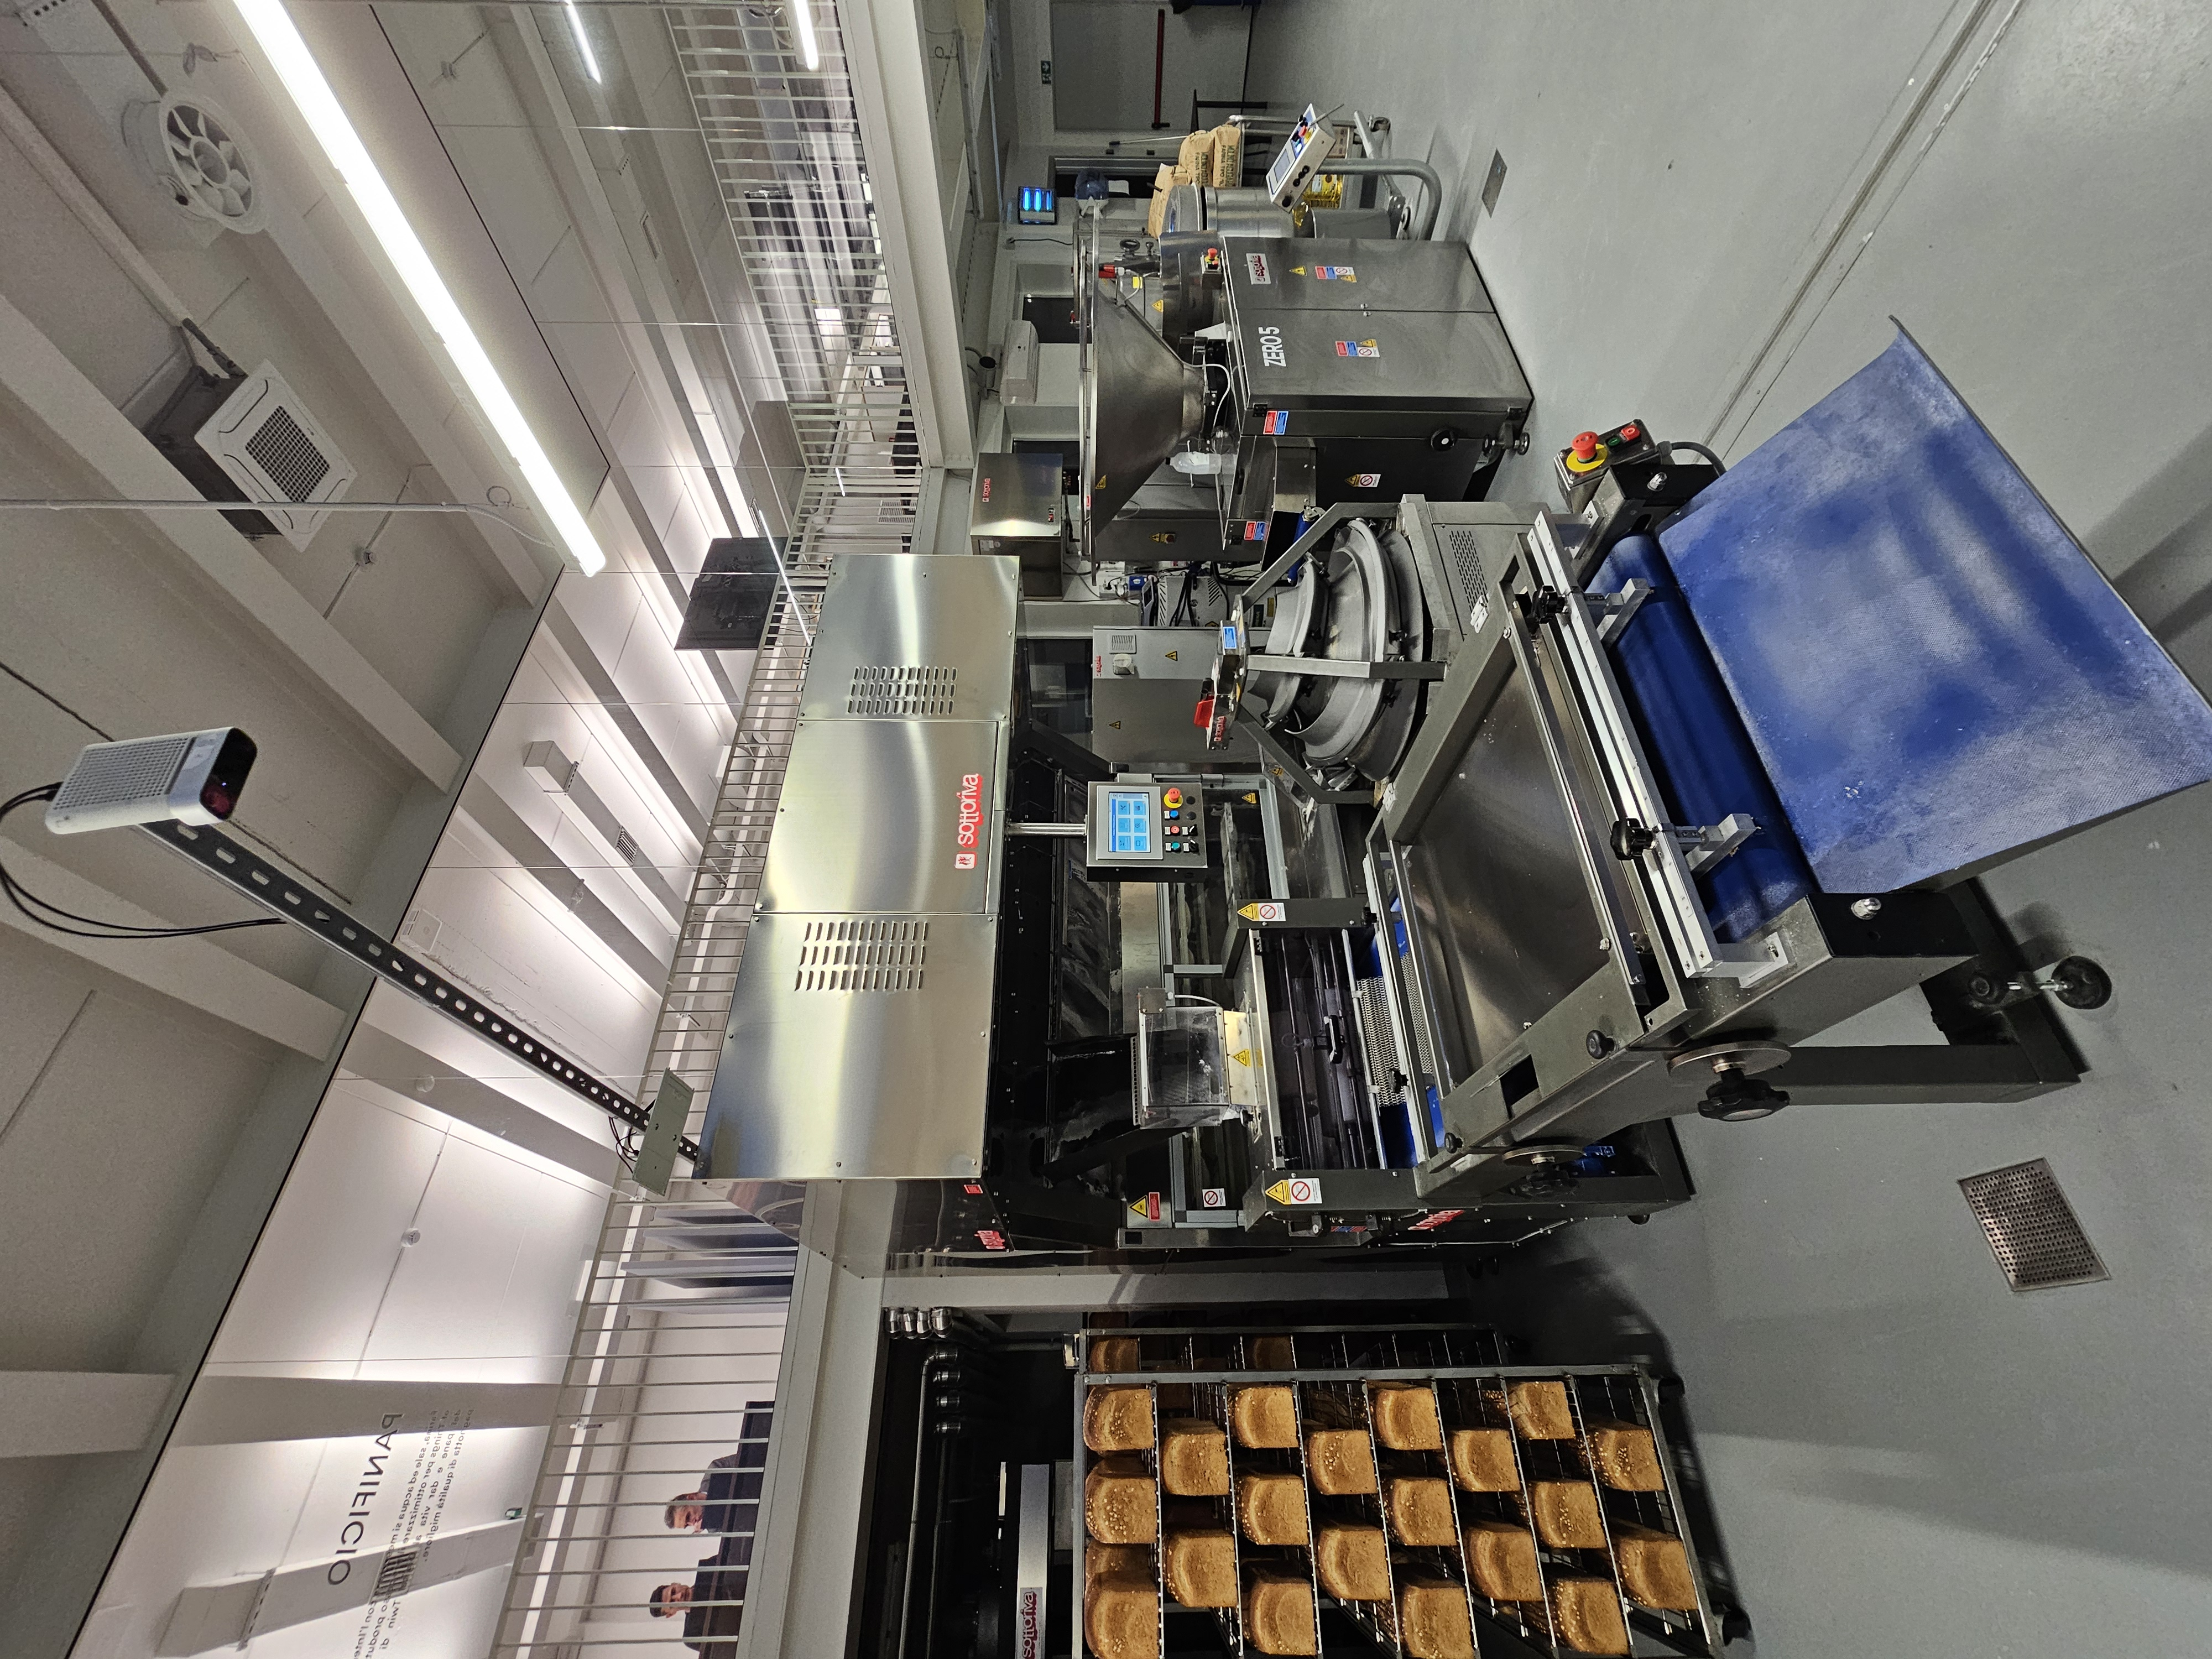
\includegraphics[scale=0.07, angle=-90]{images/Site1.jpg}
        \caption{Site 1: from here the dough balls come out and stop on the blue tray}
        \label{fig:site1}
    \end{subfigure}\hfill
    \begin{subfigure}[t]{0.48\textwidth}
        \centering
        \vspace{0pt}% allinea in alto
        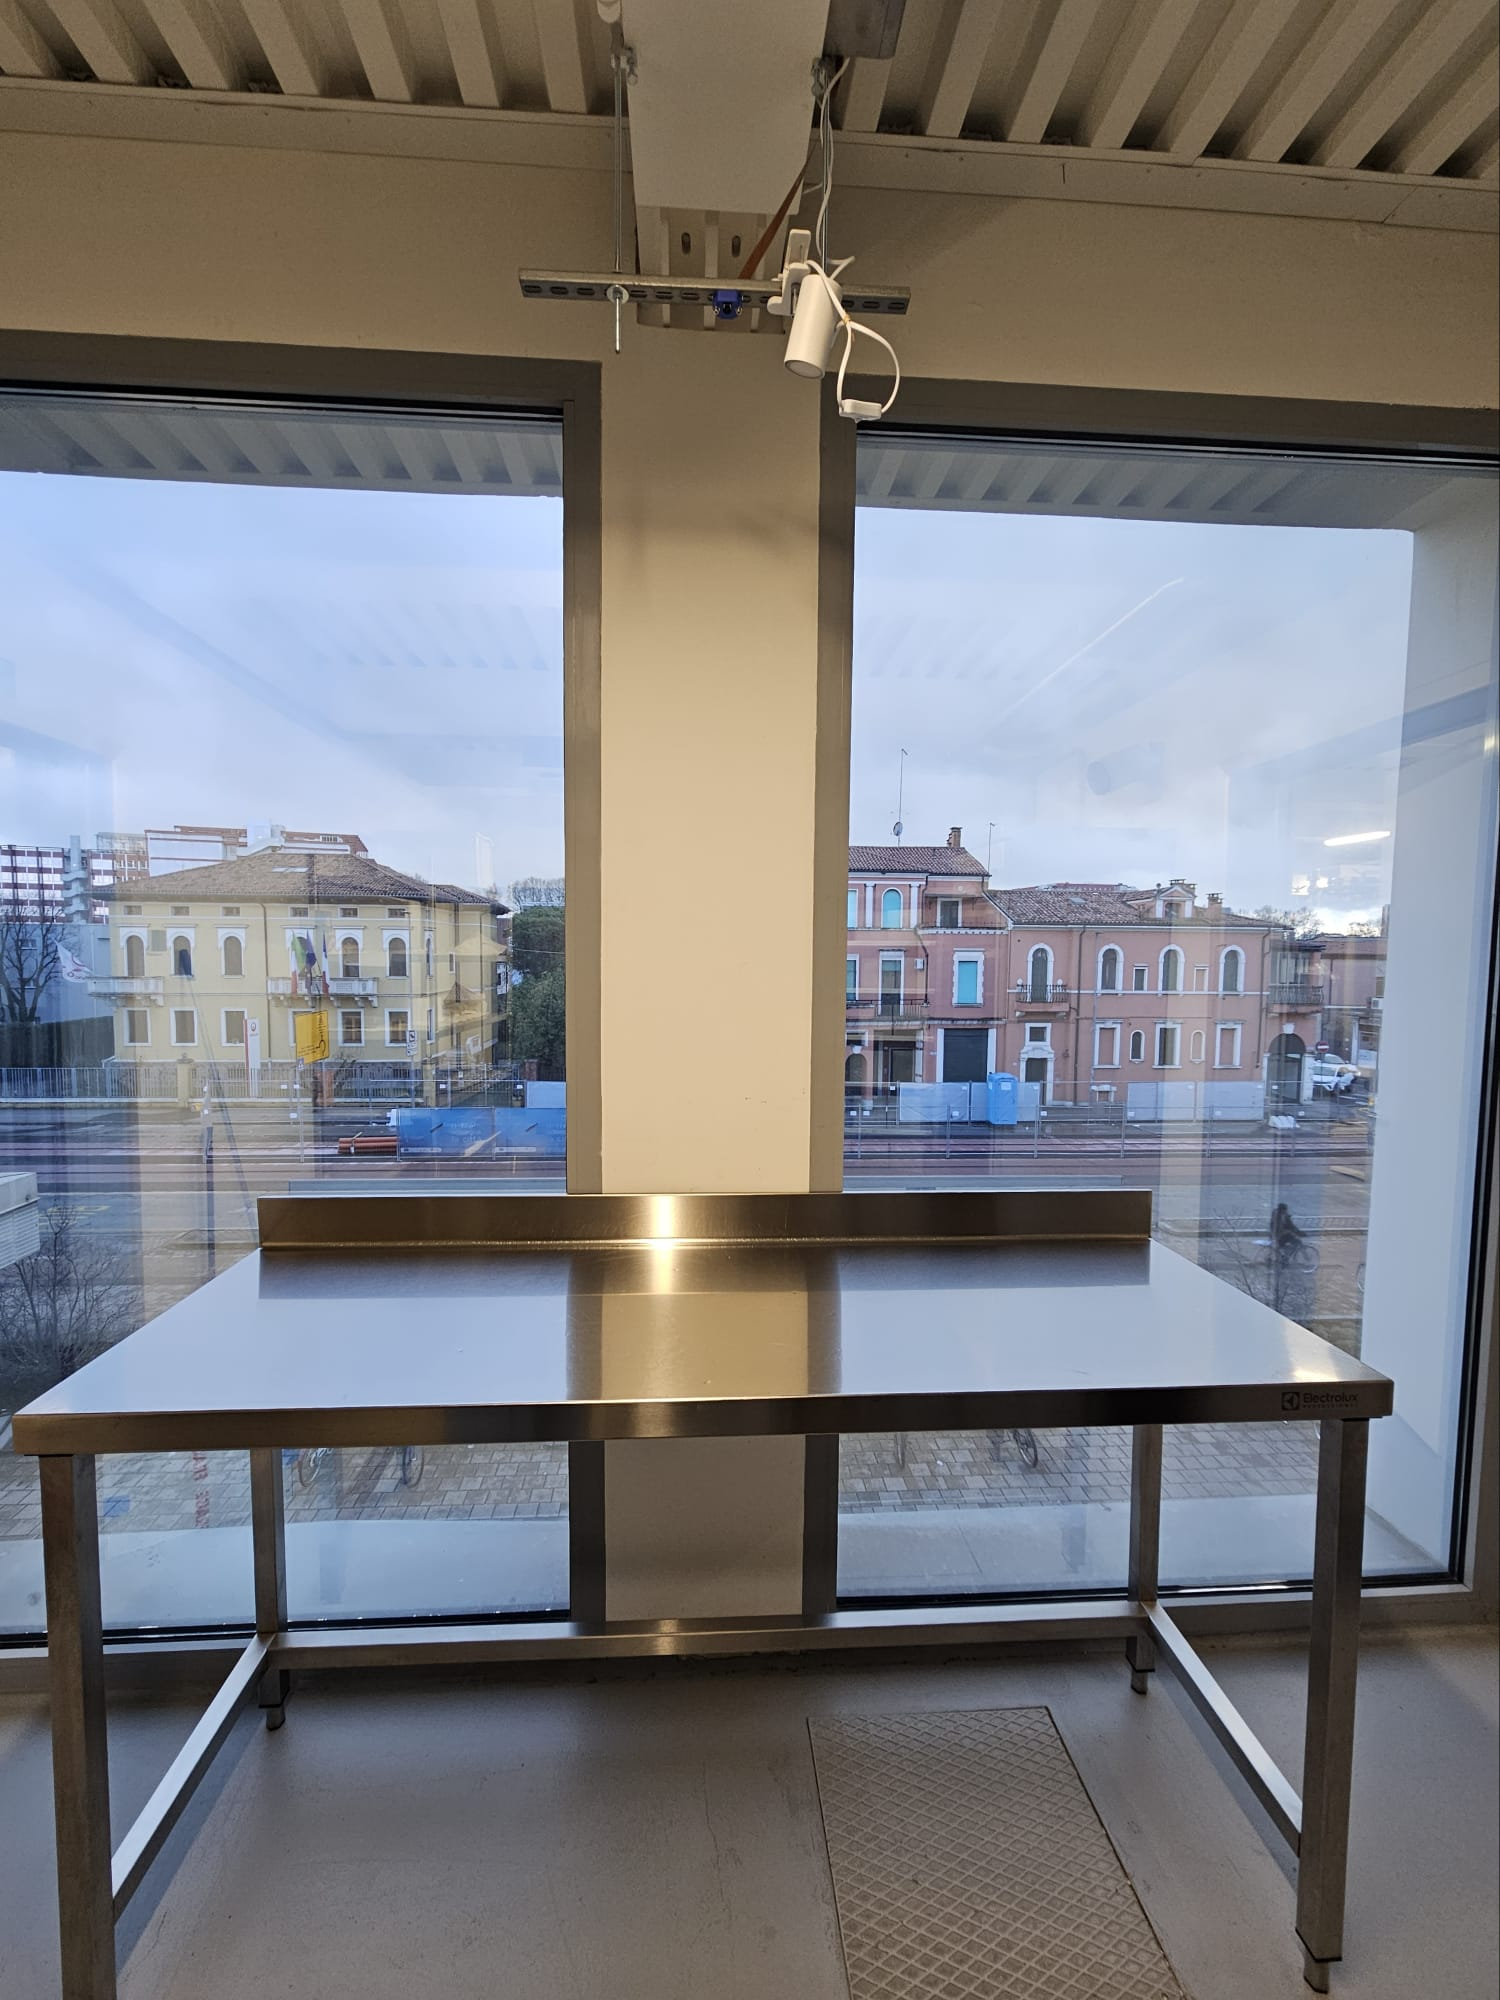
\includegraphics[scale=0.14]{images/sito2_giorno.jpeg}
        \caption{Site 2: area where bread is baked}
        \label{fig:site2}
    \end{subfigure}
    \caption{Overview of Site 1 and Site 2}
    \label{fig:sites12}
\end{figure}

Ultimately, once all the data have been extracted and processed, statistical distributions of dough ball volumes and anomaly scores for baked loaves are constructed. These distributions constitute the final analytical output of the system and provide a quantitative overview of production performance.

For each monitored variable, descriptive statistical indicators such as mean value, variance, and standard deviation are computed. The mean provides an estimate of the nominal production target, while the variance and standard deviation quantify dispersion and process variability. 

By analyzing both the distribution curves and their associated statistical descriptors, it becomes possible to evaluate the consistency and repeatability of the production process across different time intervals. In particular, deviations in volume distributions may indicate instability in the forming stage, whereas systematic shifts in anomaly-score distributions may reveal variations in baking conditions or product quality.
\newline

The resulting statistical summary therefore represents a quantitative decision-support tool for quality assessment. Rather than relying solely on qualitative visual inspection, the proposed framework enables objective measurement of process stability, variability, and deviation from expected operating conditions.

In this context, the thesis demonstrates how computer vision and embedded AI systems can be integrated into an industrial environment to transform raw sensory data into actionable statistical insights, bridging the gap between low-level image acquisition and high-level production performance evaluation. 



\section{Internship}
The thesis project was carried out during an internship period at \textbf{Flexsight Srl}.\\
During this period, responsibility for the \textbf{SMACT-related project} was assigned to the undersigned, and the project was developed primarily in an autonomous manner, with periodic collaboration and technical support from colleagues when required.\\\\
A key aspect of the work involved \textbf{on-site interactions at the production facility} to gather requirements and clarify technical specifications. This included structured discussions with project supervisors to better understand objectives, resolve ambiguities, and address feasibility constraints. Moreover, coordination with factory operators was essential to determine which activities could be performed without interfering with production, to identify operational limitations, and to adapt specific production procedures in order to enable proper data acquisition.\\
Extensive \textbf{information exchange} between supervisors, operators, and the project team significantly contributed to the design of the processing pipeline and to the final outcome of the project. The planning phase, combined with careful coordination of operator activities, ensured that data could be collected accurately, safely, and efficiently.\\

\subsection{Pipeline summary}
Following the planning phase, the \textbf{installation of the cameras and computing units} was carried out, together with the configuration of the acquisition parameters required to initiate the first operational stage: the Motion Detection phase. 
\\The project is, in fact, structured into three main components:
\begin{itemize}
  \item \textbf{Motion detection algorithm}:\\
  This module was designed to acquire and collect data by continuously monitoring the workstation areas (Figure \ref{fig:sites12}).
  This phase consisted of an automated and fully autonomous data collection process conducted over a period of two weeks. During this interval, the system operated without human intervention, continuously analyzing the scene and capturing relevant frames based on motion-triggered events.
  \\Cameras were oriented toward the production lines and configured to acquire images only when a product passed beneath them, triggering image acquisition. By defining appropriate motion thresholds and a Region of Interest (ROI), the dataset was built efficiently while minimizing redundant frames. 
  
  \item \textbf{Object detection}:\\
  For this component, a \textbf{DEIMv2} \cite{huang_real-time_2026} neural network was trained to detect bread loaves and dough balls using the dataset acquired in the previous phase. To train the network, the dataset was automatically labeled using \textbf{Language Segment-Anything} \cite{medeiros_luca-medeiroslang-segment-anything_2026}, a pretrained zero-shot model based on SAM2 (Segment Anything Model 2) and the GroundingDINO detection model. This model generates object masks and bounding boxes given a textual prompt, enabling automatic annotation of the training images.
  After training, the DEIMv2 network was able to produce bounding boxes identifying the spatial location of the products within the images.
  
  \item \textbf{Feature extraction}:\\
  Given the detected bounding boxes, volume-related features for dough balls and color-related features for baked loaves were extracted and aggregated to compute statistical distribution curves at the end of the process. Dough volume was estimated by reconstructing the point cloud within each bounding box using RGB-D information acquired by the Kinect sensor \cite{microsoft_azure_nodate}. Color-related features were computed by extracting statistical descriptors from the detected loaf regions in the RGB domain, enabling quantitative evaluation of crust browning and visual quality consistency.
\end{itemize}
\subsection{Practical challenges and system robustness}
% !TeX root = ../../tesi.tex

During the internship period and the initial deployment of the project, several practical challenges emerged that required dedicated engineering solutions.

\subsubsection{Robustness to Power Interruptions}

Throughout the design phase, it was observed that power interruptions occurred frequently within the production facility. Such events resulted in unexpected shutdowns of the embedded devices, interrupting the acquisition pipeline and compromising data continuity. Since the data acquisition process was required to operate autonomously for a two-week period without human intervention, this issue represented a critical risk to the success of the experimental campaign.

To mitigate this problem, the entire software architecture was designed to be resilient to power outages. In particular, the acquisition pipeline was encapsulated within a system service configured to automatically restart upon system boot.\cite{systemd_service_2026}

A \emph{system service} is a background process managed by the operating system's service manager (e.g., \texttt{systemd} in Linux-based systems). Services are designed to:

\begin{itemize}
    \item Automatically start at system boot,
    \item Restart upon unexpected failure,
    \item Run independently of user login sessions,
    \item Provide logging and monitoring capabilities.
\end{itemize}

At both sites, a user-level \texttt{systemd} service was implemented to execute the image acquisition script at startup. The service invokes a dedicated bash launcher script responsible for:

\begin{itemize}
    \item Navigating to the project directory,
    \item Activating the Python virtual environment,
    \item Launching the acquisition or processing script.
\end{itemize}

The service was configured with automatic restart policies (e.g., \texttt{Restart=always}) and a short restart delay to ensure that, upon restoration of electrical power, the system autonomously resumed operation without manual intervention.

This design choice significantly increased the reliability of the deployment and reduced maintenance overhead in the industrial environment.
%% TODO: qui potrei mettere un link al codice per il service

\subsubsection{Illumination Variability at Site 2}

An additional challenge was related to the physical configuration of Site 2. The bread extraction station is located on a metallic and reflective table positioned in front of two large windows (as shown in Figure~\ref{fig:site2}).

This configuration introduced significant illumination variability throughout the day due to:

\begin{itemize}
    \item Natural light intensity fluctuations,
    \item Direct sunlight reflections on the metallic surface,
    \item Shadows generated by operators during manual extraction.
\end{itemize}

Since the primary objective at Site 2 is visual quality assessment of baked bread through an anomaly detection model, uncontrolled illumination variations could directly affect the reliability of model predictions. In particular, variations in brightness and color temperature may introduce systematic biases in RGB-based inference.\cite{hoang_image-based_2025,kuhlechner_object_2025}

To ensure consistency and minimize illumination-related variability, a high-intensity artificial lighting source was installed above the acquisition area (as shown in Figure \ref{fig:faretto_sito2}).
\newline
The artificial illumination:

\begin{itemize}
    \item Increases dominance over ambient light,
    \item Reduces the impact of daylight fluctuations,
    \item Improves the repeatability and stability of color measurements.
\end{itemize}

By stabilizing the lighting conditions, the system achieves more reliable visual inference, which is critical for robust anomaly detection and for detecting deviations in the baking process.\cite{hoang_image-based_2025,kuhlechner_object_2025}

\begin{figure}[h]
    \centering
    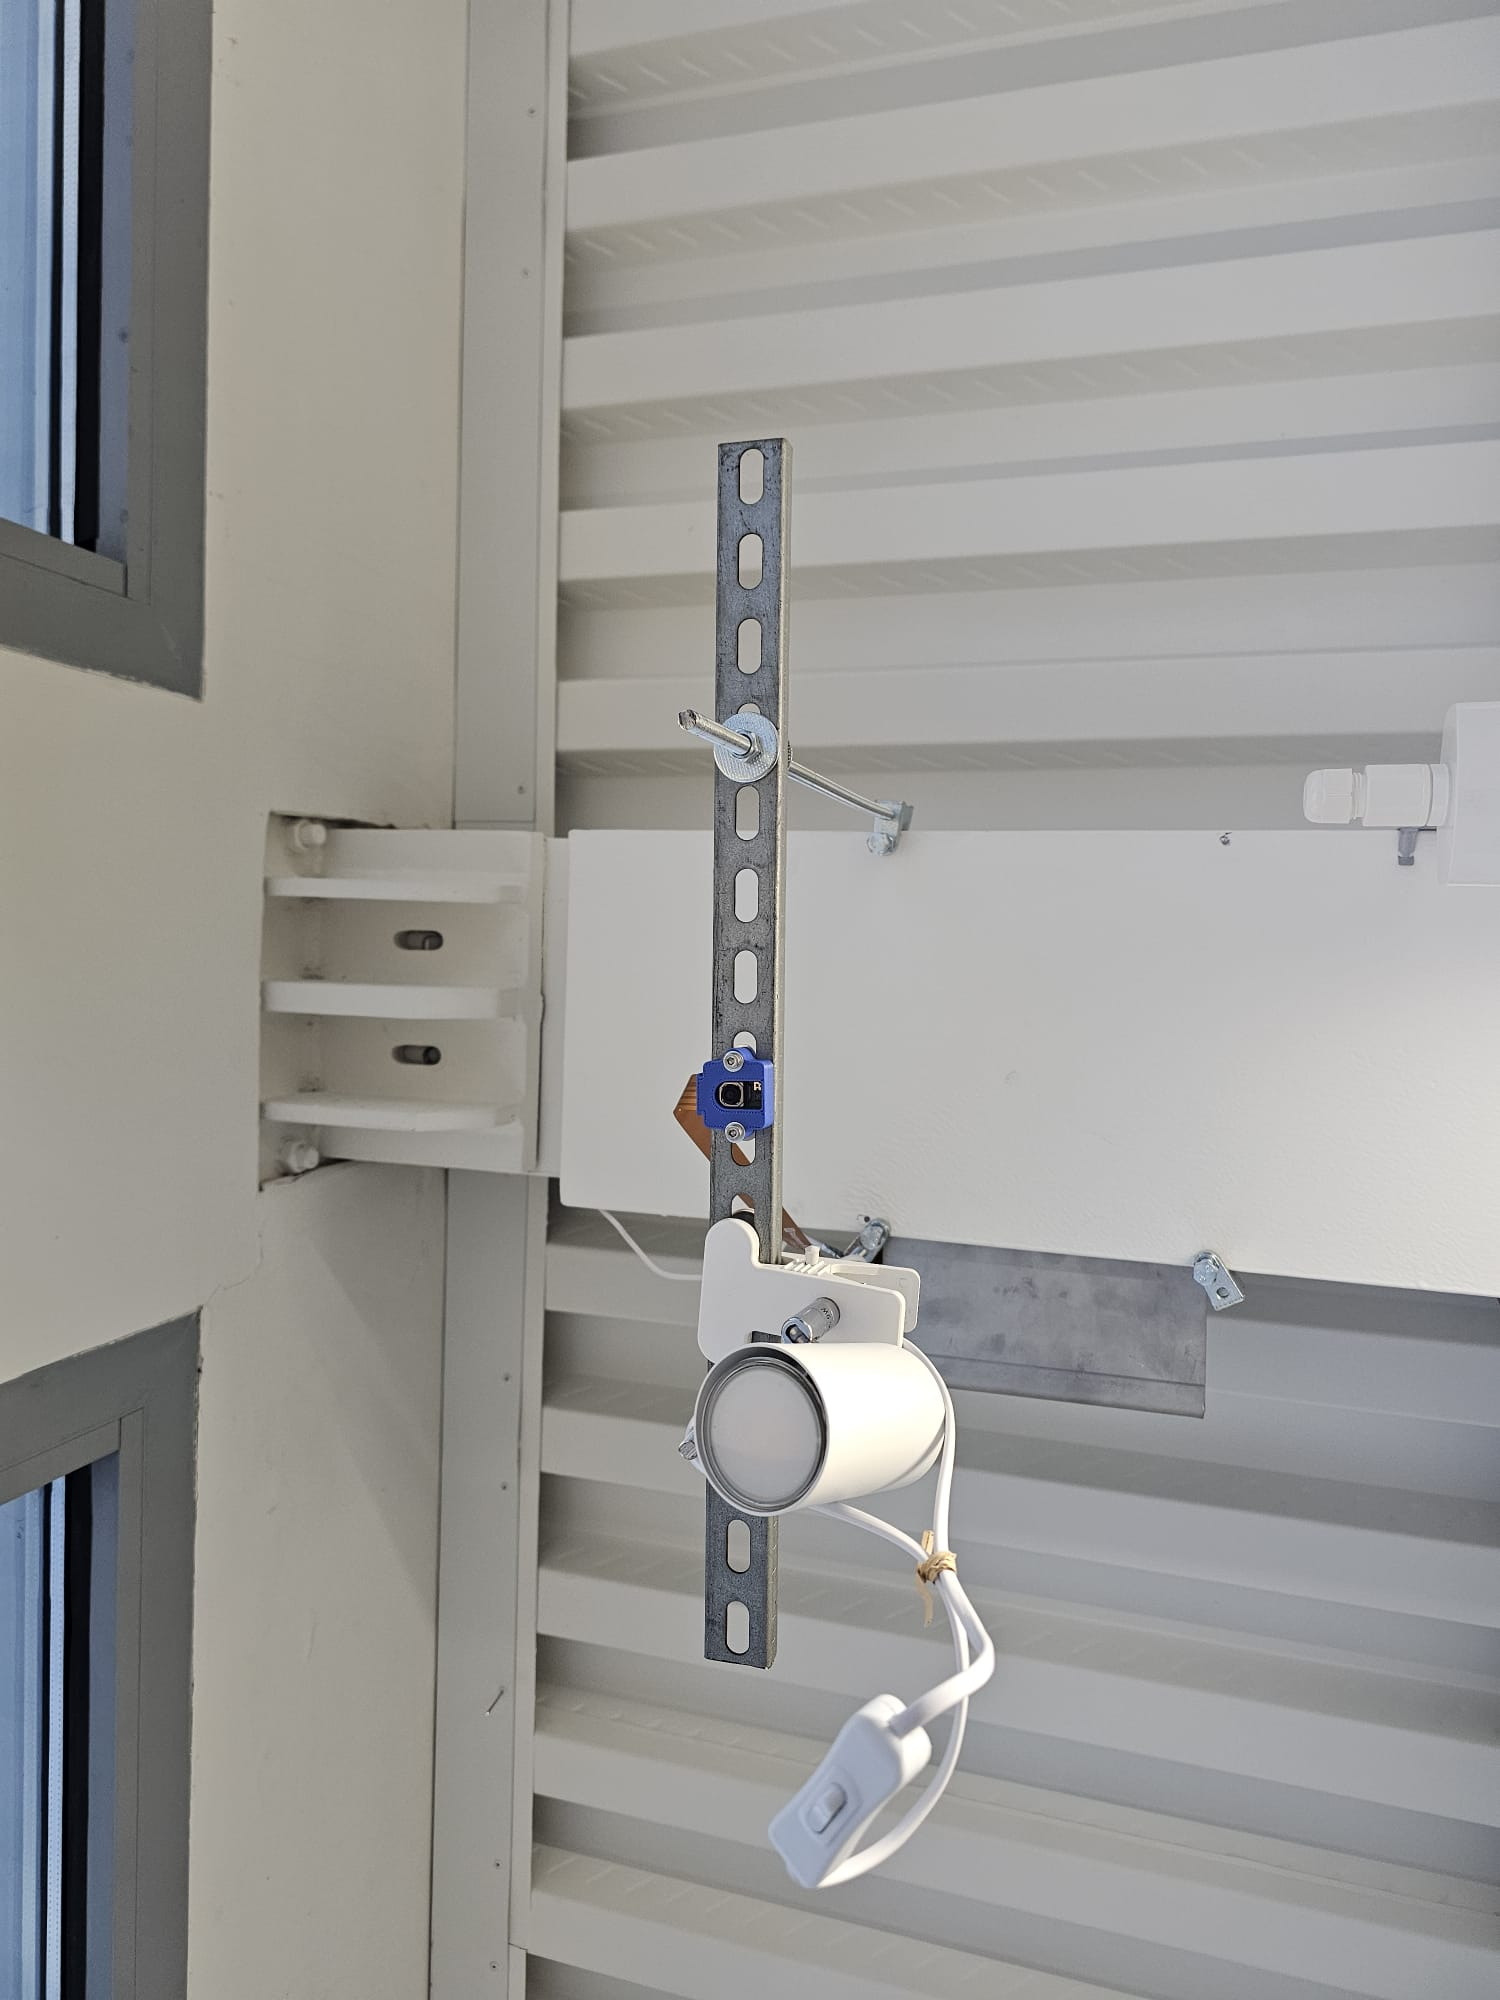
\includegraphics[width=0.5\linewidth, angle=90]{images/faretto_sito_2(1).jpeg}
    \caption{Light source placed next to the Raspberry Pi Camera to illuminate the scene and keep lighting as constant as possible}
    \label{fig:faretto_sito2}
\end{figure}

\subsection{Companies}
The internship was conducted in an industrial and research-oriented environment, enabling the practical application of computer engineering methodologies to real-world production scenarios.\\
The activities included the analysis of technical requirements, the design and implementation of software solutions, and the integration of hardware and software components within embedded and computer vision systems.

Moreover, the internship context facilitated continuous interaction with engineers and researchers, contributing to the development of professional competencies such as structured problem-solving, project organization, system reliability design, and compliance with industrial standards and operational constraints.

\subsubsection{Flexsight}

\subsubsection{SMACT}
 %File in cui è scritto il capitolo
\label{chapter:chapter_2} %Label per creare riferimenti al capitolo
% !TeX root = ../../tesi.tex

%Background Material
\chapter{Background Material}

\section{Computer Vision}
% !TeX root = ../../tesi.tex

Computer vision is a subfield of artificial intelligence (AI) that equips machines with the ability to process, analyze and interpret visual inputs such as images and videos. It uses machine learning to help computers and other systems derive meaningful information from visual data.\cite{ibm_what_nodate}

Object detection and image segmentation are two fundamental tasks in the field of computer vision, widely used for scene understanding and automated visual analysis. While both aim at identifying relevant objects within an image, they differ significantly in terms of output representation, computational complexity, and application scope.

\subsection{Object detection}
Object detection \cite{ibm_what_nodate} aims to pinpoint where objects are in digital images. It melds two learning techniques:
\begin{itemize}
    \item \textbf{Object localization} identifies the location of specific objects in an image by drawing bounding boxes around them.
    \item \textbf{Image classification} distinguishes the category to which objects belong.
\end{itemize} 
\begin{figure}[h]
    \centering
    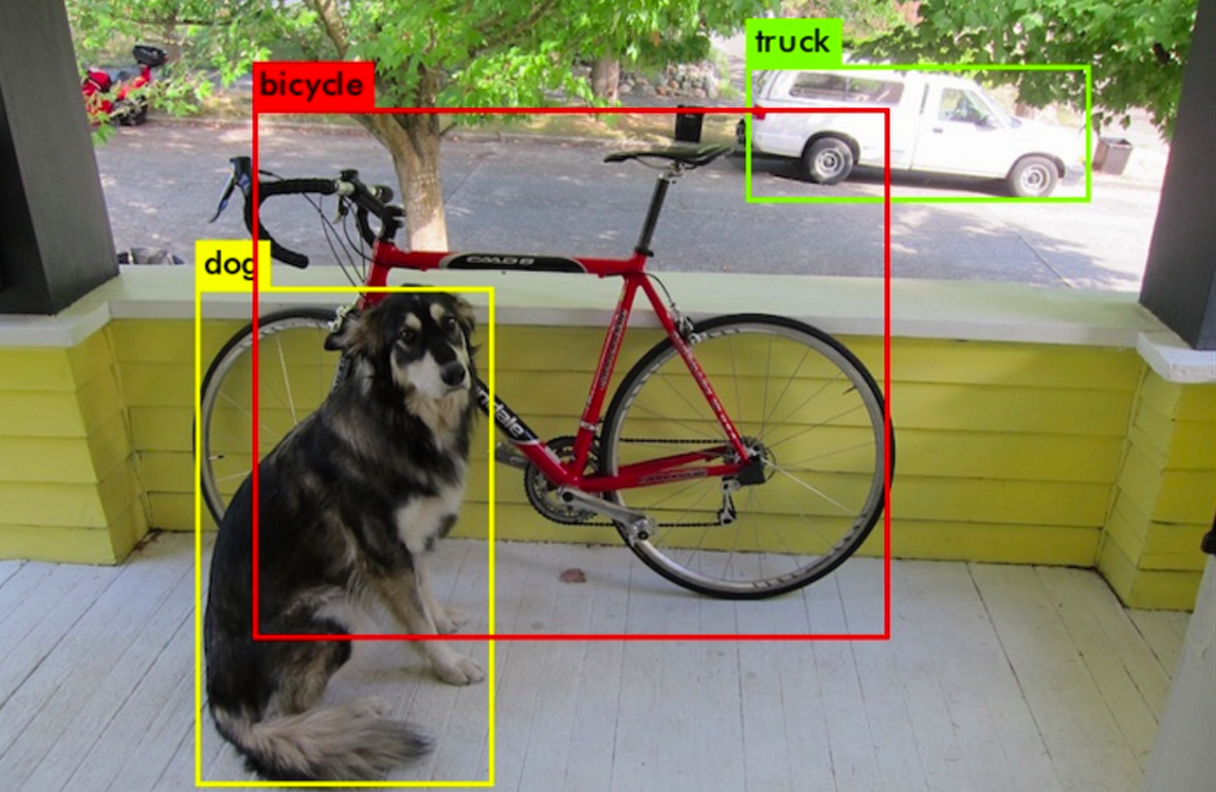
\includegraphics[scale=0.25]{images/object-detection.png}
    \caption{In the image, the detected objects are enclosed by bounding boxes \\and annotated with their corresponding class labels}
    \label{fig:object-detection}
\end{figure}

To evaluate object detection performance, the \textbf{Intersection over Union (IoU)} metric~\cite{ibm_what_2024} is commonly employed. IoU quantifies the overlap between a predicted bounding box and the corresponding ground-truth bounding box. It is defined as the ratio between the area of intersection and the area of union of the two bounding boxes:

\begin{equation}
\mathrm{IoU} = \frac{\mathrm{Area}(B_p \cap B_{gt})}{\mathrm{Area}(B_p \cup B_{gt})}
\end{equation}
where $B_p$ denotes the predicted bounding box and $B_{gt}$ the ground-truth bounding box.
IoU serves as a fundamental metric for assessing localization accuracy.

In addition to evaluation, IoU is also used during post-processing stages of object detection pipelines. Modern detection architectures often generate multiple bounding box proposals for a single object.
To eliminate redundant detections and retain only the most reliable prediction per object, a post-processing technique known as \textbf{Non-Maximum Suppression (NMS)} is applied.
NMS operates by first sorting all predicted bounding boxes according to their confidence scores in descending order. The bounding box with the highest confidence is selected as a valid detection, and all other boxes with an Intersection over Union (IoU) greater than a predefined threshold with respect to the selected box are suppressed. This process is repeated iteratively on the remaining boxes until no further candidates are available.
Formally, given a set of predicted bounding boxes $B_i$ with associated confidence scores $s_i$, NMS retains a subset of boxes such that highly overlapping detections are removed while preserving the most confident predictions. The IoU threshold plays a crucial role in determining the strictness of suppression: lower thresholds lead to more aggressive filtering, whereas higher thresholds allow more overlapping detections to remain.\\
NMS significantly improves the clarity and interpretability of detection results by ensuring that each object instance is represented by a single bounding box. 
\\

In conclusion, object detection provides a coarse yet computationally efficient form of localization, making it particularly suitable for \textbf{real-time applications} and scenarios in which precise object boundaries are not strictly required, as is the case in the present work.\\
This approach is generally designed to balance accuracy and computational efficiency, enabling their deployment in industrial environments characterized by constrained hardware resources.


\subsection{Image segmentation}
Image segmentation is a more precise, pixel-level version of object detection. It partitions a digital image into discrete groups of pixels known as image segments, then labels pixels according to their class or instance. \cite{ibm_what_nodate} \\
Depending on the task formulation, segmentation can be divided into:
\begin{itemize}
    \item \textbf{Semantic segmentation}: assigns each pixel in the image to a predefined category, without distinguishing between different object instances belonging to the same class.
    
    \item \textbf{Instance segmentation}: detects and segments each individual object instance in the image, producing a separate mask for each countable object (typically referred to as \emph{things}), while usually not distinguishing amorphous background regions such as sky or ground (\emph{stuff}).
    
    \item \textbf{Panoptic segmentation}: unifies semantic and instance segmentation by providing a complete scene understanding, where both individual object instances (\emph{things}) and uncountable background regions (\emph{stuff}) are segmented in a consistent and non-overlapping manner.\cite{ibm_what_2023}
\end{itemize} 
This fine-grained representation allows for an accurate description of object shapes and boundaries but comes at the cost of higher computational complexity and increased sensitivity to noise and illumination variations.
\begin{figure}[h]
    \centering
    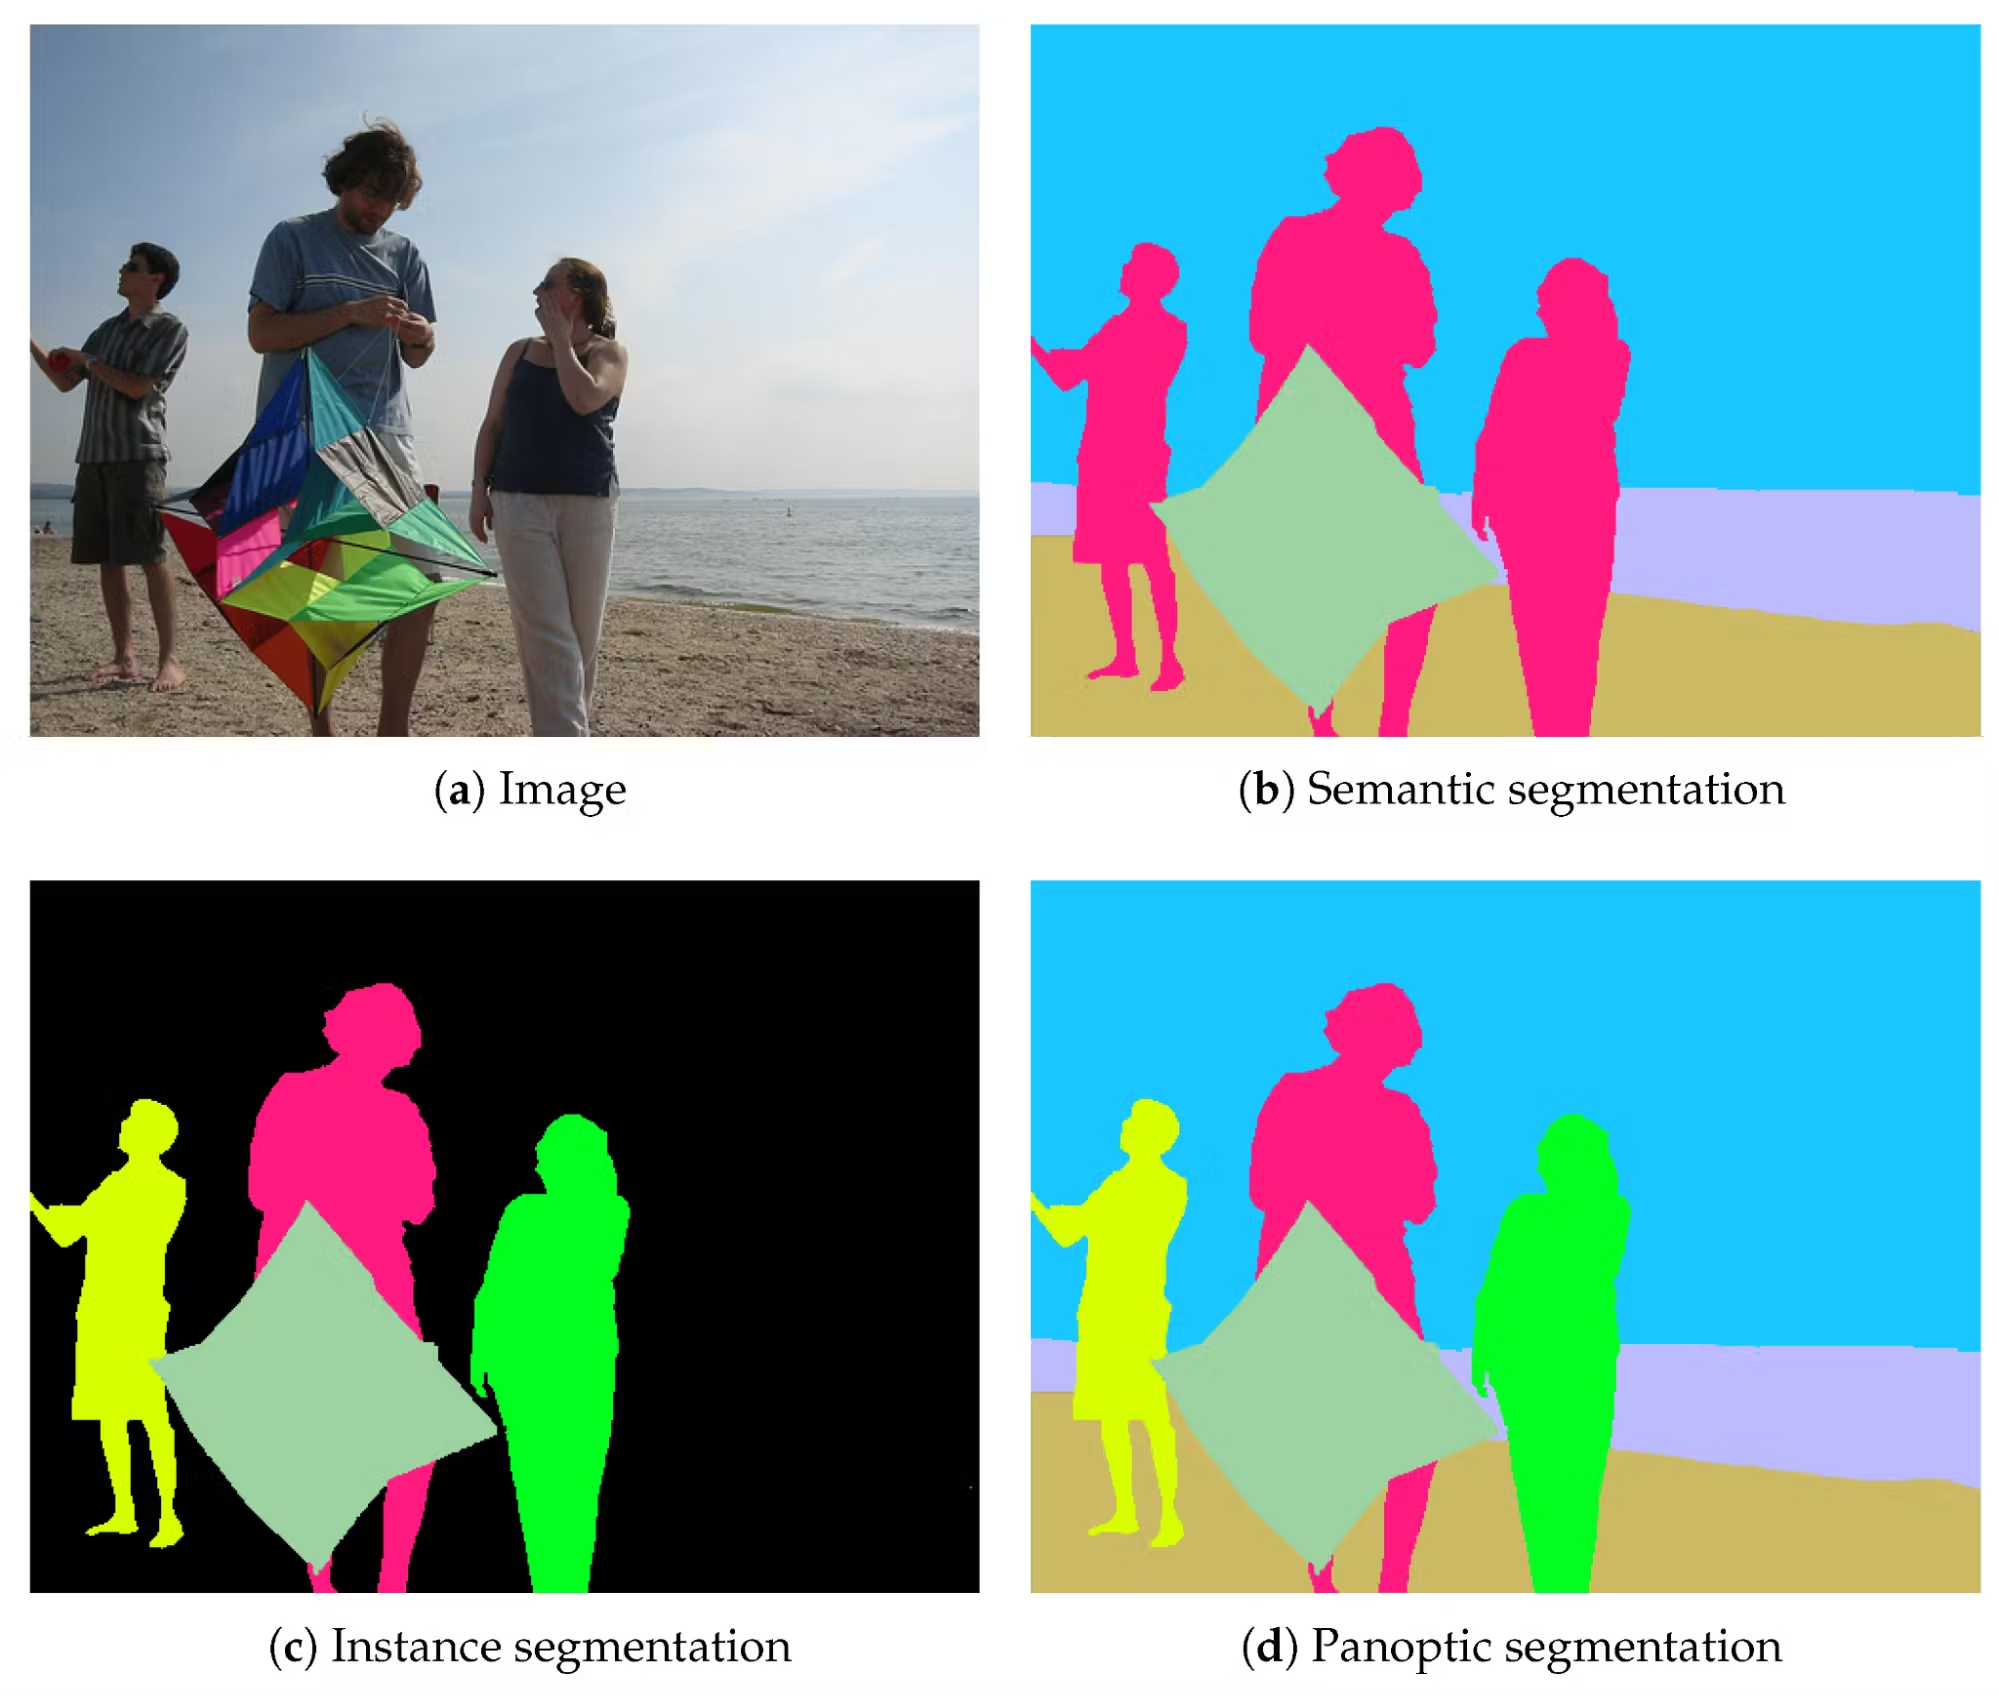
\includegraphics[scale=0.1]{images/segmentation.png}
    \caption{Different types of image segmentation}
    \label{fig:image-segmentation}
\end{figure}

Similarly to object detection, where the Intersection over Union (IoU) metric is widely adopted to evaluate the overlap between predicted and ground-truth bounding boxes, image segmentation relies on pixel-level overlap metrics.
\\
The most commonly used metric is the \textbf{Intersection over Union (IoU)}, also referred to as the \emph{Jaccard Index}. In the context of segmentation, IoU is computed as:

\begin{equation}
IoU = \frac{TP}{TP + FP + FN}
\end{equation}
where:
\begin{itemize}
    \item $TP$ (True Positives) represents the number of correctly predicted pixels belonging to a given class,
    \item $FP$ (False Positives) represents the number of pixels incorrectly assigned to that class,
    \item $FN$ (False Negatives) represents the number of pixels belonging to the class that were not correctly predicted.
\end{itemize}
Another commonly used metric is the \textbf{Dice Coefficient}, also known as the segmentation F1-score, defined as:

\begin{equation}
Dice = \frac{2TP}{2TP + FP + FN}
\end{equation}
The Dice coefficient is particularly popular in medical image segmentation, as it is more sensitive to small objects and class imbalance.

For instance segmentation and panoptic segmentation tasks, additional metrics such as \textbf{Average Precision (AP)} computed over mask IoU thresholds and \textbf{Panoptic Quality (PQ)} are often employed to jointly evaluate detection and segmentation performance.
These evaluation metrics provide a quantitative measure of the agreement between predicted segmentation masks and ground-truth annotations, enabling objective comparison between different models and approaches.
\subsection{Classical segmentation methods}
% !TeX root = ../../tesi.tex

\subsubsection{Clustering}
Clustering is a family of unsupervised methods aimed at grouping data samples according to \textbf{similarity} in a chosen feature space.\cite{mittal_comprehensive_2022} In image analysis, the samples typically correspond to pixels, superpixels, or local feature descriptors, while similarity may be defined in terms of color, intensity, texture, spatial position, or depth.\cite{mittal_comprehensive_2022}

Within computer vision, clustering can be exploited as a classical segmentation strategy.\cite{mittal_comprehensive_2022} The underlying idea is that pixels belonging to the same physical region often share common visual or geometric properties, and can therefore be grouped into homogeneous clusters. Once the clusters have been identified, they can be interpreted as candidate regions of interest or as a first approximation of the object masks.\cite{mittal_comprehensive_2022}

Among the simplest and most widely used approaches is \textbf{k-means clustering}, originally introduced by MacQueen,\cite{macqueen_some_1967} which partitions the input data into $k$ clusters by minimizing the within-cluster variance. When applied to images, k-means can be performed directly on RGB values, grayscale intensities, depth values, or combinations of these features.\cite{macqueen_some_1967,mittal_comprehensive_2022} This makes it particularly useful in scenarios where the target objects can be separated from the background through relatively simple low-level cues.\cite{mittal_comprehensive_2022}

In the present work, clustering is relevant because dough segmentation can benefit from the grouping of pixels or 3D points with similar visual or geometric properties. In the considered setup, color and depth cues can facilitate the separation between the dough and the surrounding scene. In this sense, clustering can be considered a useful classical tool for preprocessing, exploratory segmentation, or the extraction of candidate regions in controlled industrial environments.\cite{mittal_comprehensive_2022}
\begin{figure}[h]
    \centering
    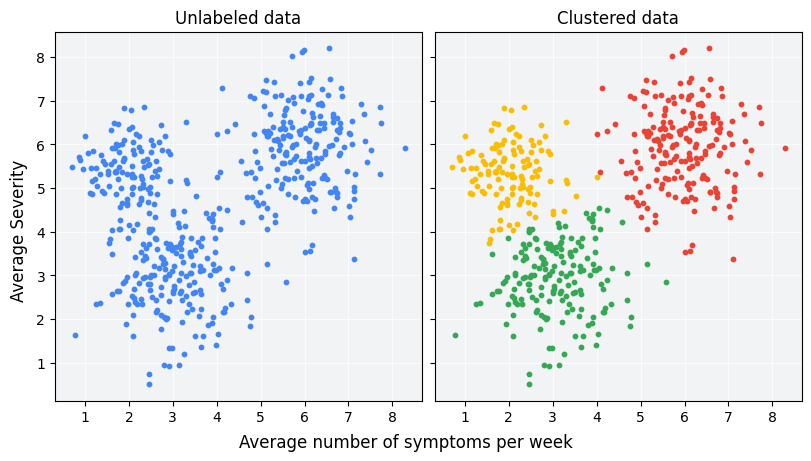
\includegraphics[scale=0.4]{images/clustering.png}
    \caption{Visualization of k-means clustering applied to an image, where pixels are grouped into clusters based on their similarity and distance in the feature-space. Each cluster is represented by a different color, illustrating how the algorithm partitions the image into distinct regions.}
    \label{fig:clustering}
\end{figure}


\subsubsection{Background subtraction}
Background subtraction is another classical strategy for foreground extraction. The main idea is to maintain a model of the background and compare the current observation against it, so as to identify the regions that differ significantly from the static part of the scene.\cite{opencv_background_subtraction_2026}

In vision-based applications, this approach is commonly used with static cameras to generate a foreground mask, that is, a binary image containing the pixels associated with the moving or changing objects in the scene.\cite{opencv_background_subtraction_2026} More generally, the same principle can be extended to cases in which the background is known or can be estimated in advance, and the goal is to isolate the objects of interest by removing the supporting surface or the stationary scene structure.
\begin{figure}[h]
    \centering
    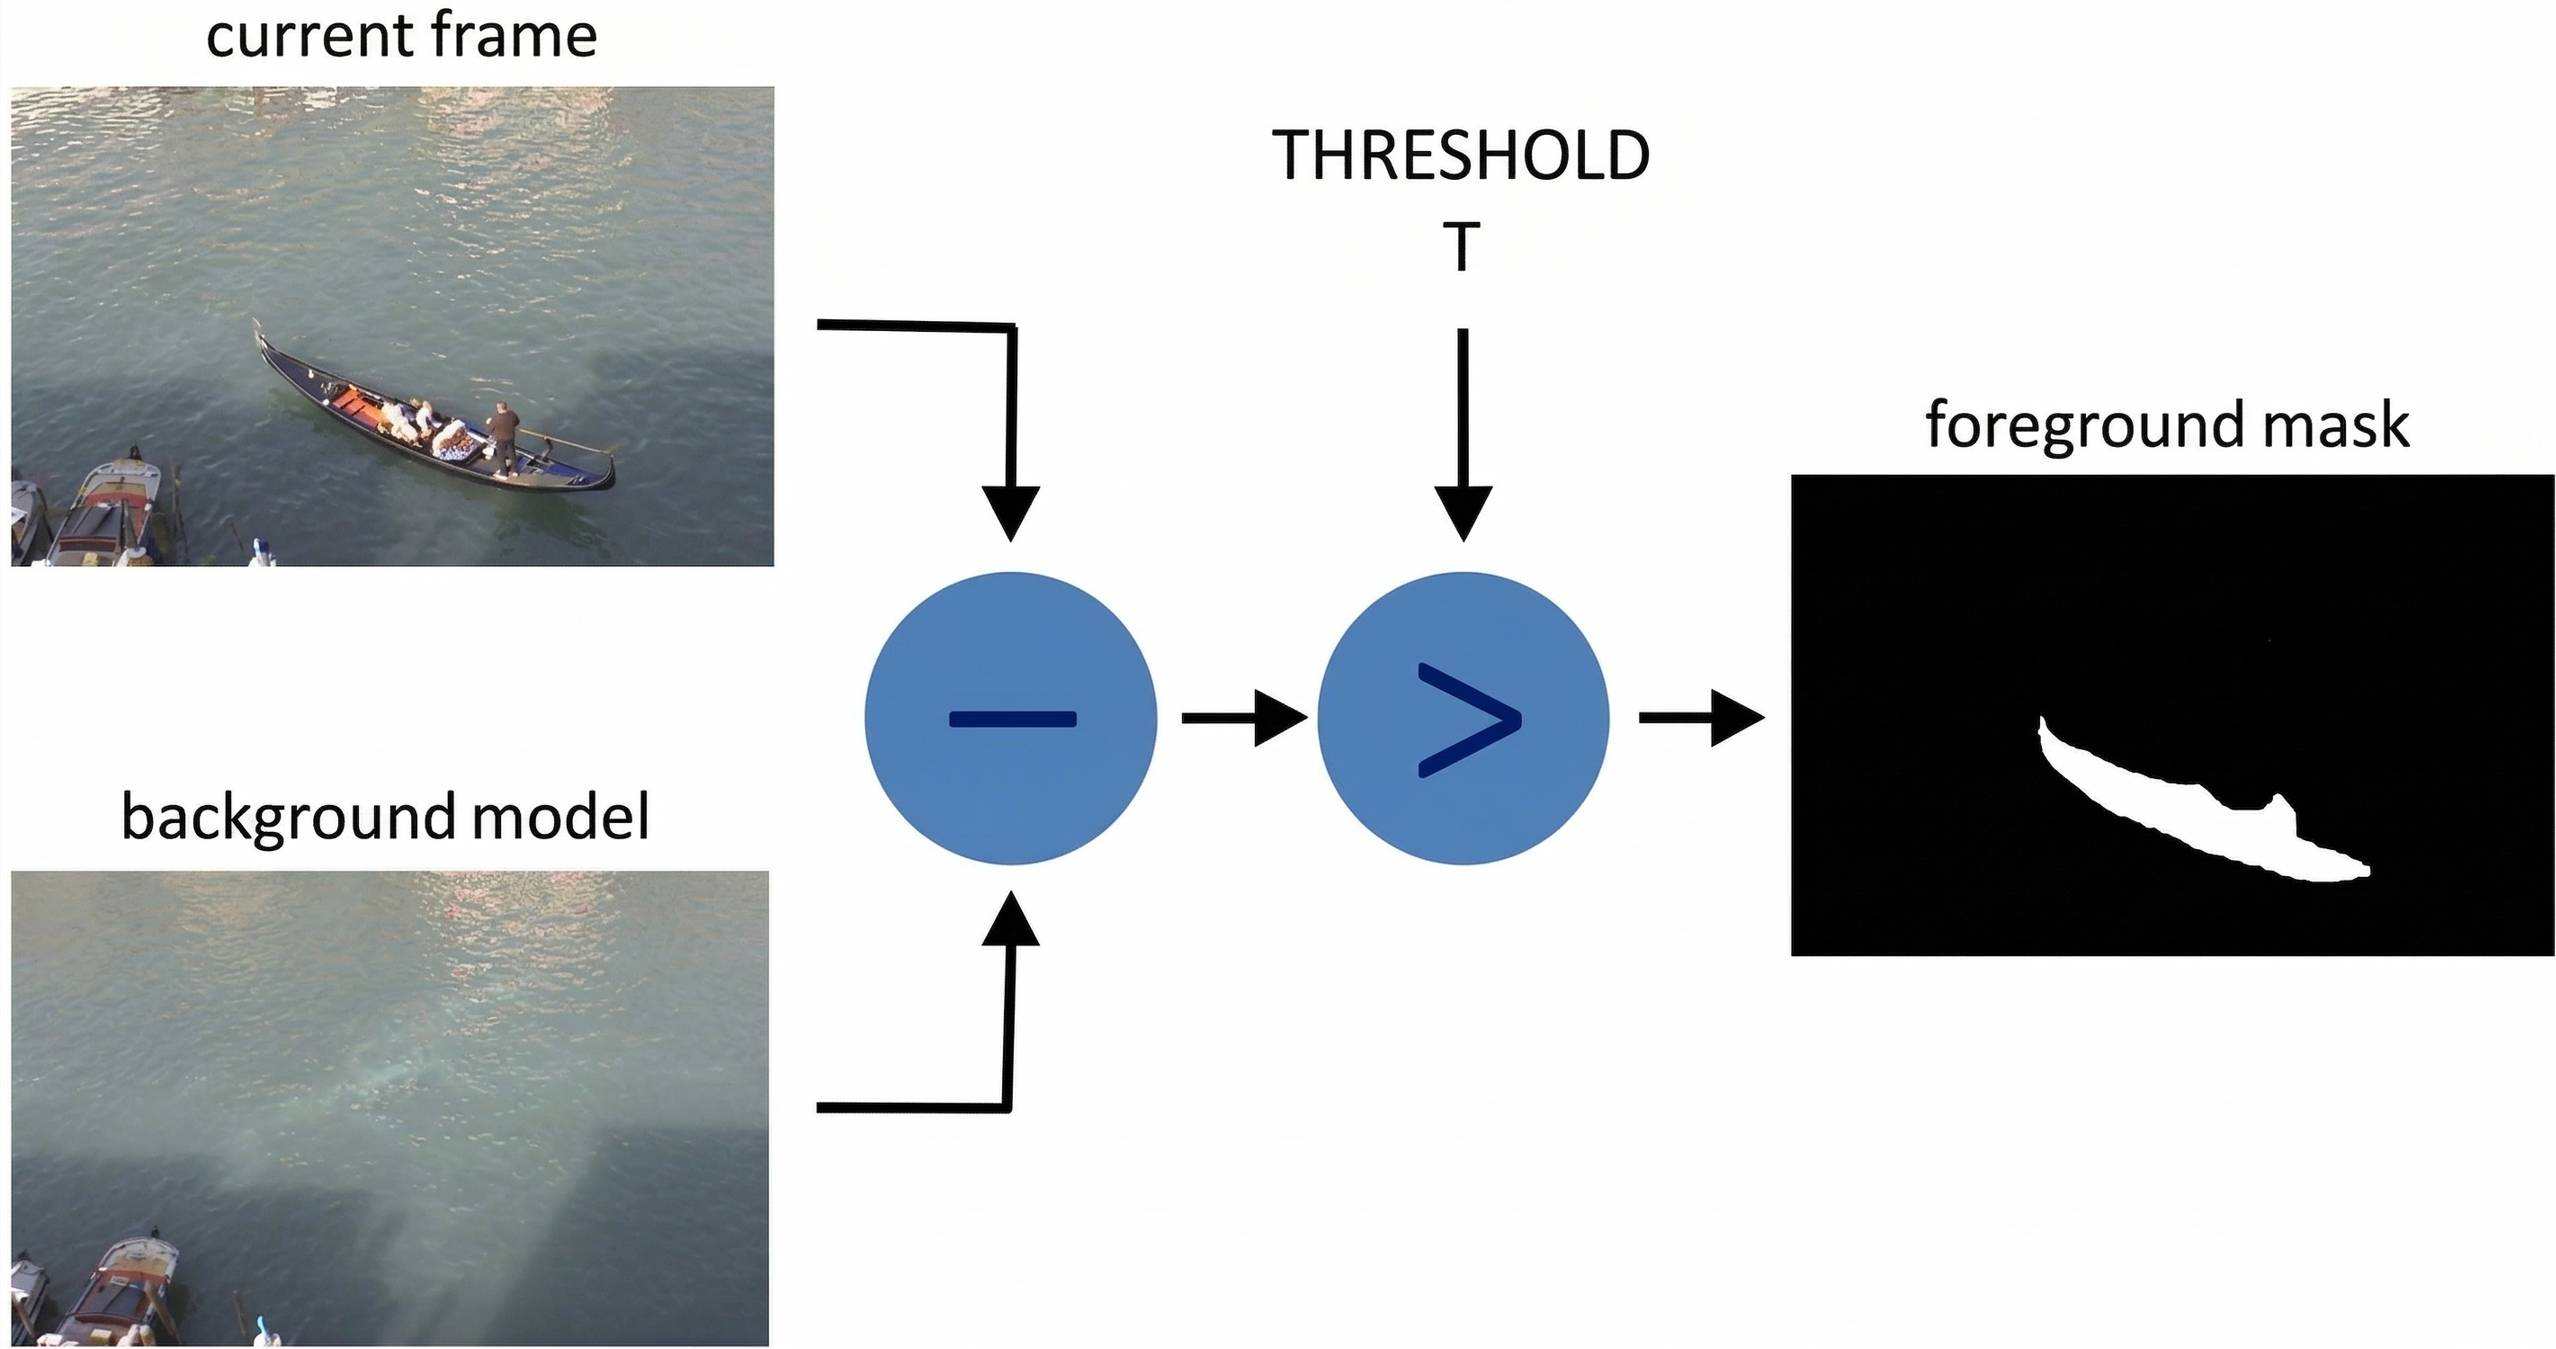
\includegraphics[width=0.6\textwidth]{images/Background_subtraction.png}
    \caption{Background subtraction example scheme.}
    \label{fig:background-subtraction}
\end{figure}

In the present work, this idea is relevant in two complementary ways. First, background subtraction is used in a non segmentation context in the RGB stream as part of the motion-detection module for dataset acquisition. Second, a conceptually similar foreground-background separation is exploited on depth information to isolate the dough from the supporting table before the subsequent geometric analysis.
Since the background (table) is static and can be reliably estimated in depth, this approach provides a computationally efficient way to segment the dough units without relying on complex learning-based models, which may be unnecessary in this controlled setting.

\subsection{Evaluation metrics}
In semantic segmentation, IoU is often computed independently for each class and then averaged across classes, yielding the \textbf{mean Intersection over Union (mIoU)}.\cite{tensorflow_mean_iou_2026,muller_guideline_2022} This metric is particularly informative in multi-class settings because it penalizes both over-segmentation and missed regions.

Other commonly adopted metrics include \textbf{precision} and \textbf{recall}, defined at pixel level as follows:\cite{sklearn_precision_recall_2026}

\begin{equation}
Precision = \frac{TP}{TP + FP}
\end{equation}

\begin{equation}
Recall = \frac{TP}{TP + FN}
\end{equation}

Precision measures how many of the pixels predicted as positive are actually correct, while recall measures how many of the truly positive pixels are successfully retrieved by the model.\cite{sklearn_precision_recall_2026} Their harmonic mean is given by the \textbf{F1-score}, or equivalently the \textbf{Dice coefficient}, which is widely used in segmentation tasks.\cite{muller_guideline_2022}

\begin{equation}
F1 = Dice = \frac{2TP}{2TP + FP + FN}
\end{equation}

In binary segmentation problems or anomaly-detection settings, the \textbf{Area Under the Receiver Operating Characteristic Curve (AUROC)} can also be used. AUROC evaluates the model's ability to discriminate between positive and negative pixels across different decision thresholds.\cite{sklearn_roc_auc_2026} However, in strongly imbalanced segmentation tasks, overlap-based metrics such as IoU or Dice are often considered more informative.\cite{muller_guideline_2022}

For instance segmentation, COCO-style evaluation commonly reports \textbf{Average Precision (AP)} over mask IoU thresholds, while panoptic segmentation is commonly evaluated with \textbf{Panoptic Quality (PQ)}.\cite{detectron2_coco_evaluation_2020,kirillov_panoptic_2019}
These evaluation metrics provide a quantitative measure of the agreement between predicted segmentation masks and ground-truth annotations, enabling objective comparison between different models and approaches.

\section{Neural networks}
% !TeX root = ../../tesi.tex

Neural networks (NNs) are parametric function approximators inspired by the distributed information-processing paradigm of biological nervous systems. At a conceptual level, an NN is composed of interconnected layers of artificial neurons, where each neuron receives a set of inputs, combines them linearly through trainable weights and biases, and then applies a non-linear activation function. By stacking multiple layers, the network implements a nested composition of transformations that can model highly non-linear input--output relationships \cite{goodfellow_deep_2016}. During training, the parameters are adjusted so as to minimize a task-specific loss function, thereby enabling the network to progressively improve its predictions from data \cite{goodfellow_deep_2016}.

\begin{figure}[h]
    \centering
    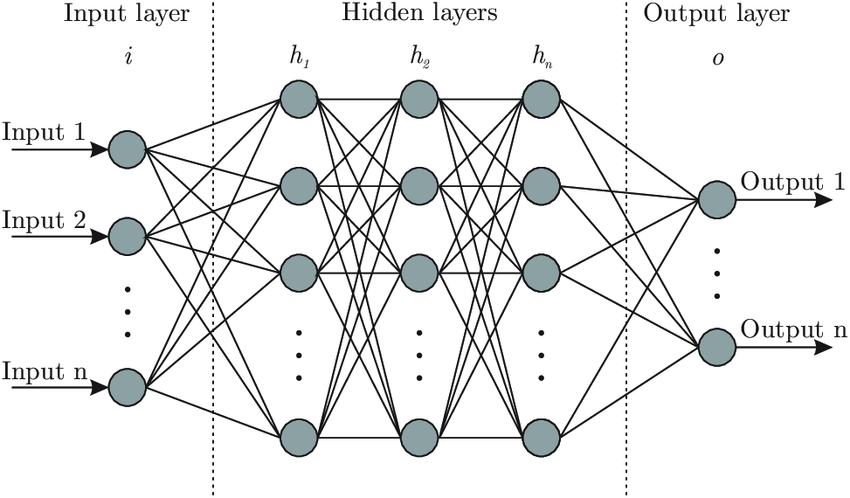
\includegraphics[width=0.5\textwidth]{images/NN.png}
    \caption{Schematic representation of a feedforward neural network with multiple hidden layers. Each layer applies a linear transformation followed by a non-linear activation, enabling progressively richer representations of the input.}
\end{figure}

The optimization of neural networks is typically performed through \textbf{gradient descent} and its stochastic variants. After computing the loss associated with a prediction, gradient descent updates the model parameters in the direction that most reduces the loss, with the size of each update controlled by the learning rate. Backpropagation provides the mechanism that makes this process computationally feasible: by applying the chain rule from the output layer back to the earlier layers, it efficiently computes the gradient of the loss with respect to each parameter in the network \cite{rumelhart_learning_1986,goodfellow_deep_2016}. Together, gradient-based optimization and backpropagation allow neural networks to learn complex functions directly from data.

\begin{figure}[h]
    \centering
    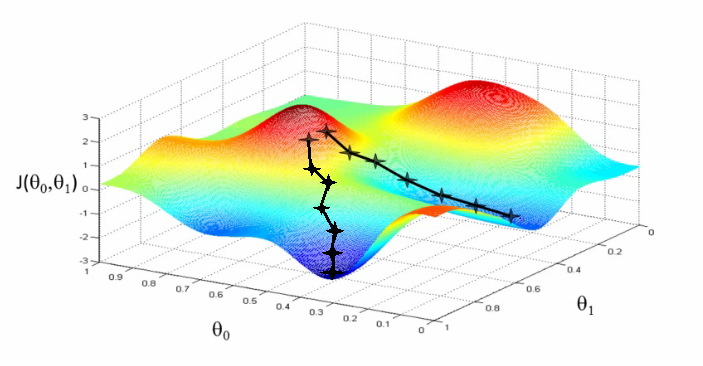
\includegraphics[width=0.5\textwidth]{images/Gradient_descent.png}
    \caption{Illustration of gradient descent over a loss surface. At each iteration, the parameters are updated in the direction of the negative gradient so as to reduce the loss.}
\end{figure}

\subsection{Deep Learning}
While the term neural network refers broadly to a family of trainable models composed of interconnected artificial neurons, \textbf{deep learning} denotes the specific setting in which these models contain multiple representation-learning layers arranged in depth \cite{goodfellow_deep_2016}. The practical importance of depth lies in its ability to learn hierarchical representations: lower layers tend to encode simpler patterns, whereas deeper layers combine them into progressively more abstract and task-relevant features \cite{lecun_deep_2015,goodfellow_deep_2016}. This property distinguishes deep learning from earlier machine learning pipelines, in which feature extraction was often designed manually before classification or regression.

By making end-to-end representation learning possible, deep learning allows the model to infer useful features directly from raw or weakly processed data rather than relying on handcrafted descriptors \cite{goodfellow_deep_2016}. This shift has been one of the main reasons for the remarkable progress observed across computer vision, speech, and natural language processing. At the same time, the high representational capacity of deep models generally \textbf{requires large datasets}, substantial computational resources, and careful optimization procedures in order to achieve strong generalization performance \cite{lecun_deep_2015}. A decisive milestone in this development was the success of deep convolutional networks in large-scale visual recognition, which accelerated both scientific interest and industrial adoption \cite{krizhevsky_imagenet_2012}.
\begin{figure}[h]
    \centering
    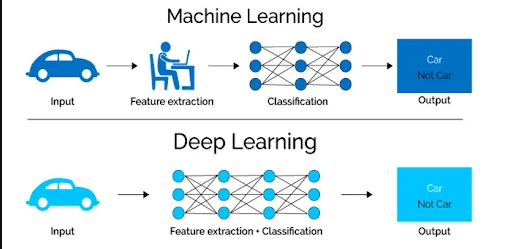
\includegraphics[width=0.5\textwidth]{images/DL.png}
    \caption{Schematic representation of a deep neural network, where feature representations are learned across multiple layers of abstraction and not manually engineered.}
\end{figure}

\subsection{Convolutional Neural Networks}
Among deep architectures for visual data, \textbf{Convolutional Neural Networks (CNNs)} have long represented the dominant paradigm. Their design is based on local receptive fields, \textbf{shared convolutional kernels}, and hierarchical feature extraction as for deep learning nets, which introduce useful inductive biases such as translation equivariance and improved parameter efficiency \cite{lecun_gradient-based_1998,goodfellow_deep_2016}. In a convolutional layer, the same learnable kernel is applied across different spatial positions of the input image, producing feature maps that respond to recurring \textbf{local patterns}. This combination of local connectivity and parameter sharing drastically reduces the number of trainable parameters, making CNNs more efficient to optimize and, in many practical settings, less data-hungry than generic dense architectures for visual tasks \cite{goodfellow_deep_2016,lecun_gradient-based_1998}. 

The use of kernels is particularly well suited to images because relevant visual structures, such as edges, corners, textures, and simple shapes, are inherently local. By learning detectors for these local patterns and reusing them across the whole image, CNNs can extract meaningful features while preserving spatial structure. This property generally improves generalization to unseen images and makes CNNs effective even when computational resources or dataset sizes are more limited than those required by less structured architectures \cite{goodfellow_deep_2016,lecun_gradient-based_1998}. In practice, early layers tend to capture low-level structures, whereas deeper layers encode increasingly abstract semantic patterns. Additional operations such as spatial downsampling or pooling further enlarge the effective receptive field and support the progressive aggregation of information across layers \cite{lecun_gradient-based_1998}. This hierarchical organization explains the effectiveness of CNNs in tasks such as image classification, object detection, and semantic segmentation.

\begin{figure}[h]
    \centering
    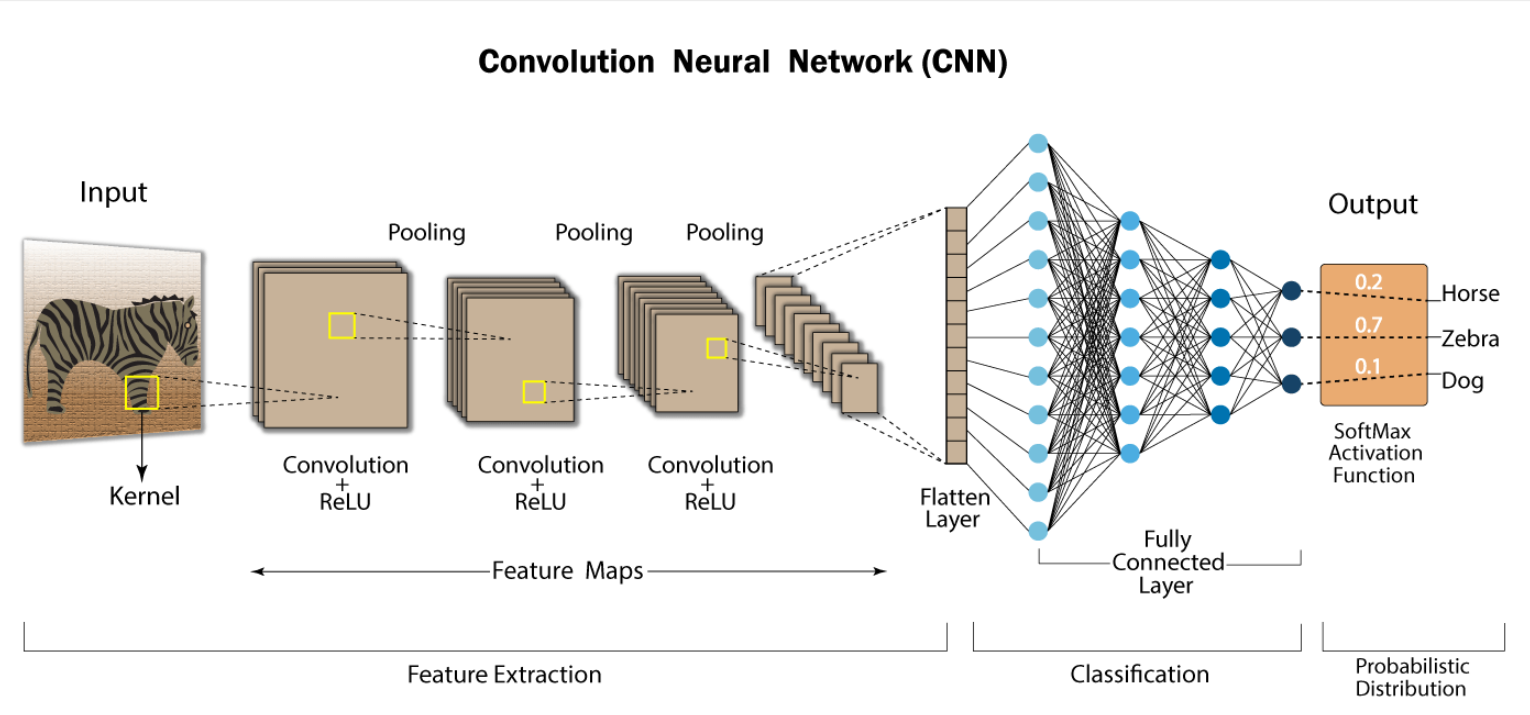
\includegraphics[width=0.52\textwidth]{images/CNN.png}
    \caption{Typical convolutional neural network architecture for visual processing, in which convolutional and downsampling stages progressively extract hierarchical features from the input image.}
\end{figure}

In the context of this thesis, neural networks, deep learning, and CNNs provide the conceptual foundation for the architectures discussed in the following sections. Vision Transformers and RT-DETR will therefore be introduced as successive developments built upon, or reacting to, this baseline \cite{dosovitskiy_image_2021,zhao_detrs_2024}.

\section{Vision Transformers (ViT)}
In recent years, \textbf{Vision Transformers (ViT)} \cite{dosovitskiy_image_2021} have progressively reshaped the landscape of computer vision, offering an alternative to the long-standing dominance of convolutional neural networks (CNNs). Originally inspired by Transformer architectures in natural language processing, ViTs process images as sequences of patches rather than as continuous grids.

More specifically, an input image is divided into fixed-size patches, which are then linearly projected into embedding vectors and treated as tokens. These tokens are processed through a Transformer encoder, where self-attention mechanisms allow the model to capture relationships between distant regions of the image. This ability to model global context is one of the main strengths of ViTs, especially when compared to CNNs, whose receptive field grows only progressively with depth.

This architectural choice brings several advantages. ViTs tend to learn richer semantic representations, making them particularly effective in recognizing complex visual patterns and capturing long-range dependencies. Additionally, their performance scales well with larger datasets and model sizes, often outperforming CNN-based approaches in high-capacity regimes.

However, these benefits come with non-negligible drawbacks. The self-attention operation has a quadratic complexity with respect to the number of tokens, which makes ViTs computationally demanding, especially for high-resolution inputs. This aspect has historically limited their use in real-time or resource-constrained environments.

Despite these limitations, ViTs have become a key component in many modern computer vision pipelines. In particular, they are widely used as backbone networks in object detection and segmentation frameworks, where their ability to extract both global context and fine-grained features proves especially valuable. As also highlighted in the analyzed material \cite{your_pdf_ref}, recent models such as DINO-based architectures demonstrate how ViT backbones can provide strong semantic representations while still being adapted for efficient downstream tasks.
\section{RT-DETR}
% !TeX root = ../../tesi.tex

RT-DETR (Real-Time Detection Transformer) extends the DETR paradigm toward real-time object detection by preserving its end-to-end formulation while explicitly addressing the latency and computational limitations that hindered earlier transformer-based detectors \cite{zhao_detrs_2024}. As in DETR, object detection is formulated as a set prediction problem, so that the model directly outputs a fixed set of detections without relying on heuristic post-processing such as Non-Maximum Suppression (NMS). The main contribution of RT-DETR lies in making this formulation practical for real-time scenarios.
\begin{figure}[h]
    \centering
    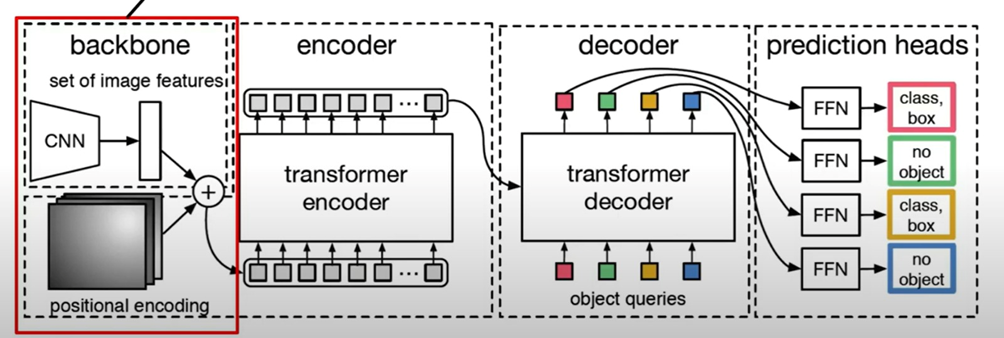
\includegraphics[scale=0.7]{images/DETR.png}
    \caption{Original DETR architecture.}
    \label{fig:DETR_architecture}
\end{figure}

From an architectural perspective, RT-DETR retains the standard backbone--encoder--decoder structure of DETR-style detectors, with prediction heads for object classification and bounding box regression. In this pipeline, the encoder is responsible for processing and fusing the visual features extracted by the backbone, so as to build a more informative representation of the scene before object queries are introduced. The decoder then takes these encoded features together with a set of object queries and iteratively refines them into final detections, progressively improving class predictions and bounding box localization. However, RT-DETR introduces several refinements designed to improve the accuracy--speed trade-off. In particular, the model employs an \textbf{efficient hybrid encoder} to process multi-scale visual features more efficiently by decoupling intra-scale interaction from cross-scale fusion \cite{zhao_detrs_2024}. This design reduces the computational burden of the encoder while still preserving the multi-scale information required for object detection.

\begin{figure}[h]
    \centering
    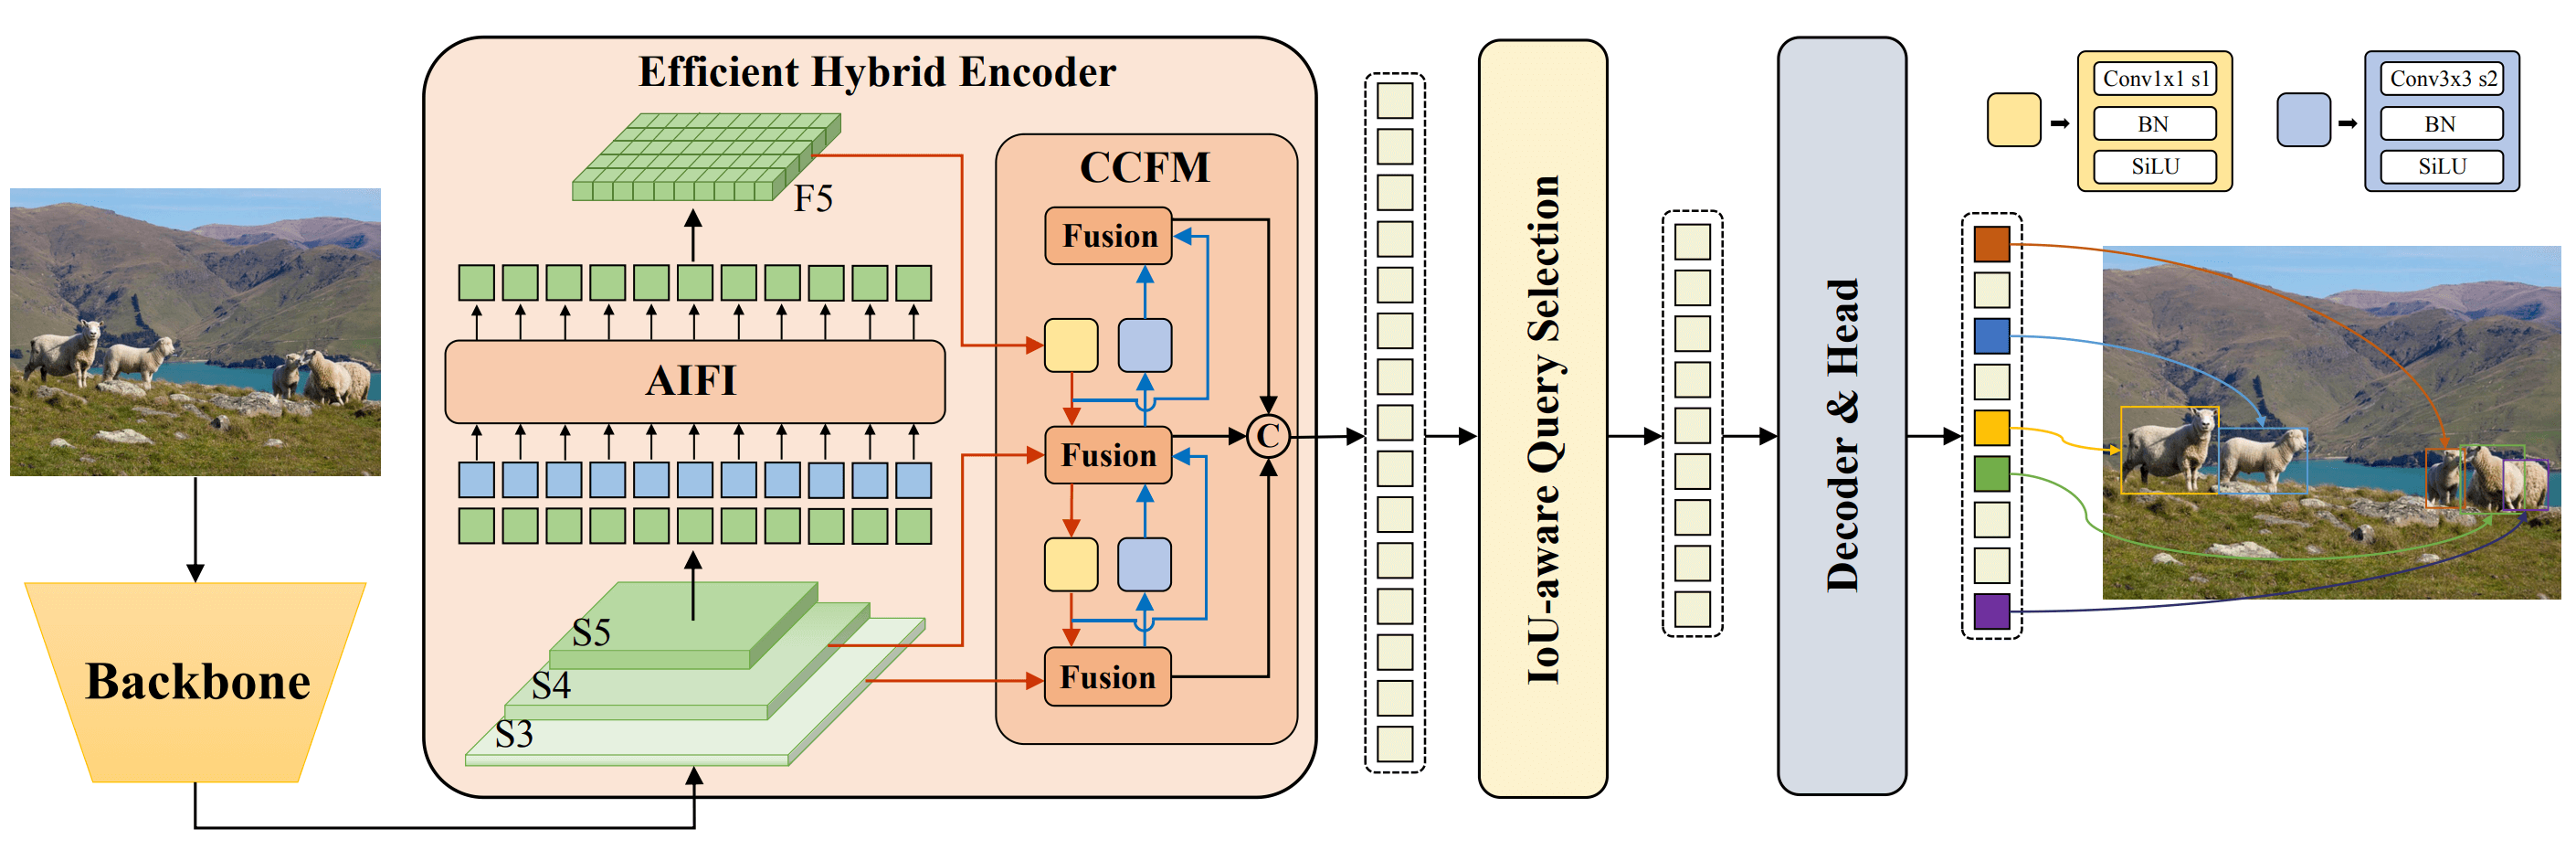
\includegraphics[scale=0.15]{images/RT-DETR.png}
    \caption{RT-DETR architecture.}
    \label{fig:RT-DETR_architecture}
\end{figure}

Another distinctive component is the \textbf{uncertainty-minimal query selection} strategy proposed to initialize the decoder with higher-quality object queries \cite{zhao_detrs_2024}. Rather than forwarding a large set of generic queries, RT-DETR selects encoder features that are expected to be more reliable starting points for detection. Intuitively, the model favors features that are informative both for object classification and for localization, so that the decoder begins its refinement process from more promising candidate regions. This improves efficiency and contributes to stronger detection accuracy.

This query selection mechanism should not be interpreted as a simple hand-crafted thresholding rule, such as selecting all predictions above a fixed IoU value. Instead, it is part of the learned initialization process of the detector and is designed to provide the decoder with a compact set of high-quality queries. After this initialization, the decoder iteratively refines the selected queries into final predictions.

In addition, RT-DETR retains the one-to-one matching paradigm based on the \textbf{Hungarian algorithm}, ensuring that each predicted object is assigned to at most one ground-truth instance during training. This bipartite matching mechanism is central to DETR-style detectors because it removes duplicate assignments and enables an end-to-end detection pipeline without NMS \cite{zhao_detrs_2024}.
\begin{figure}[h]
    \centering
    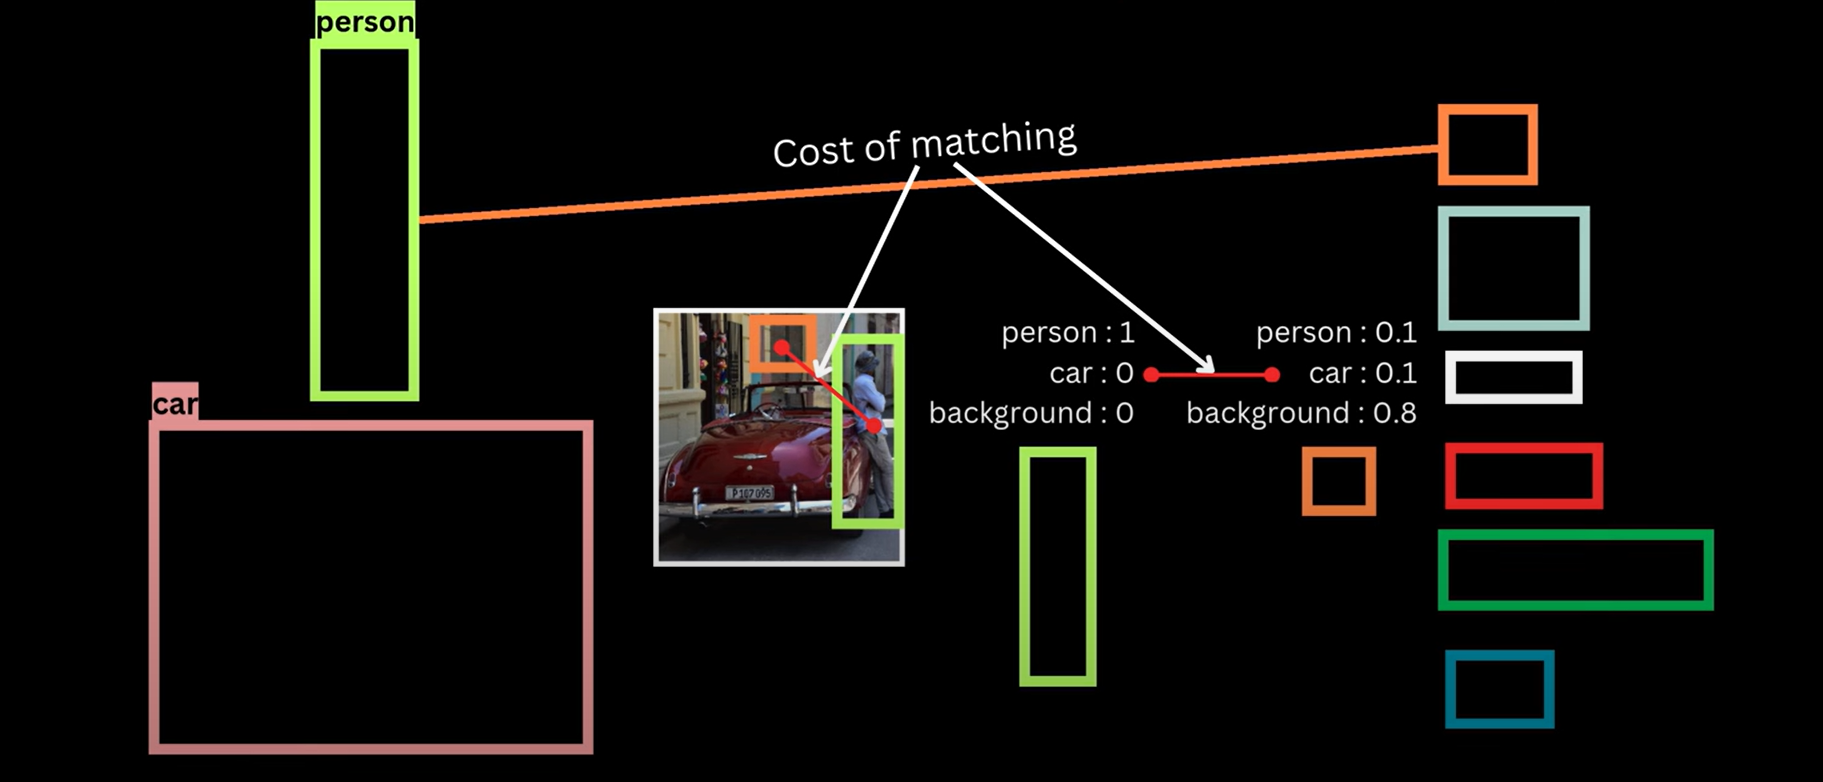
\includegraphics[scale=0.2]{images/Hungarian_match.png}
    \caption{Hungarian matching in RT-DETR.}
    \label{fig:Hungarian_match}
\end{figure}

An additional practical advantage of RT-DETR is its \textbf{flexible speed tuning}: the inference speed can be adjusted by varying the number of decoder layers, allowing the model to adapt to different deployment constraints without retraining \cite{zhao_detrs_2024}. Overall, RT-DETR achieves a strong balance between detection accuracy and computational efficiency, making transformer-based object detection more compatible with real-time and resource-constrained applications. In the context of this thesis, RT-DETR is particularly relevant because it shows how transformer principles can be adapted from generic vision representation learning to an efficient end-to-end detector, while also providing the conceptual basis for subsequent models such as DEIMv2.

\section{Related work}
% !TeX root = ../../tesi.tex

Before selecting the model to be deployed in the proposed inspection pipeline, a comparative literature study was conducted to identify the SOTA architecture that best matched the requirements of this thesis. The analysis focused on three candidate directions: a state-of-the-art real-time detector based on the DETR family (DEIMv2), an attention-centric evolution of the YOLO framework (YOLOv12), and a recent Vision-Transformer-based segmentation model (EoMT). The comparison was guided not only by reported benchmark accuracy, but also by computational cost, parameter efficiency, scalability across hardware regimes, and overall suitability for real-time deployment in the industrial scenarios considered in this work.

\subsection{DEIMv2}
% !TeX root = ../../tesi.tex

DEIMv2 was considered the most direct candidate for this thesis because it explicitly targets the same design space of interest: high-accuracy \emph{real-time} object detection under practical computational constraints \cite{huang_real-time_2026}. Architecturally, DEIMv2 extends the RT-DETR family by combining an end-to-end transformer-based detector with \textbf{stronger backbone features}. 
It offers many variants that span a wide range of model sizes and computational budgets, making it a versatile choice for comparative evaluation. Specifically:
\begin{itemize}
    \item For the mainstream variants (S, M, L, X), it adopts \textbf{DINOv3-pretrained} or distilled Vision Transformer backbones and introduces a \textbf{\emph{Spatial Tuning Adapter} (STA)} to transform the single-scale ViT output into multi-scale features suitable for detection. 

    \item For the ultra-lightweight variants (atto, femto, pico, nano), it instead relies on pruned \textbf{HGNetv2} backbones, thereby covering GPU, edge, and mobile deployment scenarios within the same design family \cite{huang_real-time_2026}.
\end{itemize}
\begin{figure}[h]
    \centering
    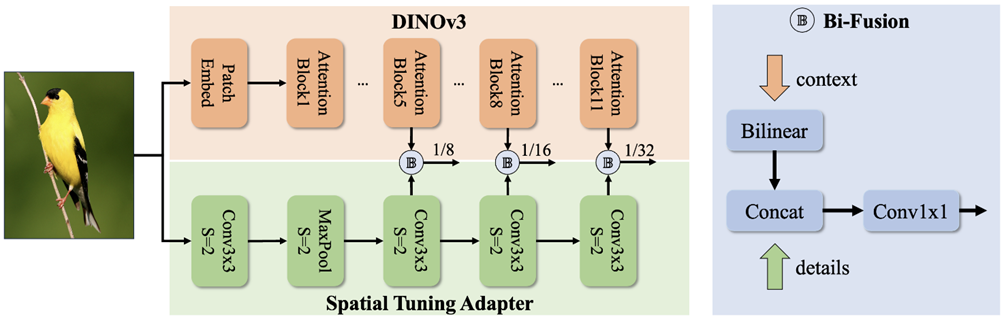
\includegraphics[width=0.8\textwidth]{images/DEIMv2.png}
    \caption{DEIMv2 architecture overview, illustrating the use of DINOv3 backbones and the Spatial Tuning Adapter (STA) to produce multi-scale features for detection \cite{huang_real-time_2026}.}
    \label{fig:DEIMv2_architecture}
\end{figure}

From the perspective of the present application, the main strength of DEIMv2 lies in its ability to combine rich semantic representations with fine-grained local details by integrating DINOv3-based features into an RT-DETR-derived detection framework. This aspect is particularly attractive for the inspection tasks considered in the thesis, since the relevant visual cues may include both global shape information and localized appearance variations. Moreover, DEIMv2 preserves the end-to-end advantages inherited from RT-DETR, including NMS-free prediction, while improving the performance--cost trade-off through stronger features, a simplified decoder, and improved training strategies such as Copy-Blend augmentation \cite{huang_real-time_2026}. The model is also highly scalable: the paper reports strong performance not only for the largest variants, but also for compact versions designed for resource-constrained deployment.
\begin{figure}[h]
    \centering
    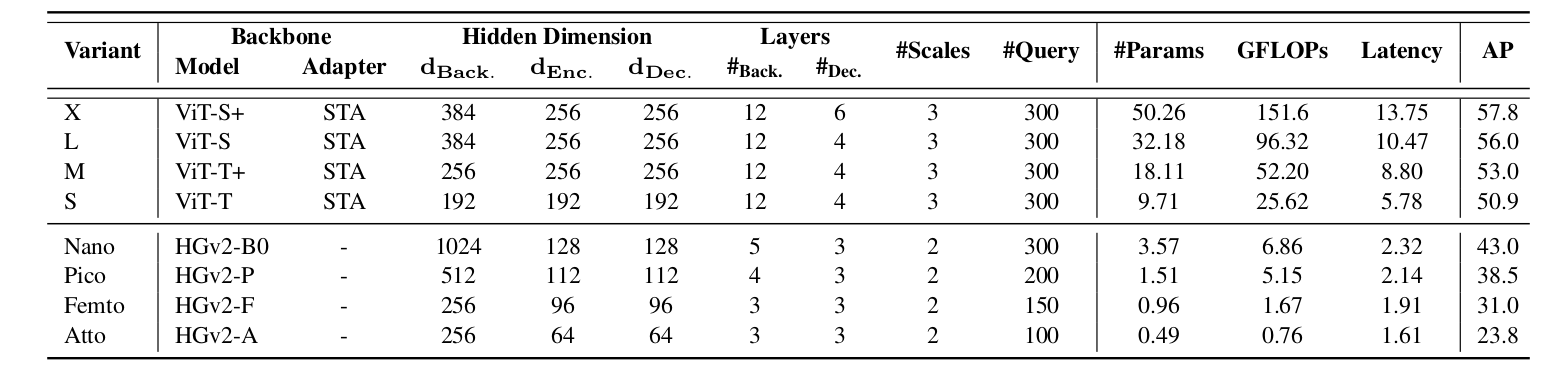
\includegraphics[width=0.9\textwidth]{images/DEIM_results.png}
    \caption{Summary of DEIMv2 results across model scales, highlighting the balance between detection accuracy, latency, and parameter efficiency \cite{huang_real-time_2026}.}
    \label{fig:DEIMv2_results}
\end{figure}

The main limitation of DEIMv2 is that part of its performance advantage depends on the availability of powerful pretrained backbones, especially for the larger variants. In other words, the strongest configurations benefit from large-scale representation learning prior to the downstream detection task. Even so, the model remains particularly compelling within the present comparative study because it combines strong reported accuracy, broad scalability, and clear compatibility with real-time detection requirements \cite{huang_real-time_2026,zhao_detrs_2024}.

\subsection{YOLOv12}
% !TeX root = ../../tesi.tex

YOLOv12 was selected as the main alternative detector because it represents a different and highly competitive design philosophy for real-time object detection \cite{tian_yolov12_2025}. Instead of building on the DETR lineage, YOLOv12 revisits the YOLO framework by introducing an \textbf{\emph{attention-centric}} architecture. Its core idea is to integrate the modeling strength of attention mechanisms into a real-time detector without sacrificing the low-latency behavior that has traditionally made YOLO models attractive in industrial settings. To do so, the paper \cite{tian_yolov12_2025} introduces three key elements: 
\begin{itemize}
    \item \textbf{Area Attention}: A novel attention mechanism that reduces the computational cost of attention by grouping spatial locations into areas, allowing the model to capture long-range dependencies with fewer computations (Figure \ref{fig:YOLOv12_attention}).
    \begin{figure}[h]
        \centering
        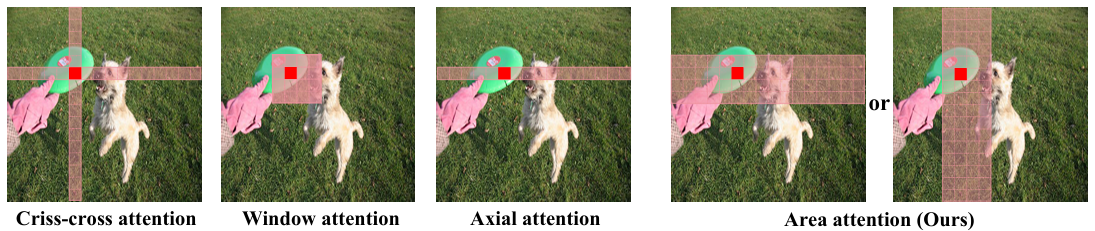
\includegraphics[width=0.9\textwidth]{images/YOLO1.png}
        \caption{Area attention mechanism in YOLOv12 compared to traditional attention mechanisms.}
        \label{fig:YOLOv12_attention}
    \end{figure}
    \item \textbf{R-ELAN}: A modified version of the ELAN architecture that improves optimization stability and convergence in deeper attention-based models, enabling YOLOv12 to scale effectively (Figure \ref{fig:YOLOv12_R-ELAN}).
    \begin{figure}[h]
        \centering
        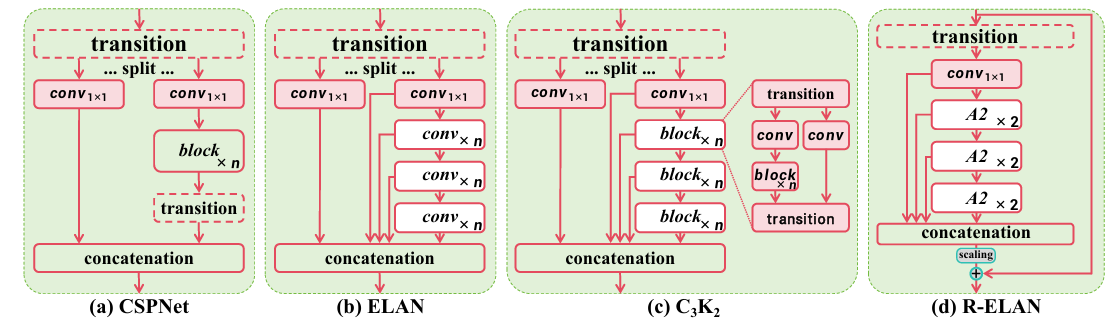
\includegraphics[width=0.9\textwidth]{images/YOLO2.png}
        \caption{YOLOv12 R-ELAN architecture overview, illustrating the skip connection mechanism to improve optimization stability in deeper attention-based models \cite{tian_yolov12_2025}.}
        \label{fig:YOLOv12_R-ELAN}
    \end{figure}
    \item \textbf{FlashAttention}: An efficient implementation of attention that reduces memory-access overhead during inference, further contributing to YOLOv12's low latency.
\end{itemize}

The main appeal of YOLOv12 in the context of this thesis is its excellent latency--accuracy trade-off and its ability to achieve strong results without depending on additional large-scale pretraining strategies. This makes it an attractive candidate whenever extremely low inference time is the primary design criterion. In addition, YOLOv12 is conceptually important because it shows that attention mechanisms can be integrated effectively even within the traditionally convolution-centric YOLO family, thereby challenging the assumption that attention is necessarily too slow for real-time detection \cite{tian_yolov12_2025}.

At the same time, YOLOv12 presents some practical limitations for the specific selection process carried out in this thesis. Its efficiency gains partly depend on hardware support for FlashAttention, which is not equally available across all deployment environments. Furthermore, according to the comparative evidence discussed in the DEIMv2 paper, DEIMv2 later surpassed YOLOv12 in the performance--cost trade-off, achieving higher detection accuracy with fewer parameters and lower computational cost in corresponding regimes \cite{huang_real-time_2026,tian_yolov12_2025}, as showed in Figure \ref{fig:DEIMvsYOLO}. For this reason, YOLOv12 was regarded as a strong benchmark and a valuable reference point, but not as the final choice for deployment.
\begin{figure}[h]
    \centering
    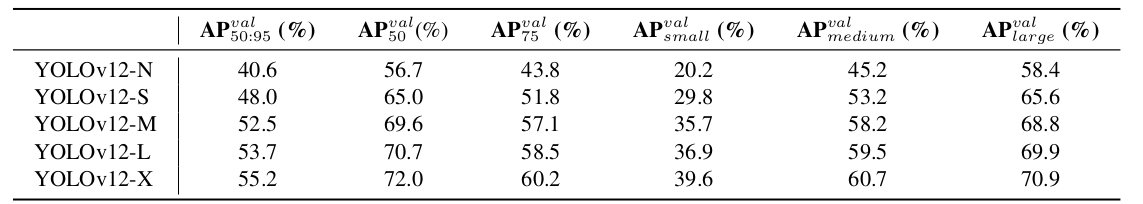
\includegraphics[width=0.9\textwidth]{images/YOLO_results.png}
    \caption{Summary of YOLOv12 results on the COCO benchmark, highlighting its strong balance between detection accuracy and inference efficiency across model scales \cite{tian_yolov12_2025}.}
    \label{fig:YOLOv12_Results}
\end{figure}

\subsection{EoMT}
% !TeX root = ../../tesi.tex

The third candidate direction explored in the literature study was not a detector, but a recent Vision-Transformer-based segmentation model, namely the Encoder-only Mask Transformer (EoMT), introduced in \emph{Your ViT is Secretly an Image Segmentation Model} \cite{kerssies_your_2025}. This work is particularly relevant because it addresses a dense prediction problem that is closely related to object localization, while doing so with a design philosophy aligned with the transformer-based trend discussed in the previous sections. The central idea of EoMT is that, given sufficiently large ViTs and sufficiently strong pretraining, many task-specific segmentation components become less necessary. For this reason, the model removes the convolutional adapter, the pixel decoder, and the separate transformer decoder typically used in ViT-based segmentation pipelines, and replaces them with a simpler encoder-only design augmented by learnable queries and a lightweight mask prediction module \cite{kerssies_your_2025}.

This approach offers several attractive properties. First, it substantially simplifies the segmentation architecture while retaining competitive accuracy. Second, by progressively removing masked attention during training through a \emph{mask annealing} strategy, EoMT enables significantly faster inference than more complex ViT-based segmentation systems. Third, because it stays close to the plain ViT architecture, it can directly benefit from future improvements in large-scale pretraining and transformer optimization \cite{kerssies_your_2025}. From a research standpoint, EoMT was therefore an appealing candidate because it suggested a potentially elegant route toward precise object delineation.

However, the comparative study also highlighted an important mismatch with the main requirements of this thesis. The thesis pipeline ultimately requires robust and efficient \emph{object localization} on embedded or edge-oriented hardware, whereas EoMT is designed for segmentation benchmarks and derives much of its strength from large pretrained ViTs and high-throughput inference settings \cite{kerssies_your_2025}. Although segmentation can provide richer pixel-level information, that additional output is not strictly necessary for the core deployment objective considered here, namely fast localization of dough balls and bread loaves prior to subsequent processing stages. Consequently, EoMT was considered highly interesting from a methodological perspective, but less aligned than DEIMv2 with the operational constraints and output requirements of the thesis.

\subsection{Final considerations}
% !TeX root = ../../tesi.tex

The comparative analysis of the three candidate families revealed a common trend: modern vision systems are increasingly moving beyond purely convolutional designs and are exploiting transformer-based representations in progressively more effective ways. Nevertheless, the final choice could not be based on architectural novelty alone. It had to reflect the concrete needs of the thesis, namely accurate and real-time localization of products in industrial environments, compatibility with edge-oriented deployment, and a favorable balance between predictive performance and computational cost.

Within this framework, DEIMv2 emerged as the most suitable solution. Compared with YOLOv12, it offered a more favorable overall performance--cost trade-off according to the evidence reported in the literature, combining higher detection accuracy with competitive or lower parameter and FLOP budgets in the corresponding model regimes, as illustrated in Figure~\ref{fig:DEIMvsYOLO} \cite{huang_real-time_2026,tian_yolov12_2025}. In addition, its integration of DINOv3-based representations and multi-scale adaptation made it particularly appealing for scenarios in which both local visual details and more global semantic structure may contribute to robust object detection.
Furthermore, DEIMv2's variety of model sizes and its compatibility with real-time detection requirements made it a versatile choice for the different deployment scenarios considered in the thesis, ranging from GPU-based inference to edge-oriented applications \cite{huang_real-time_2026,zhao_detrs_2024}. By contrast, part of YOLOv12's efficiency advantage depends on hardware support for FlashAttention, which is not uniformly available across all deployment environments. In this respect, DEIMv2 appears more flexible and robust as a practical choice for heterogeneous hardware settings.
\begin{figure}[h]
    \centering
    \captionsetup[subfigure]{justification=centering}
    \begin{subfigure}[t]{0.48\textwidth}
        \centering
        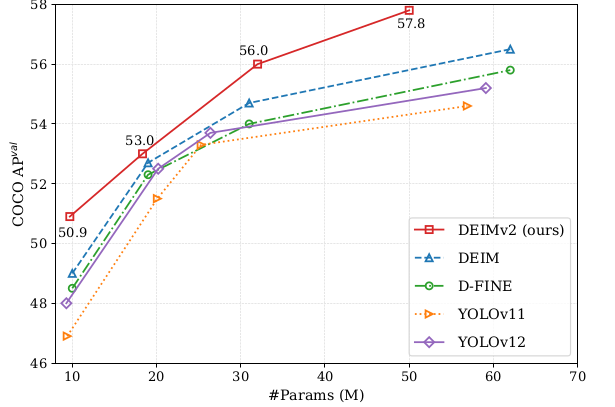
\includegraphics[width=\textwidth]{images/DEIMvsYOLO1.png}
        \caption[c]{Accuracy versus number of parameters for DEIMv2 and YOLOv12 across model scales \cite{huang_real-time_2026,tian_yolov12_2025}.}
        \label{fig:DEIMvsYOLO1}    
    \end{subfigure}\hfill
    \begin{subfigure}[t]{0.48\textwidth}
        \centering
        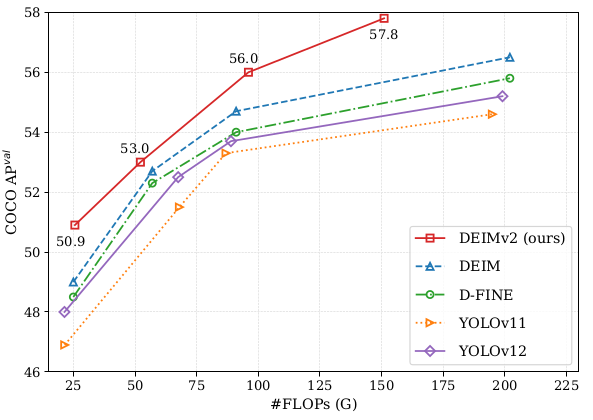
\includegraphics[width=\textwidth]{images/DEIMvsYOLO2.png}
        \caption[c]{Accuracy versus computational cost for DEIMv2 and YOLOv12 across model scales \cite{huang_real-time_2026,tian_yolov12_2025}.}
        \label{fig:DEIMvsYOLO2}
    \end{subfigure}
    \caption{Comparison between DEIMv2 and YOLOv12 in terms of accuracy, parameter count, and computational cost, highlighting the stronger overall efficiency of DEIMv2 across the considered model scales \cite{huang_real-time_2026,tian_yolov12_2025}.}
    \label{fig:DEIMvsYOLO}
\end{figure}

The comparison with EoMT requires a different interpretation, because EoMT addresses image segmentation rather than object detection. For this reason, the decisive argument was not that DEIMv2 is universally superior on a common benchmark, but that it is better aligned with the objective of the thesis. In the proposed pipeline, the essential requirement is to localize each dough ball or loaf quickly and reliably, so that subsequent modules can estimate geometric or appearance-based quantities. For this thesis, object detection is therefore the more appropriate output representation: a full segmentation model would provide richer pixel-level information, but at the cost of denser prediction, greater architectural complexity, and weaker compatibility with low-latency embedded deployment. Moreover, the advantages of EoMT are most evident when large pretrained ViTs and high-performance hardware are available, whereas the thesis prioritizes an efficient real-time detector that can be deployed in practical industrial settings \cite{kerssies_your_2025}.

For these reasons, DEIMv2 was selected as the detection model adopted in this thesis. It combines state-of-the-art real-time detection performance, strong scalability across model sizes, and a transformer-based design that remains compatible with the broader evolution of modern vision architectures. At the same time, the study of YOLOv12 and EoMT remained valuable: YOLOv12 highlighted the growing viability of attention-centric real-time detectors, while EoMT showed that large pretrained ViTs can increasingly absorb task-specific dense prediction components. Together, these works provided the conceptual background against which DEIMv2 was identified as the most appropriate choice for this thesis.

\section{Anomaly Detection}
Anomaly detection is the task of identifying samples that deviate significantly from the expected distribution of normal data. In computer vision, this usually means detecting images or regions whose appearance is inconsistent with the visual patterns observed during training. In industrial inspection, anomaly detection is particularly relevant because defective samples are often rare, heterogeneous, and difficult to collect in a representative way.\cite{li_survey_2025}

Depending on the formulation, visual anomaly detection may operate at different levels of granularity. Some methods produce an \textbf{image-level anomaly score}, indicating whether an image is normal or abnormal as a whole, while others also provide a \textbf{pixel-level anomaly map} that localizes suspicious regions. This distinction is important in industrial settings, where both the decision itself and the interpretability of the detected defect can be relevant.\cite{li_survey_2025}

A common scenario in industrial practice is that abundant normal samples are available, whereas anomalous examples are scarce or completely unavailable. For this reason, many modern anomaly detection methods are designed to learn only the distribution of normal data and to treat deviations from that distribution as potential anomalies.\cite{li_survey_2025} This setting is especially attractive when defects are difficult to enumerate in advance or when collecting defective products would be impractical.

From a methodological perspective, deep-learning-based anomaly detection methods can be grouped into several broad families, including reconstruction-based approaches, feature-embedding methods, teacher--student models, memory-bank methods, and hybrid approaches.\cite{li_survey_2025} Although these methods differ in architecture and supervision signals, they share the same central objective: building a representation of normality that makes abnormal patterns stand out at inference time.

\begin{figure}[h]
    \centering
    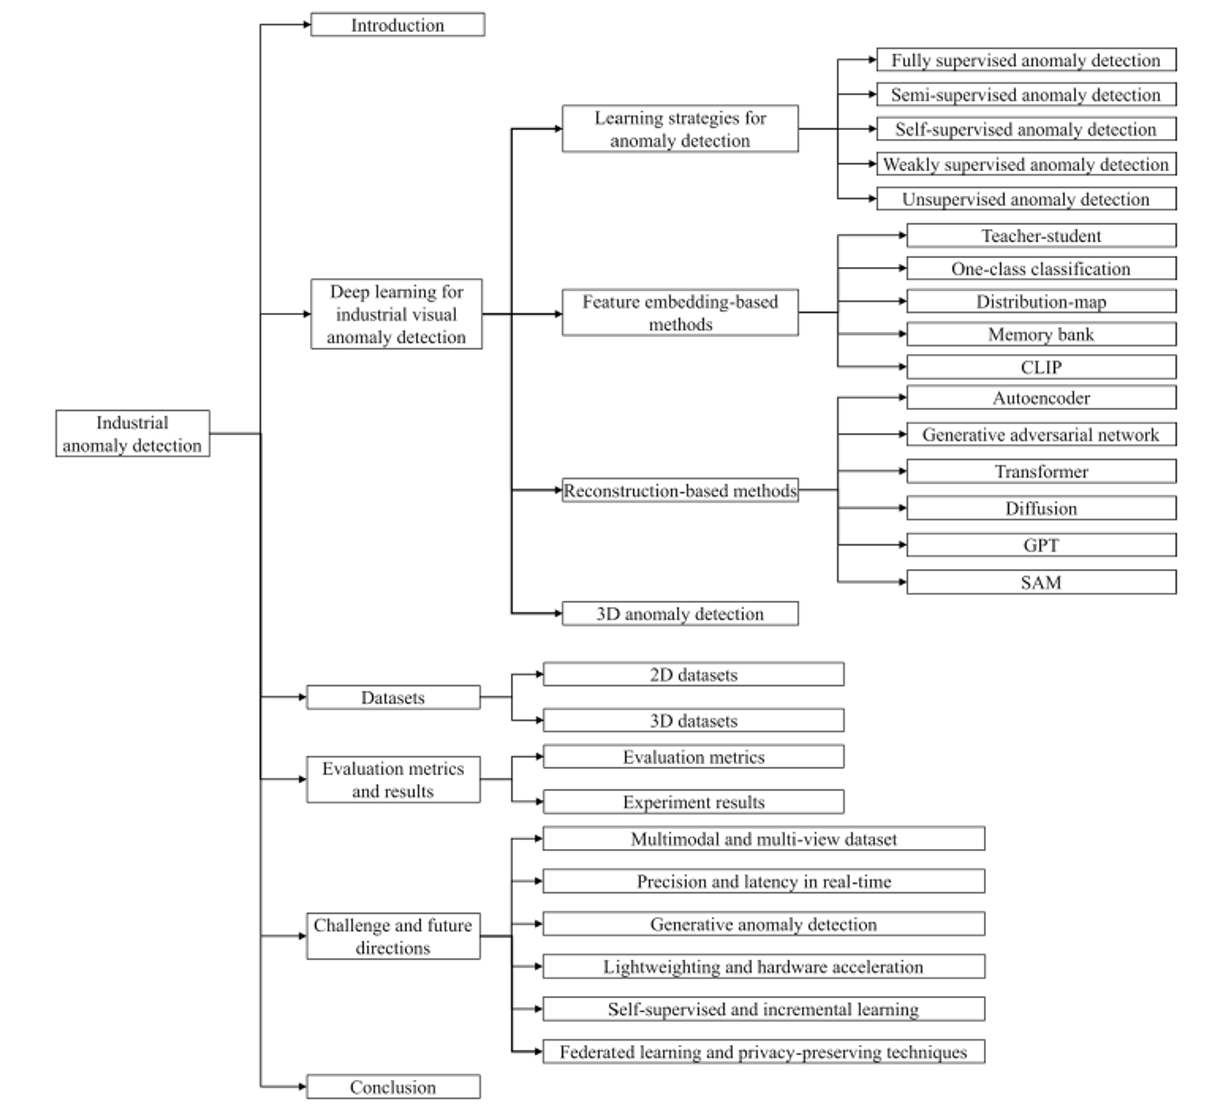
\includegraphics[width=0.9\linewidth]{images/Anomaly.png}
    \caption{Overview of the main methodological families in industrial visual anomaly detection.\cite{li_survey_2025}}
    \label{fig:ivad_taxonomy}
\end{figure}

\subsection{EfficientAD}
Among the anomaly detection methods considered for this thesis, \textbf{EfficientAD} was particularly attractive because it was explicitly designed to achieve a favorable balance between detection accuracy and very low inference latency.\cite{batzner_efficientad_2024} This property is especially important in industrial applications, where anomaly detection must often be integrated into real-time or near-real-time processing pipelines.

At a high level, EfficientAD follows a \textbf{teacher--student paradigm}. A teacher network extracts reference features from normal images, while a student network is trained to reproduce those features on anomaly-free data.\cite{batzner_efficientad_2024} During inference, a large discrepancy between teacher and student representations indicates that the input may contain an anomalous pattern. In addition to this feature-prediction mechanism, EfficientAD incorporates an autoencoder branch to better capture more global or logical anomalies that cannot be explained only through local feature mismatches.\cite{batzner_efficientad_2024}

\begin{figure}[h]
    \centering
    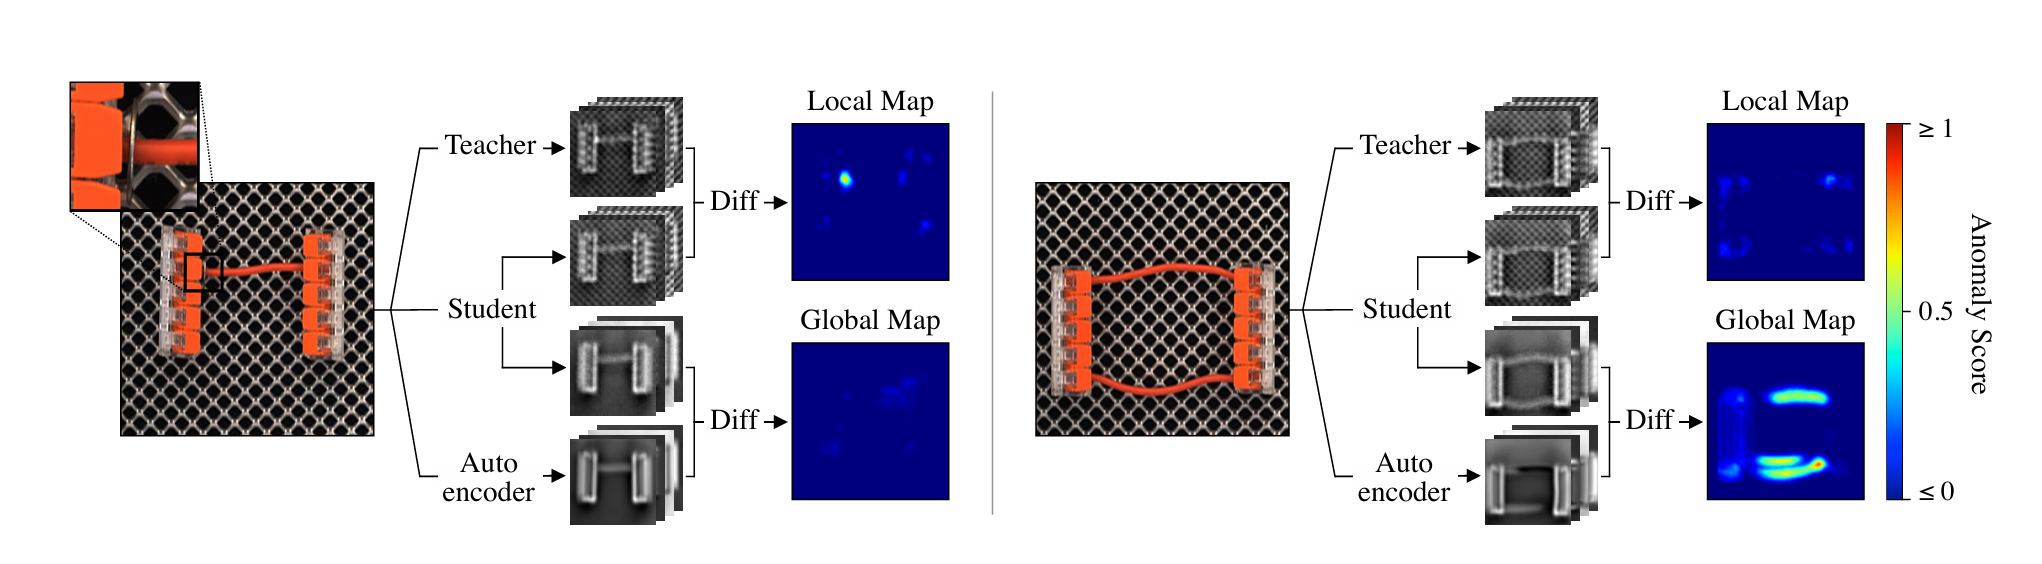
\includegraphics[width=0.95\linewidth]{images/EfficientAD_structure.png}
    \caption{EfficientAD architecture combining teacher--student feature comparison and an autoencoder branch to produce anomaly maps and an image-level anomaly score.\cite{batzner_efficientad_2024}}
    \label{fig:efficientad_architecture}
\end{figure}
\newpage
The main reason for selecting EfficientAD over other anomaly detection methods was therefore practical as well as methodological. First, it is designed for \textbf{high-speed inference}, which makes it suitable for deployment scenarios in which computational resources and response time are both important constraints.\cite{batzner_efficientad_2024} Second, it is available within the \textbf{anomalib} framework, which provides a unified and relatively straightforward implementation environment for state-of-the-art anomaly detection models.\cite{akcay_anomalib_2022} In this sense, EfficientAD offered a combination of efficiency, strong reported performance, and ease of integration that made it particularly convenient for the present work.

Another important aspect is that EfficientAD is well suited to settings in which only normal training samples are available.\cite{batzner_efficientad_2024,li_survey_2025} This makes it particularly relevant for industrial inspection problems in which anomalous data are scarce, poorly characterized, or unavailable during model development. For the purposes of this thesis, this characteristic was especially valuable, because the anomaly detection task had to be framed around learning a reliable representation of normal bread appearance and then measuring deviations from it at inference time.
\begin{figure}[h]
    \centering
    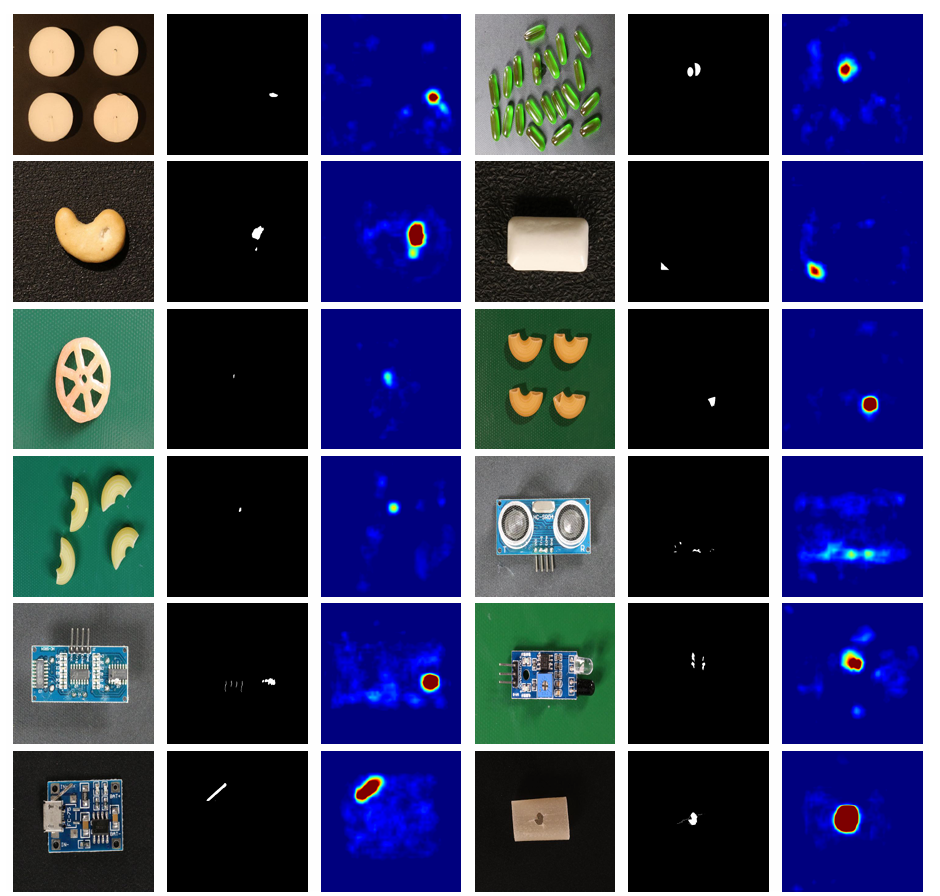
\includegraphics[width=0.6\linewidth]{images/EfficientAD_examples.png}
    \caption{Examples of EfficientAD anomaly maps. The anomalies are highlighted in red, while the normal regions are shown in blue. }
    \label{fig:efficientad_examples}
\end{figure}

\section{Training an AI}
Training a deep learning model consists of iteratively updating its parameters in order to minimize a predefined loss function on the available data.\cite{goodfellow_deep_2016} In supervised and weakly supervised settings, this optimization process is not evaluated solely on the data used for parameter updates, but also on held-out data that provide an estimate of how well the model generalizes to unseen samples.\cite{goodfellow_deep_2016}

For this reason, both the organization of the dataset and the interpretation of training dynamics are central to the development of reliable models. In particular, a clear separation between training, validation, and test data is essential for model selection, while the notions of overfitting and underfitting are fundamental for understanding whether a model is learning meaningful patterns or failing to generalize beyond the training set.\cite{goodfellow_deep_2016}

\subsection{Dataset-split}
A standard practice in machine learning is to divide the available data into at least three subsets: a training set, a validation set, and a test set.\cite{goodfellow_deep_2016} The training set is used to update the model parameters during optimization. The validation set is instead used to monitor generalization during development and to support decisions such as hyperparameter tuning, model selection, and stopping time. Finally, the test set is reserved for the final evaluation of the model and should not influence training decisions.\cite{goodfellow_deep_2016}

The rationale behind this separation is that good performance on the training set alone is not sufficient: the model must also perform well on unseen data. The validation set therefore provides an intermediate estimate of generalization quality while the model is being developed, whereas the test set is used only after the design choices have been fixed.\cite{goodfellow_deep_2016} In practical applications, the exact proportions assigned to these subsets depend on the size and structure of the dataset, and there is no universally optimal split.\cite{sklearn_train_test_split_2026} However, the underlying principle remains the same: parameter learning should be performed on one subset, model selection on another, and final assessment on a third independent subset. This approach helps to prevent overfitting to the training data and ensures that the reported performance metrics reflect the model's ability to generalize to new, unseen examples.\cite{goodfellow_deep_2016}
\begin{figure}[h]
    \centering
    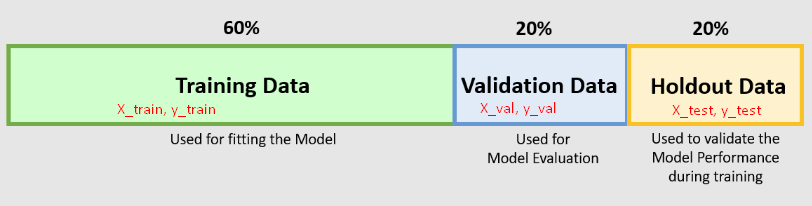
\includegraphics[width=0.85\linewidth]{images/dataset_split.png}
    \caption{Illustration of the standard partition of a dataset into training, validation, and test subsets.}
    \label{fig:dataset_split}
\end{figure}

\subsection{Overfitting-Underfitting}
Two of the central concepts in machine learning are \textbf{underfitting} and \textbf{overfitting}.\cite{goodfellow_deep_2016} Underfitting occurs when a model is unable to achieve sufficiently low error even on the training set. This usually indicates that the model is too simple, insufficiently trained, or poorly configured for the complexity of the task. Overfitting, by contrast, occurs when the model performs very well on the training data but poorly on unseen data, meaning that it has adapted too strongly to idiosyncrasies of the training set rather than learning patterns that generalize.\cite{goodfellow_deep_2016}
\begin{figure}[ht]
    \centering
    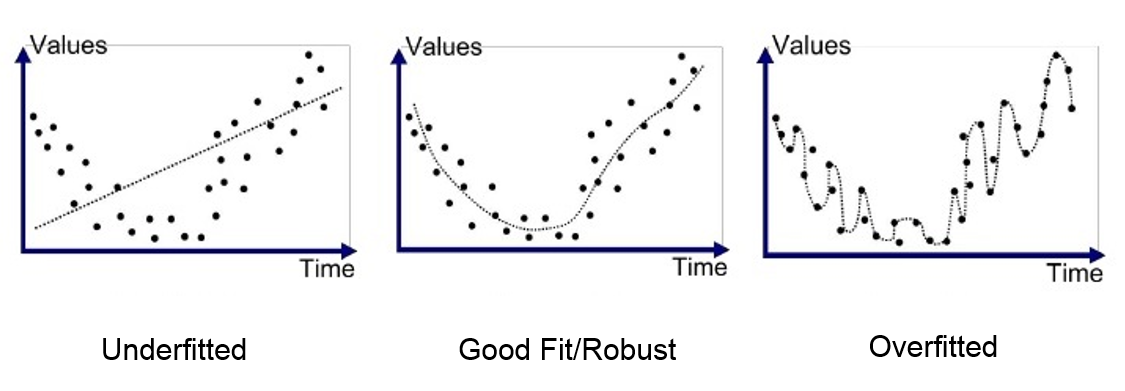
\includegraphics[width=0.75\linewidth]{images/under_over_example.png}
    \caption{Example of underfitting and overfitting in a regression task. The left plot shows an underfitting model that fails to capture the underlying trend, the middle plot shows a well-fitted model that generalizes well, and the right plot shows an overfitting model that captures noise in the training data.}
    \label{fig:example_under_overfitting}
\end{figure}

These two phenomena can often be identified through the evolution of training and validation curves. In an underfitting regime, both training and validation errors remain relatively high. In an overfitting regime, the training error keeps decreasing whereas the validation error stagnates or starts increasing. Monitoring these trends is therefore essential for understanding whether additional training is beneficial or detrimental.\cite{goodfellow_deep_2016,prechelt_early_2012}

One of the most widely used strategies for limiting overfitting is \textbf{early stopping}. During optimization, the training loss may continue to decrease even after the model has already reached its best generalization performance. When the validation error stops improving and begins to worsen, this is a signal that the model is starting to adapt too closely to the training data. Early stopping addresses this issue by interrupting training at the point of best validation performance and retaining the corresponding model parameters.\cite{goodfellow_deep_2016,prechelt_early_2012}
\begin{figure}[ht]
    \centering
    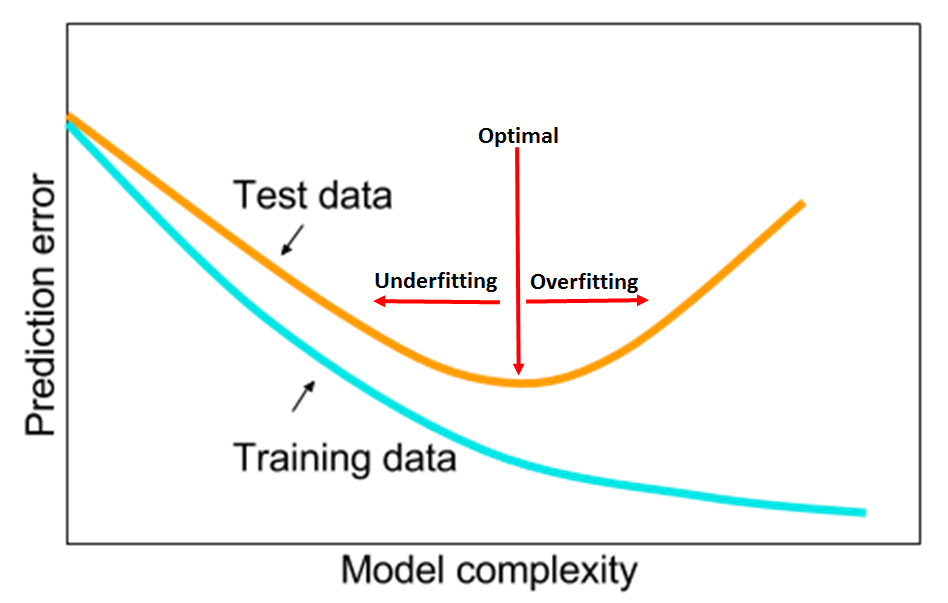
\includegraphics[width=0.6\linewidth]{images/under-overfitting.png}
    \caption{Typical training and validation behaviors in underfitting and overfitting regimes.}
    \label{fig:learning_curves_overfitting}
\end{figure}

Several strategies can be adopted to mitigate these problems. Underfitting may be addressed by increasing model capacity, improving feature quality, extending training, or refining optimization settings. Overfitting can instead be reduced through regularization techniques, data augmentation, early stopping, or, when appropriate, by simplifying the model.\cite{goodfellow_deep_2016} In practice, achieving good generalization requires balancing model capacity and training duration so that the model captures meaningful structure in the data without memorizing the training set.





 %File in cui è scritto il capitolo
\label{chapter:chapter_3} %Label per creare riferimenti al capitolo
\chapter{Data acquisition system}

\section{Site 1: dough ball production and data acquisition setup}
% !TeX root = ../../tesi.tex

Site 1 represents the first deployment environment of the proposed vision-based monitoring system. It corresponds to the production stage in which the dough exits the industrial forming machine in the form of individual cylindrical dough balls. The objective at this stage is twofold: (i) to acquire a representative RGB-D dataset for offline training of the object detection network, and (ii) to deploy the trained DEIMv2 model online in order to detect the bounding boxes corresponding to the dough balls and support volumetric estimation.
\begin{figure}[h]
    \centering
    \begin{subfigure}[h]{0.48\textwidth}
        \centering
        %\vspace{0pt}% allinea in alto
        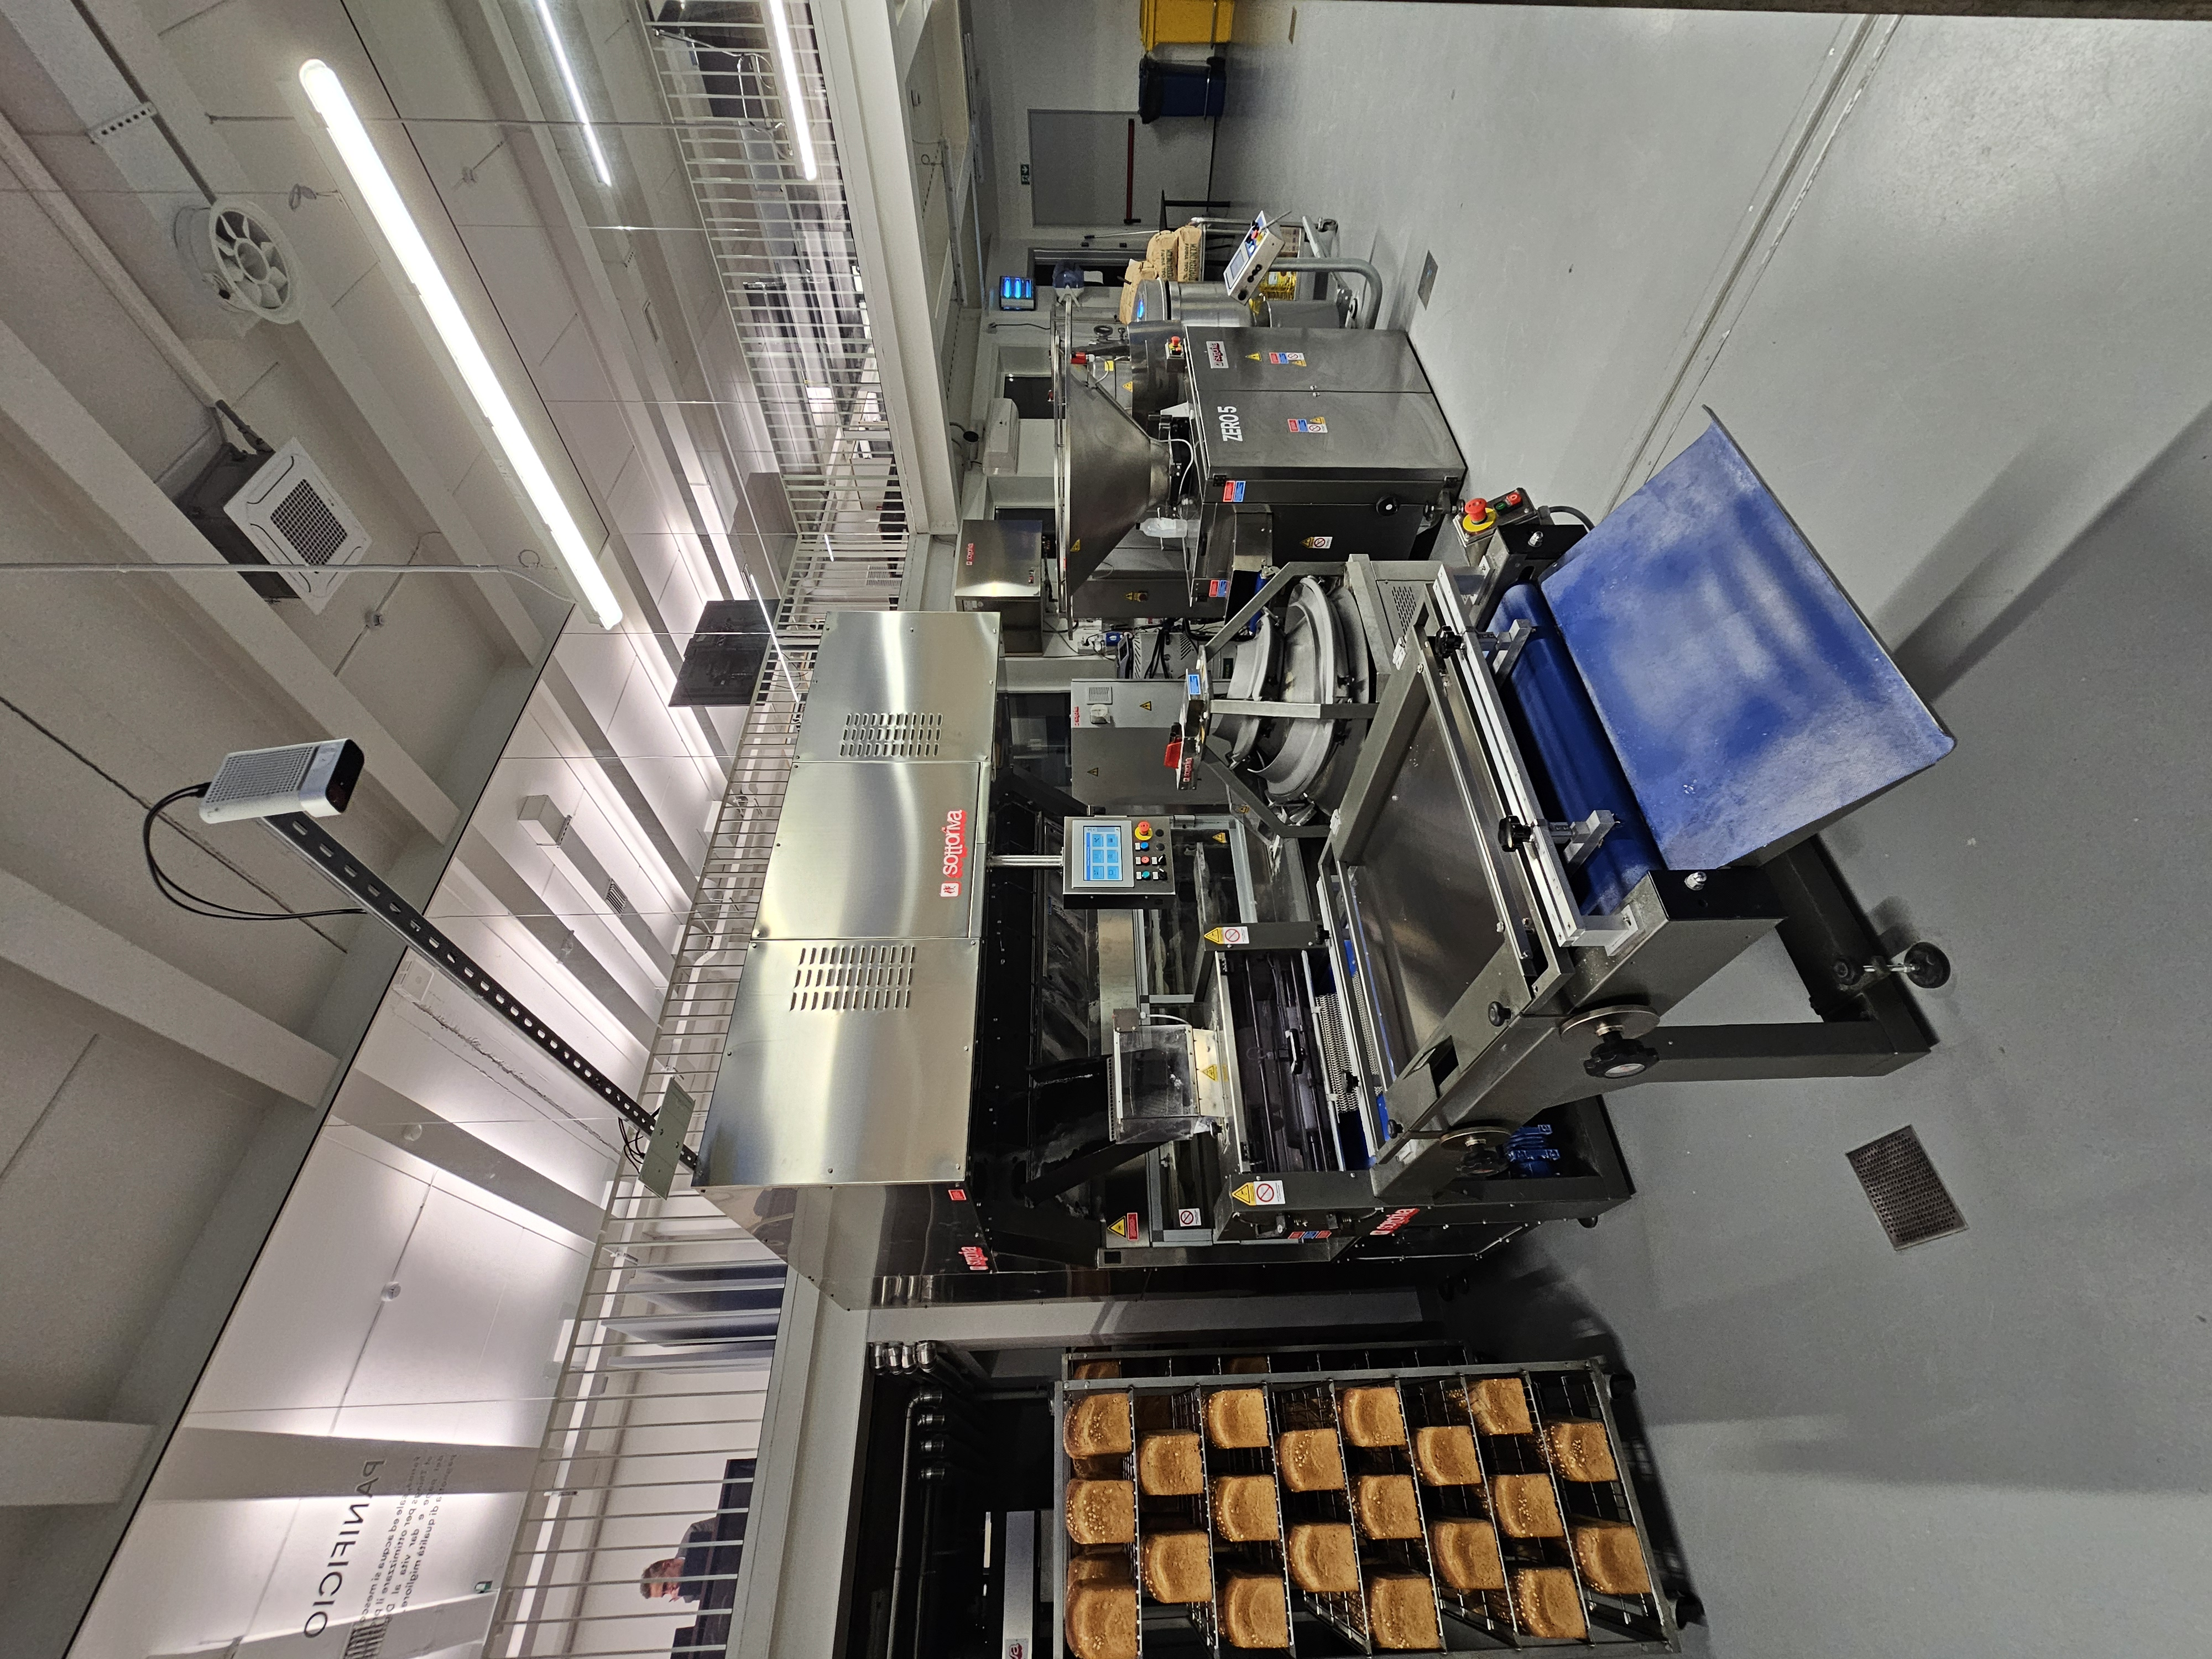
\includegraphics[scale=0.06, angle=-90, trim={0 120 120 40}, clip]{images/sito1(1).jpg}
        \caption{Automated machine pipeline at Site 1}
        \label{fig:site1_machine}
    \end{subfigure}\hfill
    \begin{subfigure}[h]{0.48\textwidth}
        \centering
        %\vspace{0pt}% allinea in alto
        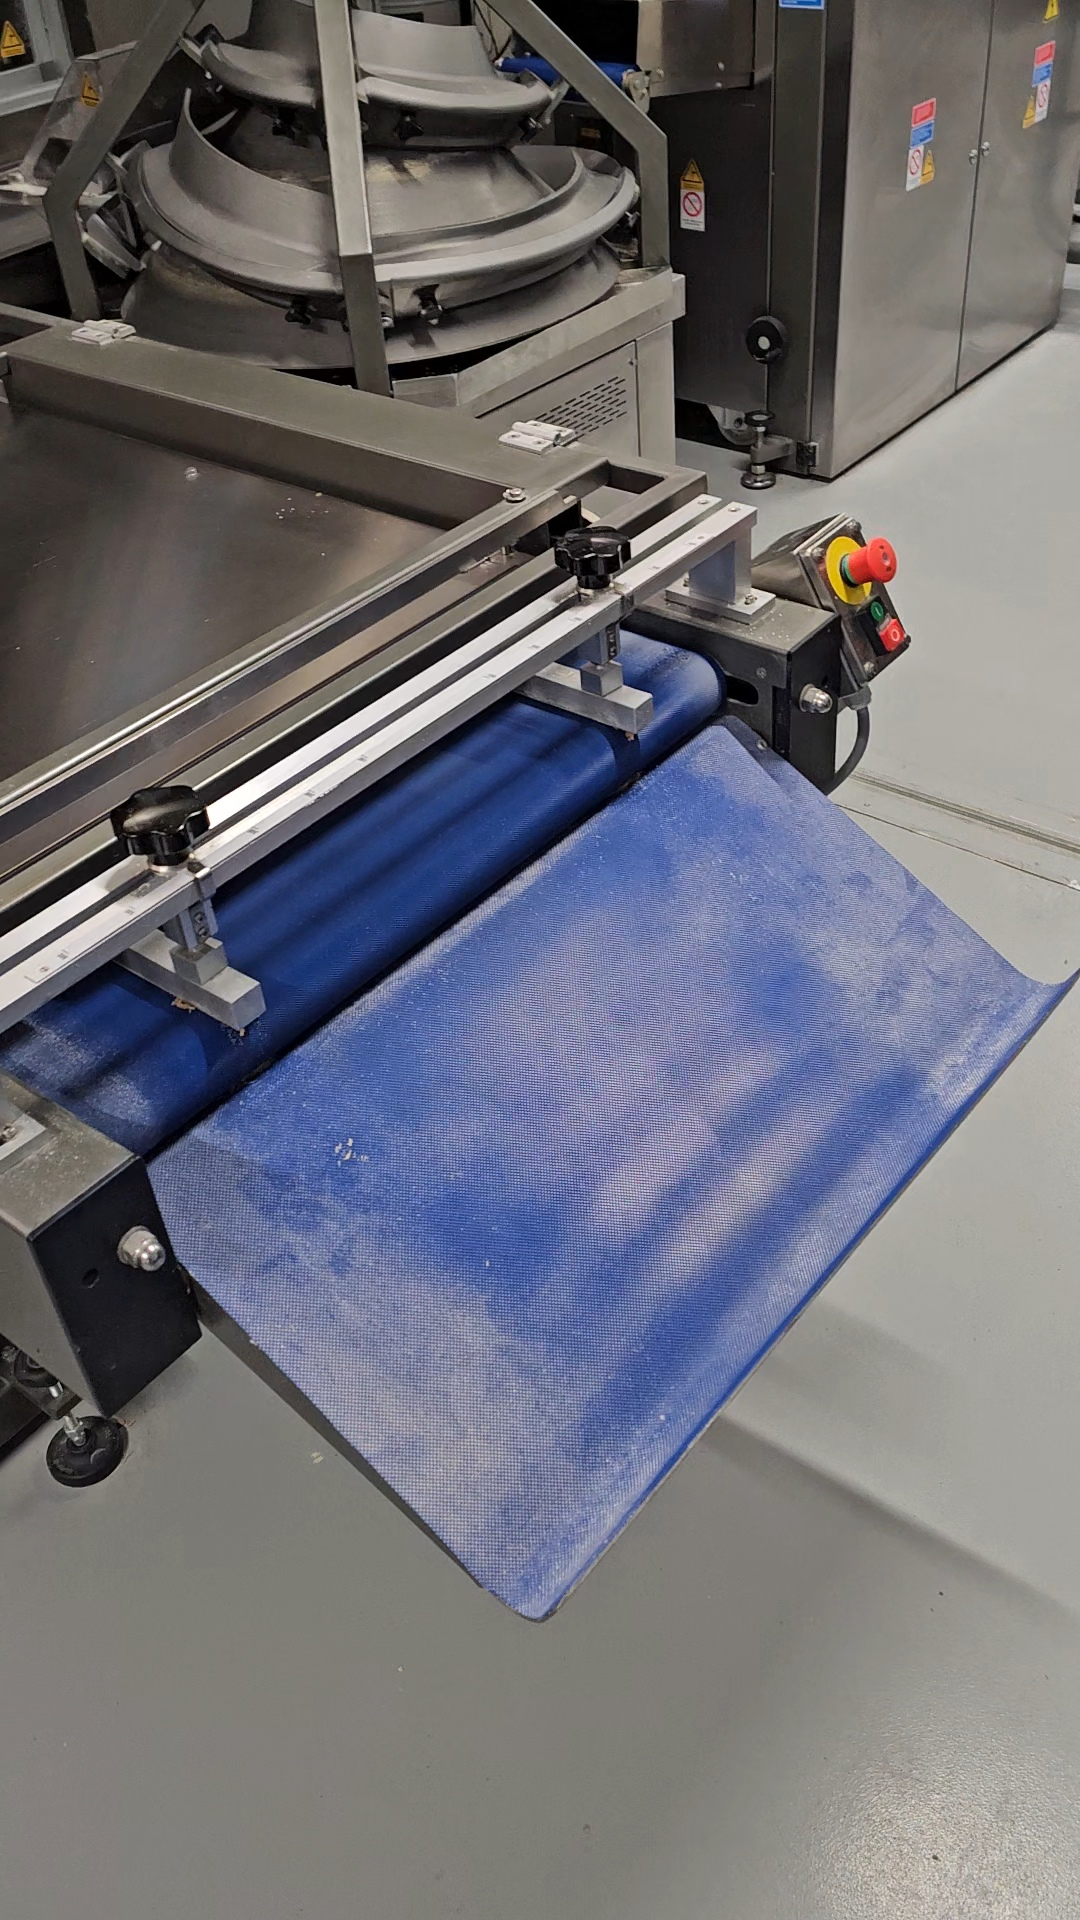
\includegraphics[scale=0.19, trim={0 280 0 400}, clip]{images/Output1-2.jpg}
        \caption{Output table where the dough balls arrive}
        \label{fig:site1_output}
    \end{subfigure}
    \caption{Overview of Site 1 and close-up of the machine output area}
    \label{fig:site1_overview}
\end{figure}
\newpage
\subsubsection{Industrial Context and Process Description}
At Site 1, the dough mixture is processed by an automated forming machine that portions and shapes the material into approximately cylindrical dough balls. These dough balls exit the machine sequentially and move along a conveyor belt until they reach the output table shown in Figure~\ref{fig:site1_output}. Variability in size and shape may occur due to fluctuations in the upstream mixing and forming processes. For quality-control purposes, it is therefore important to monitor geometric properties such as volume in a non-contact manner.

To address this requirement, a vision-based acquisition setup was installed above the machine output area, as illustrated in Figure~\ref{fig:site1_overview} and Figure~\ref{fig:hardware_site1}. The hardware configuration consists of an \emph{NVIDIA Jetson Nano 2GB Developer Kit} \cite{nvidia_corporation_jetson_nodate} for edge computation and an \emph{Azure Microsoft Kinect} RGB-D sensor \cite{microsoft_azure_nodate} for synchronized color and depth acquisition. Further details on the sensing hardware and on the Time-of-Flight principle are provided in the dedicated subsections of this chapter.

\begin{figure}[h]
    \centering
    \begin{subfigure}[h]{0.48\textwidth}
        \centering
        %\vspace{0pt}% allinea in alto
        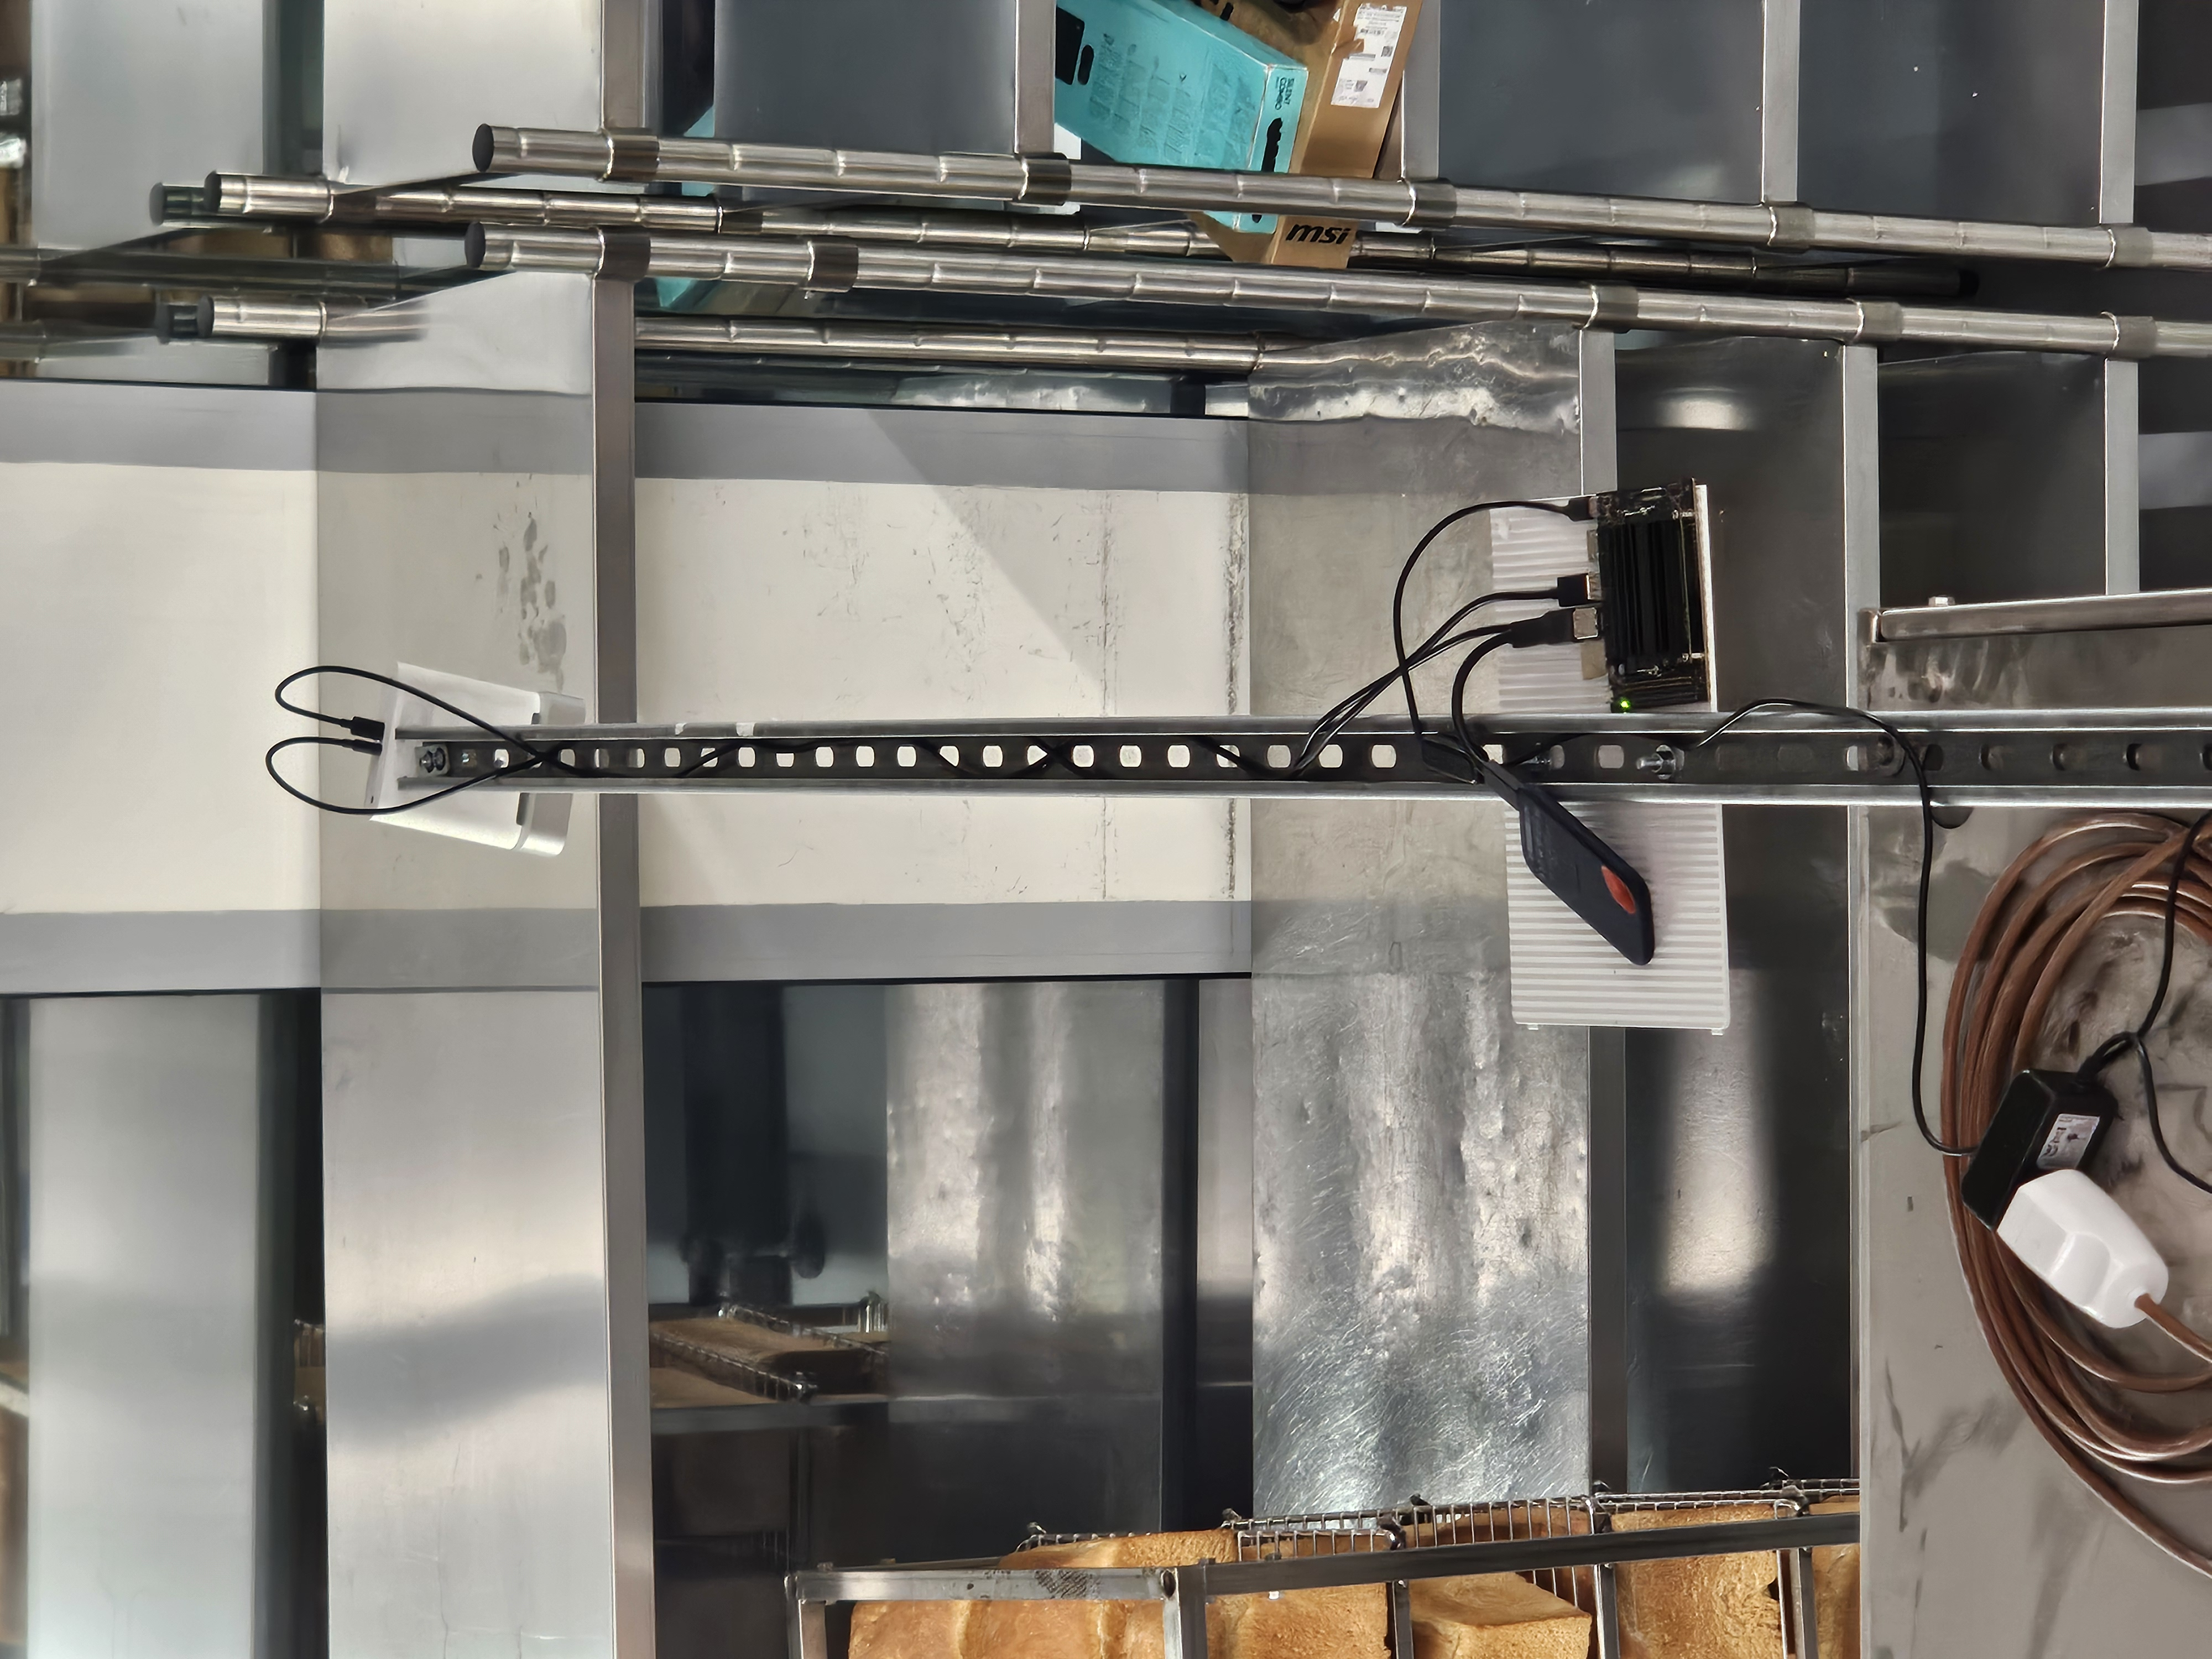
\includegraphics[width=\textwidth, angle=-90]{images/Jetson+Kinect.jpg}
        \caption{Jetson Nano and Azure Kinect used in the Site 1 setup}
    \end{subfigure}
    \begin{subfigure}[h]{0.48\textwidth}
        \centering
        %\vspace{0pt}% allinea in alto
        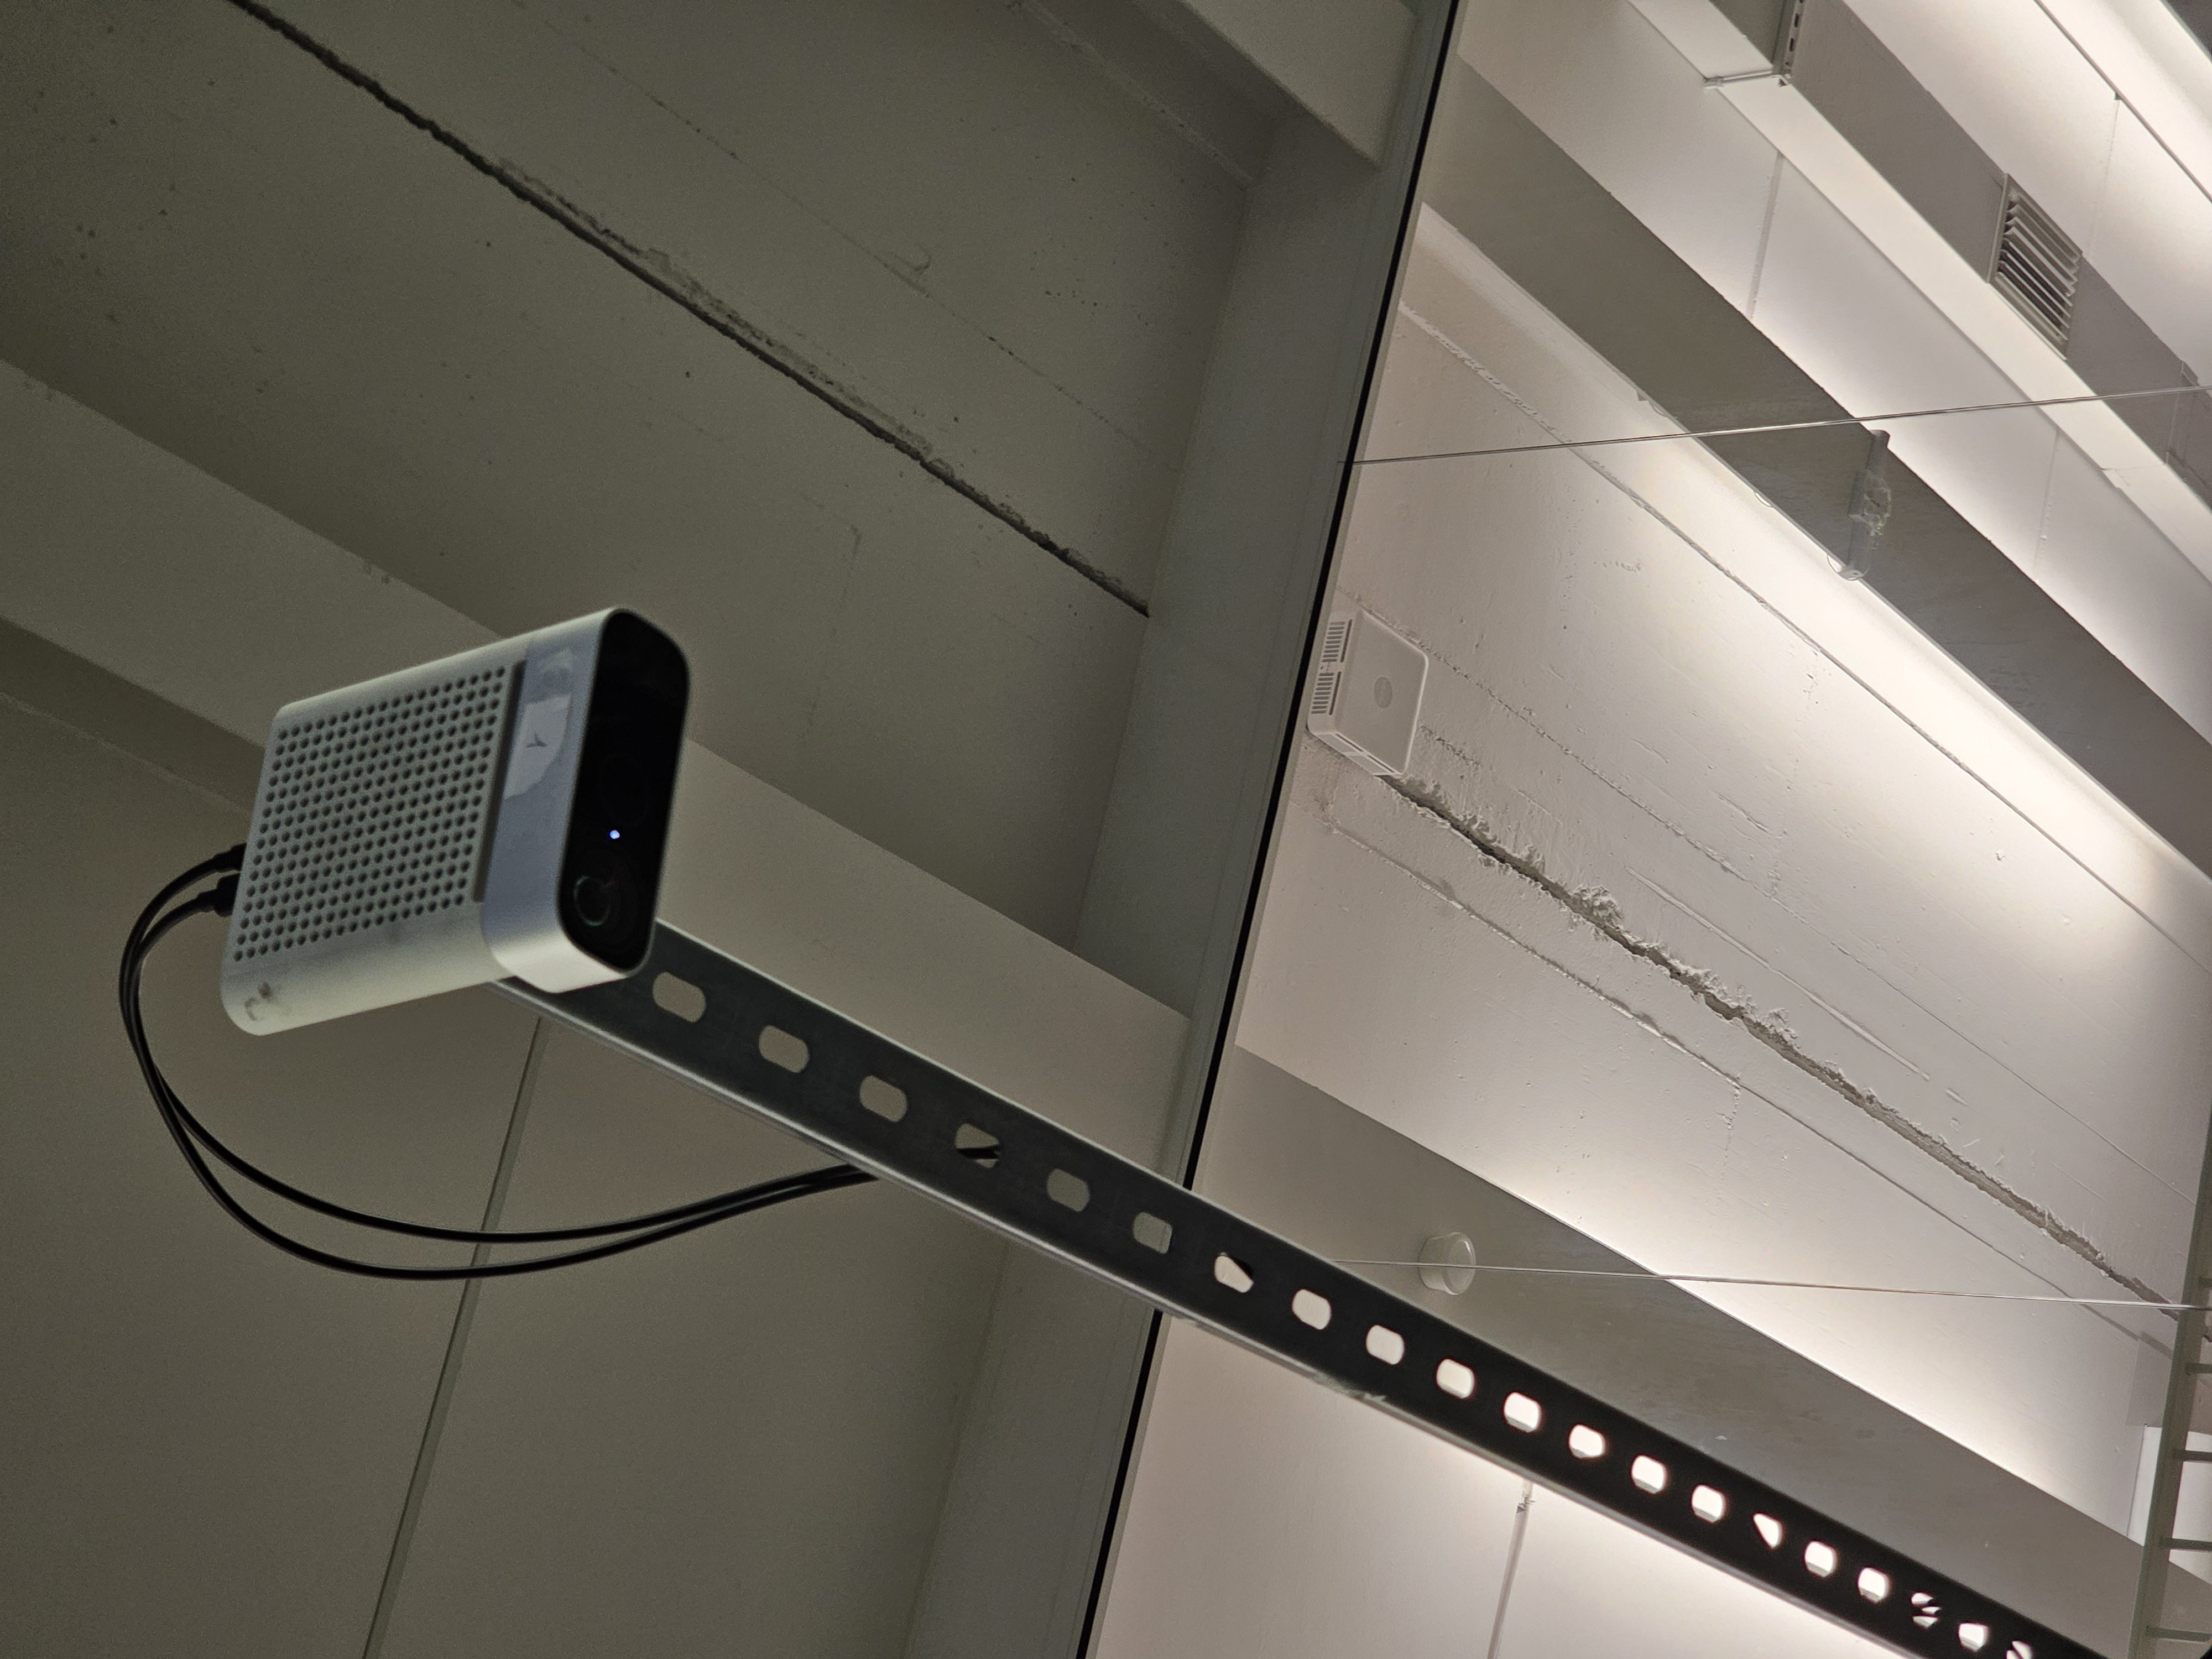
\includegraphics[width=\textwidth, angle=-90]{images/Kinect_on_site1.jpg}
        \caption{Azure Kinect mounted above the machine output area}
    \end{subfigure}
    \caption{Hardware configuration at Site 1, showing the Jetson Nano and the Azure Kinect mounted above the machine output area for RGB-D acquisition of the dough balls shown in Figure~\ref{fig:site1_output}}
    \label{fig:hardware_site1}
\end{figure}

\subsubsection{Offline Data Acquisition}
During the offline phase, the system operates in data acquisition mode. In this configuration, the Azure Kinect continuously captures synchronized RGB and depth frames. A motion detection algorithm is executed on the Jetson Nano to identify pixel variations in the scene corresponding to the passage of dough balls under the camera.

The motion detection module serves exclusively as a trigger mechanism for dataset collection. When motion is detected within a predefined and configurable region of interest (ROI), the corresponding RGB-D frame is stored. In this setup, the ROI was defined so as to cover the entire machine output area (shown in Figure~\ref{fig:site1_output}).
\newpage
This approach ensures that:
\begin{itemize}
    \item only relevant frames containing dough balls are acquired;
    \item redundant background movement is discarded;
    \item the dataset remains balanced and computationally manageable.
\end{itemize}
\begin{figure}[h]
    \centering
    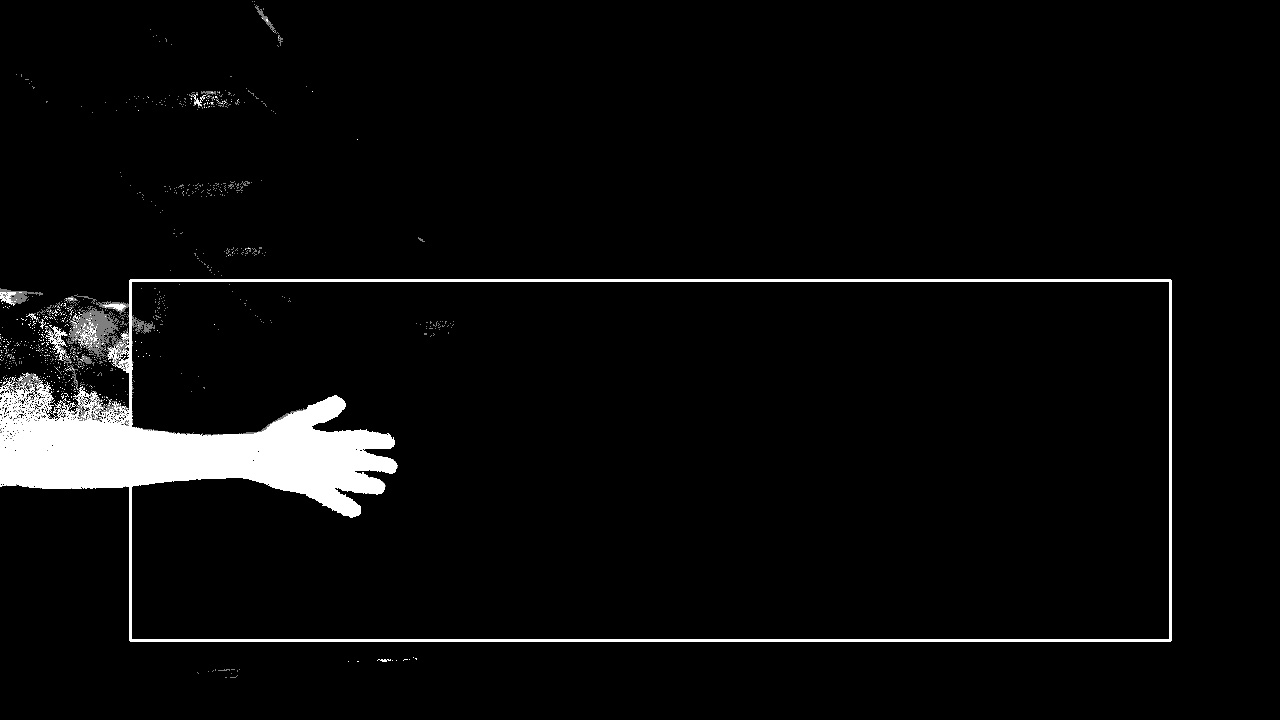
\includegraphics[width=0.65\linewidth]{images/ROI_example.jpg}
    \caption{Example of a configurable region of interest (ROI) superimposed on a background-subtraction mask. Although this example refers to the Site~2 workstation shown in Figure~\ref{fig:breadloaf}, it illustrates the same motion-triggering principle adopted for data acquisition at both sites. The white region corresponds to the detected foreground, while the black region represents the background.}
    \label{fig:acquisition_site1}
\end{figure}
The collected dataset is subsequently annotated through an automatic labelling strategy based on Language Segment-Anything \cite{medeiros_luca-medeiroslang-segment-anything_2026}, and the resulting annotations are then used to train the DEIMv2 object detection network in an offline environment. The details of the labelling procedure and training setup are presented in Chapter~4.

\begin{figure}[h]
    \centering
    
\includegraphics[width=0.55\linewidth]{images/motion_detection.jpg}
    \caption{Example of the motion detection module at Site~1, showing a dough ball passing through the monitored area and activating the trigger used to store the corresponding RGB-D frame for dataset creation.}
    \label{fig:motion_detection}
\end{figure}

\subsubsection{Online Inference and Volume-Oriented Processing}

After training, the system is deployed online at Site 1 using the same hardware configuration, namely the Jetson Nano and the Azure Kinect. In the online phase, the trained DEIMv2 network detects the dough balls directly in the RGB stream, while the aligned depth data provide the spatial information required for volumetric analysis.

The detected regions are therefore converted into local 3D representations and further processed to estimate dough volume. The detailed processing pipeline, including point-cloud generation, background removal, 3D completion, and final volume estimation, is described in Chapter~4.

\subsubsection{System Objectives at Site 1}

The implementation at Site 1 serves as a proof-of-concept for an edge-based RGB-D inspection system capable of:

\begin{itemize}
    \item automated dataset acquisition in industrial conditions;
    \item real-time object detection on embedded hardware;
    \item 3D reconstruction from RGB-D data;
    \item Non-contact volumetric estimation of deformable food products.
\end{itemize}

The modular design adopted at Site~1 ensures that the same sensing and computational infrastructure can be reused across both offline training and online inference phases. More generally, the same acquisition philosophy based on edge computing, motion-triggered capture, and downstream visual analysis is also maintained at Site~2, thereby minimizing hardware complexity and deployment costs across the overall framework.

\subsection{Nvidia Jetson Nano DK}
To perform the computations at Site~1, namely the acquisition of the dough dataset and the collection of volume measurements, the \textbf{NVIDIA Jetson Nano Developer Kit 2GB} \cite{nvidia_corporation_jetson_nodate} was adopted.

This hardware platform is an embedded computing board designed for edge artificial intelligence applications. The device is developed by NVIDIA and belongs to the Jetson family of embedded systems specifically tailored for GPU-accelerated workloads.

The Jetson Nano 2GB is based on the NVIDIA Tegra X1 System-on-Chip (SoC), which integrates a quad-core ARM Cortex-A57 64-bit CPU and a 128-core Maxwell GPU capable of delivering up to 472 GFLOPS of FP16 compute performance. The board is equipped with 2GB of 64-bit LPDDR4 memory, which is \textbf{shared between CPU and GPU}, enabling efficient execution of deep learning inference workloads under constrained memory conditions \cite{moe_long_nvidia_nodate}.

From a hardware perspective, the development kit provides several connectivity and expansion interfaces, as shown in Figure~\ref{fig:jetson_connectivity}.

\begin{figure}[h]
    \centering
    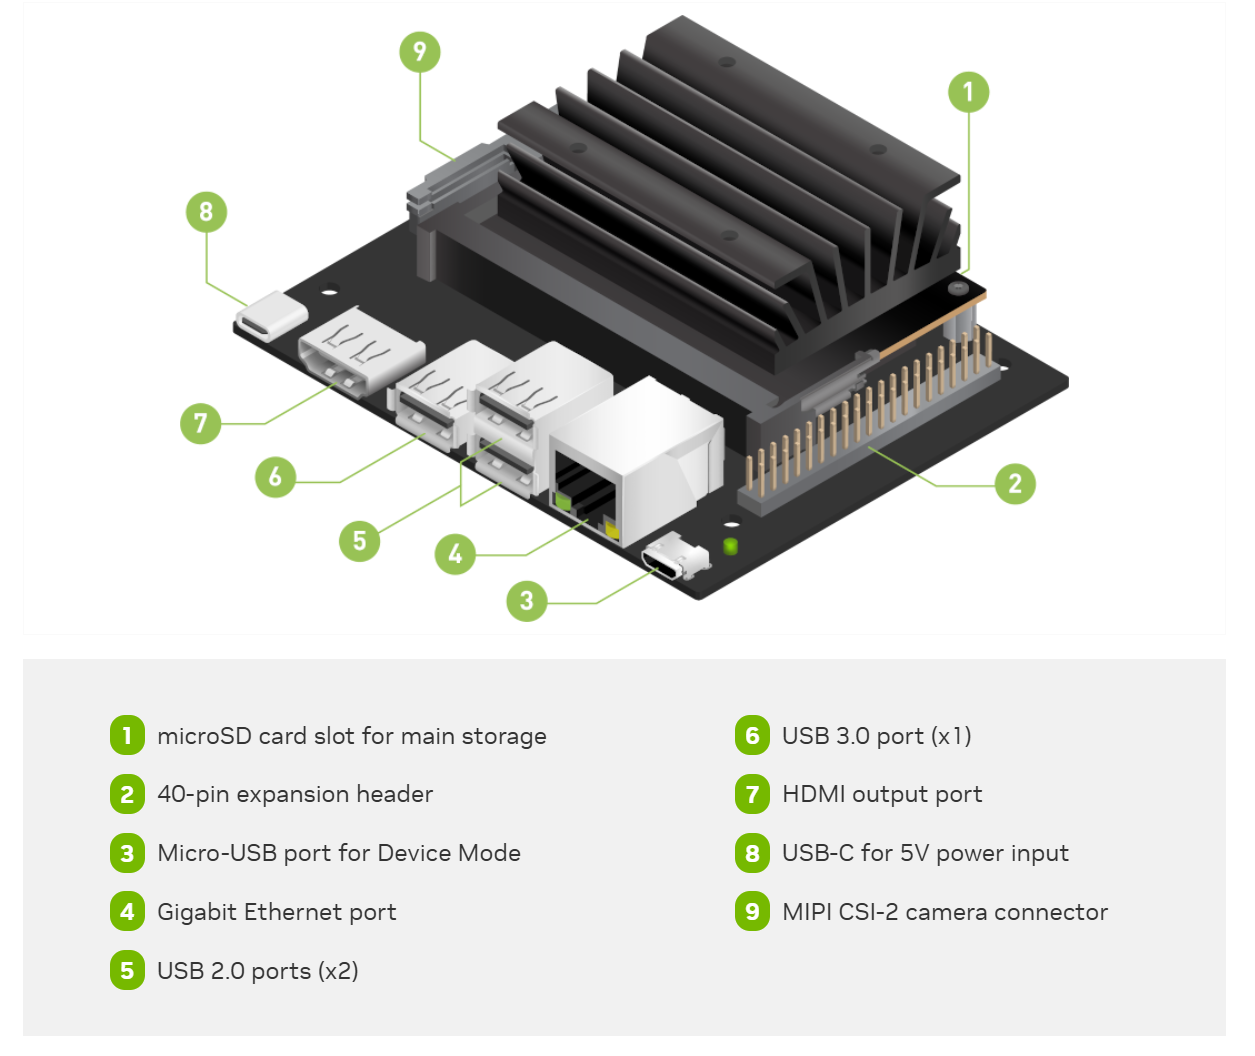
\includegraphics[width=0.4\linewidth]{images/Jetson1.png}
    \caption{NVIDIA Jetson Nano 2GB Developer Kit connectivity.}
    \label{fig:jetson_connectivity}
\end{figure}

The board operates within a typical power envelope of 5W to 10W, making it suitable for energy-constrained embedded and edge-computing scenarios. \\
The platform supports the NVIDIA JetPack SDK, which includes optimized libraries such as CUDA, cuDNN, and TensorRT for hardware-accelerated deep learning inference \cite{nvidia_corporation_jetson_nodate}.
\\
The presence of a dedicated GPU enables on-device execution of convolutional neural networks for tasks such as object detection and image segmentation, reducing latency compared to cloud-based solutions and enabling near real-time inference in edge environments. 

Despite its limited memory capacity (2GB LPDDR4) and constrained power budget, the Maxwell GPU architecture allows the Jetson Nano to achieve competitive inference performance for several state-of-the-art deep learning models. To quantitatively assess its computational capabilities, representative inference benchmarks are reported in Table~\ref{tab:jetson_benchmarks} \cite{moe_long_nvidia_nodate}. The values are expressed in frames per second (FPS) under optimized inference configurations.

\begin{table}[h]
\centering
\begin{tabular}{l c}
\hline
\textbf{Model} & \textbf{Performance (FPS)} \\
\hline
Inception-v4 & 10.51 \\
VGG-19 & 9.95 \\
Super-resolution (BSD500) & 15.12 \\
U-Net (segmentation) & 16.57 \\
Pose estimation & 14.47 \\
YOLOv3-Tiny (416$\times$416) & 47.11 \\
ResNet-50 (224$\times$224) & 36.42 \\
SSD MobileNet-v1 & 42.00 \\
\hline
\end{tabular}
\caption{Representative inference performance of NVIDIA Jetson Nano 2GB.}
\label{tab:jetson_benchmarks}
\end{table}

As shown in Table~\ref{tab:jetson_benchmarks} \cite{moe_long_nvidia_nodate}, lightweight architectures such as YOLOv3-Tiny and SSD MobileNet-v1 achieve real-time performance, while more computationally demanding networks (e.g., VGG-19 and Inception-v4) operate at lower frame rates. These results highlight the importance of selecting architectures that balance accuracy and computational complexity when deploying deep learning models on resource-constrained embedded platforms.
\\
It should be noted that the reported performance values may vary depending on the software configuration, precision mode (e.g., FP16 or INT8), and system workload.


Considering the trade-off between computational performance, power consumption, cost, and ecosystem support, the Jetson Nano 2GB represents a suitable platform for prototyping and deploying computer vision algorithms in embedded systems, as in the present application.
\clearpage
\subsection{Azure Microsoft Kinect DK}
% !TeX root = ../../tesi.tex

For the acquisition of RGB-D data at Site~1, the \textbf{Microsoft Azure Kinect DK} \cite{microsoft_azure_nodate} was employed. This device is a spatial sensing platform developed by Microsoft, designed for advanced computer vision, depth sensing, and AI-based perception applications.

\begin{figure}[h]
    \centering
    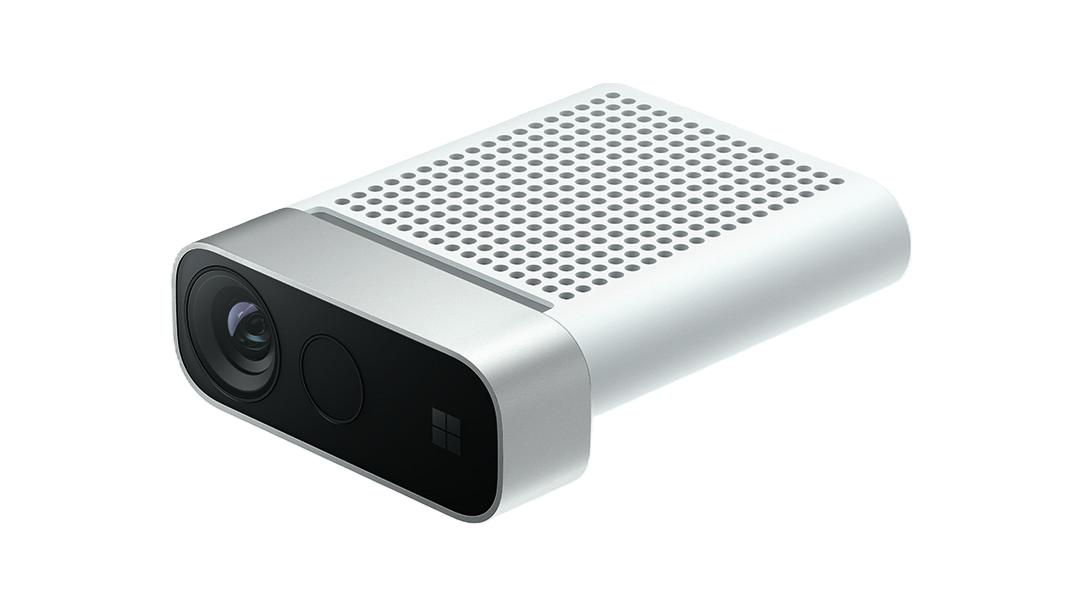
\includegraphics[width=0.6\linewidth]{images/azure-kinect.jpg}
    \caption{Microsoft Azure Kinect DK}
    \label{fig:azure-kinect}
\end{figure}

The Azure Kinect DK integrates a high-resolution RGB camera and a depth sensor based on Time-of-Flight (ToF) technology. The RGB camera provides up to 12~MP resolution (4096$\times$3072), while the depth sensor delivers depth maps with a maximum resolution of 1024$\times$1024 pixels.

The depth sensing module operates using modulated infrared light to estimate per-pixel distance information, enabling accurate 3D scene reconstruction \cite{microsoft_about_nodate}.

The device supports multiple depth operating modes, including Narrow Field of View (NFOV) and Wide Field of View (WFOV), each configurable with binned and unbinned resolutions, as illustrated in Figure~\ref{fig:camera-fov} and in Table~\ref{tab:azure_depth_modes}. This flexibility allows adaptation to different working distances and spatial accuracy requirements. The depth measurement range typically varies between 0.25~m and 5.5~m, depending on the selected configuration and environmental conditions \cite{microsoft_about_nodate}.

\begin{figure}[h]
    \centering
    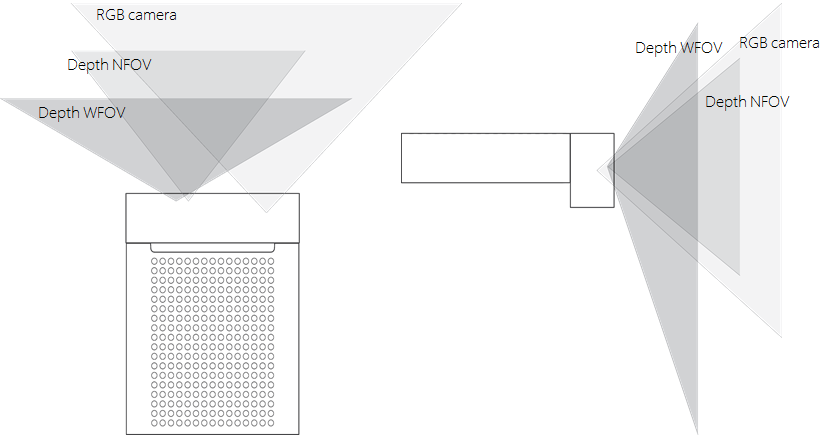
\includegraphics[width=0.70\linewidth]{images/camera-fov.png}
    \caption{Available depth sensor fields of view (NFOV and WFOV).}
    \label{fig:camera-fov}
\end{figure}

\newpage
Depending on the selected RGB resolution and depth operating mode, the camera parameters, field of view, frame rate, and operational range vary significantly. \\The main RGB camera configurations are reported in Table~\ref{tab:azure_rgb_modes}, while the available depth modes are summarized in Table~\ref{tab:azure_depth_modes}.

\begin{table}[h]
    \centering
    \renewcommand{\arraystretch}{1.2}
    \resizebox{\textwidth}{!}{
    \begin{tabular}{|l|c|l|c|c|}
        \hline
        \textbf{RGB Resolution (HxV)} & \textbf{Aspect Ratio} & \textbf{Format} & \textbf{FPS} & \textbf{Nominal FoV (HxV)} \\
        \hline
        3840$\times$2160 & 16:9 & MJPEG & 0, 5, 15, 30 & 90$^\circ$$\times$59$^\circ$ \\
        2560$\times$1440 & 16:9 & MJPEG & 0, 5, 15, 30 & 90$^\circ$$\times$59$^\circ$ \\
        1920$\times$1080 & 16:9 & MJPEG & 0, 5, 15, 30 & 90$^\circ$$\times$59$^\circ$ \\
        1280$\times$720  & 16:9 & MJPEG / YUY2 / NV12 & 0, 5, 15, 30 & 90$^\circ$$\times$59$^\circ$ \\
        4096$\times$3072 & 4:3  & MJPEG & 0, 5, 15 & 90$^\circ$$\times$74.3$^\circ$ \\
        2048$\times$1536 & 4:3  & MJPEG & 0, 5, 15, 30 & 90$^\circ$$\times$74.3$^\circ$ \\
        \hline
    \end{tabular}
    }
    \caption{RGB camera operating modes and specifications.}
    \label{tab:azure_rgb_modes}
\end{table}

\begin{table}[h]
    \centering
    \small
    \renewcommand{\arraystretch}{1.2}
    \begin{tabular}{|l|c|c|c|c|c|}
        \hline
        \textbf{Mode} & \textbf{Resolution} & \textbf{FoV} & \textbf{FPS} & \textbf{Operating Range} & \textbf{Exposure Time} \\
        \hline
        NFOV unbinned & 640$\times$576 & 75$\times$65$^\circ$ & 0, 5, 15, 30 & 0.5 -- 3.86 m & 12.8 ms \\
        NFOV 2$\times$2 binned & 320$\times$288 & 75$\times$65$^\circ$ & 0, 5, 15, 30 & 0.5 -- 5.46 m & 12.8 ms \\
        WFOV 2$\times$2 binned & 512$\times$512 & 120$\times$120$^\circ$ & 0, 5, 15, 30 & 0.25 -- 2.88 m & 12.8 ms \\
        WFOV unbinned & 1024$\times$1024 & 120$\times$120$^\circ$ & 0, 5, 15 & 0.25 -- 2.21 m & 20.3 ms \\
        Passive IR & 1024$\times$1024 & N/A & 0, 5, 15, 30 & N/A & 1.6 ms \\
        \hline
    \end{tabular}
    \caption{Depth camera operating modes and specifications.}
\label{tab:azure_depth_modes}
\end{table}
From a hardware standpoint, the Azure Kinect DK includes:
\begin{itemize}
    \item one 12~MP RGB camera,
    \item one Time-of-Flight depth sensor,
    \item one 6-axis inertial measurement unit (IMU),
    \item one USB-C interface for power and data transmission,
    \item one external synchronization port for multi-device configurations.
\end{itemize}

\begin{figure}[h]
    \centering
    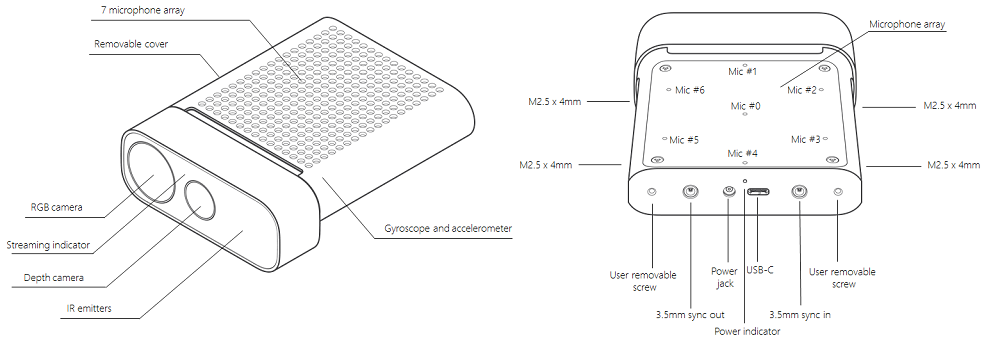
\includegraphics[width=0.8\linewidth]{images/kinect.png}
    \caption{Microsoft Azure Kinect DK hardware and connectivity.}
    \label{fig:kinect}
\end{figure}

The availability of synchronized RGB and depth streams enables the generation of geometrically aligned RGB-D frames, which are particularly suitable for 3D reconstruction, volumetric estimation, and point cloud generation. In the present application, depth information is exploited to estimate the volume of dough samples by reconstructing their three-dimensional point-cloud.

\subsubsection{Time-of-Flight Depth Sensing Principle}
% !TeX root = ../../tesi.tex

The depth sensing module of the Microsoft Azure Kinect DK is based on the Time-of-Flight (ToF) principle, a technique used to estimate the distance between the sensor and objects in the scene by measuring the time required for emitted light to travel to the target and back to the sensor.
\begin{figure}[h]
    \centering
    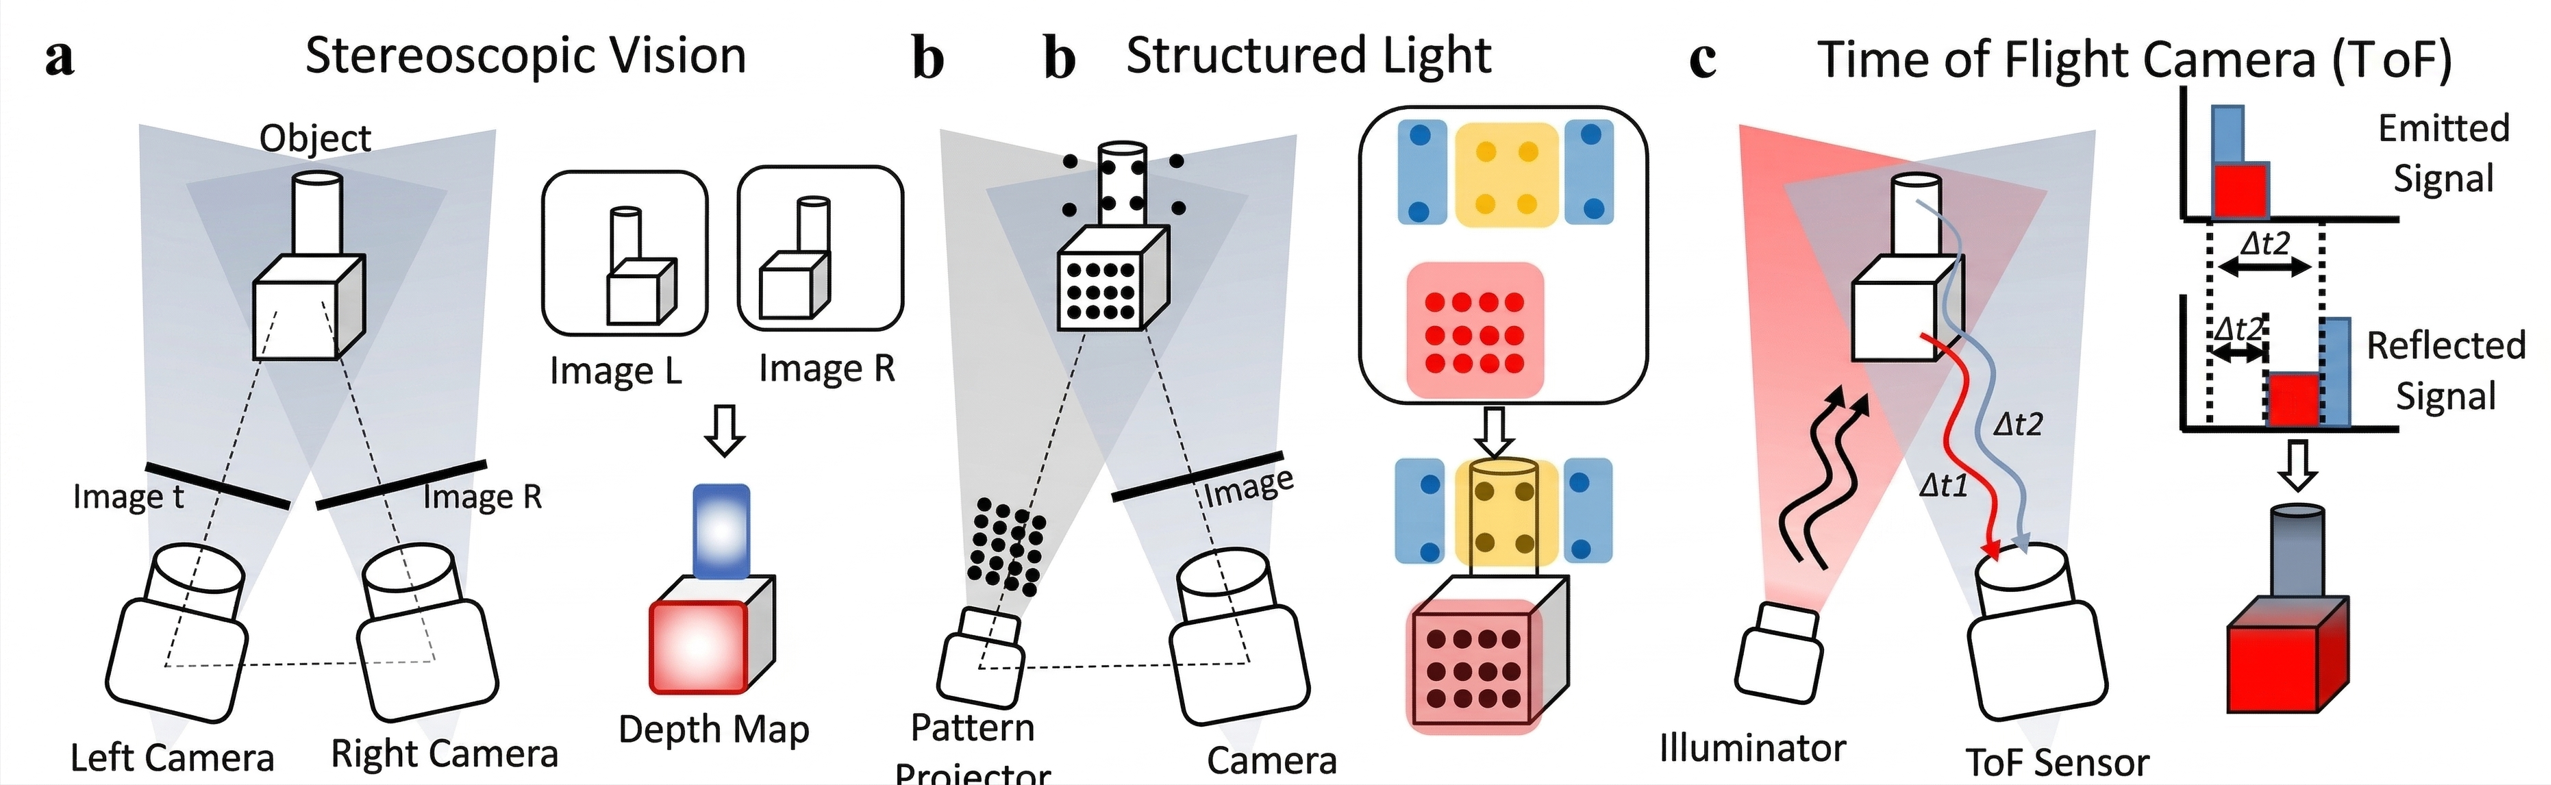
\includegraphics[width=0.7\linewidth]{images/ToF.png}
    \caption{Different depth estimation approaches}
    \label{fig:Depth}
\end{figure}

In general, the depth $Z$ of a point can be computed as:

\begin{equation}
Z = \frac{c \cdot \Delta t}{2}
\end{equation}

where:
\begin{itemize}
    \item $c$ is the speed of light in air,
    \item $\Delta t$ is the round-trip travel time of the emitted optical signal.
    \item The division by two accounts for the two-way propagation path (sensor-to-object and object-to-sensor).
\end{itemize}

Direct measurement of $\Delta t$ requires extremely high temporal resolution, as light travels approximately 30~cm in 1~ns. For this reason, most modern ToF cameras, including the Azure Kinect, employ a \textit{continuous-wave modulation} approach rather than direct pulsed time measurement.

\begin{figure}[h]
    \centering
    \includegraphics[width=0.5\linewidth]{images/ToF_pulse_vs_cont.jpg}
    \caption{Different ToF approaches}
    \label{fig:ToF_1}
\end{figure}

In continuous-wave ToF systems, the emitted infrared light is amplitude-modulated at a known frequency. The reflected signal received by the sensor exhibits a phase shift $\phi$ proportional to the propagation delay. The depth is then computed as:

\begin{equation}
Z = \frac{c}{4\pi f} \phi
\end{equation}

where:
\begin{itemize}
    \item $f$ is the modulation frequency,
    \item $\phi$ is the measured phase difference between emitted and received signals.
\end{itemize}

\begin{figure}[h]
    \centering
    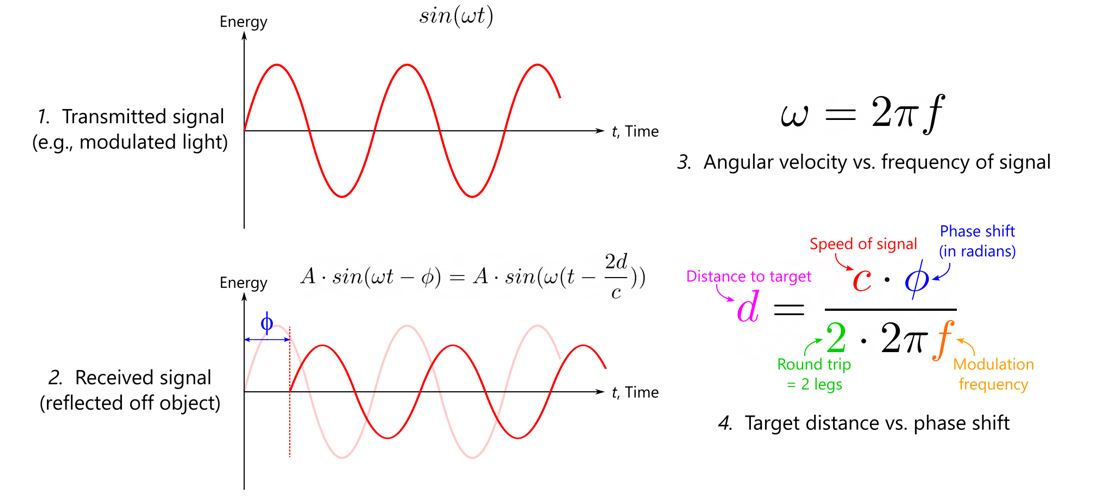
\includegraphics[width=0.7\linewidth]{images/ToF_1.jpg}
    \caption{Time of flight equations derivation}
    \label{fig:ToF_2}
\end{figure}

By estimating the phase shift at each pixel, the sensor generates a dense depth map, enabling per-pixel 3D reconstruction of the observed scene.
\\
The advantages of ToF-based depth sensing include:
\begin{itemize}
    \item direct acquisition of metric depth measurements,
    \item dense depth maps without requiring stereo matching,
    \item robustness to moderate textureless surfaces.
\end{itemize}

However, ToF systems are subject to several sources of error, including:
\begin{itemize}
    \item multipath interference (MPI), caused by indirect reflections,
    \item ambient infrared light interference,
    \item phase ambiguity at larger distances due to periodic modulation,
    \item reduced accuracy on highly reflective or absorptive materials.
\end{itemize}

Despite these limitations, Time-of-Flight technology provides accurate and dense depth measurements in indoor environments, making it particularly suitable for volumetric estimation and 3D reconstruction tasks, as required in the present application.


\subsubsection{Azure Kinect Sensor SDK}

The Azure Kinect DK is supported by the Azure Kinect Sensor SDK \cite{microsoft_azure-kinect-sensor-sdk_2026}, which provides low-level APIs for device control, stream acquisition, intrinsic and extrinsic calibration handling, depth-to-color transformation, and point cloud extraction \cite{microsoft_about_nodate}.

The SDK exposes calibrated camera parameters, including focal lengths, principal points, and distortion coefficients, enabling accurate geometric transformations between RGB and depth coordinate systems. Moreover, built-in functions allow real-time depth image rectification, coordinate mapping, and conversion of depth frames into 3D point clouds expressed in camera reference coordinates.

Such capabilities are particularly relevant in volumetric estimation tasks, where precise spatial alignment between depth measurements and RGB data is required to ensure geometrical consistency.
\begin{figure}[h]
    \centering
    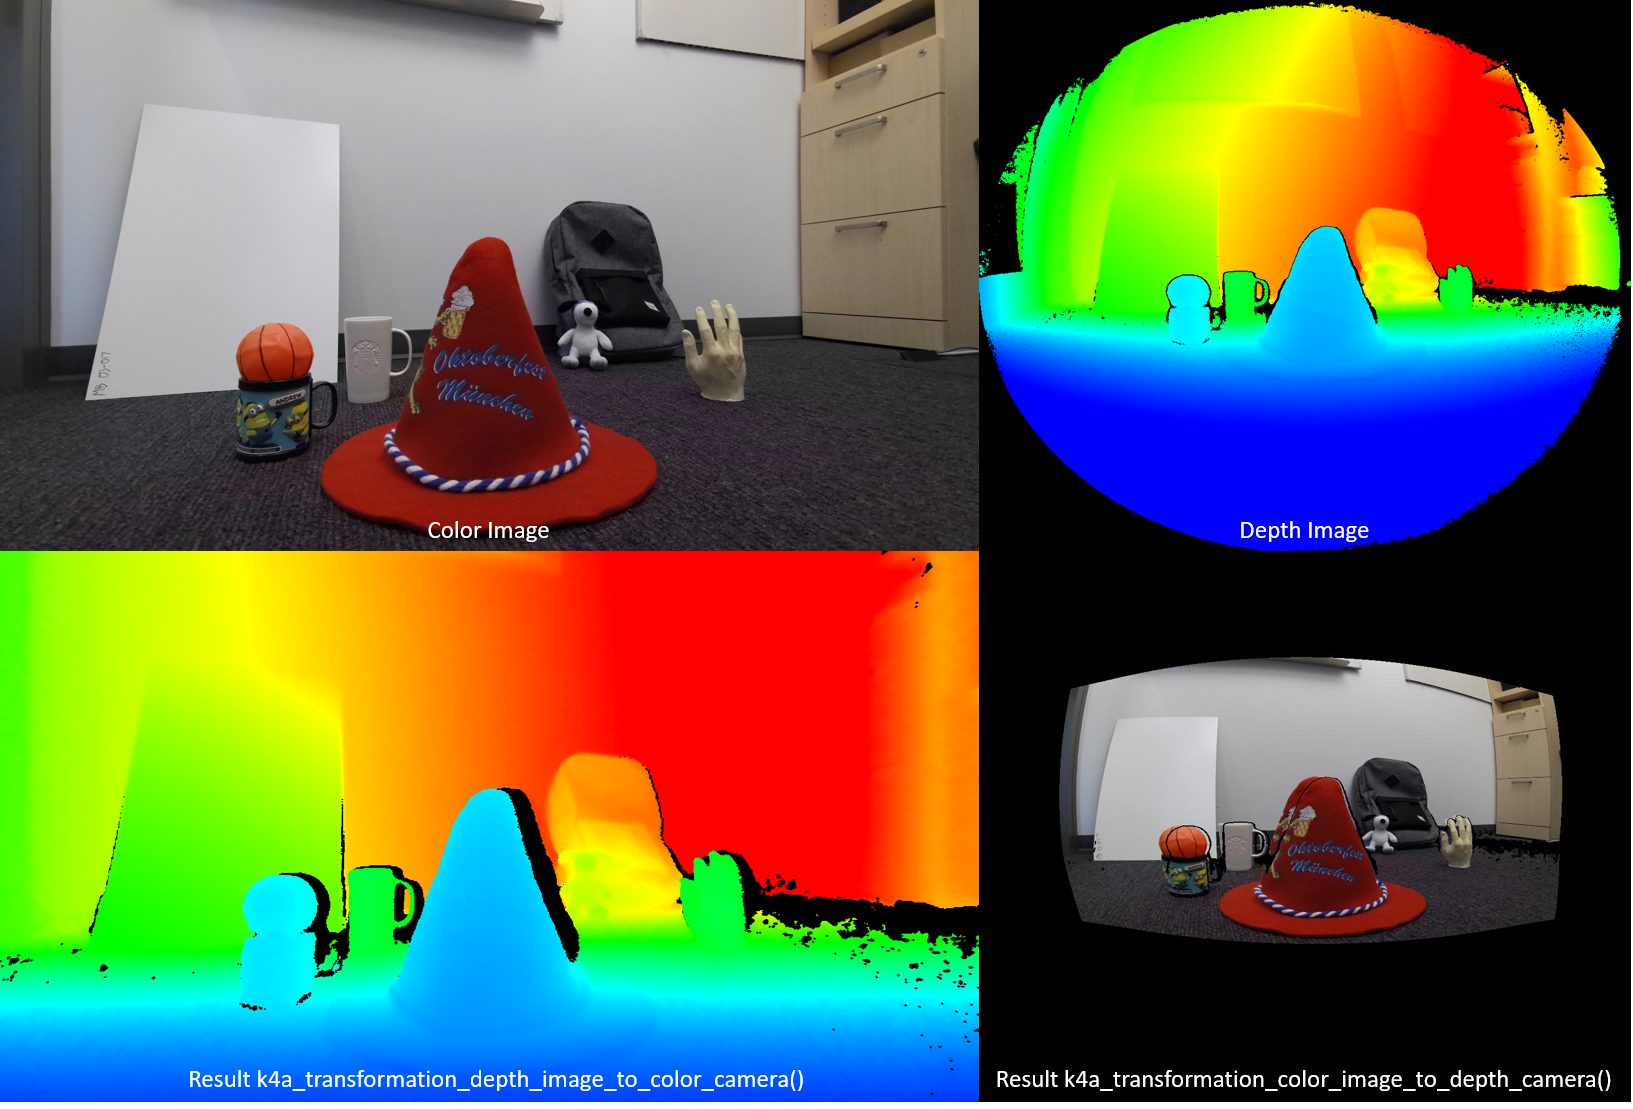
\includegraphics[width=0.5\linewidth]{images/sdk.png}
    \caption{Example of SDK transformation from depth image to color camera FOV and viceversa}
    \label{fig:SDK}
\end{figure}

\subsubsection{Python Wrapper: pyKinectAzure}
For integration within the data processing pipeline, a Python interface was adopted through the \textit{pyKinectAzure} wrapper \cite{gorordo_fernandez_pykinectazure_2026}. This open-source library provides Python bindings to the native Azure Kinect Sensor SDK, allowing device initialization, stream acquisition, frame synchronization, and calibration access directly from Python environments.

The wrapper enables rapid prototyping and seamless integration with scientific computing libraries such as NumPy and OpenCV. Through pyKinectAzure, depth frames can be converted into NumPy arrays, facilitating further processing steps such as filtering, segmentation, and 3D point cloud generation within the same software ecosystem used for machine learning and computer vision tasks.

The use of a Python wrapper significantly simplifies the development workflow while maintaining access to the underlying calibrated sensor data and geometric transformation utilities provided by the official SDK.

Considering its depth accuracy, configurable field of view, synchronized RGB-D acquisition capabilities, and extensive software support, the Microsoft Azure Kinect DK represents a suitable sensing solution for industrial computer vision applications requiring reliable volumetric measurements.

\section{Site 2: Baked Bread Dataset Acquisition and Color Analysis}
% !TeX root = ../../tesi.tex

Site 2 corresponds to the acquisition and inspection station dedicated to baked bread loaves. In contrast to Site 1, where RGB-D data are exploited to estimate volumetric properties of raw dough balls, Site 2 focuses on the visual analysis of the final baked product. The primary objective at this stage is the creation of a dedicated image dataset of baked loaves, followed by the training and deployment of the DEIMv2 object detection network for automated detection and anomaly-based quality assessment.

\subsection{Industrial Context and Monitoring Objectives}

At Site 2, the product has completed the baking process and is transported along the production line as finished bread loaves. At this stage, geometric variability is less critical than the overall visual appearance of the final product, including crust condition, browning patterns, and other surface irregularities. These characteristics may reflect deviations in baking quality and in the underlying process parameters.\\
The system deployed at Site 2 aims to:

\begin{itemize}
    \item Acquire a representative dataset of baked bread images,
    \item Train a dedicated DEIMv2 object detection model,
    \item Detect bread loaves in real time,
    \item Support anomaly-based quality monitoring of the final product.
\end{itemize}

\begin{figure}[h]
    \centering
    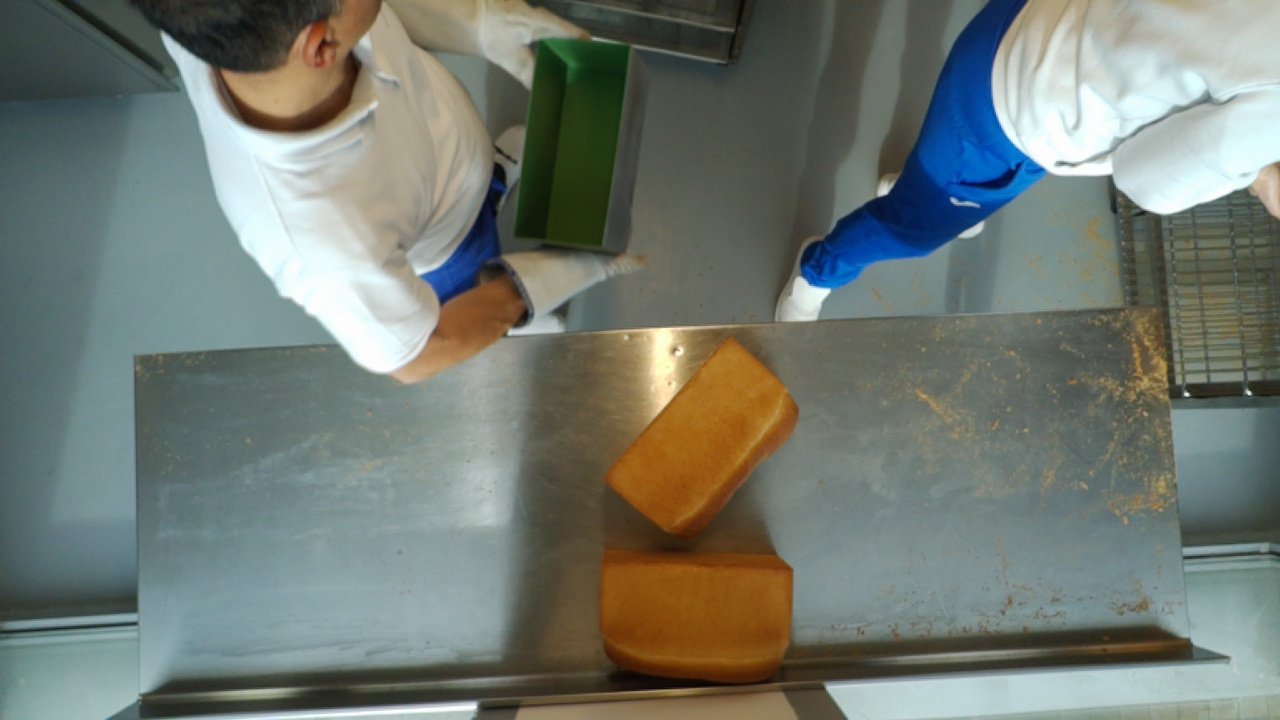
\includegraphics[width=0.65\linewidth]{images/Site2_breadloaf.jpg}
    \caption{Point of view of the Raspberry Pi Camera Module 3 Wide during the manual extraction phase, showing operators removing baked bread loaves from the trays under real production conditions}
    \label{fig:breadloaf}
\end{figure}

\subsection{Dataset Creation}

During the initial phase, the system operates in data acquisition mode. Following the same motion-triggered acquisition principle adopted at Site~1, images of baked bread loaves are captured by using background subtraction as an event trigger. At this site, the assessment is not based on depth cues but on visual characteristics such as color, illumination, and surface texture. For this reason, images are acquired under controlled lighting conditions to reduce visual variability due to the environment (see \emph{Practical challenges and system robustness} in Chapter~1) and to improve the consistency of both the collected dataset and the resulting analysis.

The collected dataset is subsequently annotated through an automatic labelling strategy based on Lang-SAM \cite{medeiros_luca-medeiroslang-segment-anything_2026} and used to train the DEIMv2 \cite{huang_real-time_2026} object detection network in an offline environment with higher computational resources. The details of the automatic labelling strategy and training procedure are described in Chapter~4.

This dataset creation phase is fundamental to ensure robustness of the detection model against variations in loaf shape, surface texture, illumination changes, and partial occlusions.

\subsection{Hardware Configuration}

Unlike Site 1, which relies on an RGB-D sensor and embedded GPU platform, Site 2 adopts a lightweight and cost-effective vision setup composed of:

\begin{itemize}
    \item A Raspberry Pi 5 \cite{raspberrypi_raspberry_pi_5_2026} for edge computation,
    \item A Raspberry Pi Camera Module 3 Wide \cite{raspberrypi_camera_documentation_2026} for RGB image acquisition.
\end{itemize}

The Raspberry Pi Camera Module 3 Wide provides a large field of view, enabling coverage of the table where the loaves are baked (as shown in Figure~\ref{fig:breadloaf}). Since volumetric estimation is not required at this stage, depth sensing is unnecessary, and a monocular RGB configuration is sufficient.

\subsection{Online Detection and Downstream Analysis}

Once training is completed, the DEIMv2 model is deployed on the Raspberry Pi 5 \cite{raspberrypi_raspberry_pi_5_2026} for inference. For each acquired RGB frame, the bread loaves are detected and the corresponding image regions are extracted. These regions are then passed to a downstream anomaly-detection stage for product-quality assessment. The detailed pipeline and anomaly-detection procedure are presented in Chapter~4.

\subsection{Role of Site 2 in the Overall Architecture}

Site 2 complements the functionality of Site 1 by extending the inspection framework from geometric analysis of raw dough to anomaly-based visual assessment of the final baked product. While Site 1 leverages RGB-D sensing for volumetric estimation, Site 2 employs a monocular RGB setup for anomaly detection on baked bread loaves.

Together, the two sites demonstrate the flexibility of the proposed DEIM-based architecture, which can be adapted to different sensing modalities and quality metrics while maintaining a consistent edge-computing paradigm.

\subsection{Raspberry Pi 5}
% !TeX root = ../../tesi.tex

For the computations at Site~2, namely RGB image acquisition, local control of the sensing pipeline, and execution of lightweight edge-processing tasks, the \textbf{Raspberry Pi 5} was adopted.\cite{raspberrypi_raspberry_pi_5_2026} In contrast to Site~1, where an RGB-D sensor and an embedded GPU platform were required for volumetric estimation, Site~2 relies on a monocular RGB setup and therefore benefits from a more compact and cost-effective embedded computer.

\begin{figure}[h]
    \centering
    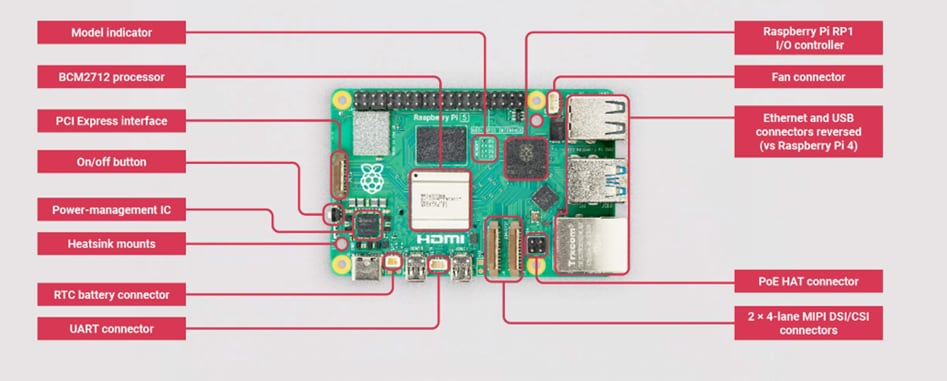
\includegraphics[width=0.7\textwidth]{images/Raspberry.jpg}
    \caption{Raspberry Pi 5 board.}
    \label{fig:rpi5_board}
\end{figure}

The Raspberry Pi 5 is a single-board computer developed for embedded and edge-computing applications.\cite{raspberrypi_raspberry_pi_5_2026} It is based on the Broadcom BCM2712 system-on-chip, which integrates a \textbf{quad-core Arm Cortex-A76 CPU running at 2.4~GHz}, a \textbf{VideoCore~VII GPU}, and \textbf{8~GB of LPDDR4X memory} in the configuration adopted for this project.\cite{raspberrypi_raspberry_pi_5_2026}

From a hardware standpoint, the Raspberry Pi 5 provides a wide set of interfaces that are particularly relevant for computer-vision deployments, including:
\begin{itemize}
    \item two USB~3.0 ports and two USB~2.0 ports,
    \item Gigabit Ethernet,
    \item dual-band Wi-Fi and Bluetooth connectivity,
    \item two four-lane MIPI transceivers for camera and display interfaces,
    \item a PCIe~2.0 interface for high-speed peripheral expansion,
    \item a USB-C power input.\cite{raspberrypi_raspberry_pi_5_2026}
\end{itemize}

These characteristics make the platform flexible enough to support local image acquisition, communication with external devices, and integration with dedicated sensing peripherals such as the Raspberry Pi Camera Module~3 Wide discussed in the following subsection.\cite{raspberrypi_raspberry_pi_hardware_2026}

An important practical aspect of the Raspberry Pi 5 is that its increased computing performance, compared with earlier Raspberry Pi boards, is accompanied by a higher thermal load under sustained workloads. Since the device in the present application is expected to operate continuously for long periods, potentially day and night and without constant supervision, it is important to equip it with an active cooling system in order to reduce the risk of thermal throttling and to maintain stable performance under prolonged load.\cite{raspberrypi_raspberry_pi_5_2026} For this reason, the board was installed inside a protective case equipped with a fan, as shown in Figure~\ref{fig:rpi5_site2}.

\begin{figure}[h]
    \centering
    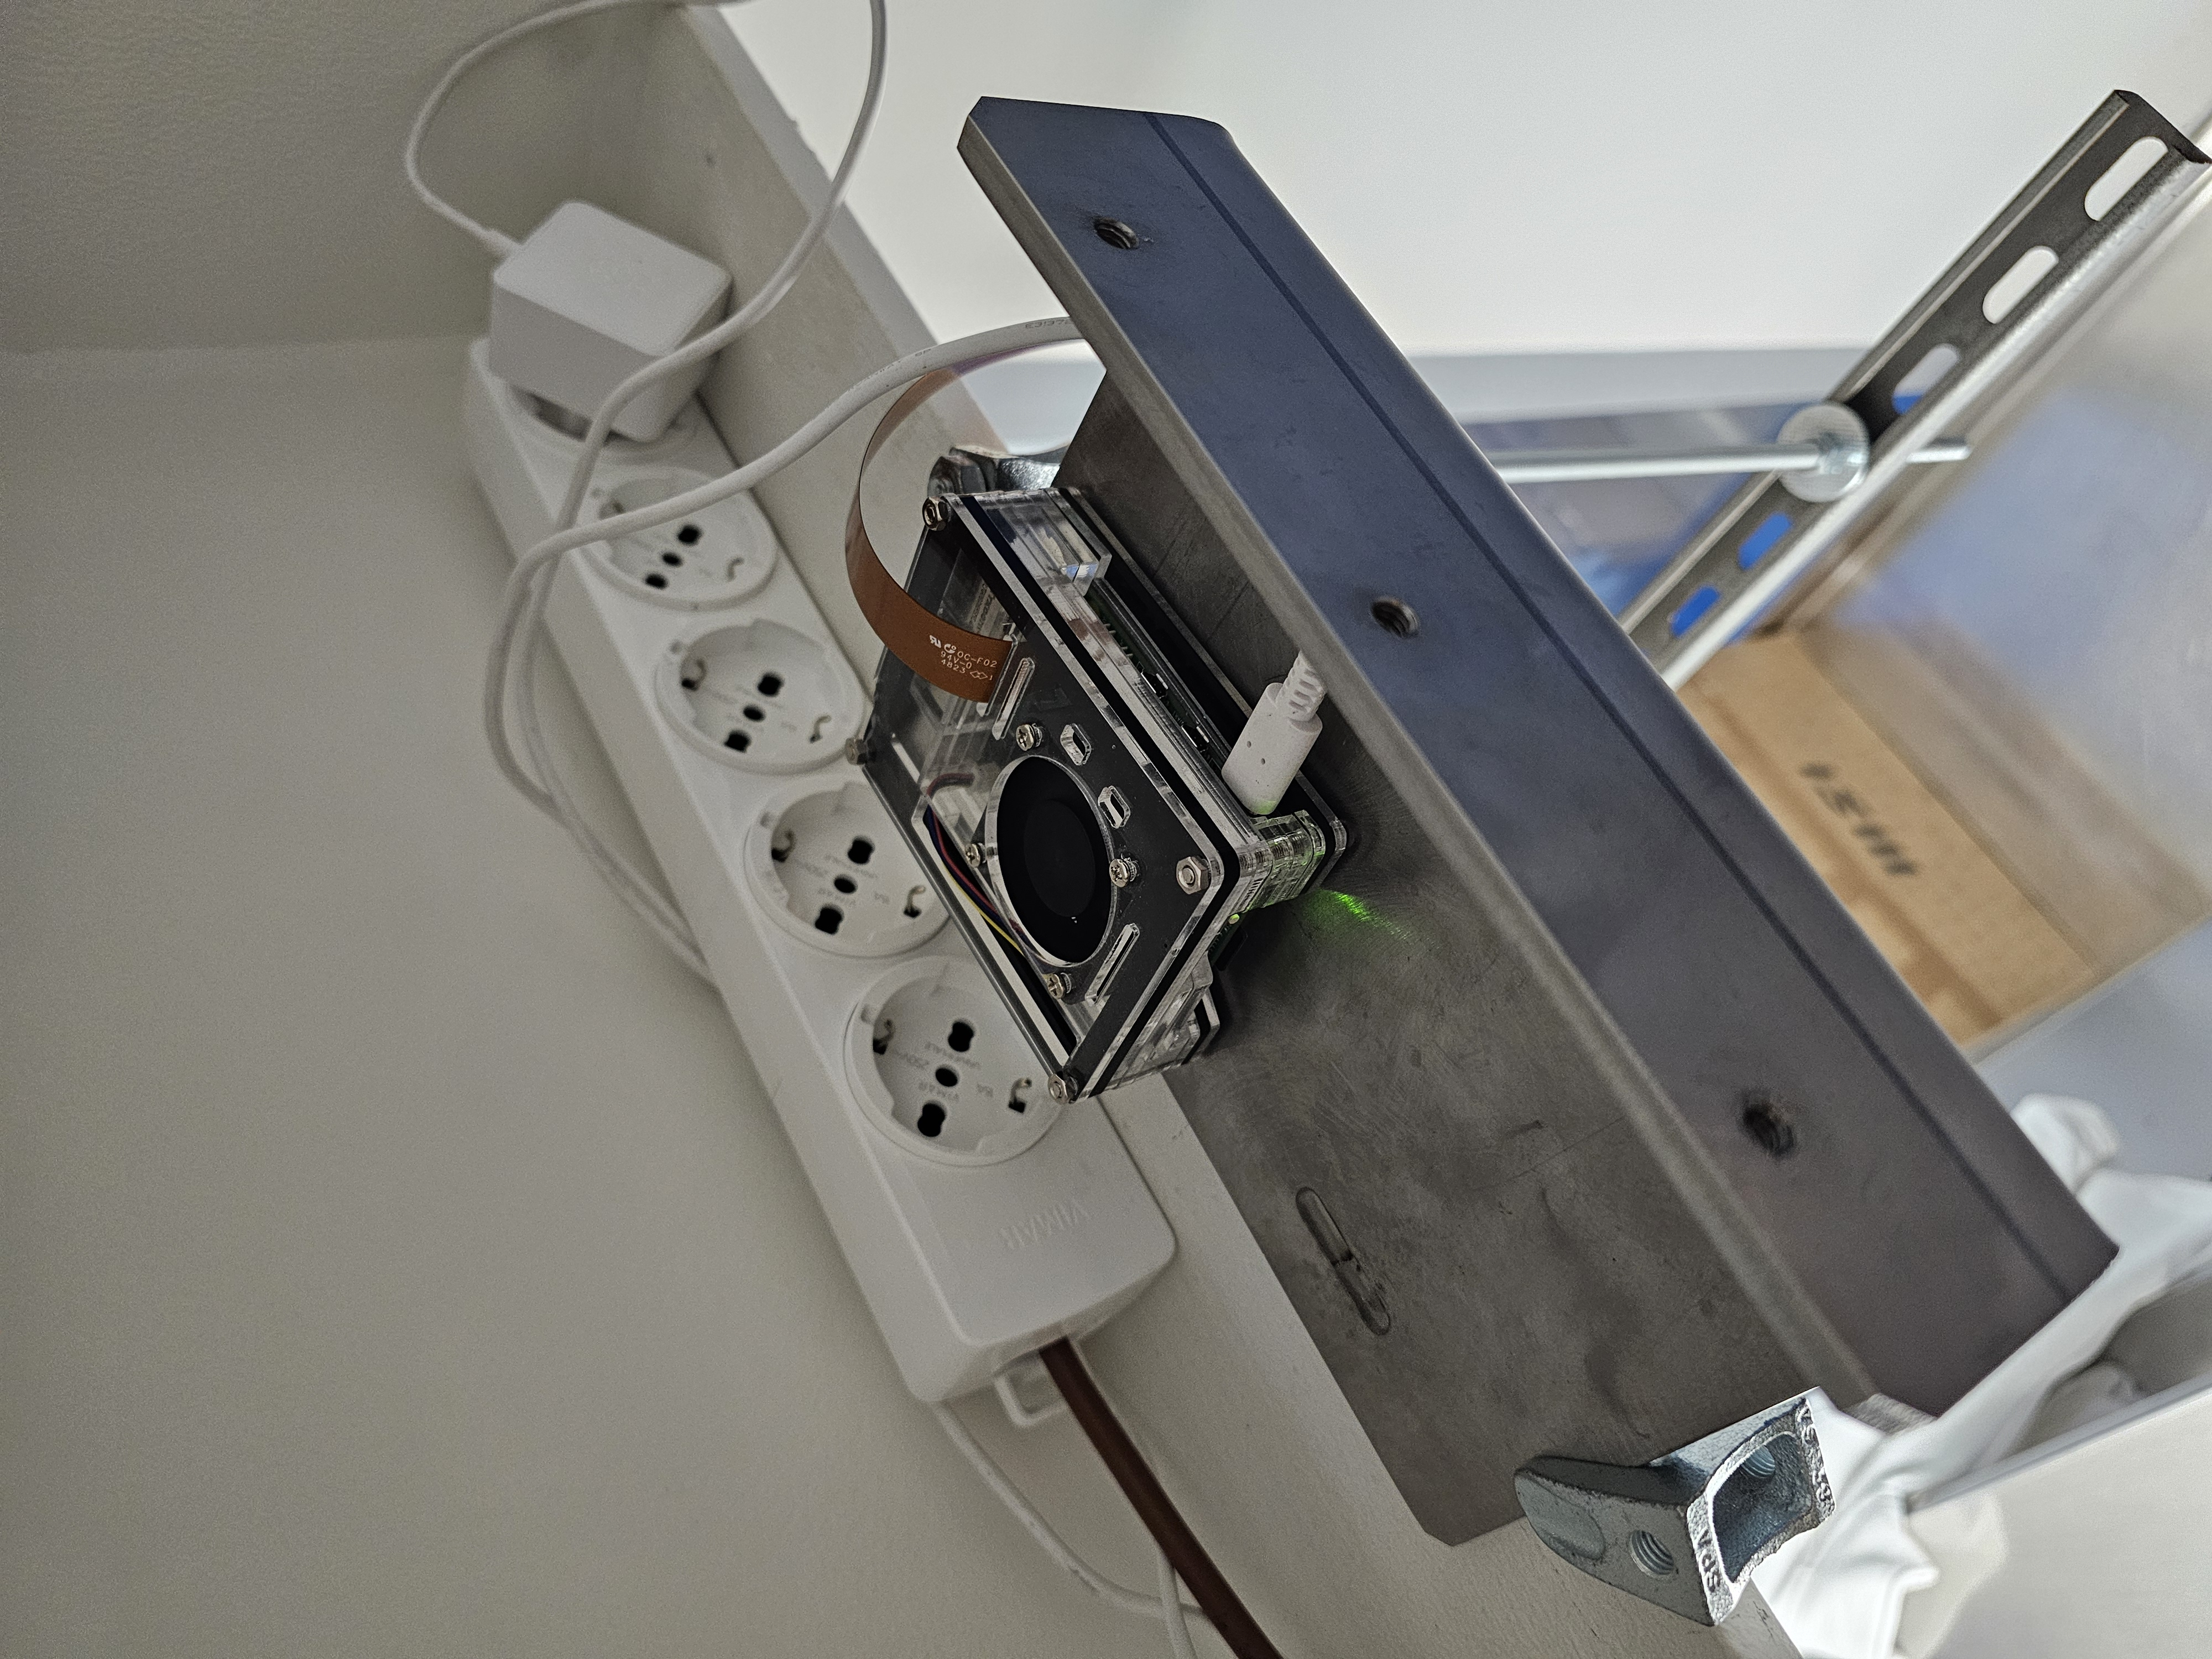
\includegraphics[width=0.6\textwidth, angle=-90]{images/Raspberry_sito2.jpg}
    \caption{Raspberry Pi 5 installed on Site~2 inside a protective case with active cooling.}
    \label{fig:rpi5_site2}
\end{figure}

From the perspective of the present application, the Raspberry Pi 5 offers several advantages: compact size, low power requirements, straightforward integration with official Raspberry Pi peripherals, and sufficient computational capability for a lightweight vision pipeline at the edge. At the same time, compared with more specialized embedded AI platforms such as the Jetson Nano, it provides a less dedicated acceleration stack for deep-learning inference. In this sense, its adoption at Site~2 is justified by the lower sensing complexity of the setup, which is based only on RGB imagery and does not require real-time RGB-D reconstruction or point-cloud processing. Considering the trade-off between computational capability, ease of integration, cost, and deployment simplicity, the Raspberry Pi 5 represents a suitable hardware platform for Site~2.\cite{raspberrypi_raspberry_pi_5_2026,raspberrypi_raspberry_pi_hardware_2026}

\subsection{Raspberry Pi Camera Module 3 Wide}
% !TeX root = ../../tesi.tex

For RGB acquisition at Site~2, the \textbf{Raspberry Pi Camera Module~3 Wide} was employed.\cite{raspberrypi_camera_module_3_2026} This device is an official Raspberry Pi imaging sensor designed for embedded vision applications and directly interfaced to the Raspberry Pi 5 through the CSI camera interface.

\begin{figure}[h]
    \centering
    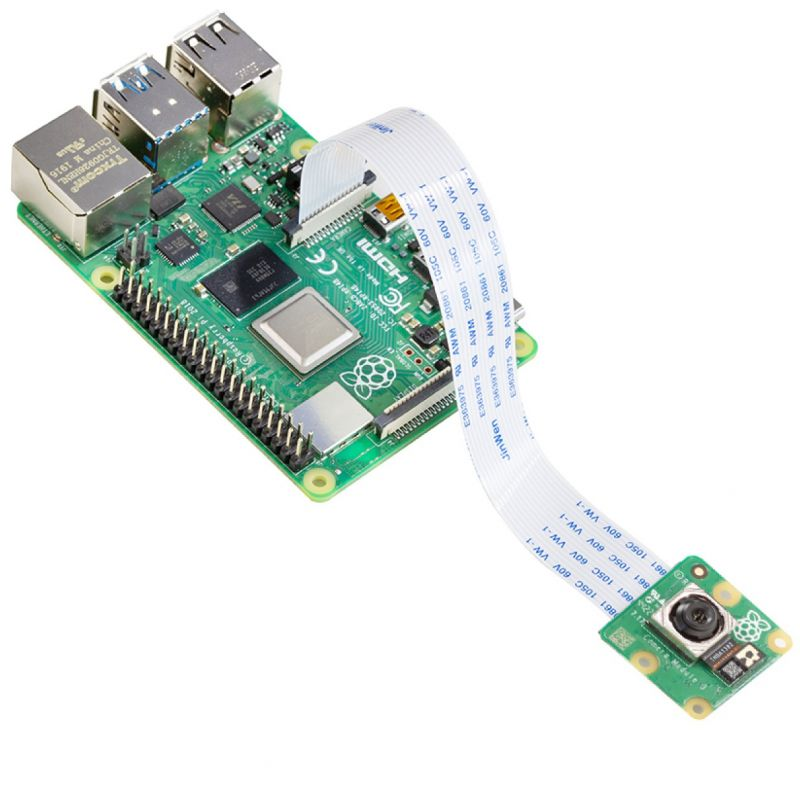
\includegraphics[width=0.3\textwidth]{images/Raspberry-Pi-Camera-Module-3-Wide.jpg}
    \caption{Raspberry Pi Camera Module~3 Wide mounted on a Raspberry Pi 5 board.}
    \label{fig:rpi_camera3_wide_board}
\end{figure}

The Camera Module~3 family is built around the \textbf{Sony IMX708} image sensor, which provides a resolution of approximately \textbf{11.9~MP} (4608$\times$2592 pixels).\cite{raspberrypi_camera_module_3_2026} In addition to its relatively high spatial resolution, the module supports \textbf{autofocus} through phase-detection autofocus and includes \textbf{HDR} capabilities, making it suitable for embedded vision tasks in which scene conditions may vary over time.\cite{raspberrypi_camera_module_3_2026,raspberrypi_camera_documentation_2026}

The \textbf{Wide} variant was selected because it provides a \textbf{120$^\circ$ diagonal field of view}, which is particularly useful in industrial environments where the camera must cover a relatively broad working area from a short mounting distance.\cite{raspberrypi_camera_module_3_2026} In the present setup, this characteristic is important because the system must observe the table area in which baked loaves are manually removed from the trays, which is relatively large and located at a distance of approximately 1.5~m from the camera.

\begin{figure}[h]
    \centering
    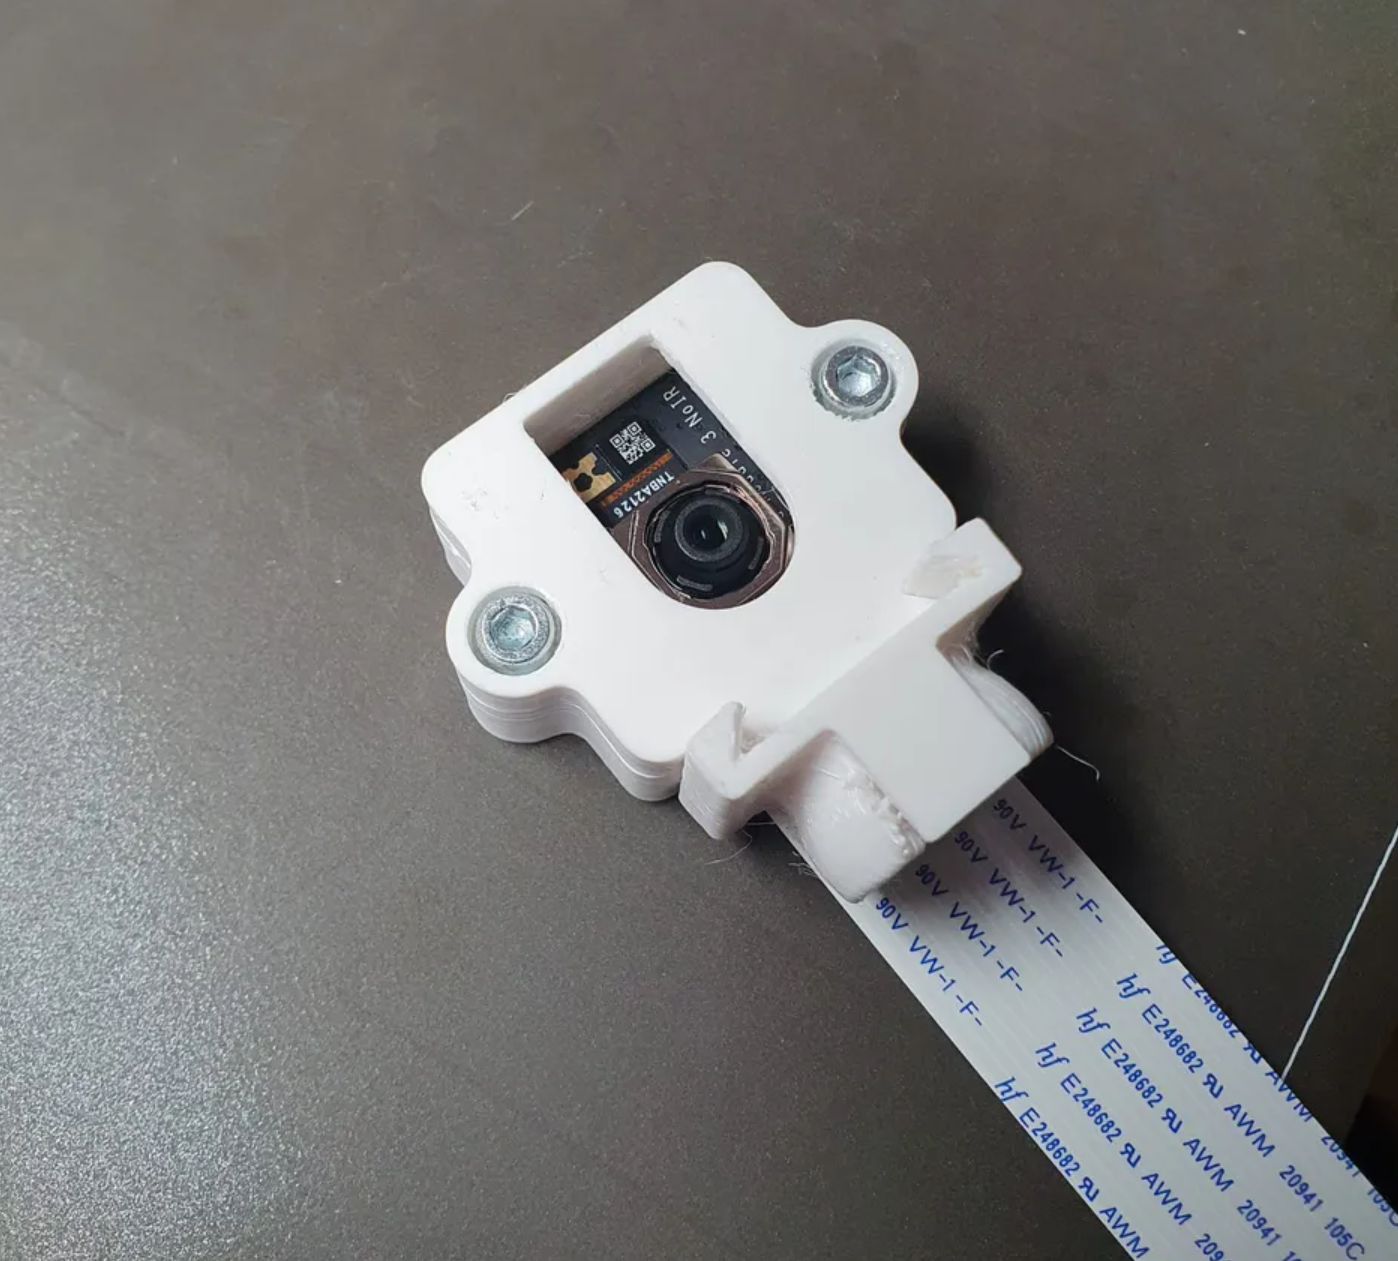
\includegraphics[width=0.4\textwidth]{images/Raspicam_3D-model.png}
    \caption{3D model of the Raspberry Pi Camera Module~3 Wide.}
    \label{fig:rpi_camera3_wide_model}
\end{figure}

To improve the practical integration of the camera into the Site~2 workstation, a dedicated housing solution was developed by starting from an existing online case model and modifying it for the specific constraints of the installation. The resulting enclosure was then fabricated through 3D printing. This solution was engineered to fit the geometry of the available station and to support a stable and repeatable mounting configuration for data acquisition. Besides providing mechanical protection, it improved cable management and helped maintain a more consistent camera placement under the specific operating conditions of the industrial environment, as shown in Figure~\ref{fig:rpi_camera3_wide_site2}.

\begin{figure}[h]
    \centering
    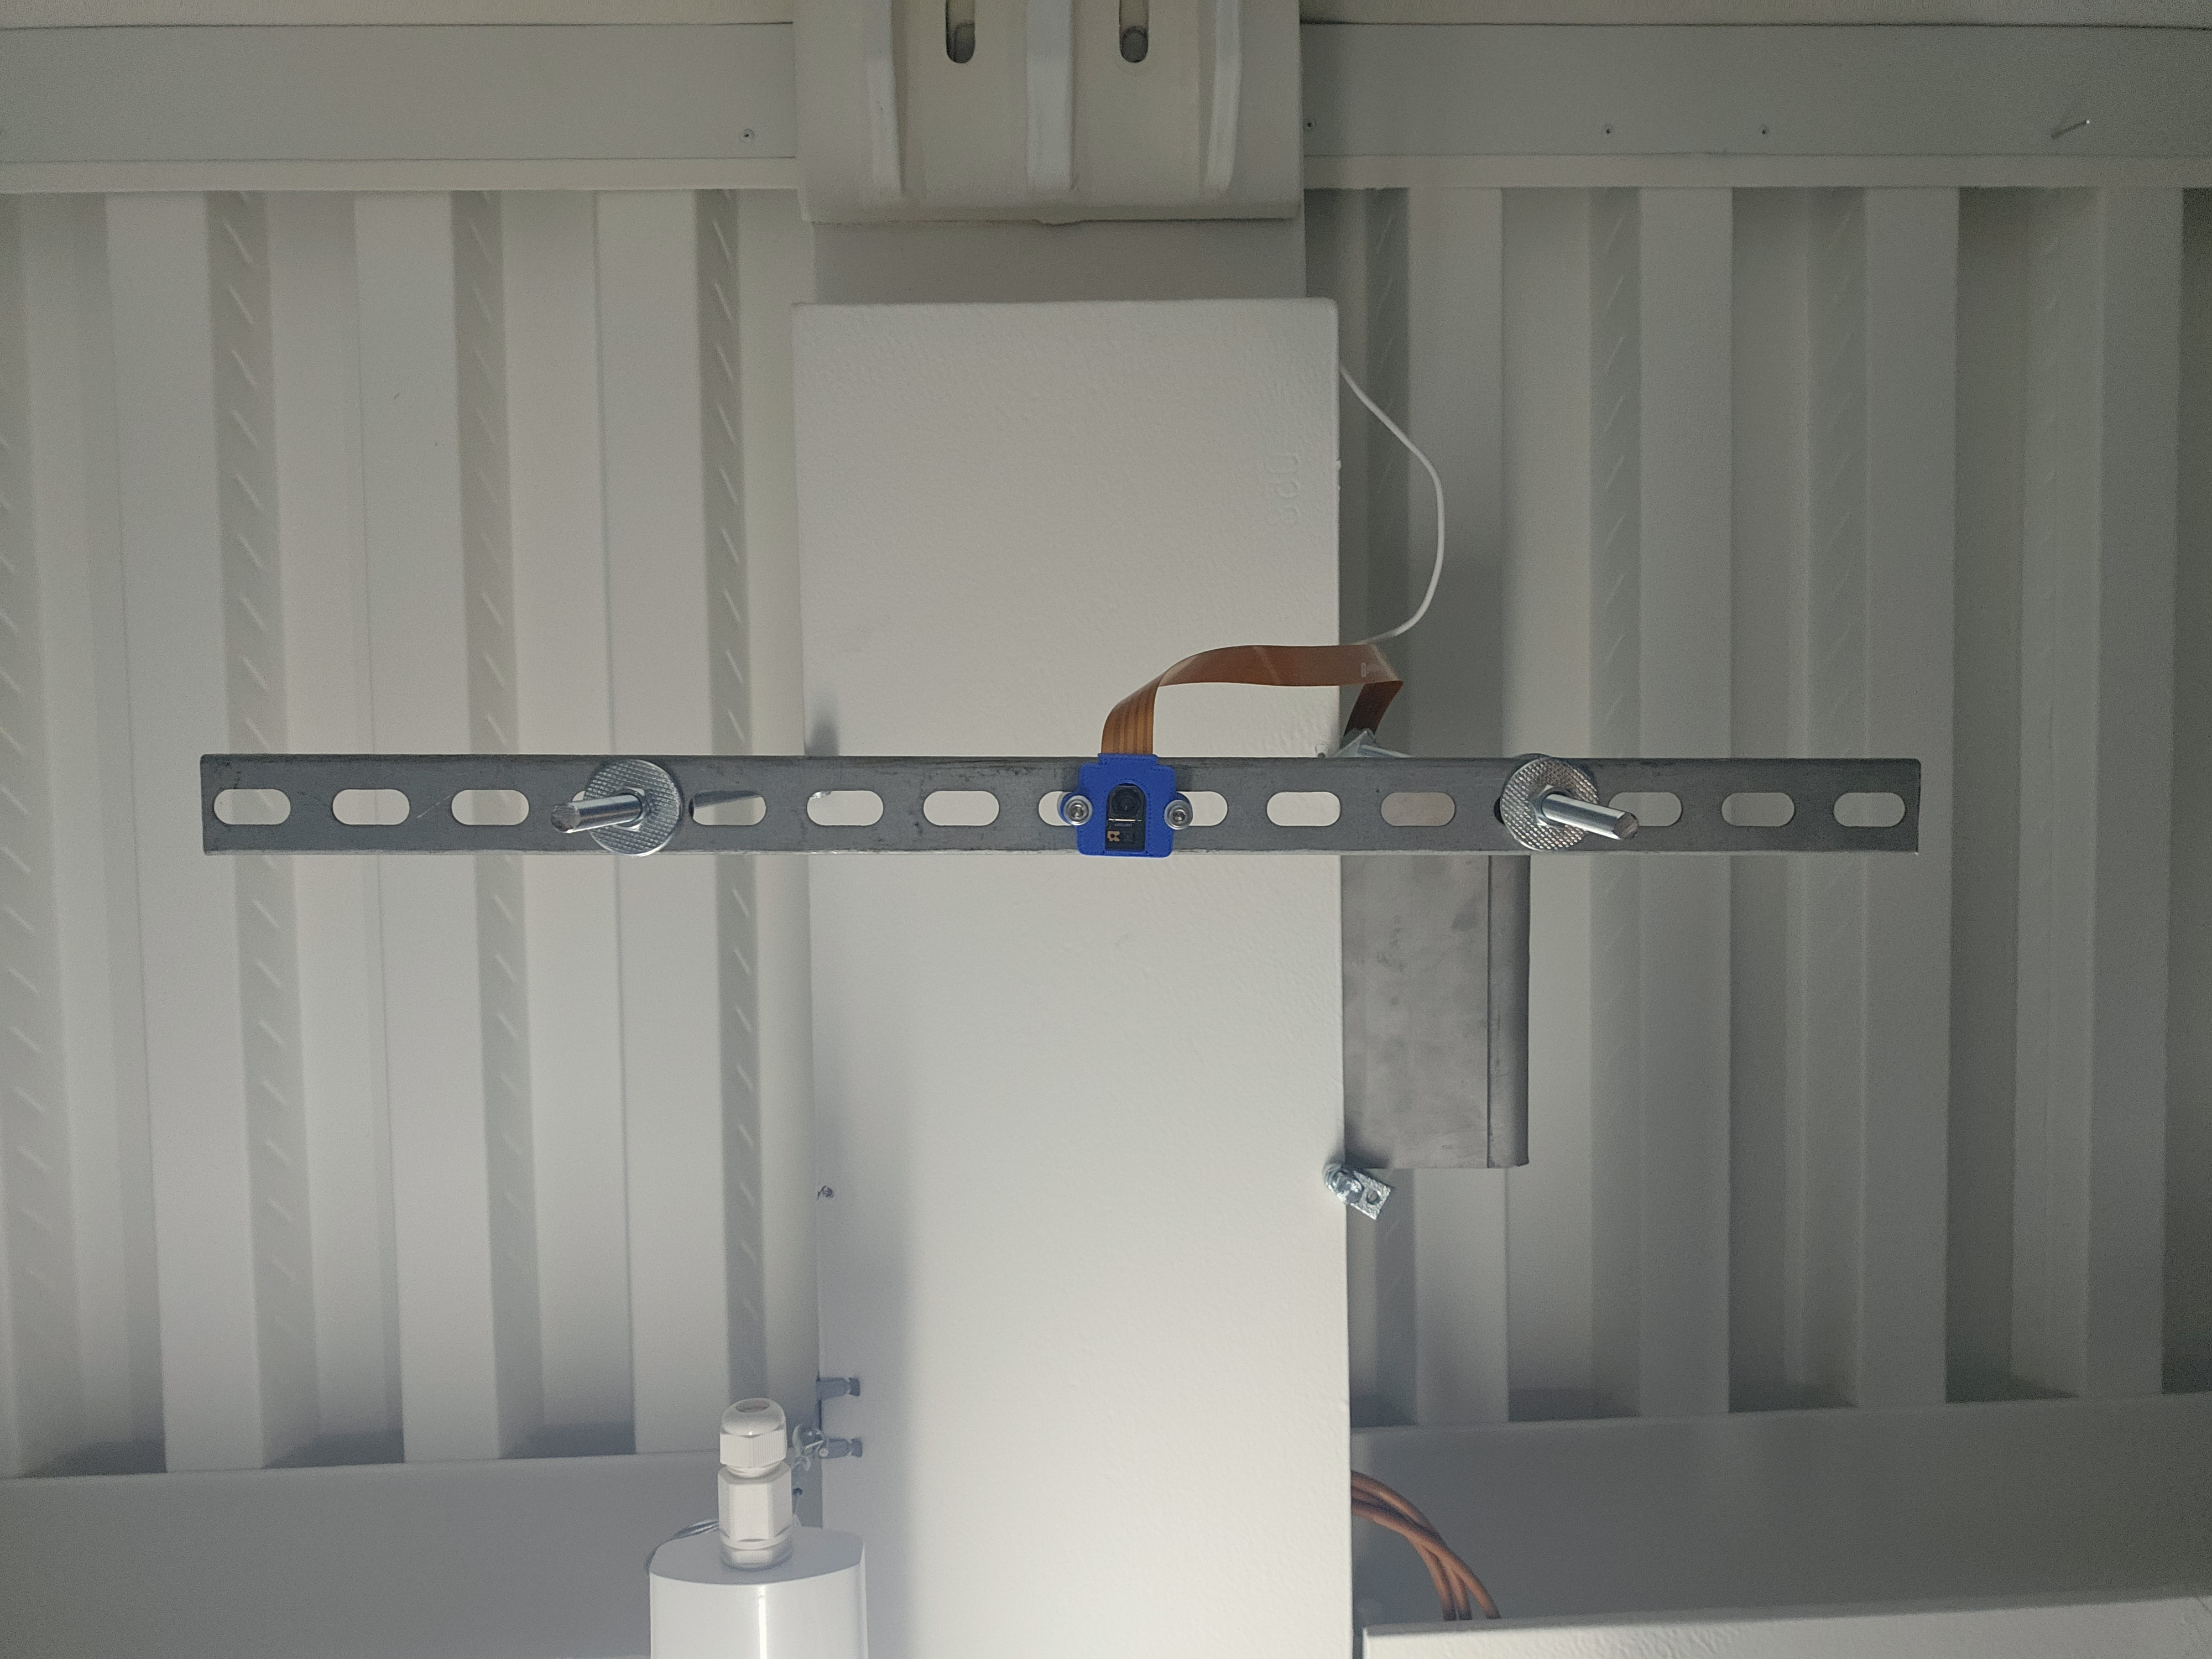
\includegraphics[width=0.5\textwidth, angle=90]{images/Raspberry_site2.jpg}
    \caption{Custom 3D-printed case for the Raspberry Pi Camera Module~3 Wide, placed in the Site~2 workstation.}
    \label{fig:rpi_camera3_wide_site2}
\end{figure}
\newpage
From an operational point of view, the camera module supports still-image acquisition at full sensor resolution and multiple video modes suitable for embedded computer-vision pipelines, including Full HD video and higher-frame-rate lower-resolution modes.\cite{raspberrypi_camera_module_3_2026,raspberrypi_camera_documentation_2026} The native integration with the Raspberry Pi ecosystem also simplifies software development through the official camera stack based on \textit{libcamera} and \textit{Picamera2}.\cite{raspberrypi_camera_documentation_2026}

For the purposes of this thesis, the Camera Module~3 Wide offers several practical advantages, including a field of view well suited to the inspection area, autofocus capability, and tight hardware and software integration with the Raspberry Pi 5. At the same time, the use of a monocular RGB camera also introduces some limitations. Unlike the Azure Kinect employed at Site~1, the Raspberry Pi Camera Module~3 Wide does not provide depth information and therefore cannot support direct 3D reconstruction. Moreover, because the sensing modality is purely RGB-based, the quality of the acquired data remains sensitive to lighting conditions, shadows, and viewpoint-dependent appearance changes. For this reason, illumination control and camera placement remain important aspects of the Site~2 setup, as illustrated in Figure~\ref{fig:faretto_sito2}. Overall, the Raspberry Pi Camera Module~3 Wide represents a suitable sensing solution for Site~2 thanks to its wide field of view, autofocus capability, compact form factor, and seamless compatibility with the Raspberry Pi platform.\cite{raspberrypi_camera_module_3_2026,raspberrypi_camera_documentation_2026}

\subsubsection{Picamera2 Library}
% !TeX root = ../../tesi.tex

For the integration of the Raspberry Pi Camera Module~3 Wide within the acquisition pipeline, the \textit{Picamera2} library was adopted.\cite{raspberrypi_picamera2_manual_2026,raspberrypi_picamera2_github_2026} Picamera2 is the Python interface built on top of the Raspberry Pi \textit{libcamera} stack and represents the modern replacement for the legacy Picamera interface.\cite{raspberrypi_picamera2_github_2026}

The library provides high-level access to camera initialization, stream configuration, frame acquisition, metadata handling, and camera controls such as exposure, gain, and autofocus.\cite{raspberrypi_picamera2_manual_2026} These features are particularly useful in embedded computer-vision applications, where the camera must be configured programmatically and integrated into a broader software pipeline.

In the present project, Picamera2 enabled direct access to RGB frames from Python, thereby simplifying the interaction between the camera and the processing software based on NumPy and OpenCV. This made it possible to implement image acquisition, parameter tuning, and frame extraction within the same software environment used for the rest of the pipeline.

Compared with lower-level camera handling, Picamera2 provides a practical abstraction that accelerates development while still exposing the controls needed for embedded deployment. This was particularly useful not only for the implementation of the acquisition pipeline itself, but also for the two-week automated data-collection phase, in which a stable and well-supported software interface was essential to manage continuous image acquisition and reliable data storage over extended periods. For this reason, Picamera2 represented a suitable software interface for Site~2, where ease of integration, reliability, and compatibility with the Raspberry Pi ecosystem were important design requirements.\cite{raspberrypi_picamera2_manual_2026,raspberrypi_picamera2_github_2026}


\subsection{PiCamera}
% !TeX root = ../../tesi.tex

For the integration of the Raspberry Pi Camera Module~3 Wide within the acquisition pipeline, the \textit{Picamera2} library was adopted.\cite{raspberrypi_picamera2_manual_2026,raspberrypi_picamera2_github_2026} Picamera2 is the Python interface built on top of the Raspberry Pi \textit{libcamera} stack and represents the modern replacement for the legacy Picamera interface.\cite{raspberrypi_picamera2_github_2026}

The library provides high-level access to camera initialization, stream configuration, frame acquisition, metadata handling, and camera controls such as exposure, gain, and autofocus.\cite{raspberrypi_picamera2_manual_2026} These features are particularly useful in embedded computer-vision applications, where the camera must be configured programmatically and integrated into a broader software pipeline.

In the present project, Picamera2 enabled direct access to RGB frames from Python, thereby simplifying the interaction between the camera and the processing software based on NumPy and OpenCV. This made it possible to implement image acquisition, parameter tuning, and frame extraction within the same software environment used for the rest of the pipeline.

Compared with lower-level camera handling, Picamera2 provides a practical abstraction that accelerates development while still exposing the controls needed for embedded deployment. This was particularly useful not only for the implementation of the acquisition pipeline itself, but also for the two-week automated data-collection phase, in which a stable and well-supported software interface was essential to manage continuous image acquisition and reliable data storage over extended periods. For this reason, Picamera2 represented a suitable software interface for Site~2, where ease of integration, reliability, and compatibility with the Raspberry Pi ecosystem were important design requirements.\cite{raspberrypi_picamera2_manual_2026,raspberrypi_picamera2_github_2026}

 %File in cui è scritto il capitolo
\label{chapter:chapter_4} %Label per creare riferimenti al capitolo
% !TeX root = ../../tesi.tex

\chapter{Multimodal quality inspection framework}

\section{Pipeline}
% !TeX root = ../../tesi.tex

The implemented framework follows a shared offline--online logic across the two industrial sites, while adapting the final processing stage to the different monitoring objectives of raw dough and baked bread. In both cases, the first phase consists of autonomous image acquisition on an embedded edge device. The collected data are then transferred to an offline workstation, automatically labelled, and used to train a DEIMv2 detector. Once training is completed, the detector is redeployed on the edge hardware and becomes the entry point of the online inspection pipeline.\cite{labby_thesis_repo_2026,labby_kinect_acquisition_2026} The overall architecture was designed in a \textbf{modular} way, so that different detection, reconstruction, and downstream-analysis modules could be tested, replaced, or extended without rewriting the entire workflow.\cite{labby_thesis_repo_2026}

At \textbf{Site~1}, the acquisition stage relies on synchronized RGB-D frames from the Azure Kinect.\cite{microsoft_azure_nodate} After online detection, each dough ball is associated with aligned depth information and converted into a local 3D representation for volumetric analysis. The adopted workflow includes an initial color-clustering stage, subsequent foreground segmentation and refinement with respect to the reference table model, 3D completion of the observed geometry, and volume estimation through multiple geometric methods.\cite{labby_thesis_repo_2026}

At \textbf{Site~2}, the acquisition stage is based on RGB images from the Raspberry Pi Camera Module~3 Wide.\cite{raspberrypi_camera_module_3_2026} After online detection, the localized bread loaves are cropped and forwarded to an anomaly-detection stage implemented with EfficientAD through anomalib.\cite{batzner_efficientad_2024,akcay_anomalib_2022} In this case, the detector acts as a region proposal mechanism, while the downstream anomaly model estimates how strongly each loaf deviates from the normal appearance learned from production data.\cite{labby_thesis_repo_2026}


\section{Motion Detection}
% !TeX root = ../../tesi.tex

\subsubsection{Background Subtraction for Motion Triggering}
During the data-acquisition phase, images are not recorded continuously. Instead, the acquisition framework monitors the scene through a configurable background-subtraction stage and stores a frame only when motion is detected inside the selected region of interest (ROI).\cite{opencv_background_subtraction_2026,labby_kinect_acquisition_2026}
\\
In this way, the saved dataset is concentrated around the actual passage of dough balls or bread loaves, while long intervals of static background are discarded.
\begin{figure}[h]
    \centering
    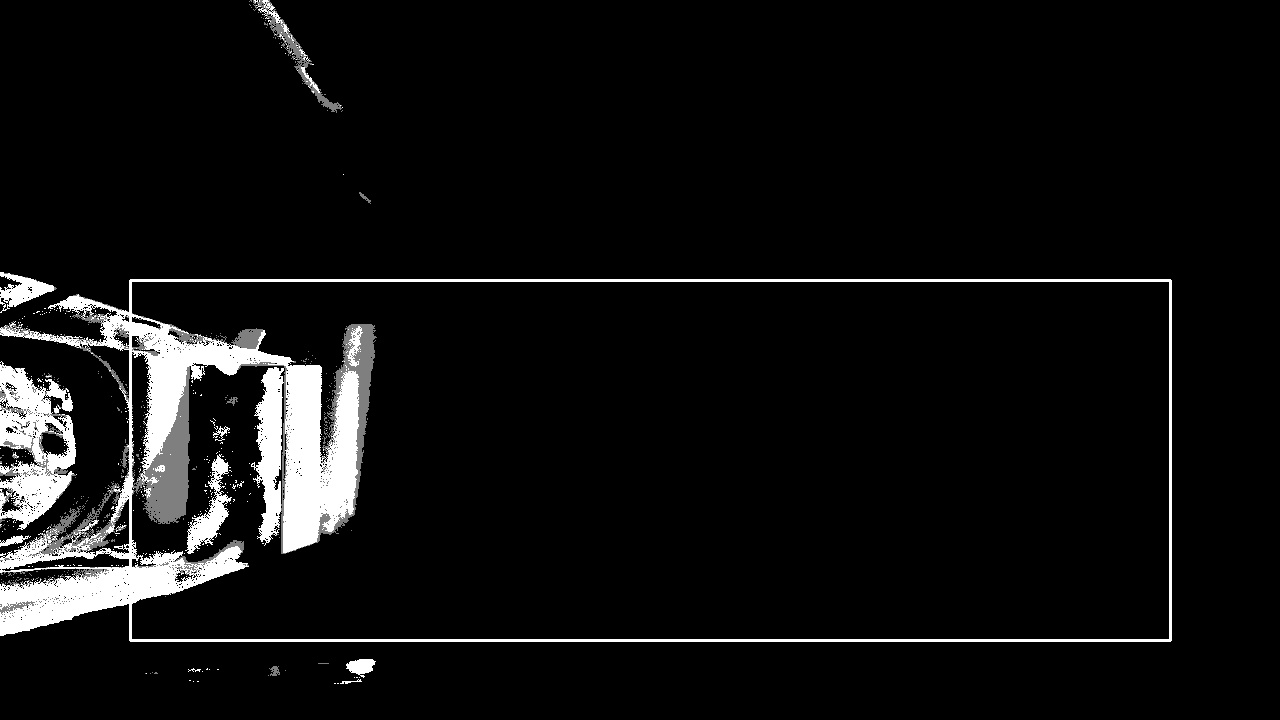
\includegraphics[width=0.8\textwidth]{images/BGS.jpg}
    \caption{Example of background subtraction for motion triggering at Site~2. The operator is placing a tray of bread loaves on the output table. The tray appears as foreground, whereas the table is correctly modelled as background.}
    \label{fig:Background_subtraction2}
\end{figure}

\subsubsection{Implementation details}
The implementation supports the two OpenCV subtractors MOG2 and KNN, both wrapped inside a motion-detection interface that computes a foreground mask and converts it into a normalized motion score.\cite{opencv_background_subtraction_2026,labby_kinect_acquisition_2026} This score is then compared with configurable thresholds in order to decide whether the current frame is relevant enough to be stored. The main parameters of the acquisition logic, such as the selected sensor branch (Kinect\cite{microsoft_azure_nodate} or Raspberry Pi Camera\cite{raspberrypi_camera_module_3_2026}), subtractor type, history length, variance threshold, motion threshold, ROI geometry, image resolution, and initial warm-up offset, are collected in a YAML configuration file (shown in Figure~\ref{fig:YAML_config}) so that the system can be retuned without modifying the source code.\cite{labby_kinect_acquisition_2026}

\begin{figure}[h]
    \centering
    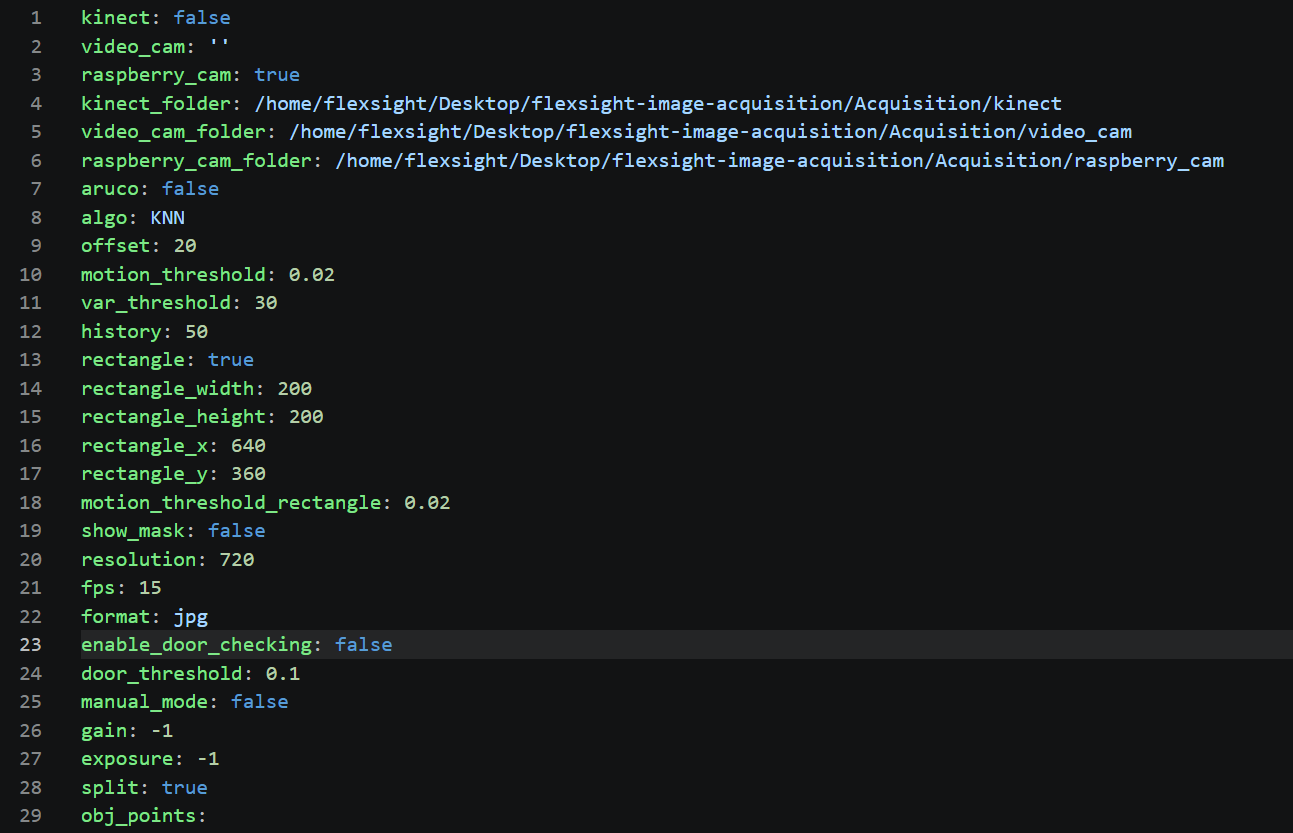
\includegraphics[width=\textwidth]{images/YAML.png}
    \caption{Example of the YAML configuration file used to tune the motion-triggering module without modifying the source code.}
    \label{fig:YAML_config}
\end{figure}

The same logic is reused across the two sites, but the sensing modality depends on the available hardware. In the Kinect branch, ROI-based triggering can be performed on the transformed depth image, the infrared image, or the RGB image. The transformed depth image is particularly convenient because it is substantially invariant to illumination changes. In RGB-only branches, such as the Raspberry Pi acquisition setup used at Site~2, the foreground mask is instead computed directly from the RGB stream.\cite{labby_kinect_acquisition_2026} The framework also skips an initial number of frames in order to stabilize the background model before the actual recording starts, thereby reducing false triggers caused by transient initialization artefacts.

When the motion score exceeds the configured threshold within the selected ROI, the current frame is written to disk together with the modality-specific data associated with the active sensor. In the Kinect setup, the acquisition stage stores RGB, depth, infrared, and mask data. The RGB frames are used for automatic labelling and detector training, whereas the aligned depth data are used to develop and validate the volume-estimation workflow. In the Raspberry Pi setup, the stored outputs are instead the RGB frame and the associated foreground mask, and these data are later used to train the detector and support the downstream bread-analysis pipeline.\cite{labby_kinect_acquisition_2026,labby_thesis_repo_2026} In order to better subdivide the events, the codebase also supports the automatic creation of timestamped folders when motion starts, so that separate acquisition sessions can be organized without manual intervention.\cite{labby_kinect_acquisition_2026}
\newpage
\subsubsection{Data Management and Robustness}
Since the local storage capacity of the embedded devices is limited, the acquisition framework also includes a flushing mechanism that reacts to low-space conditions. When enabled, this mechanism pauses the acquisition logic and allows the oldest files to be transferred to an external SSD, thereby freeing local space for new data.\cite{labby_kinect_acquisition_2026} This feature is particularly useful during long autonomous campaigns, where the amount of generated data can quickly exceed the internal storage capacity of the device.

\begin{figure}[h]
    \centering
    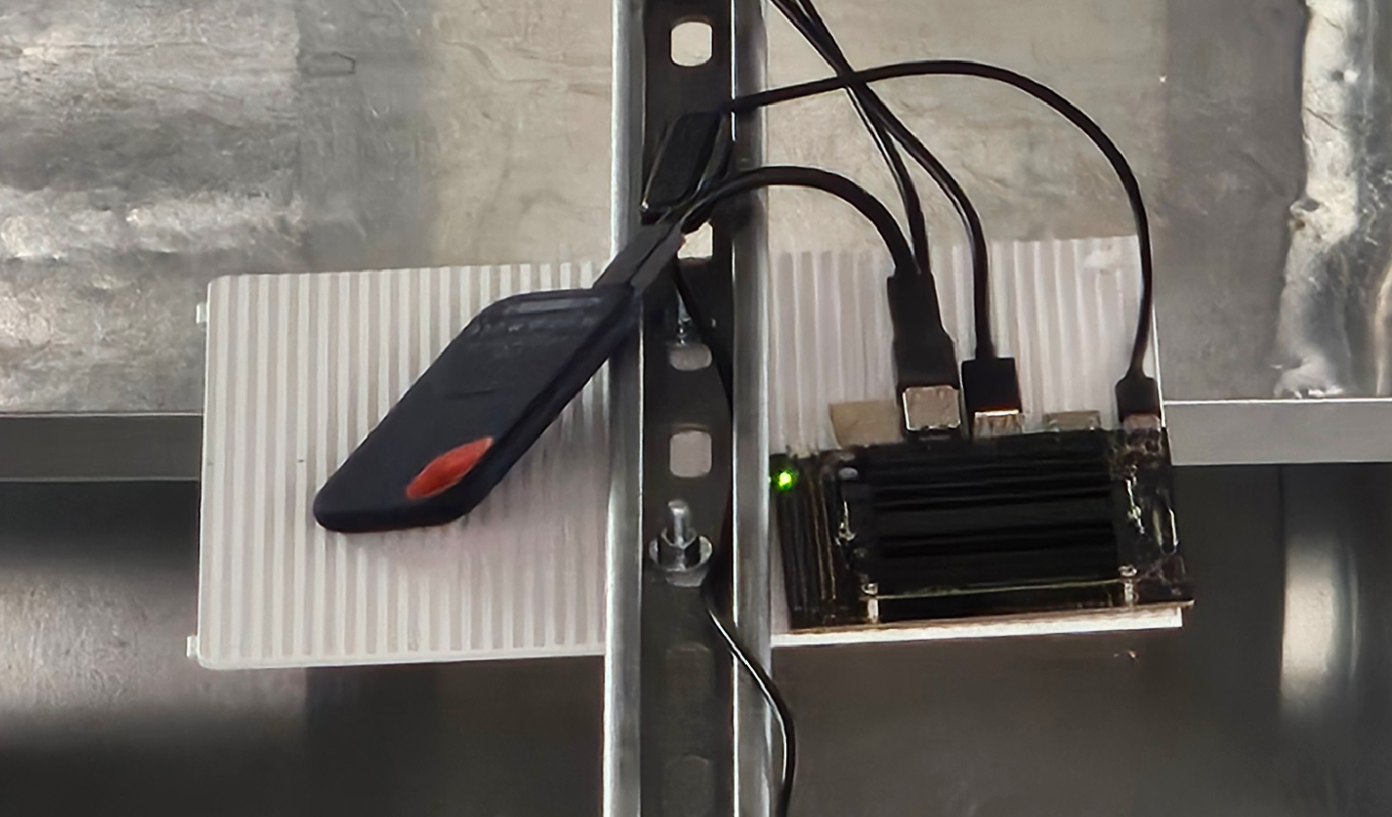
\includegraphics[width=0.5\textwidth]{images/ssd.PNG}
    \caption{Jetson Nano with the external SSD used for data flushing during long acquisition campaigns.}
    \label{fig:SSD_flushing}
\end{figure}

To further increase robustness, the acquisition scripts can be launched automatically at startup through system services or desktop autostart entries, so that the data-collection process can resume after power interruptions or device reboots without requiring manual intervention.\cite{labby_kinect_acquisition_2026,systemd_service_2026} As discussed in Chapter~1, this aspect was essential for ensuring continuity during two-week acquisition campaigns in an industrial environment.

Overall, this motion-triggered acquisition strategy proved particularly suitable for long autonomous campaigns, because it reduces redundant storage while preserving the samples that are most informative for the subsequent labelling and training stages. At the same time, the framework remains modular enough to support different sensors and acquisition modes without requiring a complete redesign of the system.\cite{labby_kinect_acquisition_2026}


\section{Automatic Labelling}
% !TeX root = ../../tesi.tex

To reduce the manual effort required to annotate the collected datasets and to speed up the work, an automatic labelling strategy based on Language Segment-Anything (Lang-SAM) was adopted on an offline workstation.\cite{medeiros_luca-medeiroslang-segment-anything_2026} This choice is consistent with the overall workflow adopted in this thesis, since annotation generation is computationally more suitable for a higher-resource environment than the embedded devices used for data acquisition and online inference. Lang-SAM is a zero-shot framework that combines text-guided localization and segmentation, making it possible to obtain object masks or bounding boxes directly from natural-language prompts describing the target product.

In the implemented workflow, prompts referring to dough balls or bread loaves are used to detect the products in the acquired frames. The generated bounding boxes are then manually checked for correctness and exported in a detector-compatible annotation format, in this case the COCO dataset format. This procedure provides a common labelling pipeline for both sites, significantly reduces manual annotation time, and keeps the detector-training stage consistent across the two datasets.\cite{labby_thesis_repo_2026}
\begin{figure}[h]
    \centering
    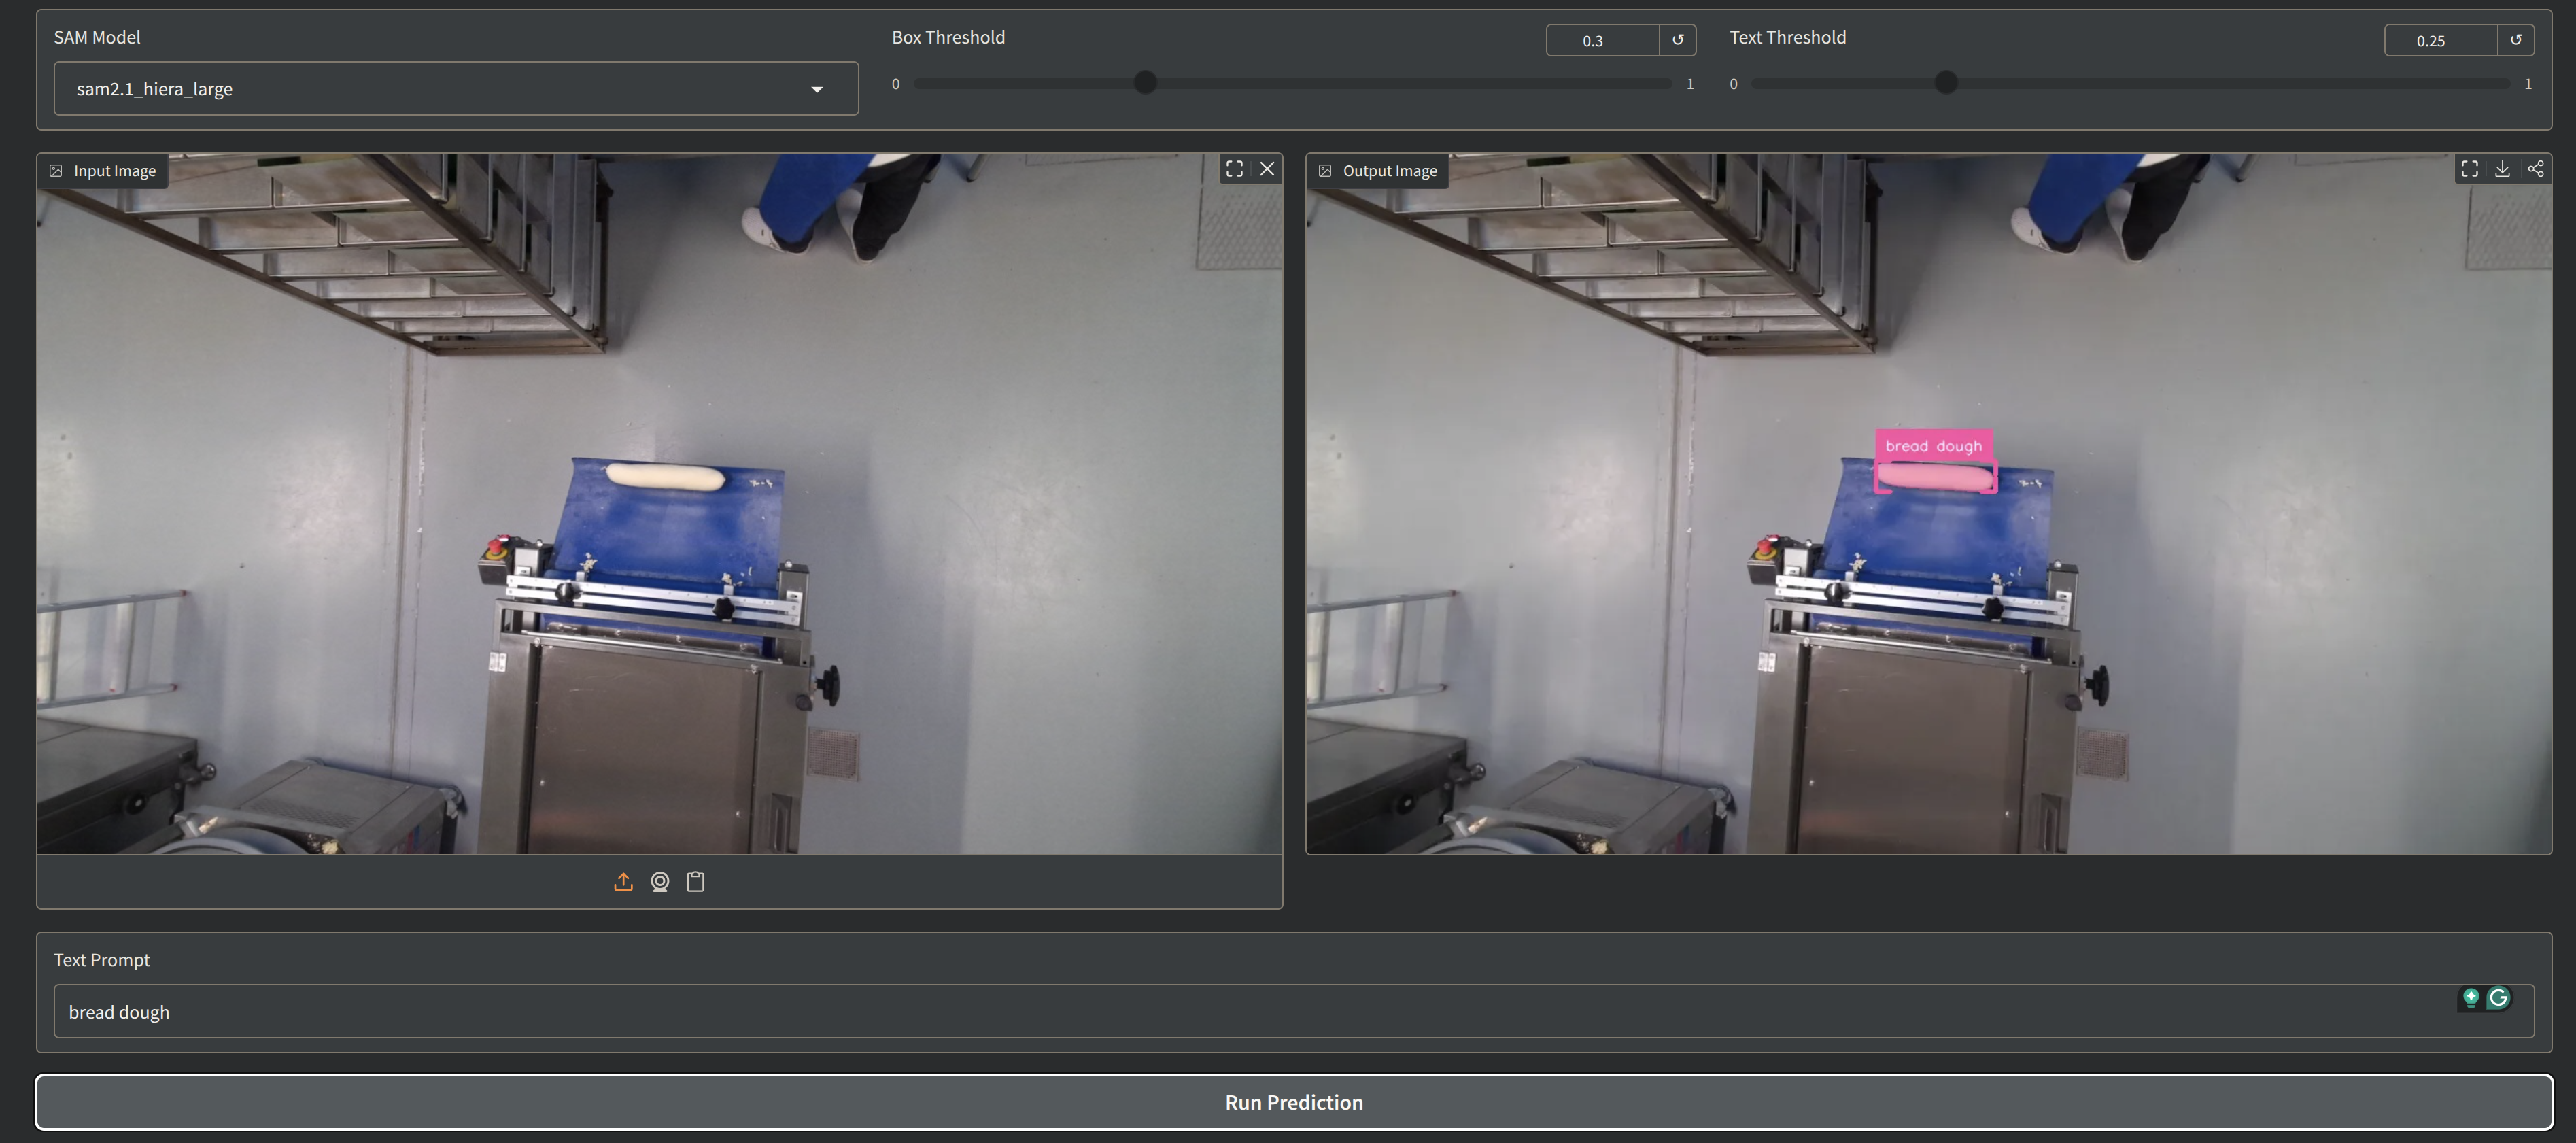
\includegraphics[width=\textwidth]{images/Useful-photos/Screenshots/Screenshot from 2026-02-23 17-16-41.png}
    \caption{Example of automatic labelling using Lang-SAM. The left image shows the original frame with a natural-language prompt describing the target product (e.g., "dough ball" or "bread loaf"). The right image displays the resulting segmentation mask and bounding box generated by Lang-SAM. This approach significantly reduces manual annotation effort while maintaining consistency across datasets.}
    \label{fig:LangSAM_labelling}
\end{figure}


\section{DEIMv2 Training}
% !TeX root = ../../tesi.tex

After acquisition and automatic labelling, the DEIMv2 detector is trained offline on a workstation with higher computational resources than the embedded devices used on site.\cite{huang_real-time_2026} This choice is necessary because the edge platforms are intended primarily for acquisition and online inference, whereas detector training requires longer optimization runs and larger memory budgets.
The automatically labelled images and the corresponding COCO-format annotations described in the previous section are used to build the detector datasets, which are then partitioned into training, validation, and test subsets with an 80/10/10 split.

Although the two industrial sites lead to different downstream tasks, the role of DEIMv2 is the same in both cases: the network must localize the product instances and provide reliable regions of interest for the subsequent processing stages. The model is therefore trained on two site-specific datasets, while preserving the same detector architecture and the same general training logic.\cite{labby_thesis_repo_2026} At Site~1, the detected regions are associated with aligned depth data and used for volumetric reconstruction. At Site~2, they are converted into loaf crops that feed the anomaly-detection branch. In this sense, DEIMv2 constitutes, together with the automatic labelling stage, the common detection layer of the overall framework.

During training, the optimization dynamics are monitored through TensorBoard, and the final checkpoint is selected according to the lowest validation loss observed during the training schedule. The resulting curves and the quantitative detection metrics obtained on the two datasets are discussed in Chapter~5.

Once the training stage is completed, the selected checkpoint is redeployed on the embedded target platform and becomes the detector used during online acquisition and inference. This offline-to-online transition allows the computationally demanding optimization stage to remain separated from the lightweight deployment stage, while preserving a consistent detection pipeline across the two monitoring sites.\cite{labby_thesis_repo_2026}


\section{Feature Extraction and Quality Assessment}
% !TeX root = ../../tesi.tex

\subsection{Site 1: Volume Estimation}
The volume-estimation branch at Site~1 was developed through several increasingly refined workflows. A first baseline estimated volume by computing a convex hull directly from the points contained within each detected bounding box. However, this bounding-box-only approximation was not sufficiently accurate, because the selected region also included non-dough elements that biased the reconstructed geometry. Subsequent variants therefore introduced an explicit segmentation stage before volumetric reconstruction. SAM \cite{kirillov_segment_2023} was first explored as a foreground-segmentation tool and produced very accurate masks, but its computational cost proved too high for the intended workflow, whose long-term goal is deployment on edge devices. The final implementation therefore relies on a more efficient pipeline based on color clustering, refined through depth-based background subtraction and followed by axis-based 3D completion.\cite{labby_thesis_repo_2026}

\subsubsection{Detection Filtering}
Before volumetric processing, the detections are filtered so as to retain only the most reliable samples. In particular, a dedicated preprocessing stage builds a filtered detection cache by keeping only images containing a single valid dough-ball detection inside a predefined ROI polygon. This step reduces ambiguities caused by multiple simultaneous objects, spurious detections near the borders of the acquisition area, or colliding dough balls, all of which can be problematic for the subsequent volume-estimation stage.

This filtering stage was introduced because the main aim of this part of the thesis is to analyze the consistency of the volume-estimation algorithms on a well-defined set of samples, rather than to evaluate the robustness of the detector under crowded or ambiguous conditions. According to the nominal operating conditions of the line, multiple dough balls should not be present simultaneously on the output table; frames exhibiting such cases were therefore treated as outliers and excluded from the analysis.
\newpage

\subsubsection{Reference Table Modelling}
The supporting table is modelled separately from a set of empty-scene acquisitions. These depth images are aggregated through a robust median operation in order to produce a reference depth background for the table. The resulting model is stored as a numerical depth map for subsequent computations and can also be exported as a point cloud or mesh for debugging and visualization purposes, as shown in Figure~\ref{fig:table_model}.\cite{labby_thesis_repo_2026} This reference surface is later used both to remove the support contribution from the dough point cloud and to define the geometric relation between the visible dough region and the table plane.

\begin{figure}[!htbp]
    \centering
    \begin{subfigure}[b]{0.48\textwidth}
        \centering
        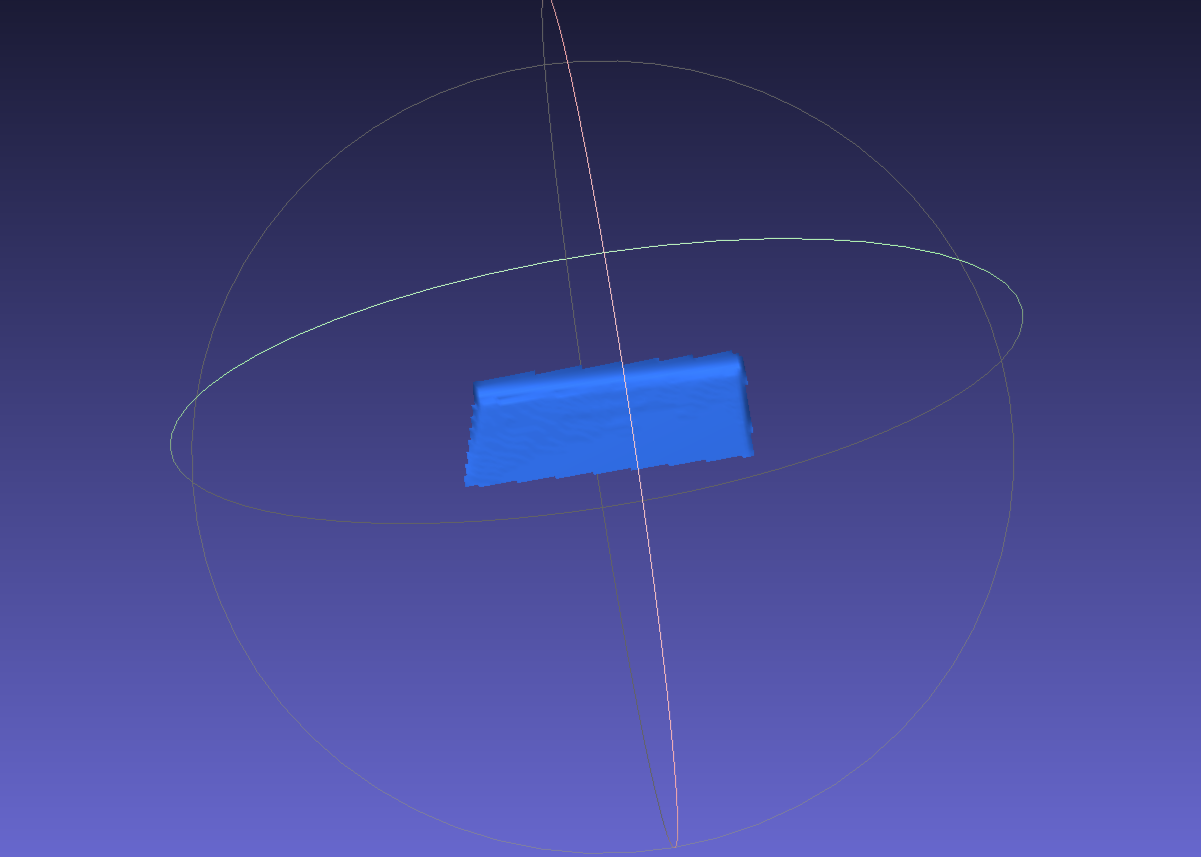
\includegraphics[width=\linewidth]{images/Useful-photos/Screenshots/BG_table.png}
        \caption{Front view}
    \end{subfigure}
    \hfill
    \begin{subfigure}[b]{0.48\textwidth}
        \centering
        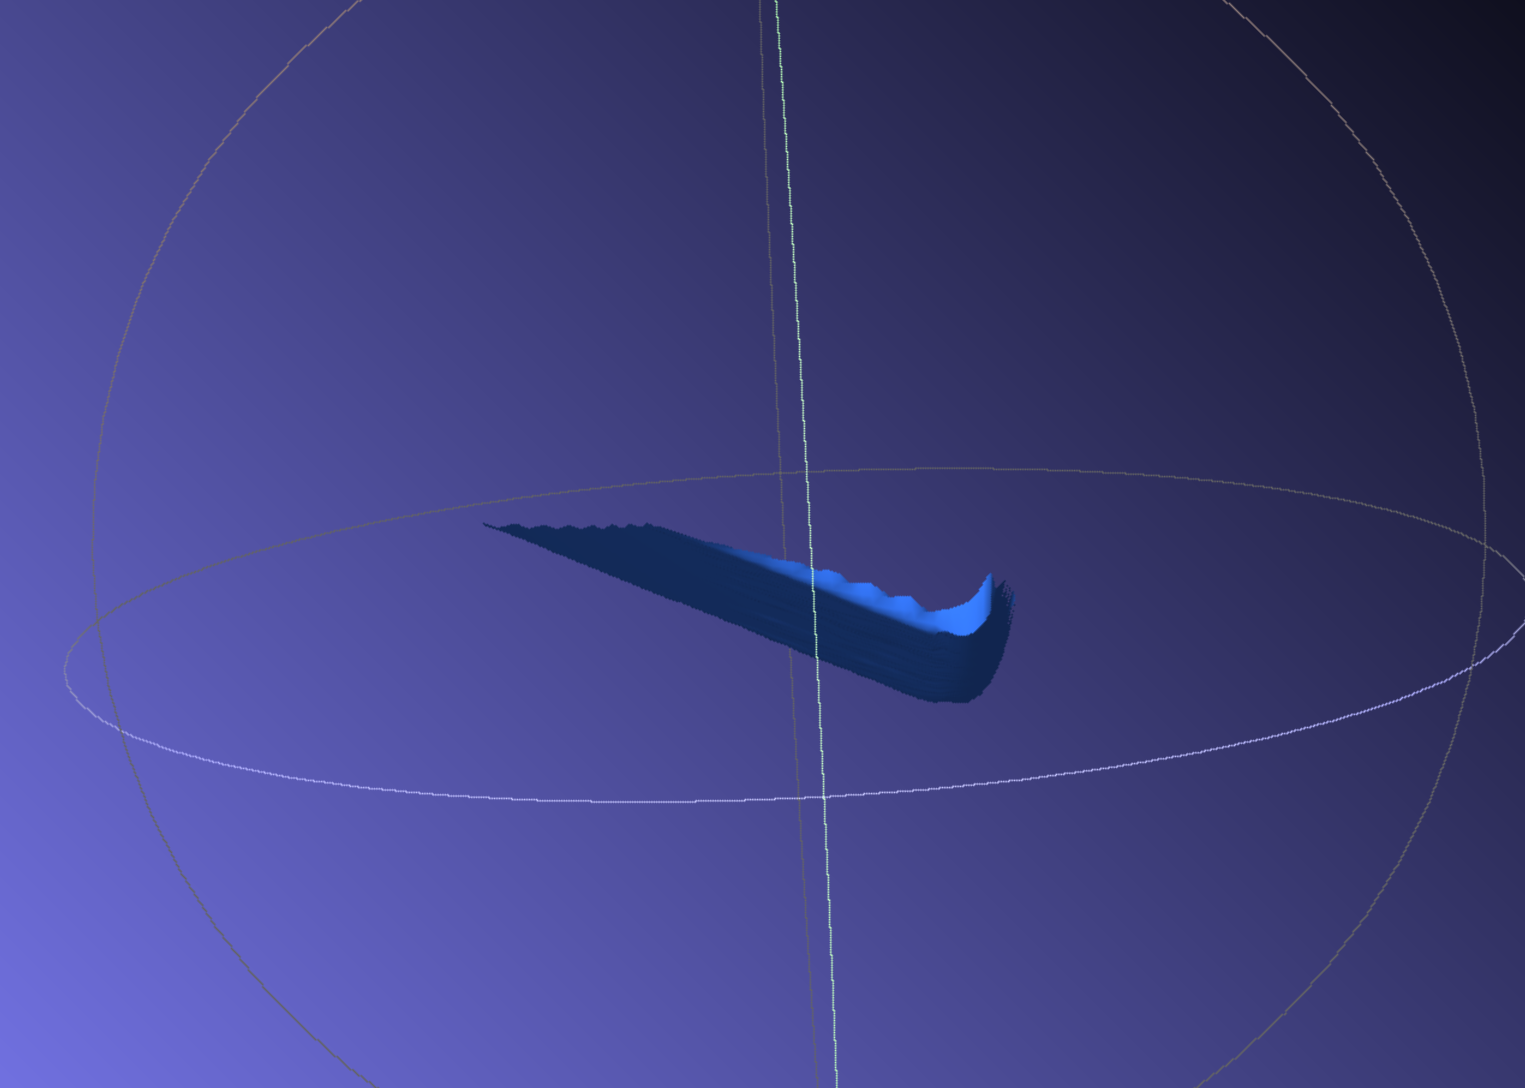
\includegraphics[width=\linewidth]{images/Useful-photos/Screenshots/BG_table2.png}
        \caption{Side view}
    \end{subfigure}
    \caption{Reference table model reconstructed from empty-scene depth acquisitions.}
    \label{fig:table_model}
\end{figure}

\subsubsection{Foreground Extraction and Point-Cloud Generation}
Once a dough-ball detection has been selected, the corresponding RGB bounding box is associated with the aligned depth image through the Kinect calibration and reprojection pipeline. Because the RGB and depth streams of the Azure Kinect have different intrinsic parameters, extrinsic relationships, and fields of view, a dedicated reprojection and alignment stage was implemented using the calibration data provided by the Azure Kinect SDK and accessed in Python through the \textit{pyKinectAzure} interface.\cite{microsoft_azure-kinect-sensor-sdk_2026,gorordo_fernandez_pykinectazure_2026} This stage makes it possible to map the RGB detections onto the corresponding depth coordinates and therefore to associate each RGB bounding box with the correct 3D measurements.

\begin{figure}[h]
    \centering
    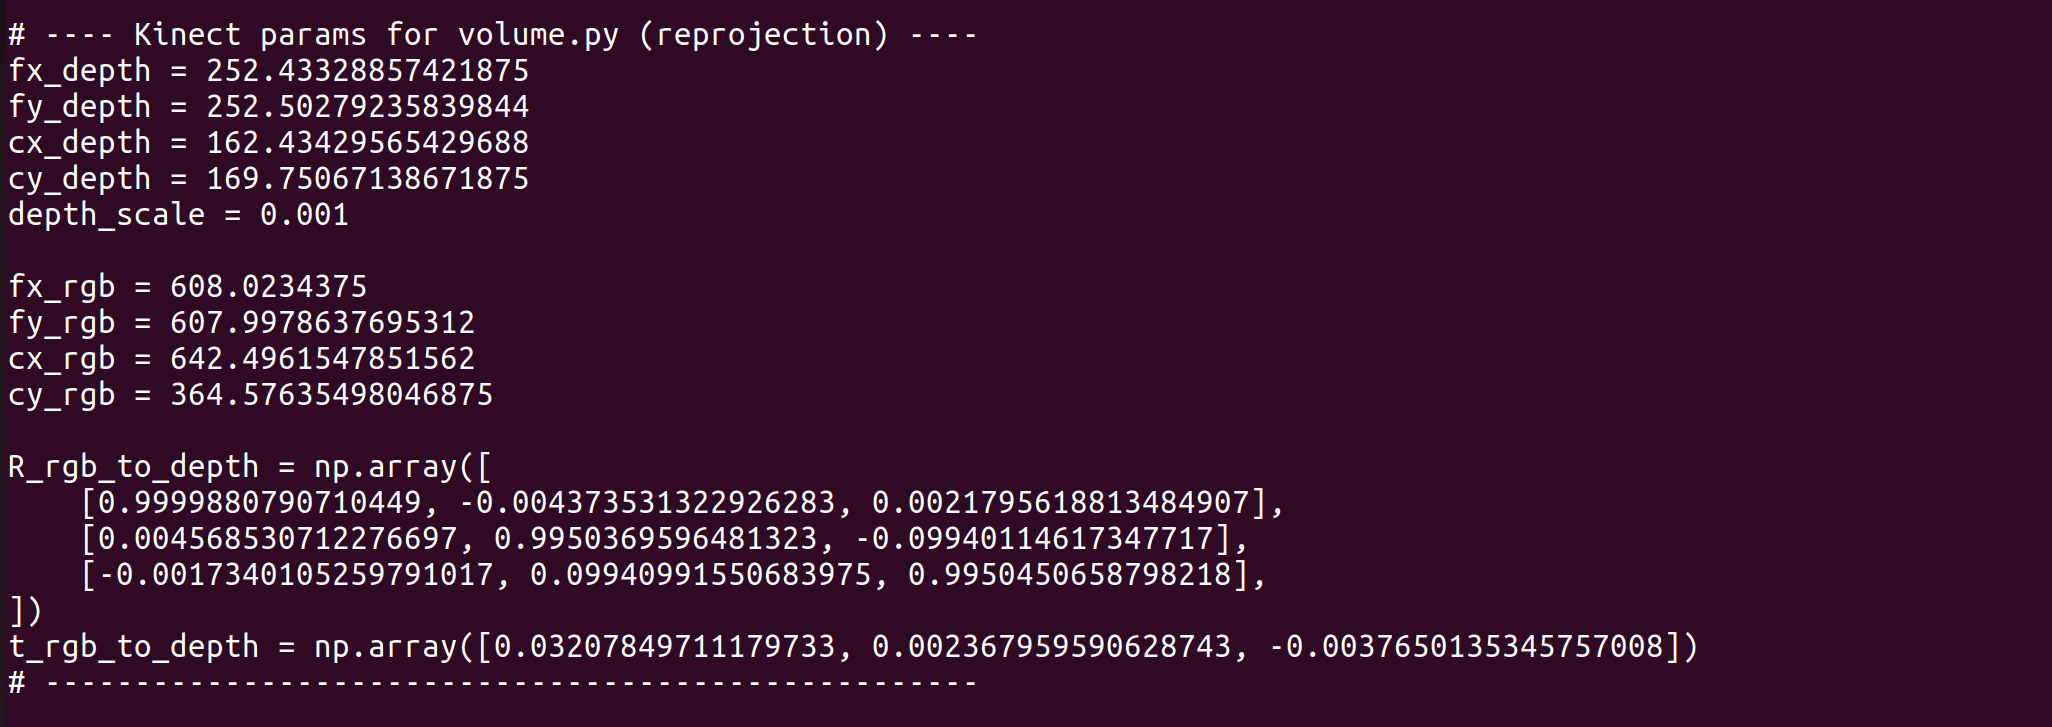
\includegraphics[width=0.80\textwidth]{images/Reprojection_param.png}
    \caption{Kinect reprojection parameters. The figure shows the RGB and depth intrinsic parameters, as well as the extrinsic transformation between the two sensors, which are used to align the RGB detections with the depth data.}
    \label{fig:reprojection_parameters}
\end{figure}

The local 3D point cloud is then obtained from the aligned depth pixels by means of the standard pinhole camera model:

\begin{equation}
X = \frac{(u - c_x) \cdot Z}{f_x}, \quad
Y = \frac{(v - c_y) \cdot Z}{f_y}, \quad
Z = D(u,v)
\end{equation}

where $(u,v)$ are the pixel coordinates, $D(u,v)$ is the depth value, $(c_x, c_y)$ are the principal-point coordinates, and $f_x$ and $f_y$ are the focal lengths expressed in pixel units.
\\
The implementation supports different segmentation modes, namely \texttt{sam}, \texttt{bbox}, and \texttt{color}.\cite{labby_thesis_repo_2026} These modes are configurable through the experiment configuration file, whereas the workflow adopted for the main experiments initializes the foreground in \texttt{color} mode and then refines it in depth (\texttt{color\_then\_depth}). More specifically, a central rectangular seed (shown in yellow in Figure~\ref{fig:color_segmentation}) is first derived from each detection, and the clustering stage can also be extended by a configurable percentage beyond the predicted bounding box so as to remain robust even when the detector localization is not perfectly tight. The color-based stage suppresses the blue background, constrains the admissible lightness range, optionally performs adaptive clustering in the \textsc{Lab} color space, and can recover dark dough regions that would otherwise be missed by a purely brightness-based filter.\cite{labby_thesis_repo_2026}

\begin{figure}[H]
    \centering
    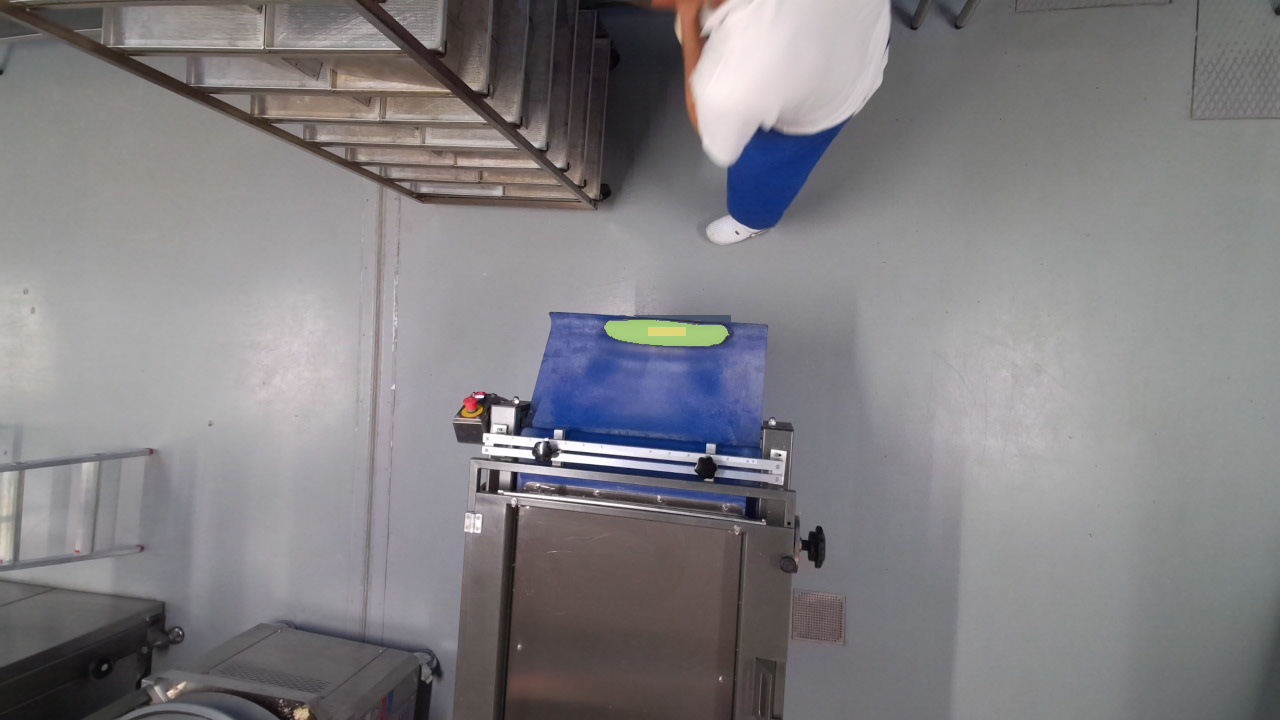
\includegraphics[width=0.70\textwidth]{images/Useful-photos/color_segmentation.png}
    \caption{Example of the color-based segmentation stage. The dough point cloud is shown in green, filtered points are highlighted in red, the seed rectangle is shown in yellow, and the background region excluded by clustering is shown in blue.}
    \label{fig:color_segmentation}
\end{figure}

In an earlier version of the workflow, this clustering step was not yet present; it was introduced later because it produced a cleaner foreground estimate before depth refinement. The resulting mask is then projected onto the depth data and further refined through background subtraction against the precomputed table model, with additional morphological filtering to improve spatial coherence.\cite{labby_thesis_repo_2026} A practical difficulty in this stage is that the depth measurements near the border of the table, especially along its final curved portion, may exhibit singular or unstable values that make the support surface harder to filter correctly. In this respect, the two refinement stages complement each other: color clustering helps suppress unstable depth regions near the table border before they enter the volumetric estimation, whereas background subtraction removes regions that may be chromatically similar to the dough but are not geometrically consistent with the support model. This issue is also mitigated by combining an adaptive background-subtraction threshold with the distance from the reference table surface. These morphological operations remove points in the point cloud that intersect, penetrate the table model, or are closer than a certain threshold to the background, thereby enforcing a geometrically consistent foreground prior to volumetric reconstruction.

\begin{figure}[H]
    \centering
    \begin{subfigure}[b]{0.48\textwidth}
        \centering
        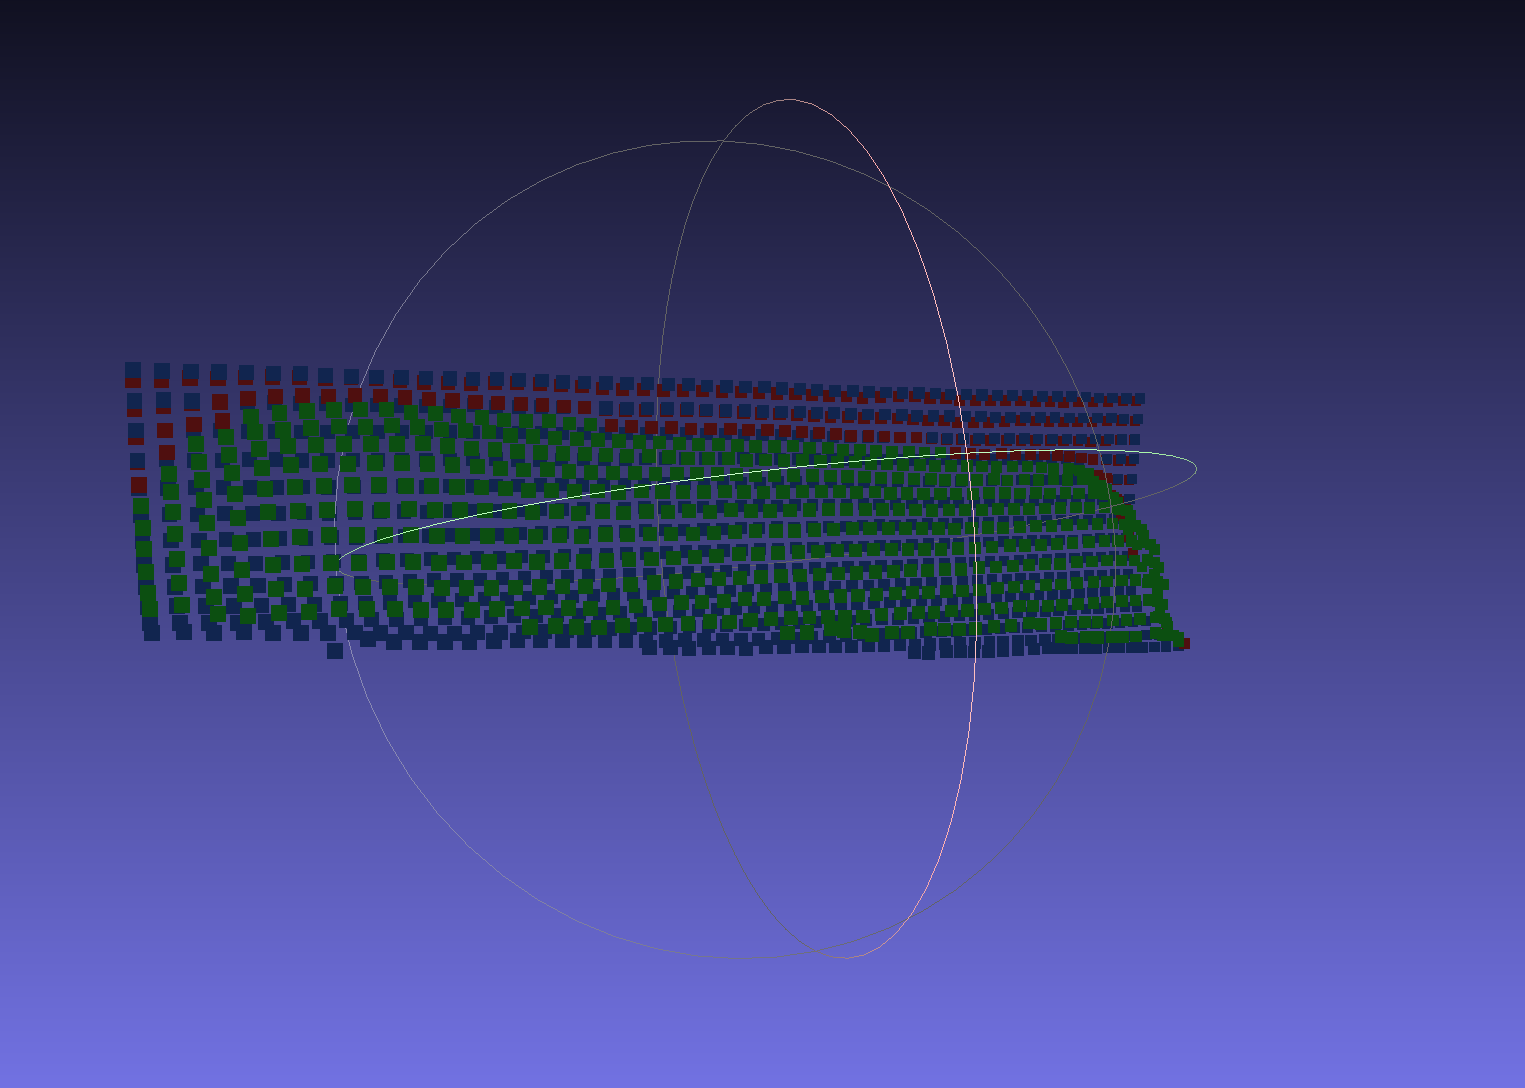
\includegraphics[width=\linewidth]{images/Useful-photos/Screenshots/erosion_front.png}
        \caption{Front view of table-collision filtering}
    \end{subfigure}
    \hfill
    \begin{subfigure}[b]{0.48\textwidth}
        \centering
        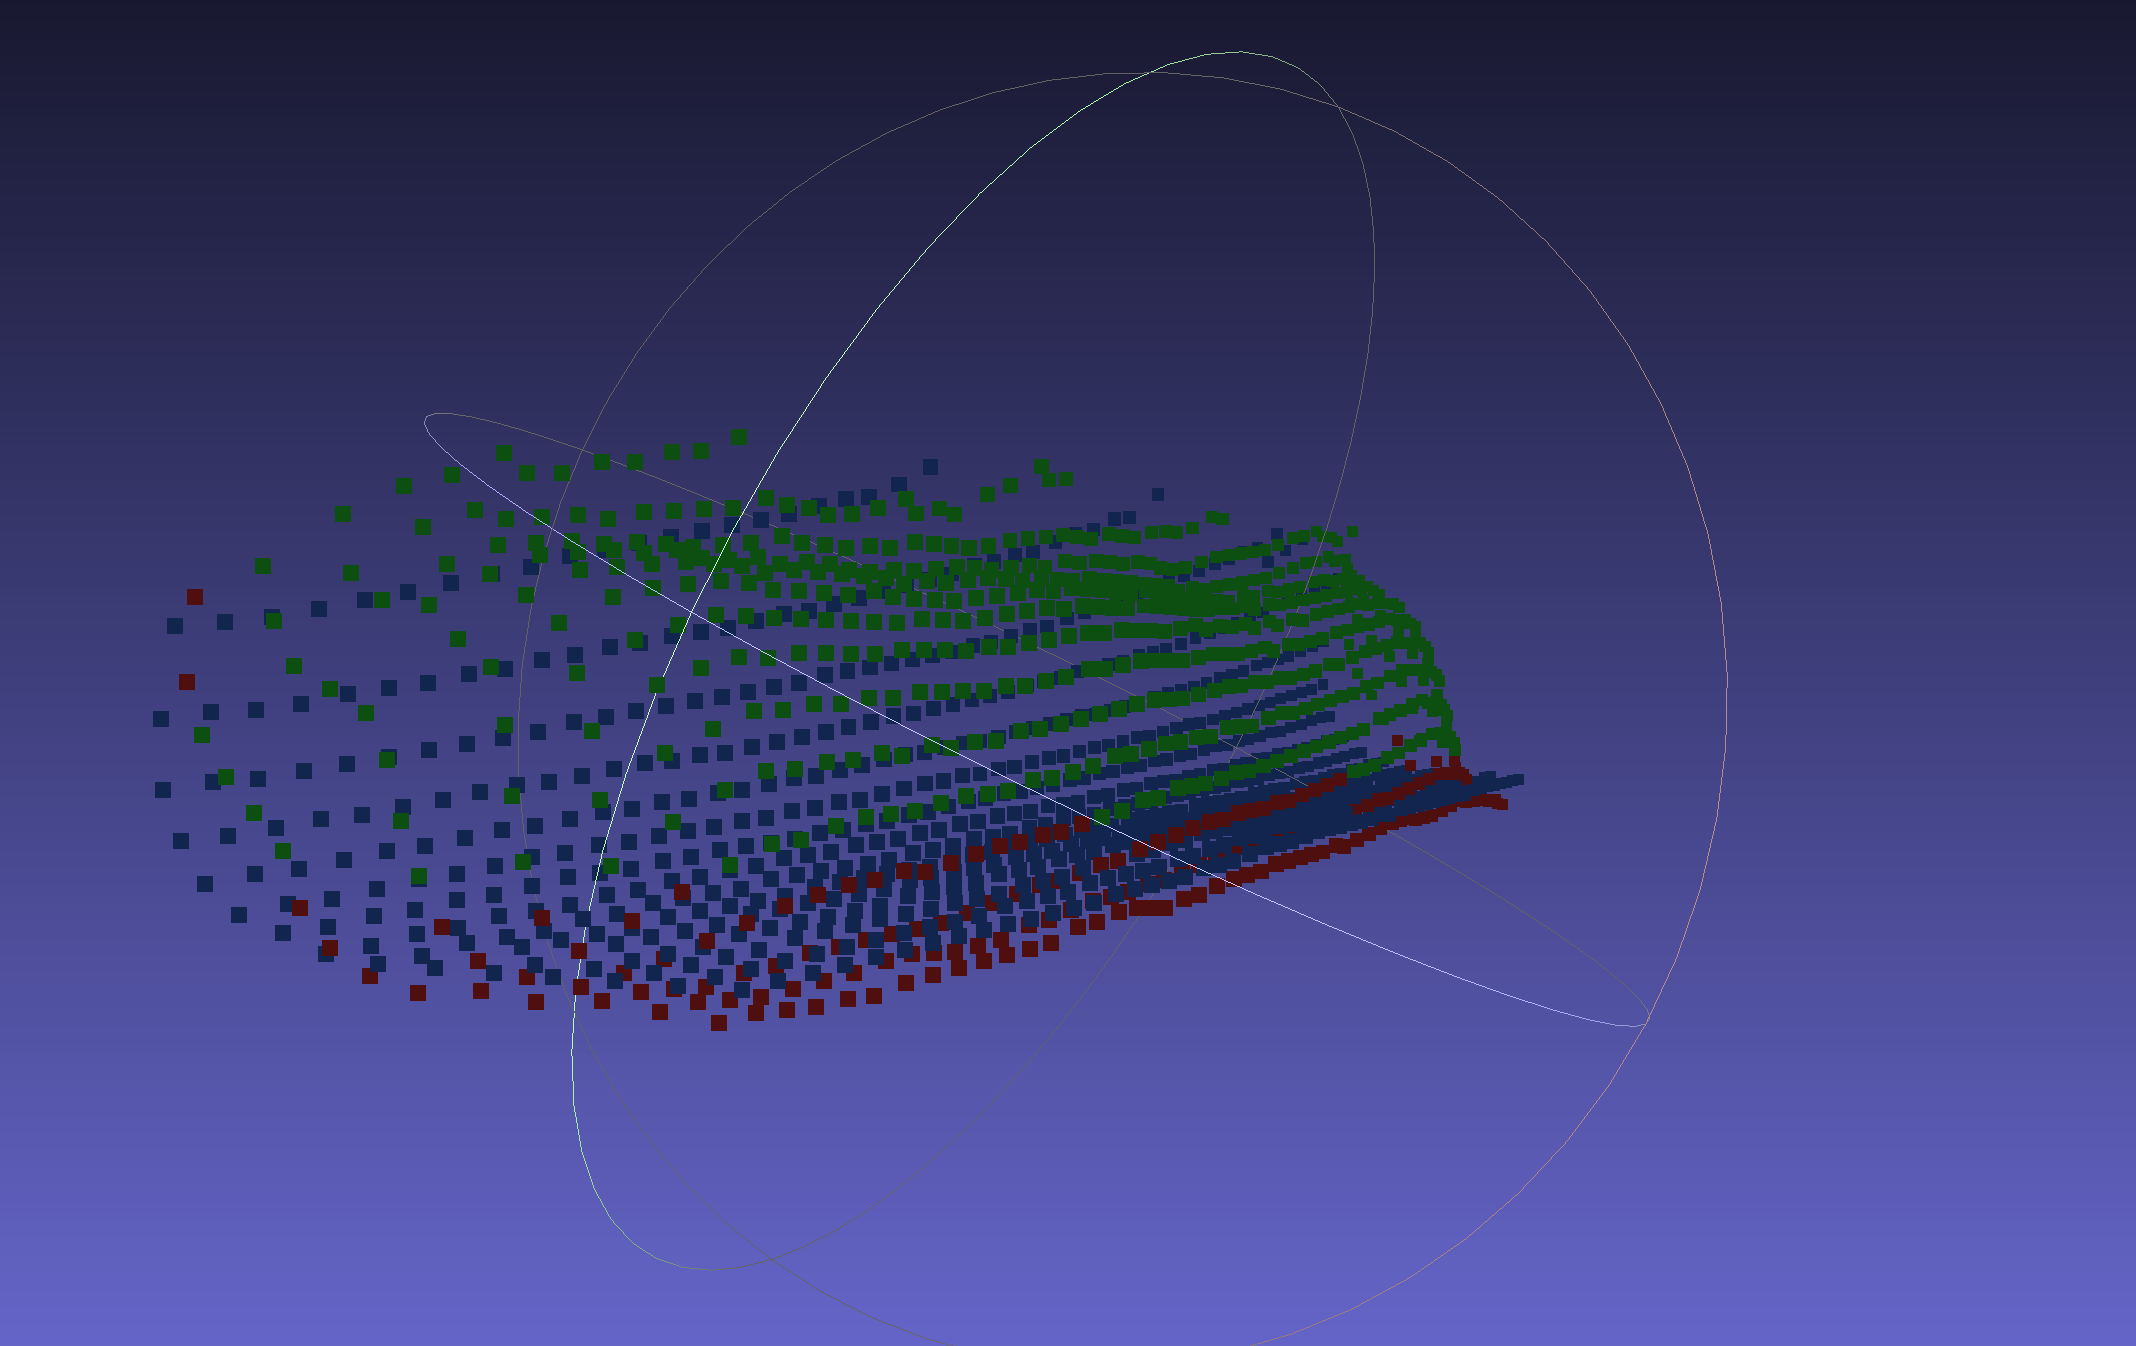
\includegraphics[width=\linewidth]{images/Useful-photos/Screenshots/erosion_side.png}
        \caption{Side view of table-collision filtering}
    \end{subfigure}
    \caption{Examples of depth-based refinement against the reference table model during foreground extraction. Red points are removed because they are too near or intersect the table model (blue points), while the remaining green points are retained as the refined dough foreground.}
\end{figure}

\begin{figure}[H]
    \centering
    \begin{subfigure}[b]{0.48\textwidth}
        \centering
        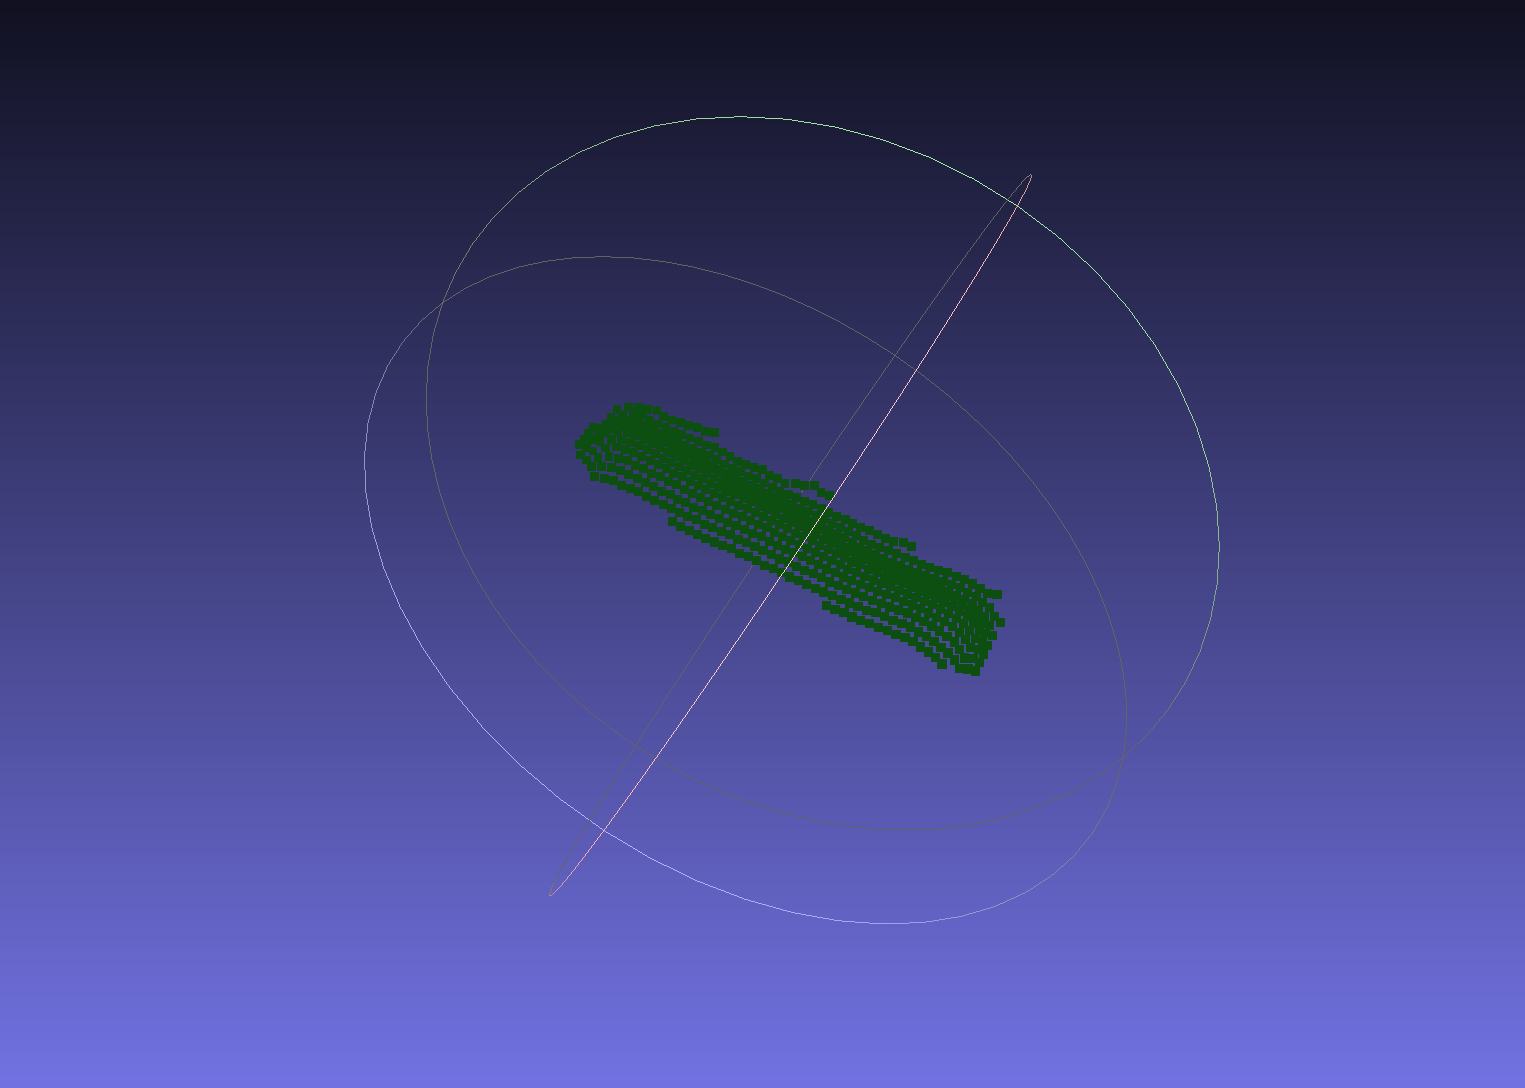
\includegraphics[width=\linewidth]{images/Useful-photos/Screenshots/erosion_result.png}
        \caption{Final foreground after refinement}
    \end{subfigure}
    \hfill
    \begin{subfigure}[b]{0.48\textwidth}
        \centering
        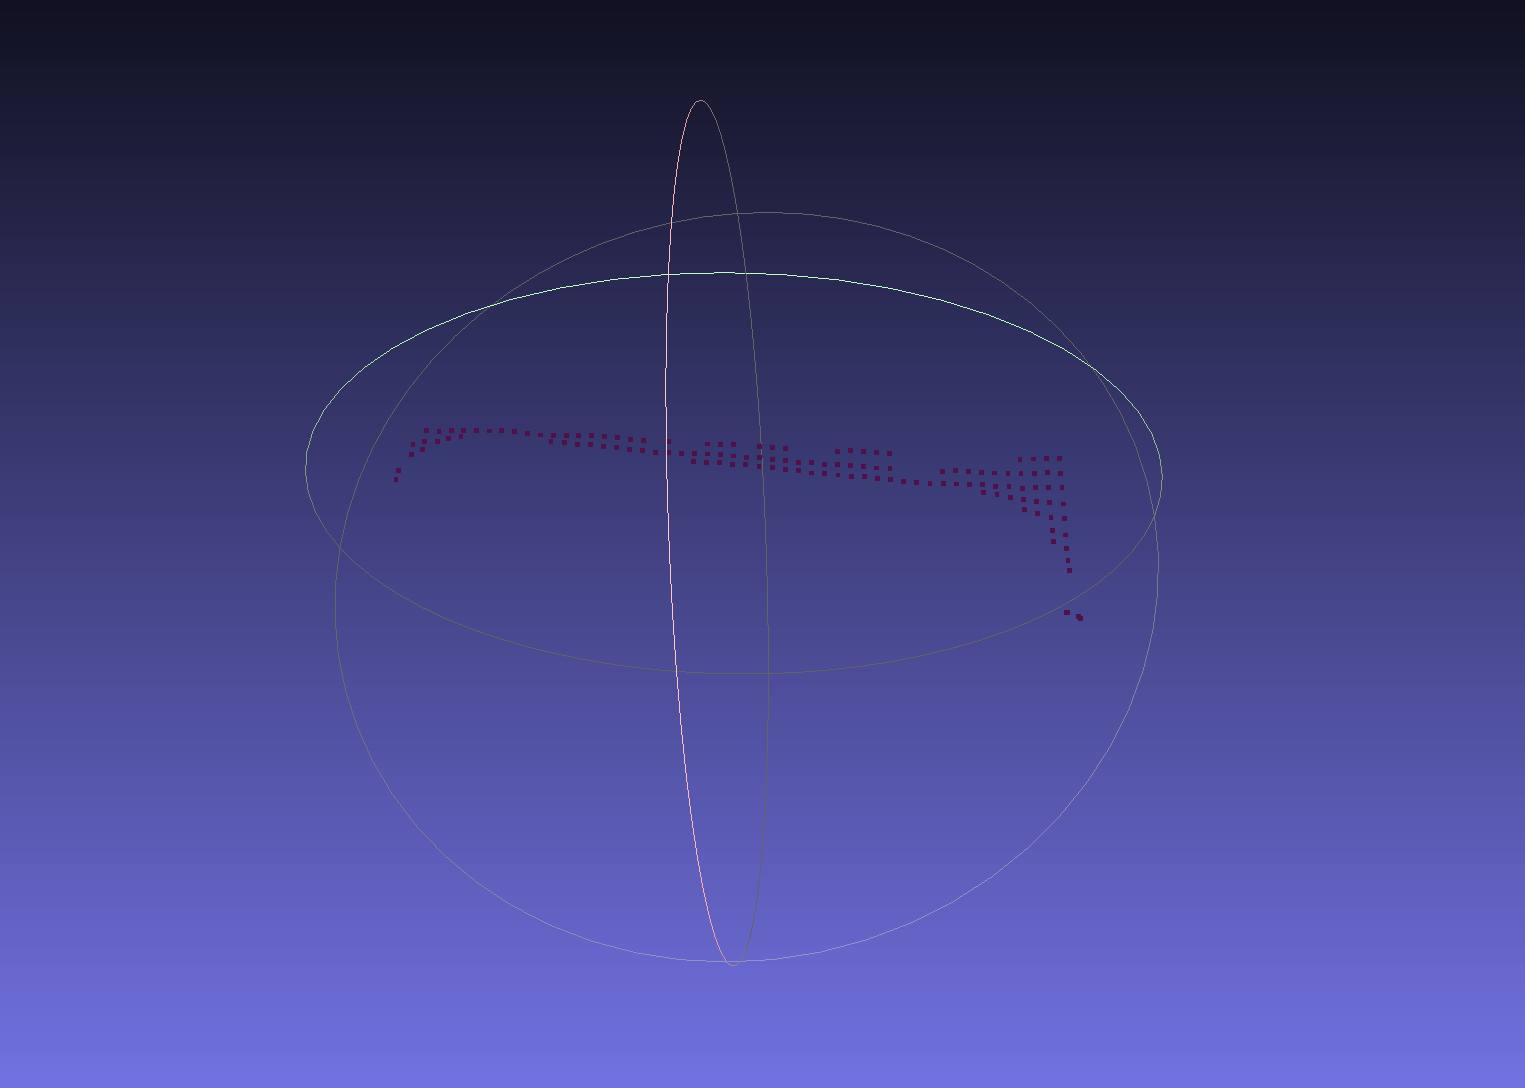
\includegraphics[width=\linewidth]{images/Useful-photos/Screenshots/erosion_removed.png}
        \caption{Points removed during refinement}
    \end{subfigure}
    \caption{Result of the depth-based refinement stage. The left image shows the final foreground after filtering, while the right image highlights the points that were removed because they were inconsistent with the reference table model. This refinement step helps to ensure that the subsequent volume estimation is based on a more accurate representation of the dough geometry.}
    \label{fig:foreground_refinement}
\end{figure}

\subsubsection{Example of Combined Clustering and Background Subtraction}
A representative example of this combined strategy is shown in Figures~\ref{fig:cluster_bgs_input} and~\ref{fig:cluster_bgs_example}. In some cases, the color-clustering stage can include a region that is chromatically similar to the dough but does not belong to the actual product surface. When the corresponding mask is compared with the reference table model, the depth-based background subtraction removes the geometrically inconsistent portion, leaving only the region that is compatible with the dough foreground. This example highlights the practical advantage of combining appearance-based clustering with geometric refinement, since the first stage provides a broad candidate region while the second suppresses portions that are incompatible with the known support geometry.

\begin{figure}[!htbp]
    \centering
    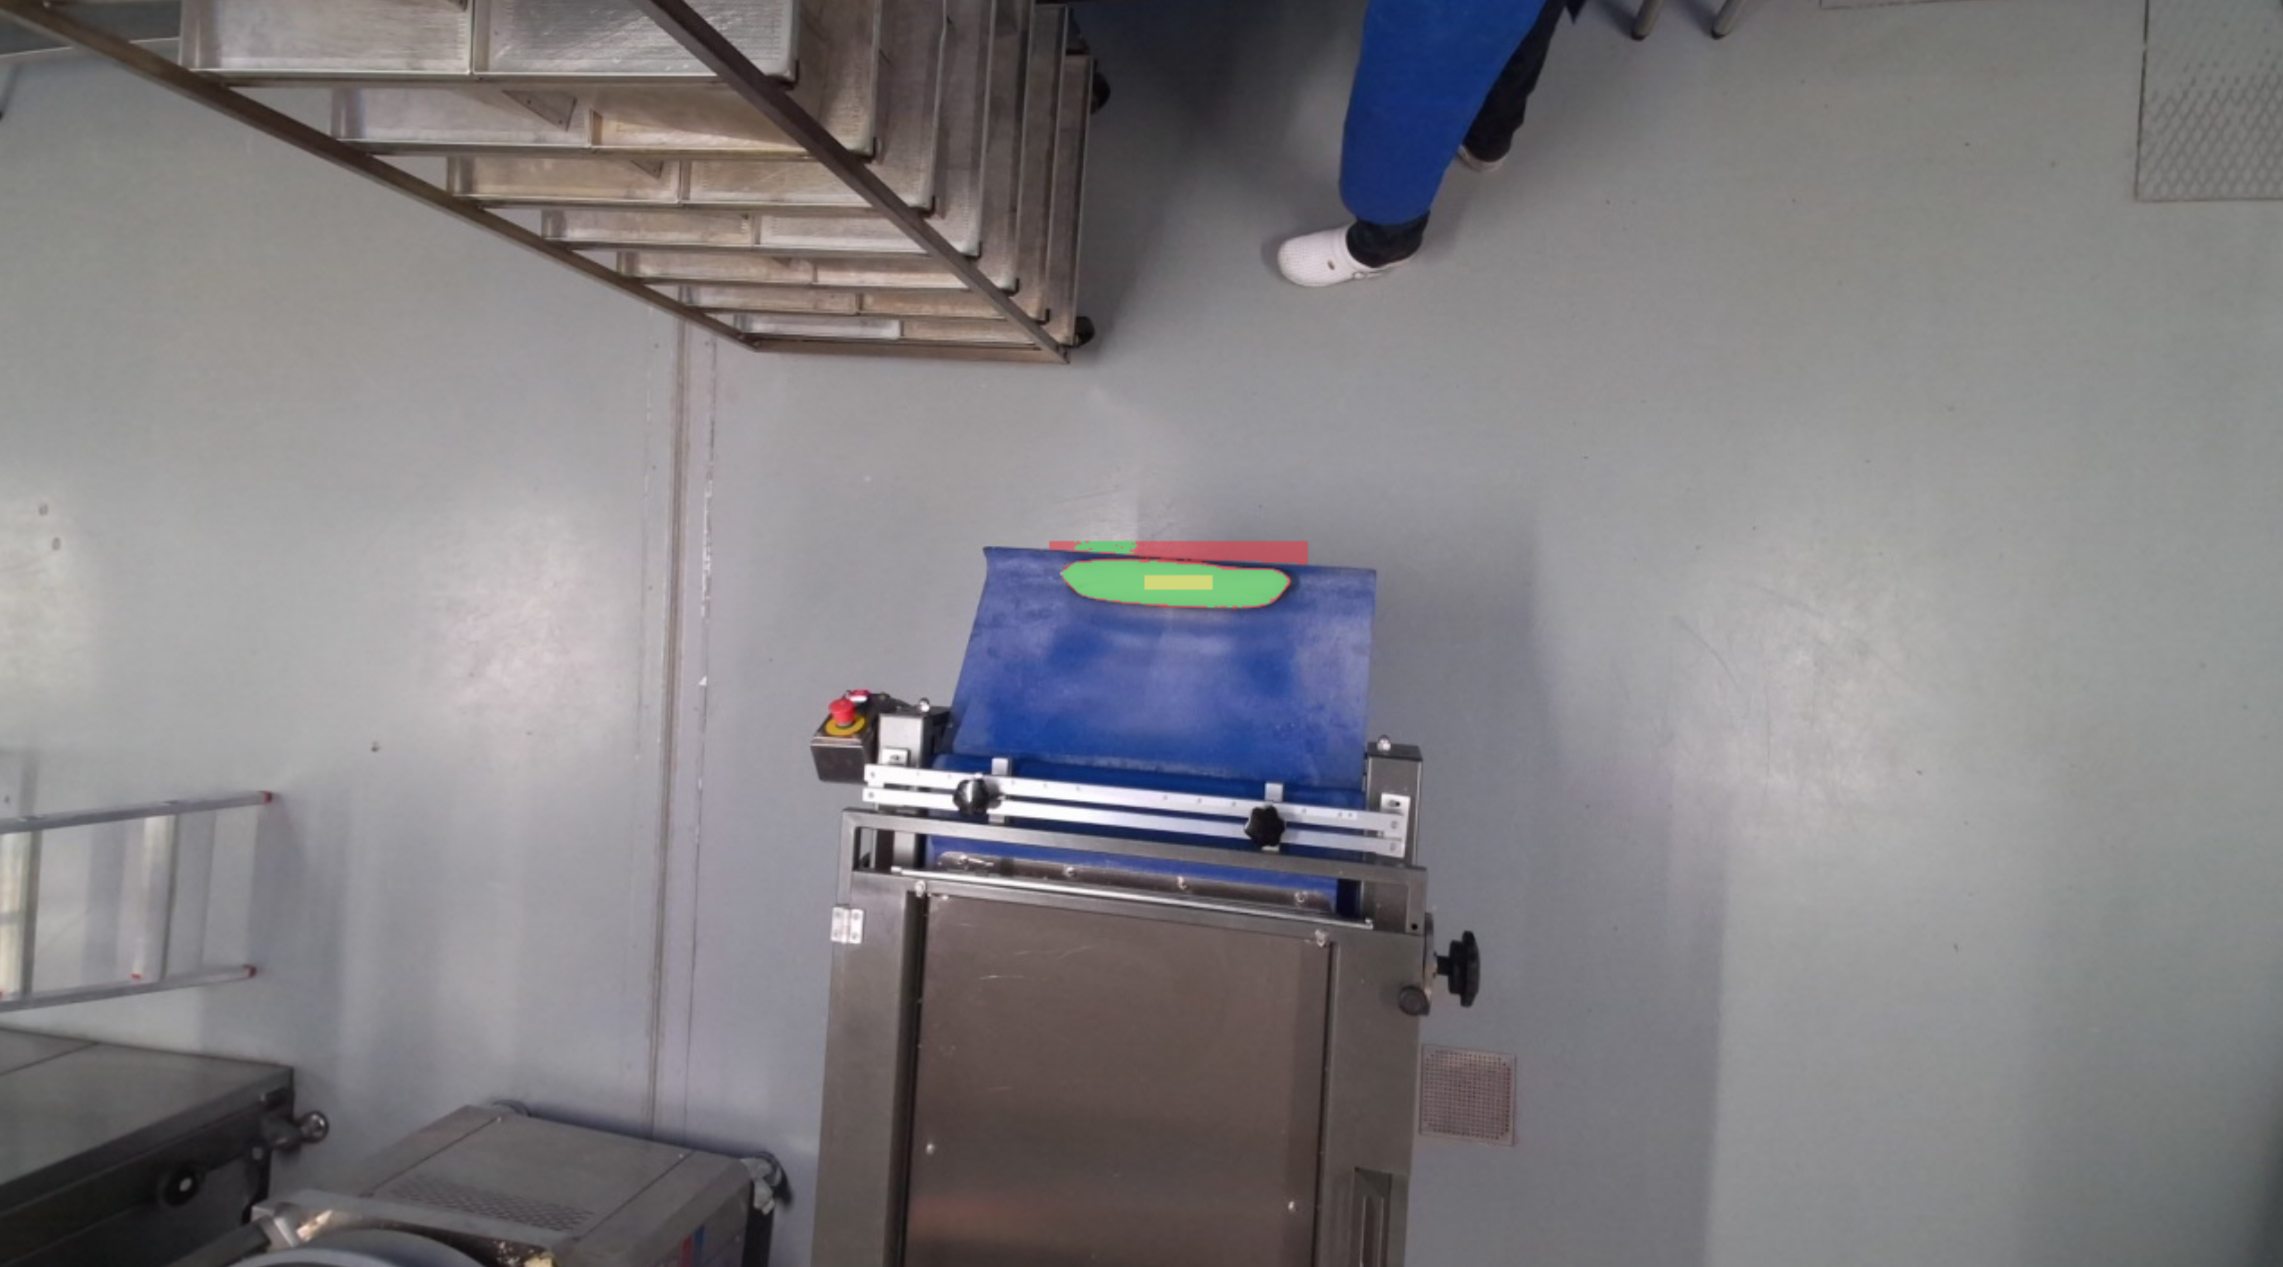
\includegraphics[width=0.58\textwidth]{images/CLuster_1.PNG}
    \caption{Example of bad clustering input. The color-based clustering stage includes an additional region in the upper-left area that is chromatically similar to the dough but does not belong to the actual product surface.}
    \label{fig:cluster_bgs_input}
\end{figure}

\begin{figure}[!htbp]
    \centering
    \begin{subfigure}[t]{0.40\textwidth}
        \centering
        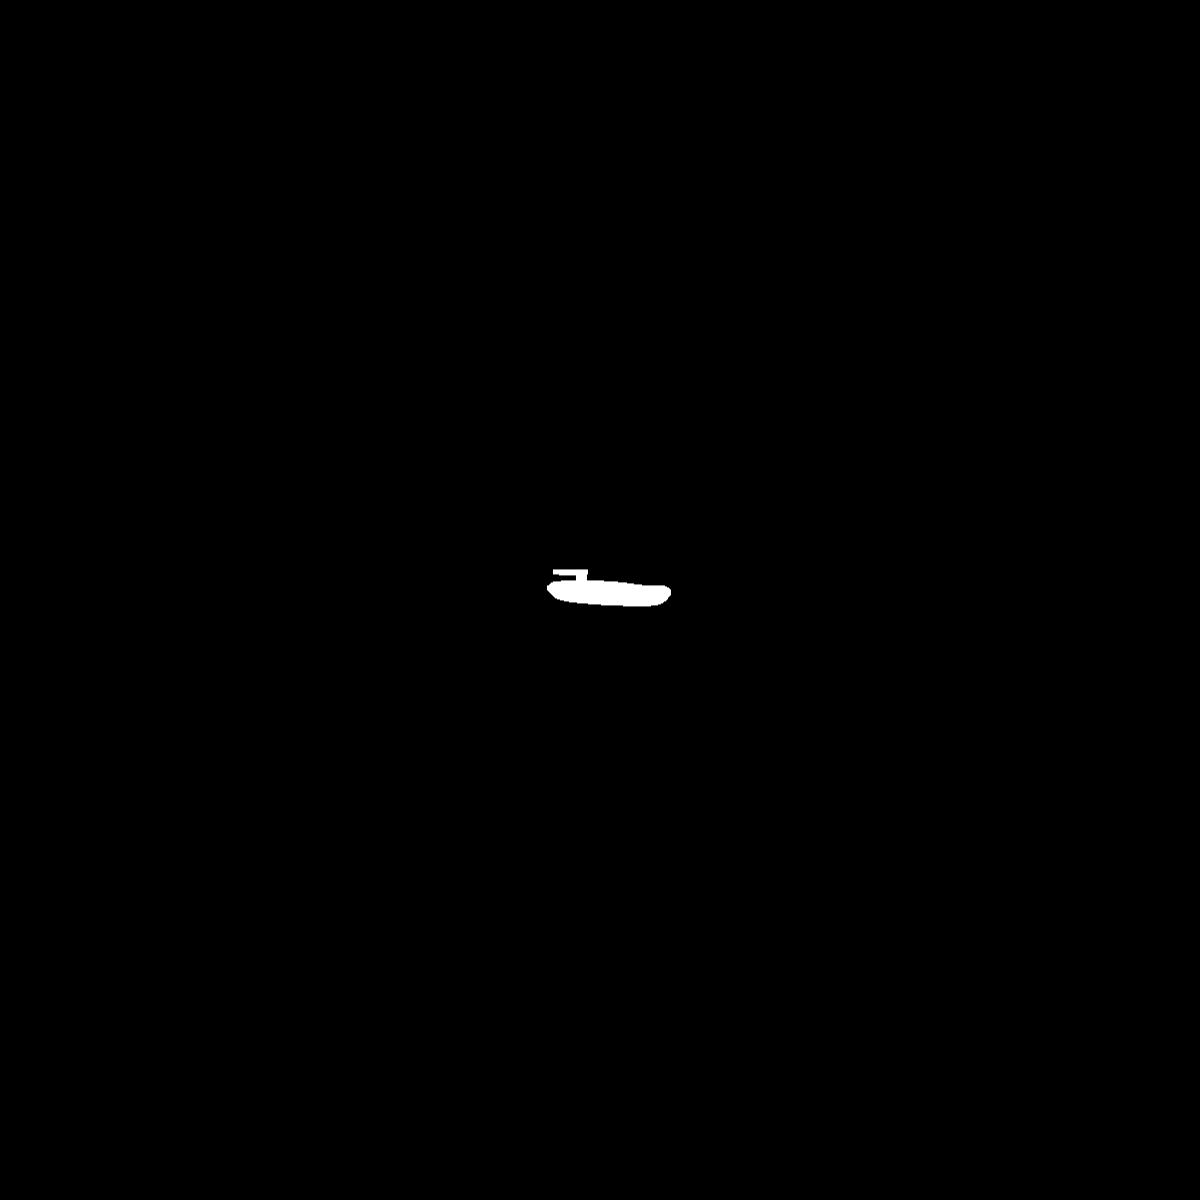
\includegraphics[width=\linewidth]{images/cluster_before.PNG}
        \caption{Mask after color clustering. Note the additional spurious region in the upper-left area}
    \end{subfigure}
    \hfill
    \begin{subfigure}[t]{0.40\textwidth}
        \centering
        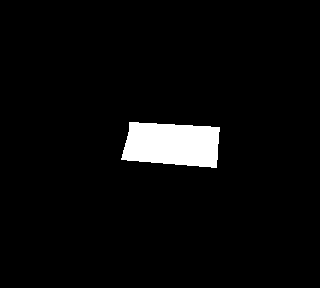
\includegraphics[width=\linewidth]{images/table_bg_table_full_mask.png}
        \caption{Reference table mask}
    \end{subfigure}

    \vspace{0.5em}

    \begin{subfigure}[t]{0.40\textwidth}
        \centering
        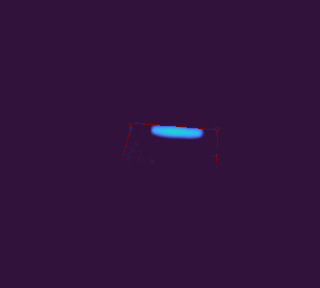
\includegraphics[width=\linewidth]{images/cluster_mid.png}
        \caption{Cluster compared with table model}
    \end{subfigure}
    \hfill
    \begin{subfigure}[t]{0.40\textwidth}
        \centering
        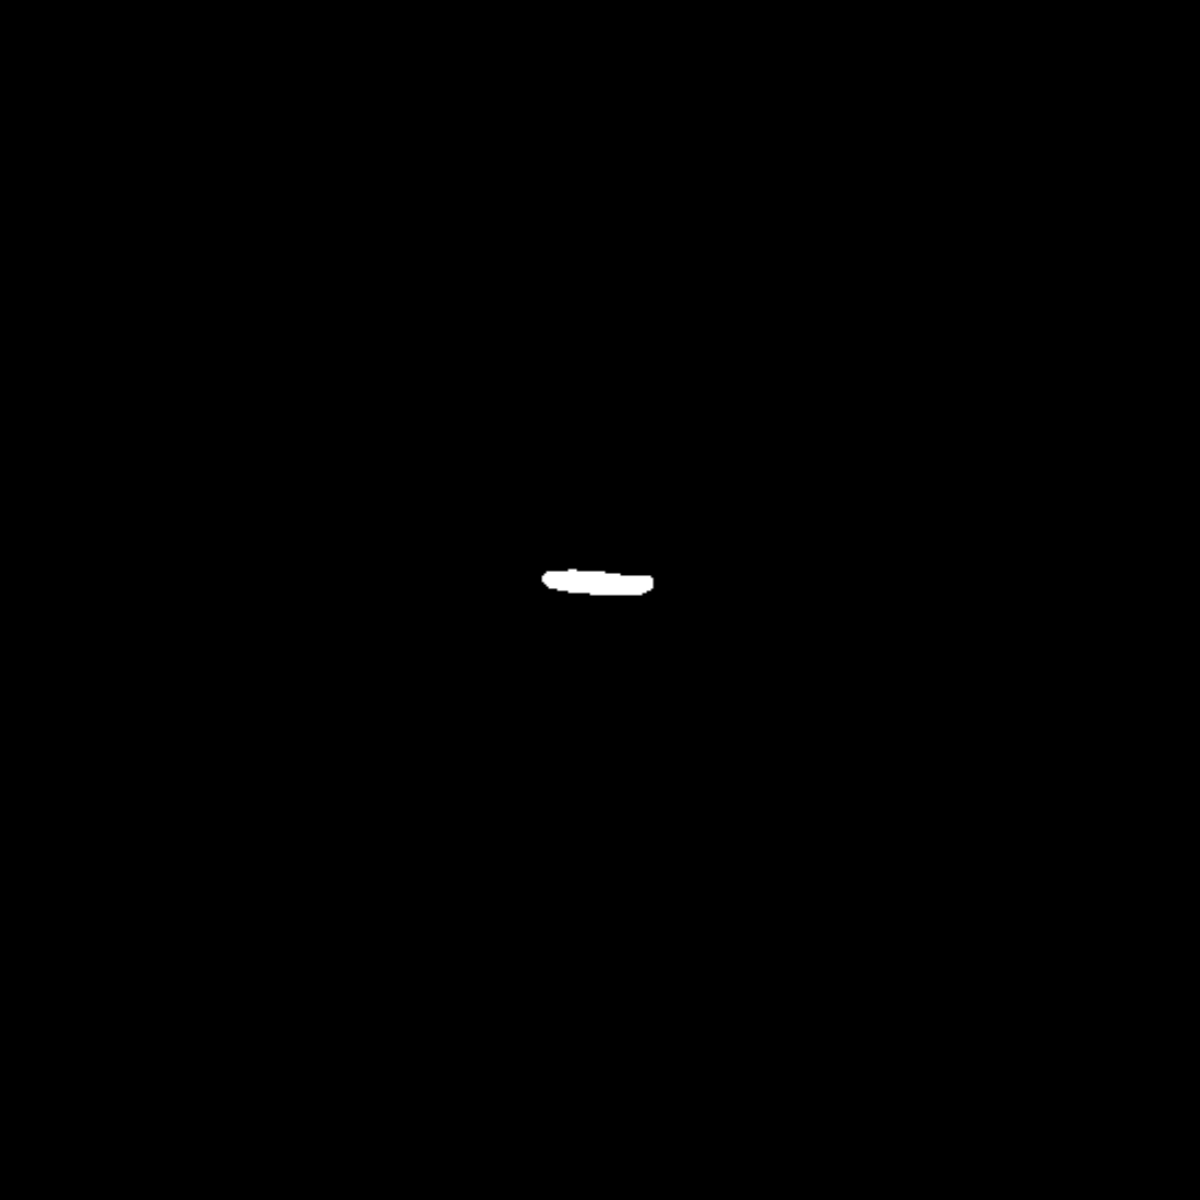
\includegraphics[width=\linewidth]{images/cluster_after.PNG}
        \caption{Final mask after background subtraction}
    \end{subfigure}
    \caption{Example showing the complementarity between color clustering and depth-based background subtraction. The clustering stage initially includes an additional region outside the dough, which is then removed by enforcing consistency with the reference table model.}
    \label{fig:cluster_bgs_example}
\end{figure}
\subsubsection{3D Completion and Volume Estimation}
After foreground extraction, the visible dough points provide only a 2.5D observation of the object. To estimate the hidden lower portion, the implementation supports several completion strategies, including axis-construction modes based on PCA and variants explicitly tied to the support surface.\cite{labby_thesis_repo_2026} In the workflow adopted for the main experiments, the rotated estimators use the \texttt{mid\_support\_pca} strategy: the direction of the rotation axis is derived from PCA on the visible and already filtered dough cloud, while the axis itself is translated so as to lie halfway between the foreground and the support plane. This placement provides a more plausible geometric center for the subsequent rotational completion.

\begin{figure}[H]
    \centering
    \begin{subfigure}[b]{0.48\textwidth}
        \centering
        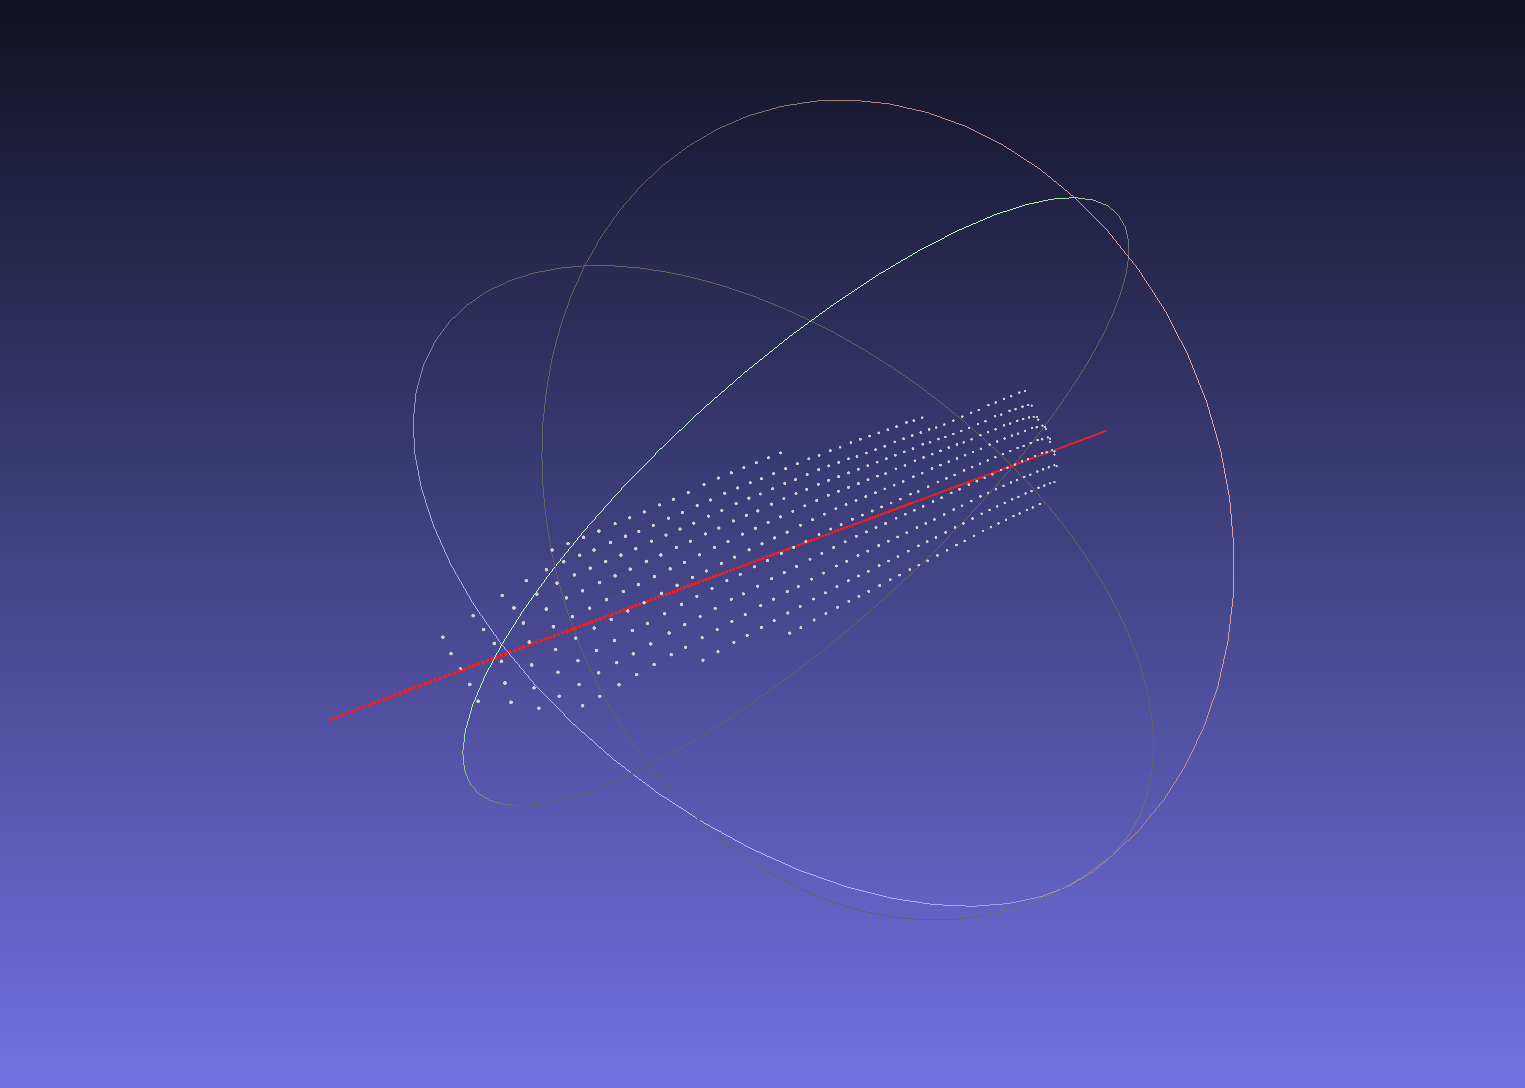
\includegraphics[width=\linewidth]{images/PCA.png}
        \caption{Visible point cloud with rotation axis}
    \end{subfigure}
    \hfill
    \begin{subfigure}[b]{0.48\textwidth}
        \centering
        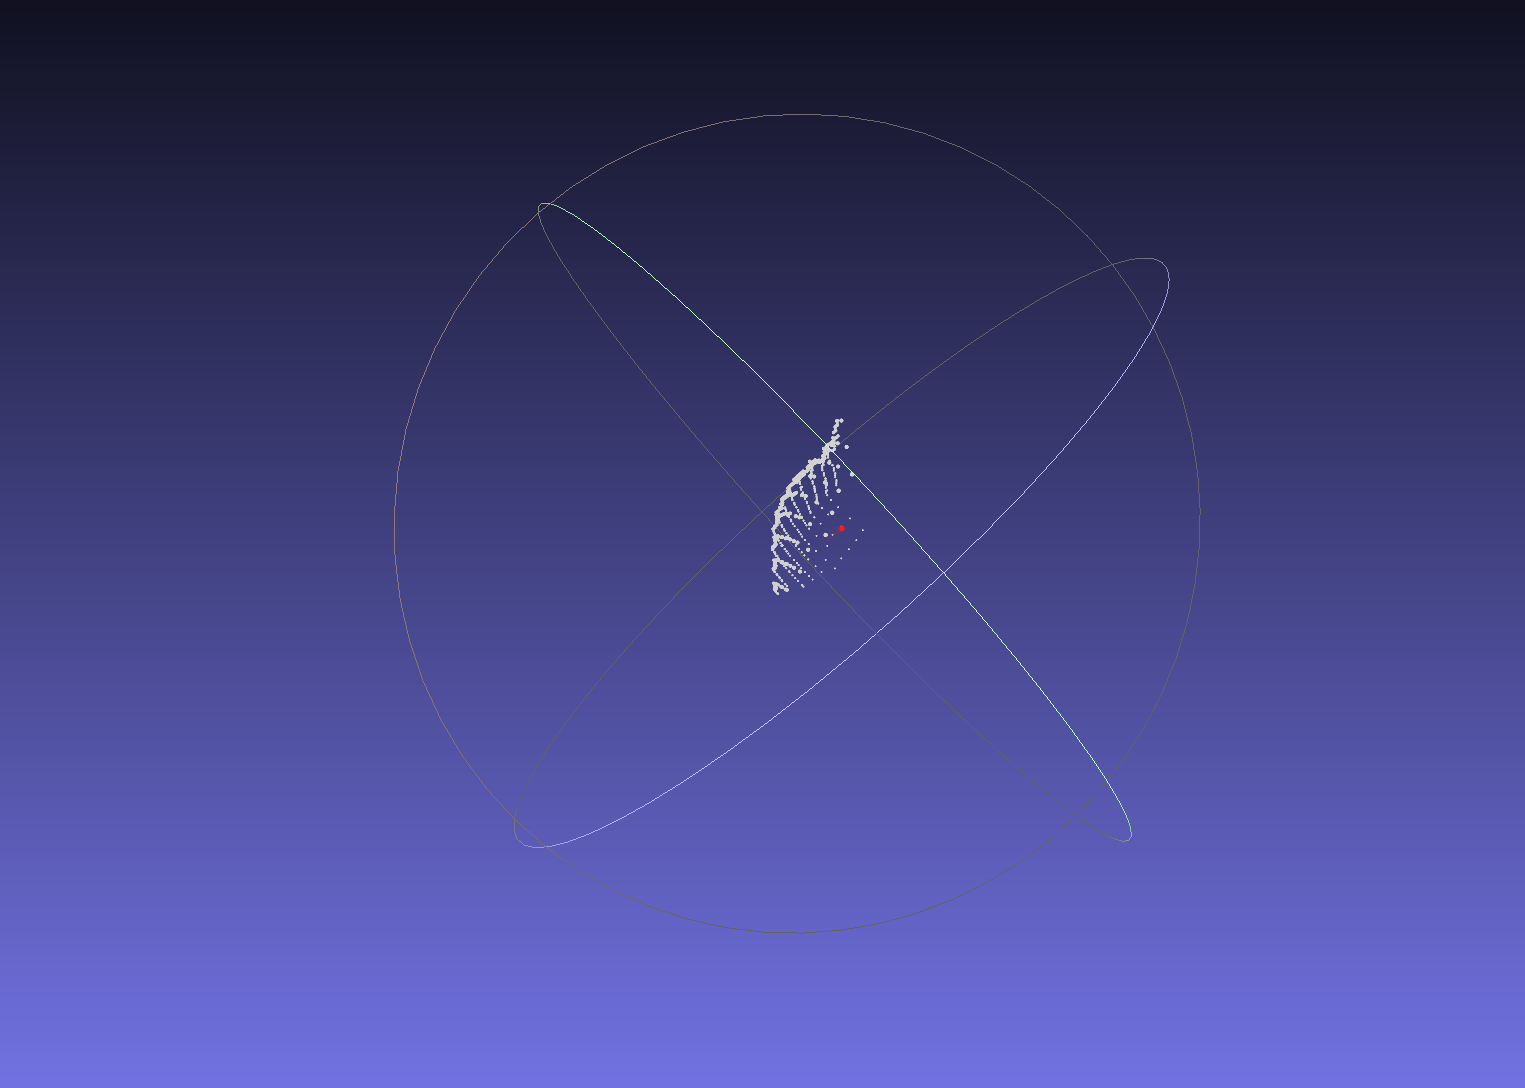
\includegraphics[width=\linewidth]{images/PCA_side.png}
        \caption{Side view of the same configuration}
    \end{subfigure}

    \vspace{0.5em}

    \begin{subfigure}[b]{0.60\textwidth}
        \centering
        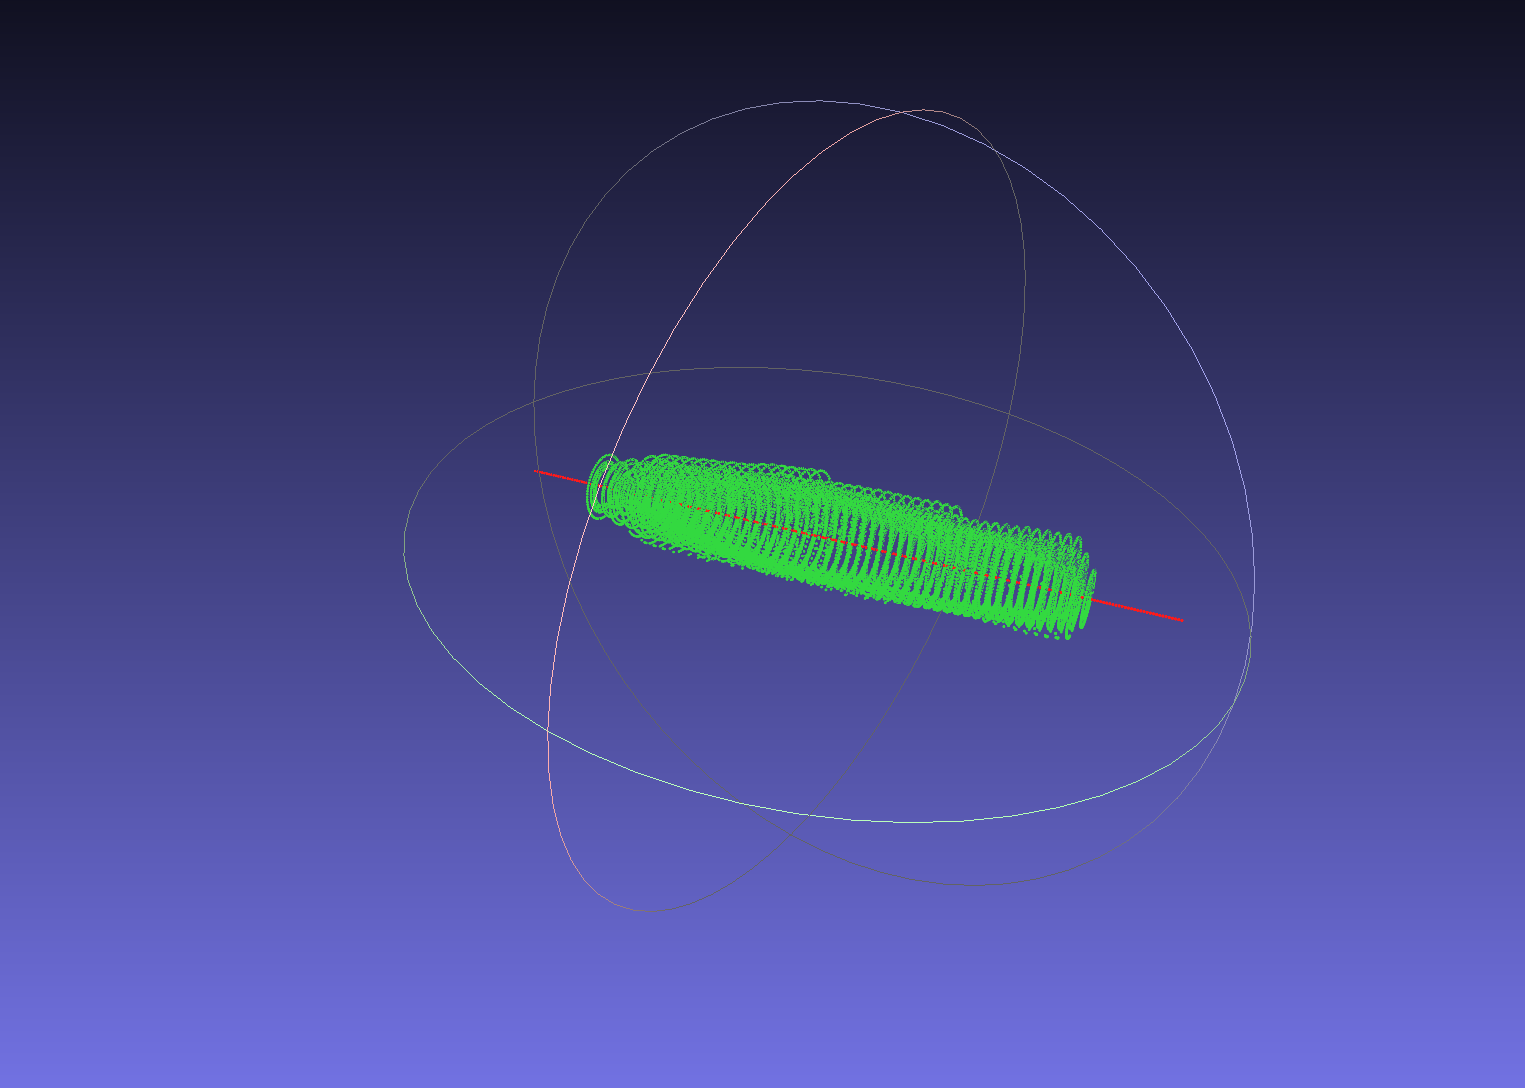
\includegraphics[width=\linewidth]{images/rotated_pc.png}
        \caption{Point cloud after rotational completion}
    \end{subfigure}
    \caption{Example of the geometric completion stage. The first two views show the visible dough point cloud together with the adopted rotation axis (in red), while the third view shows the completed point cloud obtained after rotation.}
    \label{fig:rotation_completion_example}
\end{figure}

The observed geometry is then rotated around this axis, using Rodrigues-based rigid rotations, in order to synthesize an approximation of the non-visible part of the dough. This rotational completion is used only for the rotated convex-hull and rotated alpha-shape estimators. After rotation, points that are geometrically inconsistent with the support model are discarded, and an additional statistical outlier removal stage is applied so that isolated or unstable points do not disproportionately affect the final volume estimate. This cleaning stage is especially important for the rotated estimators, since residual singular depth points near the border of the support can otherwise have a disproportionately large impact when the completion rotates them, leading to a much larger volume estimate.
\\The completed point cloud is then passed to different geometric volume estimators. A raw convex hull computed directly from the visible cloud is used only as an initial baseline and is not retained for the final comparative analysis.

\textbf{Rotated convex hull.} A convex hull is computed after rotational completion of the dough geometry.
\begin{figure}[!htbp]
    \centering
    \begin{subfigure}[b]{0.54\textwidth}
        \centering
        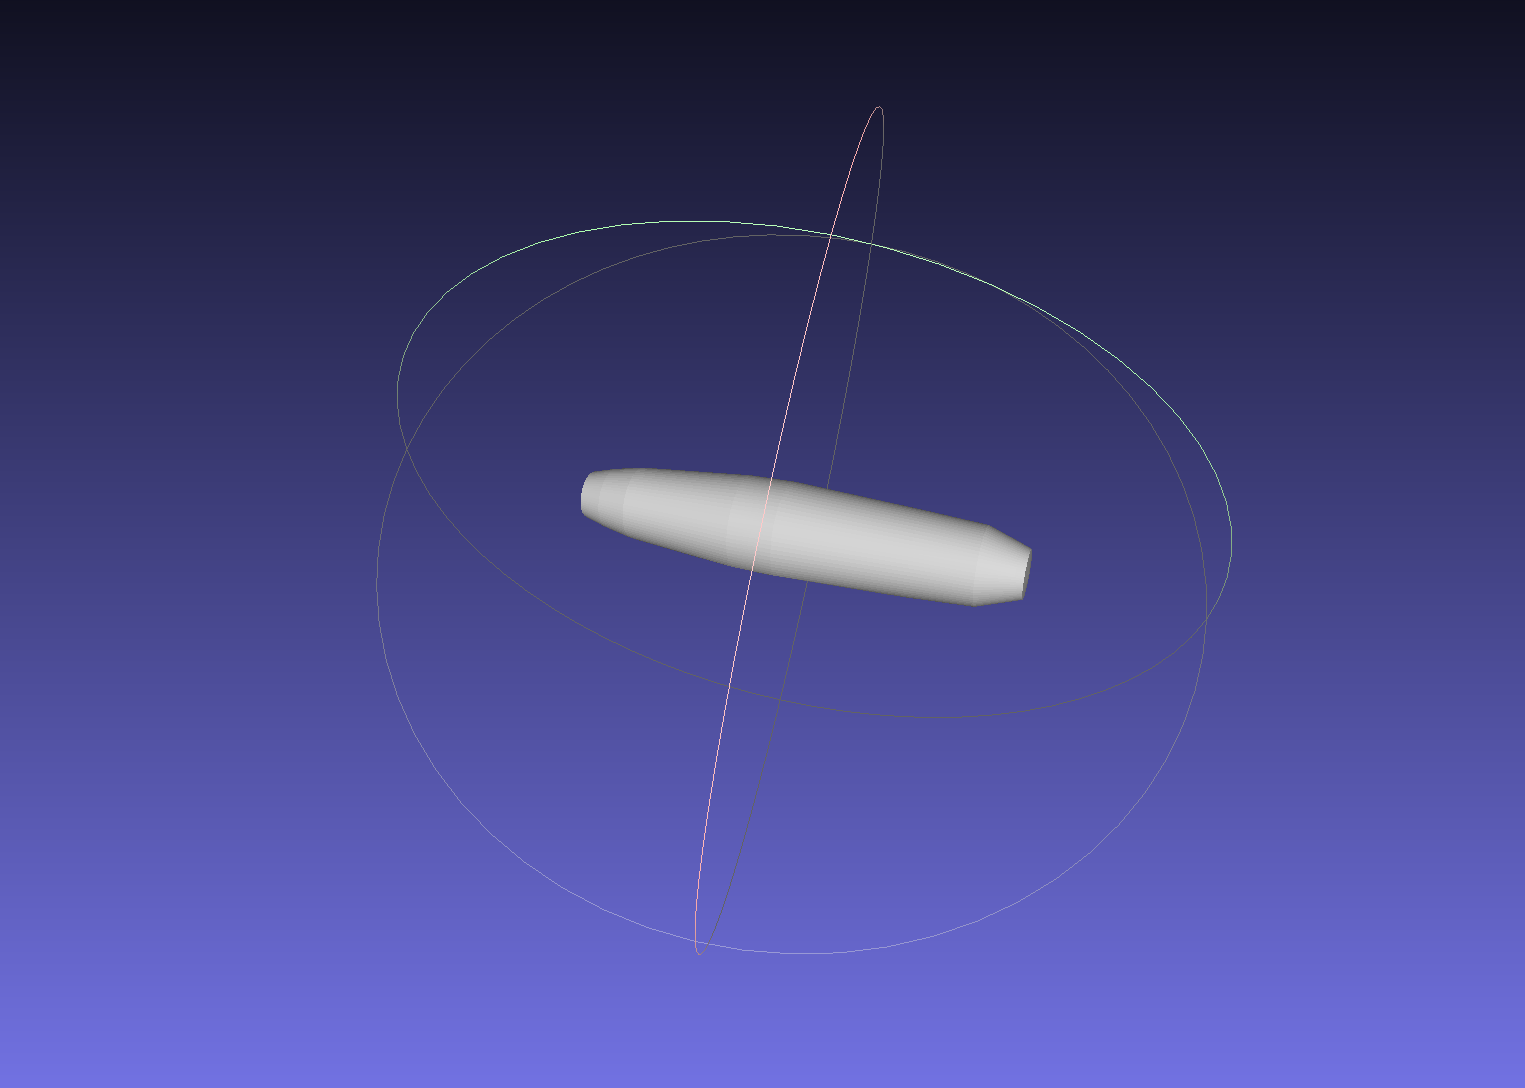
\includegraphics[width=\linewidth]{images/convex.png}
        \caption{Convex-hull mesh}
    \end{subfigure}

    \vspace{0.5em}

    \begin{subfigure}[b]{0.48\textwidth}
        \centering
        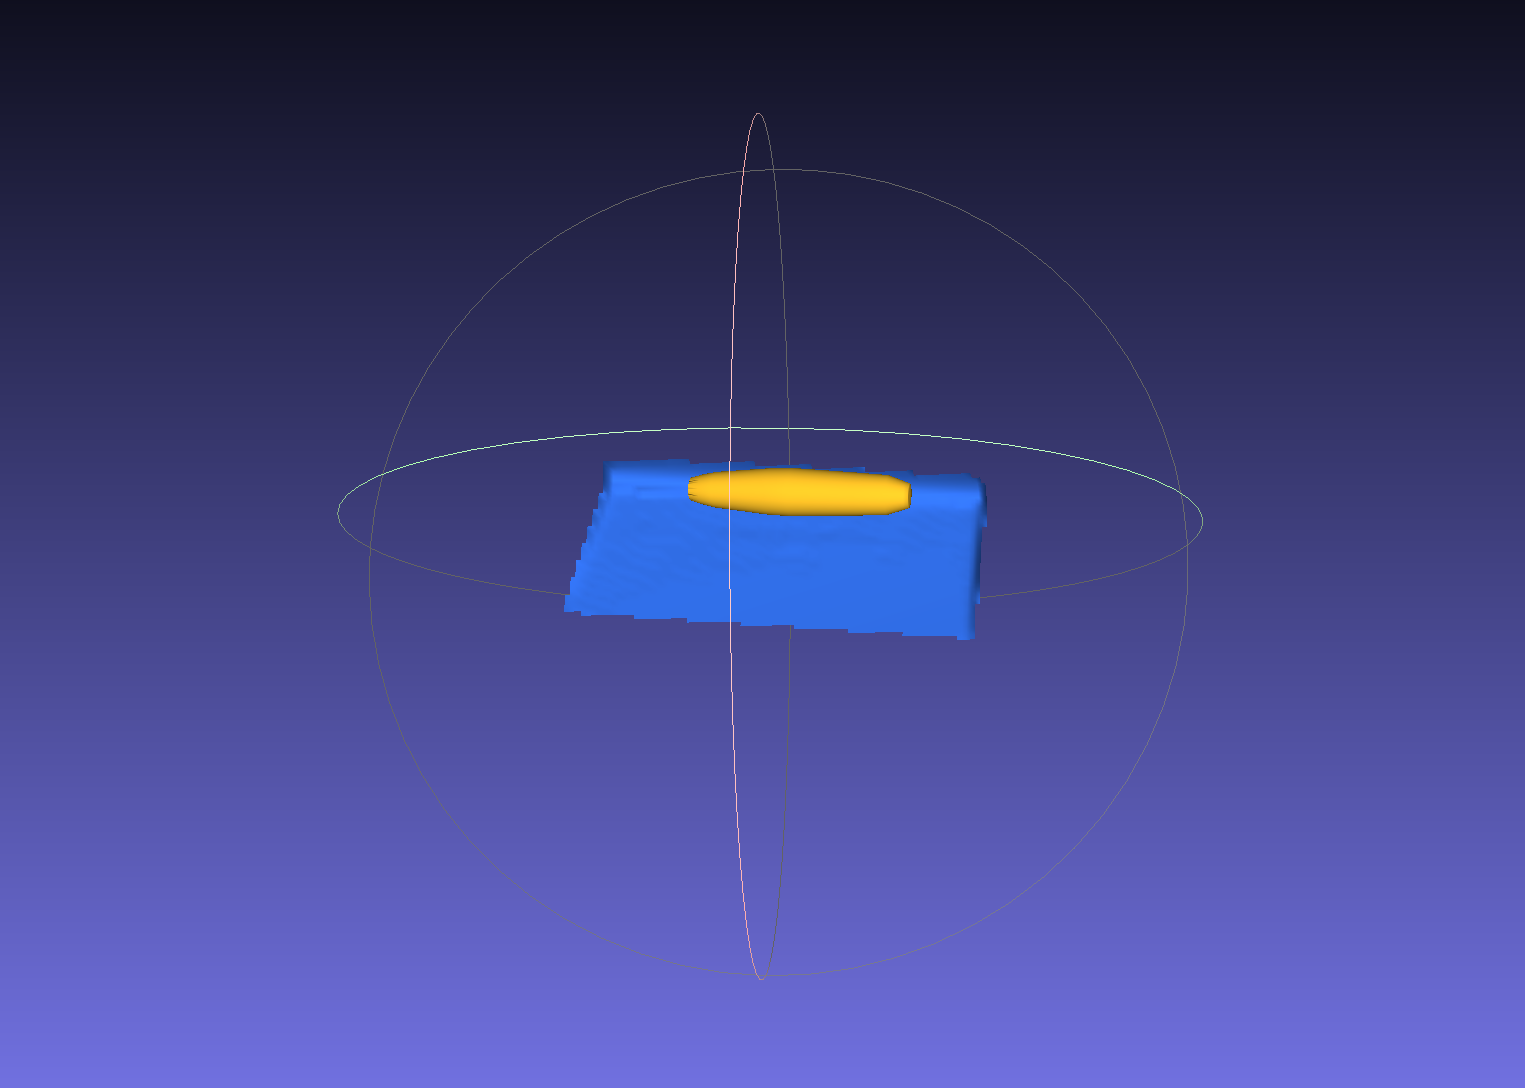
\includegraphics[width=\linewidth]{images/convex_hull_table.png}
        \caption{Front view on the reference table}
    \end{subfigure}
    \hfill
    \begin{subfigure}[b]{0.48\textwidth}
        \centering
        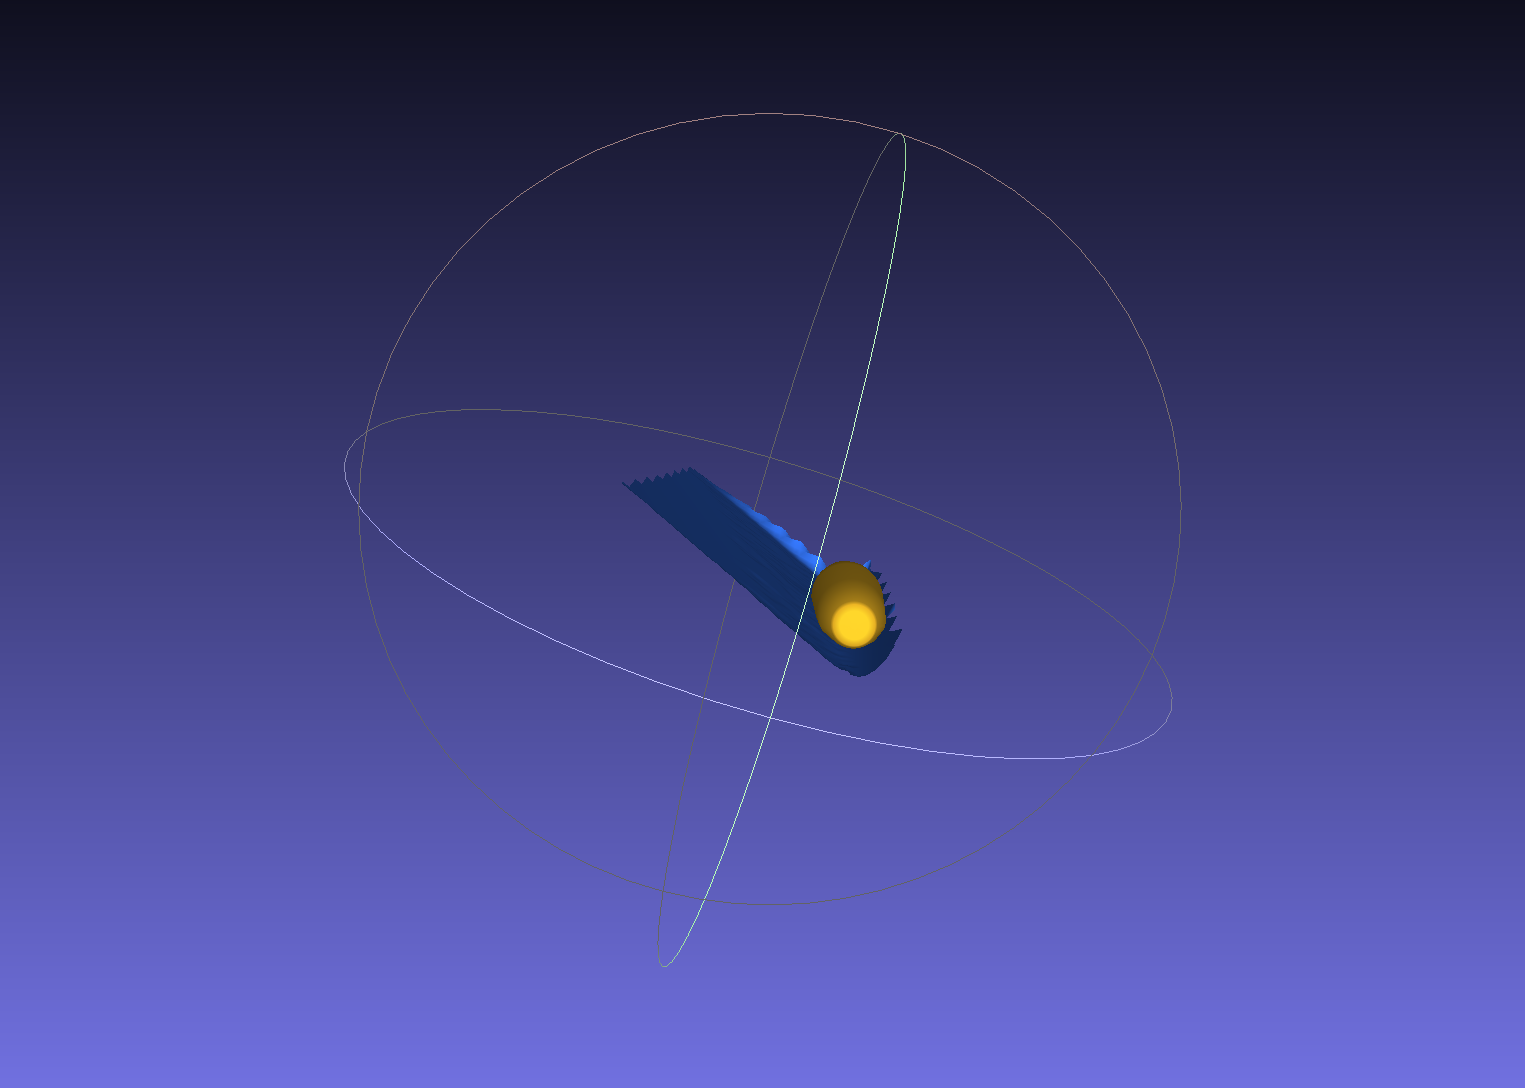
\includegraphics[width=\linewidth]{images/convex_hull_table_side.png}
        \caption{Side view on the reference table}
    \end{subfigure}
    \caption{Representative output of the rotated convex-hull estimator.}
    \label{fig:convex_hull_estimator}
\end{figure}
\newpage
\textbf{Rotated alpha shape.} An alpha-shape reconstruction is computed after rotational completion of the dough geometry.

\begin{figure}[!htbp]
    \centering
    \begin{subfigure}[b]{0.54\textwidth}
        \centering
        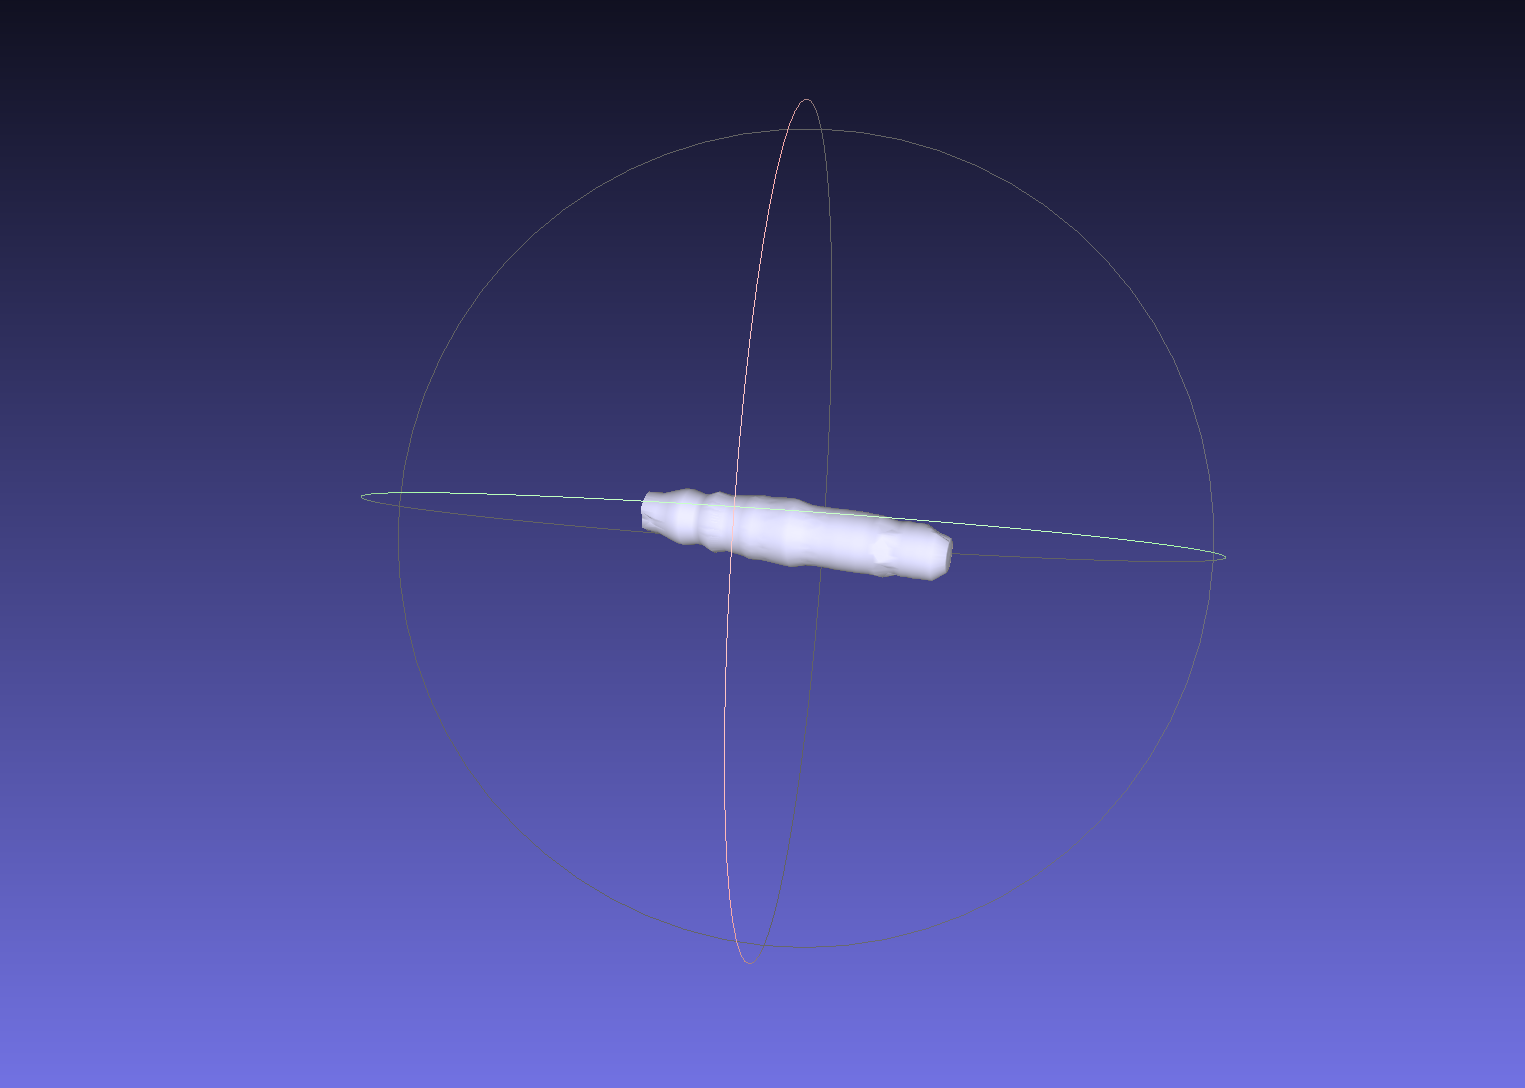
\includegraphics[width=\linewidth]{images/alpha.png}
        \caption{Alpha-shape mesh}
    \end{subfigure}

    \vspace{0.5em}

    \begin{subfigure}[b]{0.48\textwidth}
        \centering
        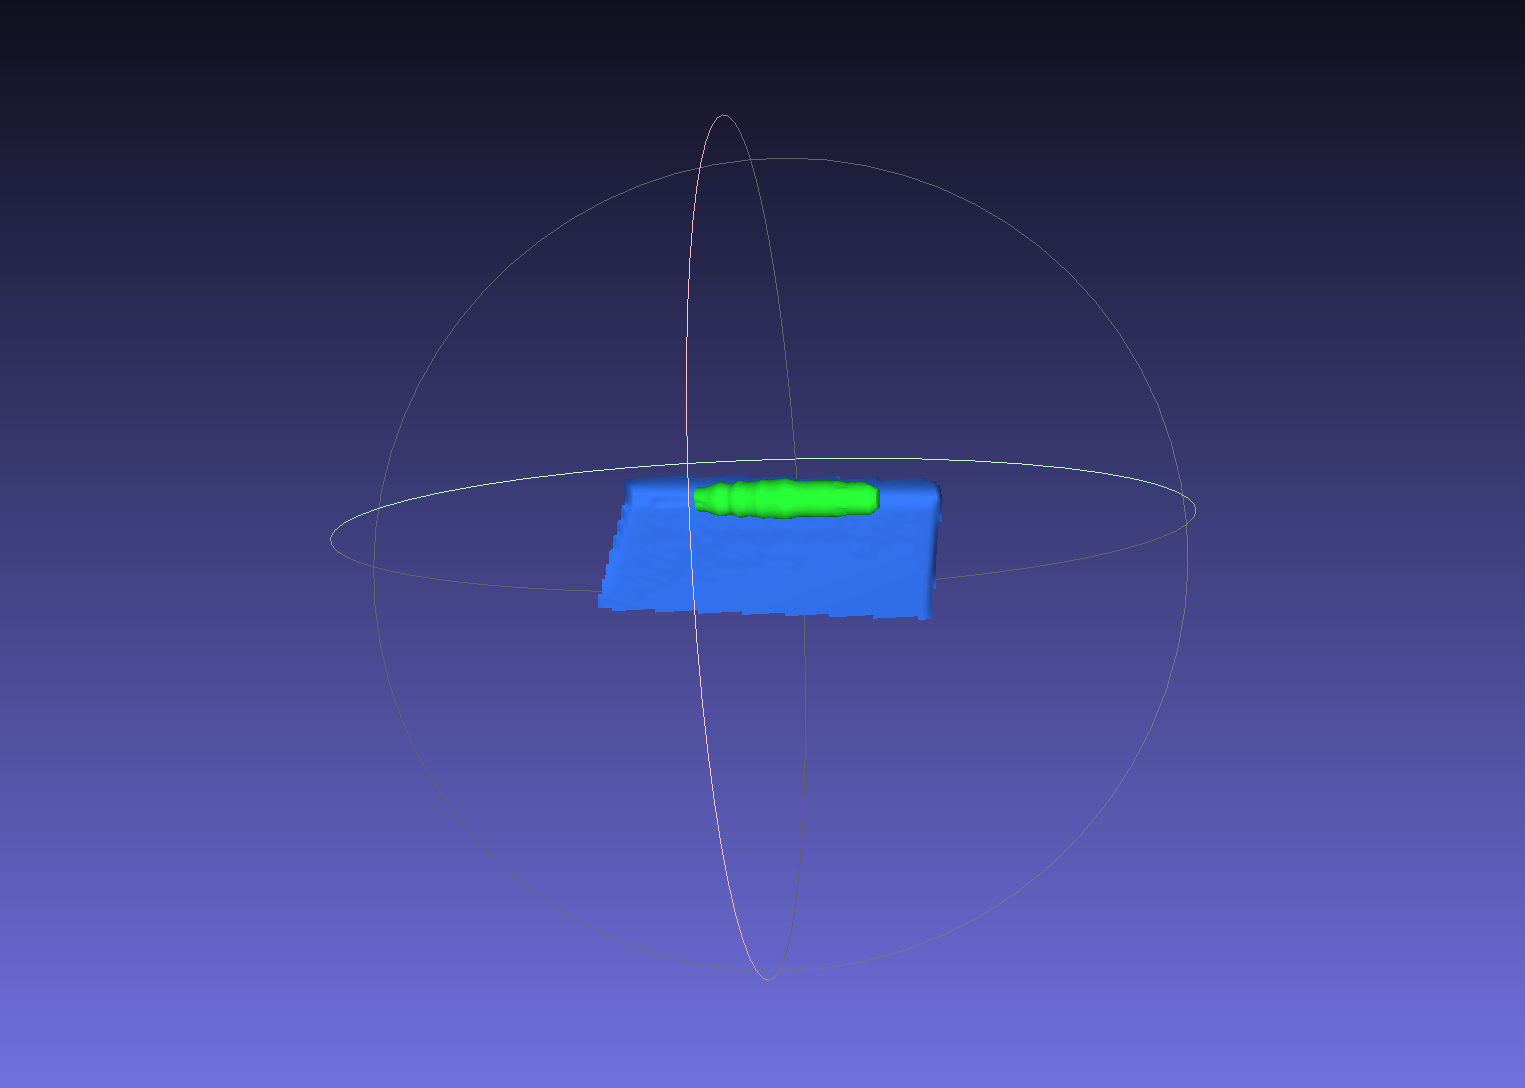
\includegraphics[width=\linewidth]{images/alpha_shape_table.png}
        \caption{Front view on the reference table}
    \end{subfigure}
    \hfill
    \begin{subfigure}[b]{0.48\textwidth}
        \centering
        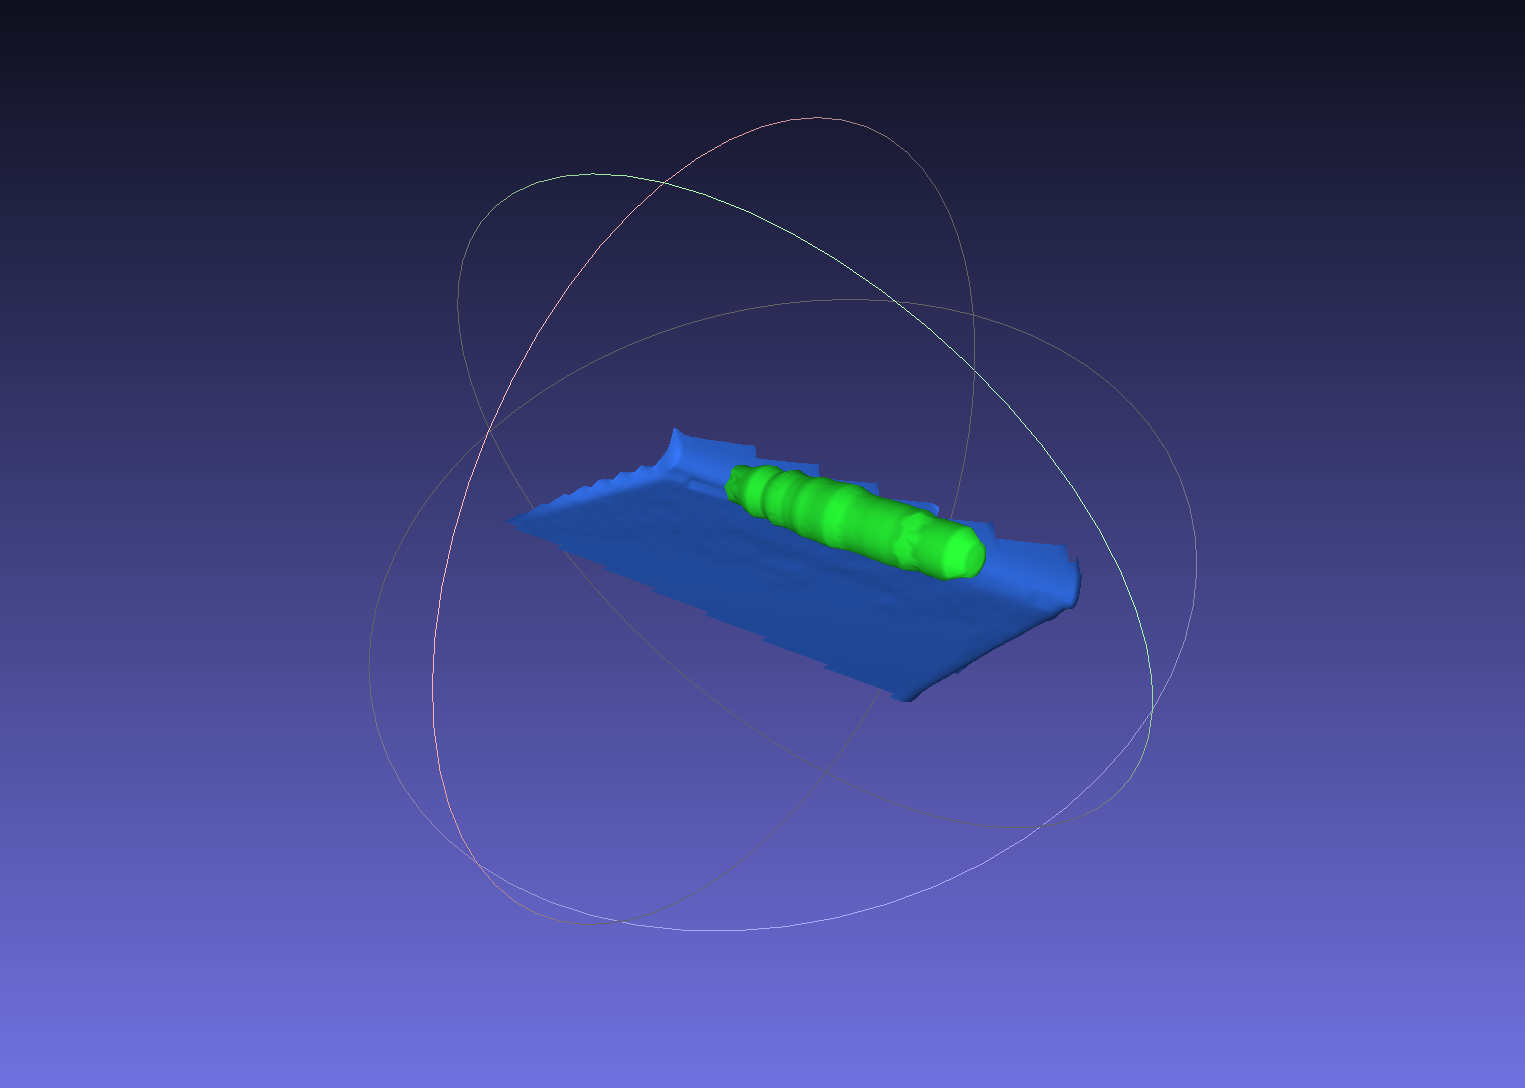
\includegraphics[width=\linewidth]{images/alpha_shape_table_side.png}
        \caption{Side view on the reference table}
    \end{subfigure}
    \caption{Representative output of the rotated alpha-shape estimator.}
    \label{fig:alpha_shape_estimator}
\end{figure}
\newpage
\textbf{Depth-gap estimator.} The \emph{depth-gap} method follows a different logic and does not rely on rotational completion. Instead, it directly fills the space between the segmented foreground and the reference support model.

\begin{figure}[H]
    \centering
    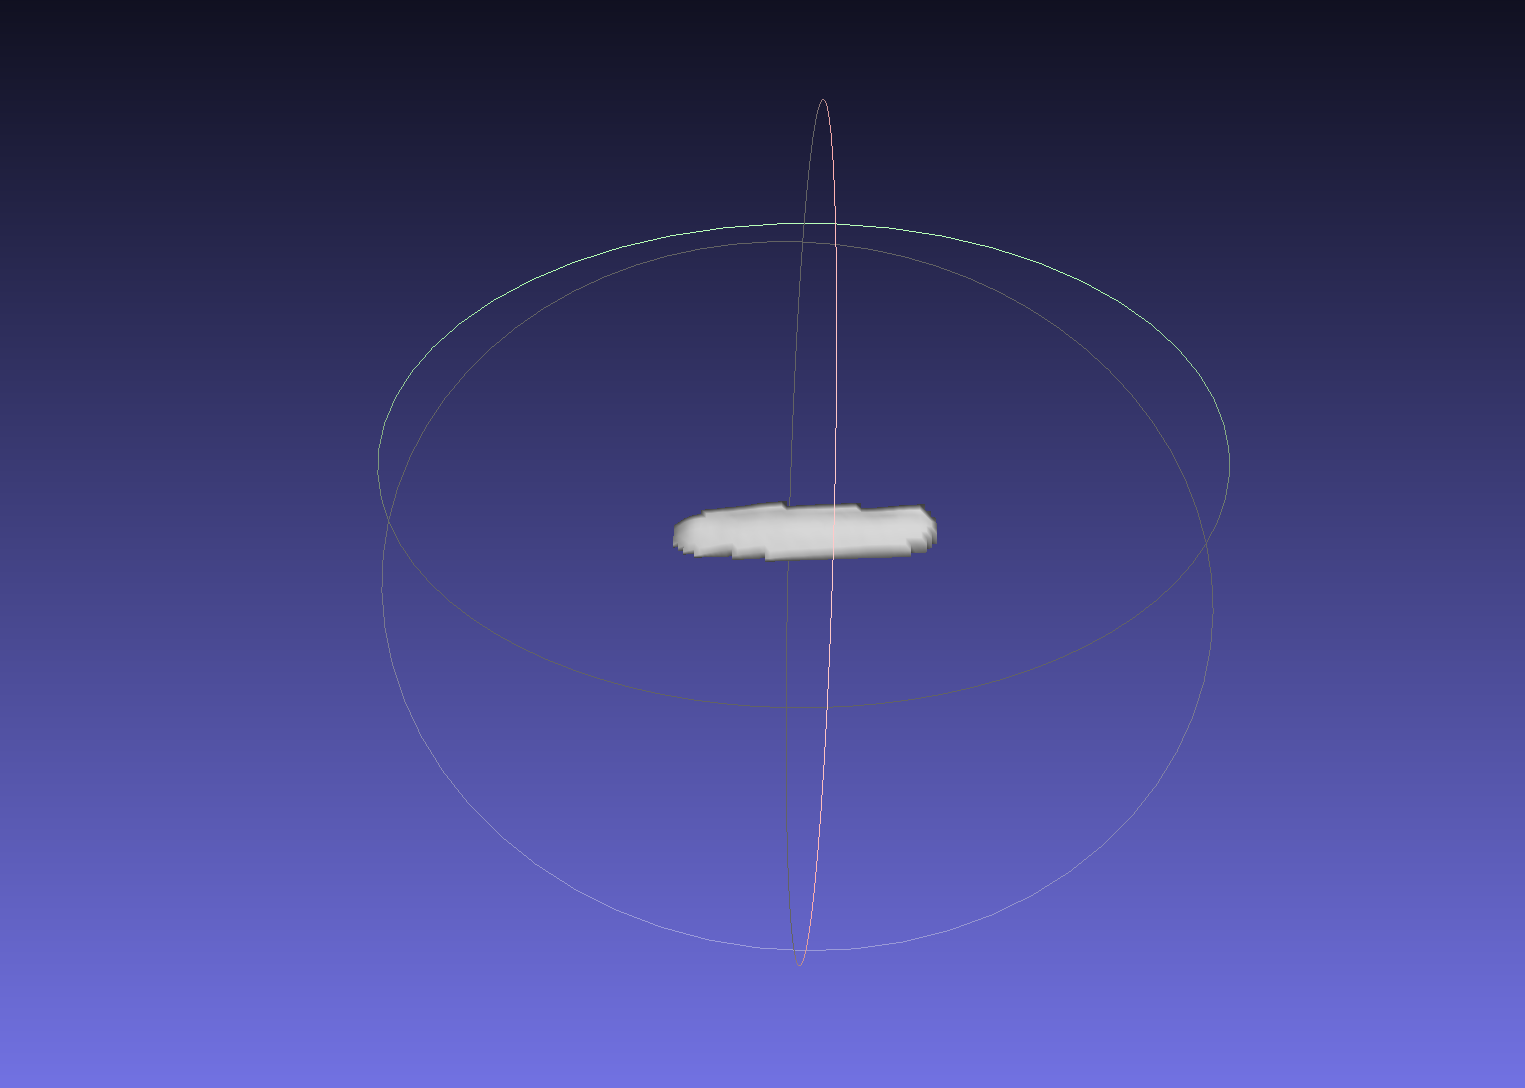
\includegraphics[width=0.70\textwidth]{images/gap.png}
    \caption{Representative output of the \emph{depth-gap} estimator.}
    \label{fig:depth_gap_estimator}
\end{figure}

Representative outputs of the three main estimators considered in this thesis are shown in Figures~\ref{fig:convex_hull_estimator}, \ref{fig:alpha_shape_estimator}, and \ref{fig:depth_gap_estimator}. The full implementation therefore makes it possible to compare simple geometric baselines with progressively more structured reconstructions. In the comparative analysis reported in this thesis, the three main estimators considered over the entire test set are the rotated convex hull, the rotated alpha shape, and the depth-gap method. Their resulting volume distributions are then analyzed and compared in order to assess the consistency of the reconstructed dough volumes, as discussed in Chapter~5.
\newpage
\subsection{Site 2: Anomaly Detection}
At Site~2, the downstream task is not geometric reconstruction but visual anomaly assessment of the final baked product. For this reason, the anomaly-detection branch operates on localized loaf crops rather than on full production-line frames. In the implemented framework, these crops are processed by EfficientAD through anomalib, so that each loaf can be assigned an image-level anomaly score together with spatial diagnostic outputs such as anomaly maps and predicted masks.\cite{batzner_efficientad_2024,akcay_anomalib_2022}

\subsubsection{Dataset Preparation from Loaf Crops}
The first step of the anomaly-detection branch consists of exporting bread-loaf crops from the detector annotations. A dedicated utility reads COCO-style bounding-box annotations, optionally enlarges the crop through configurable padding, discards excessively small detections, and organizes the resulting images into a structure compatible with anomaly-detection training.\cite{labby_thesis_repo_2026}

Two complementary dataset-construction strategies are supported. The first is a simple automatic split, which partitions the crops into train, validation, and test sets according to a 0.8/0.1/0.1 ratio. The second is an interactive review tool through which exported crops can be inspected and manually assigned to good or defective/anomalous subsets before being distributed across the dataset folders.\cite{labby_thesis_repo_2026} This strategy is particularly useful when anomalous samples are few, heterogeneous, externally sourced, or when a small but carefully controlled exploratory dataset is needed. In the present work, this tool was also used in a preliminary test on about 300 good samples, while crops partially occluded by a hand or by the tray were operationally assigned to the defect group. The aim of this test was not to define a representative taxonomy of industrial defects, but to verify whether the network could rapidly separate clearly non-good samples from the good dataset in the event that defective products became available during operation. Since the results of this preliminary test were promising, the model was then trained on the full collected dataset, which was subsequently partitioned into training, validation, and test subsets according to the adopted split.

In the experiments described in this thesis, the normal class is composed of \emph{good} bread images collected during the two-week acquisition campaign. Since no representative defective loaves were provided either by the production site or by the SMACT \cite{smact_official_2026} operators, \textbf{the collected on-site dataset was treated as entirely normal}. To obtain an initial qualitative indication of the model behavior on clearly non-conforming products, a small auxiliary set of \textbf{18 defective bread images} collected \textbf{from online sources} was used as an external reference, with 9 images assigned to the validation set and 9 distinct images assigned to the test set. These images were not used to define the normal training distribution, but only as auxiliary anomalous examples for preliminary qualitative evaluation. They depict clearly non-conforming products, such as burnt or mouldy loaves, but they are not fully representative of either the bread type or the visual environment observed in the industrial setup.

\begin{figure}[H]
    \centering
    \begin{subfigure}[b]{0.24\textwidth}
        \centering
        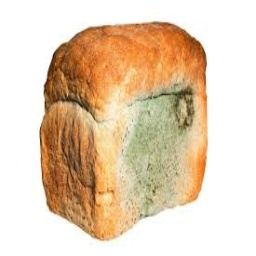
\includegraphics[width=\linewidth]{images/defect1 (1).jpg}
    \end{subfigure}
    \hfill
    \begin{subfigure}[b]{0.24\textwidth}
        \centering
        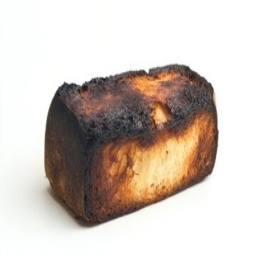
\includegraphics[width=\linewidth]{images/defect1 (2).jpg}
    \end{subfigure}
    \hfill
    \begin{subfigure}[b]{0.24\textwidth}
        \centering
        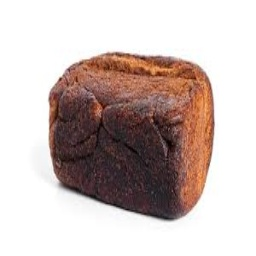
\includegraphics[width=\linewidth]{images/defect1 (3).jpg}
    \end{subfigure}
    \hfill
    \begin{subfigure}[b]{0.24\textwidth}
        \centering
        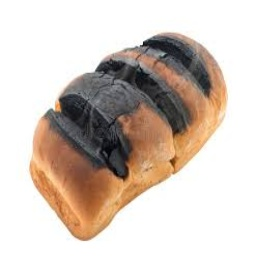
\includegraphics[width=\linewidth]{images/defect1 (4).jpg}
    \end{subfigure}
    \caption{Examples of externally sourced defective bread images used only for qualitative validation and testing of the anomaly-detection branch.}
    \label{fig:site2_external_defects}
\end{figure}

For this reason, they are not expected to provide a rigorous estimate of industrial anomaly-detection performance; rather, they offer a \textbf{practical sanity check} for the anomaly scores and maps produced by the trained model.\cite{labby_thesis_repo_2026} This choice remains consistent with the one-class training paradigm, which focuses on learning the normal class and then relies on anomaly scores to identify deviations from that normality, even when the specific nature of the anomalies is not known in advance.\cite{batzner_efficientad_2024}

\subsubsection{EfficientAD Training}
Once the loaf crops have been organized, EfficientAD is trained through anomalib.\cite{akcay_anomalib_2022} The method remains one-class: it learns the appearance of normal bread from the training set of good samples and later measures deviations from this learned normality at inference time.\cite{batzner_efficientad_2024} Accordingly, the actual training phase is based on the normal samples only, whereas any external anomalous examples are reserved for exploratory validation or qualitative inspection.

The training scripts are designed to be practical for real experimentation. They expose parameters such as image size, batch size, mixed-precision usage, and validation limits, thereby making it possible to adapt the training run to the available GPU memory.\cite{labby_thesis_repo_2026} The implementation also supports scenarios in which anomalous validation or test samples are absent, while still allowing external anomalous images to be included in the validation or test folders whenever a preliminary qualitative check is needed. In this way, the same codebase can be used both for strict one-class training and for exploratory validation of anomaly scores on externally sourced defect examples.

\subsubsection{Inference and Reporting}
After training, the best checkpoint is loaded for inference on batches of loaf crops. Because large inference sets may exceed memory or I/O limits if processed at once, the repository includes a chunked inference routine that iterates over the dataset in manageable groups and stores the predictions incrementally.\cite{labby_thesis_repo_2026}

For each analyzed crop, the implemented pipeline produces an image-level anomaly score, a predicted class label, an anomaly map, and a binary mask. The outputs are then saved both in numerical form, through CSV and text summaries, and in visual form, through heatmaps, overlays, and dedicated debug folders containing the most anomalous examples.\cite{labby_thesis_repo_2026} In the context of this thesis, the most relevant quantity is the anomaly score itself, since it provides the scalar measure used to compare samples and to analyze the distribution of potentially problematic loaves over the inspected set.
These results are then shown and analyzed in Chapter~5.

 %File in cui è scritto il capitolo
\label{chapter:chapter_5} %Label per creare riferimenti al capitolo
% !TeX root = ../../tesi.tex

\chapter{Results}
\section{Site 1: dough-ball volume estimation}
\subsection{Quantitative results}
\subsection{Qualitative results}
\section{Site 2: bread quality assessment}
\subsection{Quantitative results}
\subsection{Anomaly score heatmaps}
 %File in cui è scritto il capitolo
\label{chapter:chapter_6} %Label per creare riferimenti al capitolo
\chapter{Conclusion and future works}
In this thesis, we presented a multimodal quality inspection framework for the food industry, specifically designed for the bread production process. The framework integrates various techniques, including motion detection, DEIMv2 training, and feature extraction, to assess the quality of dough balls and bread products. The implementation of the framework was carried out using OpenCV, Open3D, Torch, and Tensorboard, demonstrating the practical application of these tools in an industrial setting.
The results obtained from the framework showed promising outcomes in terms of dough-ball volume estimation and bread quality assessment. The quantitative and qualitative results for both Site 1 and Site 2 indicated that the framework is effective in monitoring the production process and identifying potential quality issues.
Future works could focus on further improving the accuracy and efficiency of the framework, as well as exploring additional features and techniques for quality inspection. This could include the integration of more advanced machine learning models, the use of additional sensors for data collection, and the development of real-time monitoring capabilities to provide immediate feedback during the production process. Additionally, expanding the framework to other food products and industries could further demonstrate its versatility and applicability in various manufacturing contexts. %File in cui è scritto il capitolo



%%%%%%%%%%%%%%%% BIBLIOGRAFIA
\clearpage{\pagestyle{plain}\cleardoublepage}
{\small
\bibliographystyle{model/biblio_style}
\bibliography{start-end/reference}
}

\end{document}
